% ******************************* PhD Thesis Template **************************
% Please have a look at the README.md file for info on how to use the template

\documentclass[a4paper,12pt,times,authoryear,print,twoside,index]{PhDThesisPSnPDF}



\usepackage[utf8]{inputenc} %The package translates various standard and other input encoding into a ‘LATEX internal language’. Acentos graficos e etc...
\usepackage[T1]{fontenc} %The T1 font encoding is an 8-bit encoding and uses fonts that have 256 glyphs.
\usepackage{mathptmx} % Font Times New Rome
\usepackage[english]{babel} % English language/hyphenation
\usepackage{graphicx} %The graphicx package provides the includegraphics command.
\usepackage{amssymb} %The amssymb package provides various useful mathematical symbols
\usepackage{amsthm} %% The amsthm package provides extended theorem environments
\usepackage{natbib} %bibliography
\bibliographystyle{abbrvnat}
\setcitestyle{authoryear,open={(},close={)}}
%\setlength\bibindent{0pt}
\usepackage{marvosym} %font style
\usepackage{amsfonts} %An extended set of fonts for use in mathematics, including: extra mathematical symbols
%\usepackage{fourier} %font package with extra mathematical symbols
\usepackage{amsmath,amssymb}% Math packages
\DeclareMathOperator{\E}{\mathbb{E}}
\usepackage{amsthm}
\usepackage{url} %form of verbatim command that allows line breaks at certain characters or combinations of characters, accepts reconfiguration, and can usually be used in the argument to another command.
%\usepackage[titletoc,title]{appendix} %force Latex to use "Appendix A" without giving a name in place of the simple "A".
\usepackage{graphicx,subfigure} %Add 2 figures in a row
%\usepackage{subfig} % The package provides support for the manipulation and reference of small or ‘sub’ figures and tables within a single figure or table environment.
\usepackage[labelfont=bf]{caption} % Facilities include rotating captions, sideways captions, continued captions (for tables or figures that come in several parts).  %Bold Font for Captions Fig 2.1
\captionsetup{justification=raggedright,singlelinecheck=false} %Allows the caption to be lefthand-side
%\usepackage{subcaption} %Same as subfigure
\usepackage{afterpage} % Provides a means of running commands immediately after the current page is output
\usepackage{epigraph} %EpigrGTphs are the pithy quotations often found at the start (or end) of a chapter.
\usepackage[bottom]{footmisc} %Place the footnote at the bottom of the page.
\pretolerance=100000 %an integer parameter that is used in TeX's line breaking algorithm.
\usepackage{float} %is about the floating environments figure, table and other, custom-defined floats, and concerns issues such as positioning, labelling, captioning, indexing and listing of said floats.
%\widowpenalties 1 100 %Penalty for a broken page, with a single line of a paragraph (called "widow") remaining on the top of the succeeding page.
\usepackage{etoolbox} %Macro for Author packages
\usepackage{stfloats} % provide commands to control \baselineskip, that actually permit stretch and shrink, allowing a different value for use within floats; provide commands to control whether footnotes will appear above (as standard) or below a bottom float;provides a command that declares that double floats should be placed at the bottom (rather than the top) of a page.
\usepackage{rotating} %A package built on the standard LATEX graphics package to perform all the different sorts of rotation one might like, including complete figures and tables with their captions.
\usepackage{booktabs} %The package enhances the quality of tables in LATEX, providing extra commands as well as behind-the-scenes optimisation.
\usepackage[doublespacing]{setspace} %setting the space between the lines
\usepackage{upquote} %The package switches the typewriter font to Computer Modern Typewriter in OT1 encoding, and modifies the behaviour of verbatim, verbatim*, \verb, and \verb* to print in the “` and ' way”. It does this regardless of other fonts or encodings in use, so long as the package is loaded after the other fonts were.
\usepackage{listings} %The package enables the user to typeset programs (programming code) within LATEX.
\usepackage{enumerate} %The package adds an optional argument to the enumerate environment which determines the style in which the counter is printed.
\usepackage{lscape} %Modifies the margins and rotates the page contents but not the page number. Useful, for example, with large multipage tables, as it is compatible with longtable and supertabular.
\usepackage{verbatim} % package to include commenting out sections
\usepackage{pdflscape} %The package adds PDF support to the landscape environment of package lscape, by setting the PDF /Rotate page attribute. Pages with this attribute will be displayed in landscape orientation by conforming PDF viewers.
\usepackage{bm} %package defines a command \bm which makes its argument bold. The argument may be any maths object from a single symbol to an expression
\usepackage[pdftex]{hyperref} %The hyperref package is used to handle cross-referencing commands in LATEX to produce hypertext links in the pdf document.
\hypersetup{
    colorlinks=false,
    linkcolor=black,
    filecolor=black,      
    urlcolor=black,
}
\usepackage{pdfpages} %This package simplifies the inclusion of external multi-page PDF documents in LATEX documents. Pages may be freely selected and similar to psnup it is possible to put several logical pages onto each sheet of paper.
\usepackage{dcolumn} %The dcolumn package makes use of the array package to define a "D" column format for use in tabular environments.
\usepackage{longtable} %Longtable allows you to write tables that continue to the next page.
\usepackage[export]{adjustbox} %The package provides several macros to adjust boxed content. One purpose is to supplement the standard graphics package, which defines the macros \resizebox, \scalebox and \rotatebox , with the macros\trimbox and \clipbox.
%\usepackage{menukeys}
\usepackage{booktabs}
\usepackage{tabularx} %The package defines an environment tabularx, an extension of tabular which has an additional column designator, X, which creates a paragraph-like column whose width automatically expands so that the declared width of the environment is filled. (Two X columns together share out the available space between them, and so on.) Creates a table with the same width of the text.
\newcolumntype{b}{X} %Setting the width of the Table in \Tabluarx
\newcolumntype{s}{>{\hsize=.33\hsize}X} %Setting the width
\newcolumntype{T}{>{\hsize=.80\hsize}X}
\newcolumntype{A}{>{\hsize=.68\hsize}X}
\newcolumntype{B}{>{\hsize=.30\hsize}X}
\newcolumntype{Y}{>{\centering\arraybackslash}X} %centering the table
\newcolumntype{Z}{>{\centering\arraybackslash}s}
\newcolumntype{K}{>{\centering\arraybackslash}A}
\newcolumntype{C}{>{\centering\arraybackslash}B}
\usepackage{lipsum}% This package gives you easy access to the Lorem Ipsum dummy text
%\usepackage[toc,page]{appendix} %A set of macros created for use in writing the table of contents for a document
\usepackage[absolute]{textpos} %A package to facilitate placement of boxes at absolute positions on the LATEX page. There are several reasons why this might be useful, an important one being to help the creation of large-format conference posters.
%\usepackage{geometry}
% \geometry{a4paper}
\usepackage{xcolor} %Set different colours
\usepackage{tikz} %For Fluxograms
\usetikzlibrary{calc,trees,positioning,arrows,chains,shapes.geometric, decorations.pathreplacing,decorations.pathmorphing,shapes, matrix,shapes.symbols}
\usepackage{scalerel} %scales the sub-subscript
\usepackage[titletoc,toc,page,title,header]{appendix}
%\renewcommand{\appendixname}{}
%\usepackage{titlesec}

% ******************************************************************************
% ******************************* Class Options ********************************
% *********************** See README for more details **************************
% ******************************************************************************

% `a4paper'(The University of Cambridge PhD thesis guidelines recommends a page
% size a4 - default option) or `a5paper': A5 Paper size is also allowed as per
% the Cambridge University Engineering Deparment guidelines for PhD thesis
%
% `11pt' or `12pt'(default): Font Size 10pt is NOT recommended by the University
% guidelines
%
% `oneside' or `twoside'(default): Printing double side (twoside) or single
% side.
%
% `print': Use `print' for print version with appropriate margins and page
% layout. Leaving the options field blank will activate Online version.
%
% `index': For index at the end of the thesis
%
% `draftclassic': For draft mode without loading any images (same as draft in book)
%
% `draft': Special draft mode with line numbers, images, and water mark with
% timestamp and custom text. Position of the text can also be modified.
%
% `abstract': To generate only the title page and abstract page with
% dissertation title and name, to submit to the Student Registry
%
% `chapter`: This option enables only the specified chapter and it's references
%  Useful for review and corrections.
%
% ************************* Custom Page Margins ********************************
%
% `custommargin`: Use `custommargin' in options to activate custom page margins,
% which can be defined in the preamble.tex. Custom margin will override
% print/online margin setup.
%
% *********************** Choosing the Fonts in Class Options ******************
%
% `times' : Times font with math support. (The Cambridge University guidelines
% recommend using times)
%
% `fourier': Utopia Font with Fourier Math font (Font has to be installed)
%            It's a free font.
%
% `customfont': Use `customfont' option in the document class and load the
% package in the preamble.tex
%
% default or leave empty: `Latin Modern' font will be loaded.
%
% ********************** Choosing the Bibliography style ***********************
%
% `authoryear': For author-year citation eg., Krishna (2013)
%
% `numbered': (Default Option) For numbered and sorted citation e.g., [1,5,2]
%
% `custombib': Define your own bibliography style in the `preamble.tex' file.
%              `\RequirePackage[square, sort, numbers, authoryear]{natbib}'.
%              This can be also used to load biblatex instead of natbib
%              (See Preamble)
%
% **************************** Choosing the Page Style *************************
%
% `default (leave empty)': For Page Numbers in Header (Left Even, Right Odd) and
% Chapter Name in Header (Right Even) and Section Name (Left Odd). Blank Footer.
%
% `PageStyleI': Chapter Name next & Page Number on Even Side (Left Even).
% Section Name & Page Number in Header on Odd Side (Right Odd). Footer is empty.
%
% `PageStyleII': Chapter Name on Even Side (Left Even) in Header. Section Number
% and Section Name in Header on Odd Side (Right Odd). Page numbering in footer

% Uncomment to change page style
\pagestyle{PageStyleI}

% ********************************** Preamble **********************************
% Preamble: Contains packages and user-defined commands and settings
% ******************************************************************************
% ****************************** Custom Margin *********************************

% Add `custommargin' in the document class options to use this section
% Set {innerside margin / outerside margin / topmargin / bottom margin}  and
% other page dimensions
\ifsetCustomMargin
  \RequirePackage[left=40mm,right=20mm,top=35mm,bottom=30mm]{geometry}
  \setFancyHdr % To apply fancy header after geometry package is loaded
\fi

% Add spaces between paragraphs
%\setlength{\parskip}{0.5em}
% Ragged bottom avoids extra whitespaces between paragraphs
\raggedbottom
% To remove the excess top spacing for enumeration, list and description
%\usepackage{enumitem}
%\setlist[enumerate,itemize,description]{topsep=0em}

% *****************************************************************************
% ******************* Fonts (like different typewriter fonts etc.)*************

% Add `customfont' in the document class option to use this section

\ifsetCustomFont
  % Set your custom font here and use `customfont' in options. Leave empty to
  % load computer modern font (default LaTeX font).
  %\RequirePackage{helvet}

  % For use with XeLaTeX
  %  \setmainfont[
  %    Path              = ./libertine/opentype/,
  %    Extension         = .otf,
  %    UprightFont = LinLibertine_R,
  %    BoldFont = LinLibertine_RZ, % Linux Libertine O Regular Semibold
  %    ItalicFont = LinLibertine_RI,
  %    BoldItalicFont = LinLibertine_RZI, % Linux Libertine O Regular Semibold Italic
  %  ]
  %  {libertine}
  %  % load font from system font
  %  \newfontfamily\libertinesystemfont{Linux Libertine O}
\fi

% *****************************************************************************
% **************************** Custom Packages ********************************

% ************************* Algorithms and Pseudocode **************************

%\usepackage{algpseudocode}


% ********************Captions and Hyperreferencing / URL **********************

% Captions: This makes captions of figures use a boldfaced small font.
%\RequirePackage[small,bf]{caption}

\RequirePackage[labelsep=space,tableposition=top]{caption}
\renewcommand{\figurename}{Fig.} %to support older versions of captions.sty


% *************************** Graphics and figures *****************************

%\usepackage{rotating}
%\usepackage{wrapfig}

% Uncomment the following two lines to force Latex to place the figure.
% Use [H] when including graphics. Note 'H' instead of 'h'
%\usepackage{float}
%\restylefloat{figure}

% Subcaption package is also available in the sty folder you can use that by
% uncommenting the following line
% This is for people stuck with older versions of texlive
%\usepackage{sty/caption/subcaption}
\usepackage{subcaption}

% ********************************** Tables ************************************
\usepackage{booktabs} % For professional looking tables
\usepackage{multirow}

\usepackage{multicol}
\usepackage{longtable}
\usepackage{tabularx}


% *********************************** SI Units *********************************
\usepackage{siunitx} % use this package module for SI units


% ******************************* Line Spacing *********************************

% Choose linespacing as appropriate. Default is one-half line spacing as per the
% University guidelines
\usepackage{parskip}
\setlength{\parindent}{15pt}
\setlength{\parskip}{0.5cm}
\doublespacing
% \onehalfspacing
% \singlespacing


% ************************ Formatting / Footnote *******************************

% Don't break enumeration (etc.) across pages in an ugly manner (default 10000)
%\clubpenalty=500
%\widowpenalty=500

\usepackage[perpage]{footmisc} %Range of footnote options


% *****************************************************************************
% *************************** Bibliography  and References ********************

%\usepackage{cleveref} %Referencing without need to explicitly state fig /table

% Add `custombib' in the document class option to use this section
\ifuseCustomBib
   \RequirePackage[square, sort, numbers, authoryear]{natbib} % CustomBib

% If you would like to use biblatex for your reference management, as opposed to the default `natbibpackage` pass the option `custombib` in the document class. Comment out the previous line to make sure you don't load the natbib package. Uncomment the following lines and specify the location of references.bib file

%\RequirePackage[backend=biber, style=numeric-comp, citestyle=numeric, sorting=nty, natbib=true]{biblatex}
%\addbibresource{References/references} %Location of references.bib only for biblatex, Do not omit the .bib extension from the filename.

\fi

% changes the default name `Bibliography` -> `References'
\renewcommand{\bibname}{References}


% ******************************************************************************
% ************************* User Defined Commands ******************************
% ******************************************************************************

% *********** To change the name of Table of Contents / LOF and LOT ************

\usepackage[titles]{tocloft}
\cftsetindents{figure}{0em}{3.5em}
\cftsetindents{table}{0em}{3.5em}
\renewcommand{\contentsname}{Table of Contents}
\renewcommand{\listfigurename}{List of Figures}
\renewcommand{\listtablename}{List of Tables}


% ********************** TOC depth and numbering depth *************************

\setcounter{secnumdepth}{2}
\setcounter{tocdepth}{2}


% ******************************* Nomenclature *********************************

% To change the name of the Nomenclature section, uncomment the following line

%\renewcommand{\nomname}{Symbols}


% ********************************* Appendix ***********************************

% The default value of both \appendixtocname and \appendixpagename is `Appendices'. These names can all be changed via:

%\renewcommand{\appendixtocname}{List of appendices}
%\renewcommand{\appendixname}{Appendix}

% *********************** Configure Draft Mode **********************************

% Uncomment to disable figures in `draft'
%\setkeys{Gin}{draft=true}  % set draft to false to enable figures in `draft'

% These options are active only during the draft mode
% Default text is "Draft"
%\SetDraftText{DRAFT}

% Default Watermark location is top. Location (top/bottom)
%\SetDraftWMPosition{bottom}

% Draft Version - default is v1.0
%\SetDraftVersion{v1.1}

% Draft Text grayscale value (should be between 0-black and 1-white)
% Default value is 0.75
%\SetDraftGrayScale{0.8}


% ******************************** Todo Notes **********************************
%% Uncomment the following lines to have todonotes.

%\ifsetDraft
%	\usepackage[colorinlistoftodos]{todonotes}
%	\newcommand{\mynote}[1]{\todo[author=kks32,size=\small,inline,color=green!40]{#1}}
%\else
%	\newcommand{\mynote}[1]{}
%	\newcommand{\listoftodos}{}
%\fi

% Example todo: \mynote{Hey! I have a note}

% *****************************************************************************
% ******************* Better enumeration my MB*************
\usepackage{enumitem}


% ************************ Thesis Information & Meta-data **********************
% Thesis title and author information, refernce file for biblatex
% ************************ Thesis Information & Meta-data **********************
%% The title of the thesis
\title{Essays on the Economics of Deforestation in Brazil}
%\texorpdfstring is used for PDF metadata. Usage:
%\texorpdfstring{LaTeX_Version}{PDF Version (non-latex)} eg.,
%\texorpdfstring{$sigma$}{sigma}

%% Subtitle (Optional)
%\subtitle{}

%% The full name of the author
\author{Vilane Goncalves Sales}

%% Department (eg. Department of Engineering, Maths, Physics)
\dept{Department of Economics}

%% University and Crest
\university{University of Birmingham}
% Crest minimum should be 30mm.
\crest{
\includegraphics[width=0.3\textwidth]{Figs/crest.png}}
%% Use this crest, if you are using the college crest
%% Crest long miminum should be 65mm
%\crest{\includegraphics[width=0.45\textwidth]{University_Crest_Long}}

%% College shield [optional] 
% Crest minimum should be 30mm.
%\collegeshield{\includegraphics[width=0.2\textwidth]{CollegeShields/Kings}}


%% Supervisor (optional)
%% for multiple supervisors, append each supervisor with the \newline command
%\supervisor{Prof. A.B. Supervisor\newline
%Prof. C.D. Supervisor}

%% Supervisor Role (optional) - Supervisor (default) or advisor
% \supervisorrole{\textbf{Supervisors: }}
%% if no title is desired:
% \supervisorrole{}

%% Supervisor line width: required to align supervisors
%\supervisorlinewidth{0.35\textwidth}

%% Advisor (optional)
%% for multiple advisors, append each advisor with the \newline command
%\advisor{Dr. A. Advisor\newline
%Dr. B. Advisor}
     
%% Advisor Role (optional) - Advisor (default) or leave empty
% \advisorrole{Advisors: }
%% if no title is required
% \advisorrole{}

%% Advisor line width: required to align supervisors
%\advisorlinewidth{0.25\textwidth}


%% You can redefine the submission text:
% Default as per the University guidelines:
% ``This dissertation is submitted for the degree of''
\renewcommand{\submissiontext}{A thesis submitted to the University of Birmingham for the degree of}

%% Full title of the Degree
\degreetitle{Doctor of Philosophy}

%% College affiliation (optional)
\college{Birmingham Business School \\ College of Social Sciences}

%% Submission date
% Default is set as {\monthname[\the\month]\space\the\year}
%\degreedate{September 2014} 

%% Meta information
\subject{Deforestation} \keywords{{Deforestation} {PhD Thesis} {Economics} {University of
Birmingham}}


% ***************************** Abstract Separate ******************************
% To printout only the titlepage and the abstract with the PhD title and the
% author name for submission to the Student Registry, use the `abstract' option in
% the document class.

\ifdefineAbstract
 \pagestyle{empty}
 \includeonly{Declaration/declaration, Abstract/abstract}
\fi

% ***************************** Chapter Mode ***********************************
% The chapter mode allows user to only print particular chapters with references
% Title, Contents, Frontmatter are disabled by default
% Useful option to review a particular chapter or to send it to supervisior.
% To use choose `chapter' option in the document class

\ifdefineChapter
 \includeonly{Chapter3/chapter3}
\fi

% ******************************** Front Matter ********************************
\begin{document}

\frontmatter

\maketitle

% ******************************* Thesis Dedication ********************************

\begin{dedication} 

\begin{flushright}  
To my loving husband. \\ Arthur, this is for us. 
\end{flushright}  

\end{dedication}


% ******************************* Thesis Declaration ***************************

\begin{declaration}

I hereby declare that except where specific reference is made to the work of 
others, the contents of this dissertation are original and have not been 
submitted in whole or in part for consideration for any other degree or 
qualification in this, or any other university. This dissertation is my own 
work and contains nothing which is the outcome of work done in collaboration 
with others, except as specified in the text and Acknowledgements. This 
dissertation contains fewer than 80,000 words including appendices, 
bibliography, footnotes, tables and equations and has fewer than 150 figures.

% Author and date will be inserted automatically from thesis.tex \author \degreedate

\end{declaration}


\include{Acknowledgement/acknowledgement}
% ************************** Thesis Abstract *****************************
% Use `abstract' as an option in the document class to print only the titlepage and the abstract.
\begin{abstract}
\addcontentsline{toc}{chapter}{Abstract}
\end{abstract}


% *********************** Adding TOC and List of Figures ***********************

\tableofcontents

\listoffigures

\listoftables

% \printnomenclature[space] space can be set as 2em between symbol and description
%\printnomenclature[3em]

\printnomenclature

% ******************************** Main Matter *********************************
\mainmatter

%!TEX root = ../thesis.tex
%*******************************************************************************
%*********************************** First Chapter *****************************
%*******************************************************************************

\chapter{Deforestation and the role of institutions and environmental policies in the Brazilian Legal Amazon}  %Title of the First Chapter

\ifpdf
    \graphicspath{{Chapter1/Figs/}{Chapter1/}}
\else
    \graphicspath{{Chapter1/Figs/}{Chapter1/}}
\fi

\begin{abstract}
This study investigates the impact of environmental legislation and environmental institutions on deforestation in the Brazilian legal Amazon. More specifically, we construct municipality level panel data for the period 2004 to 2015.  Our estimated results show that environmental policies and the expansion of key commodity markets, when conditioned on the institutional environmental framework (IEF), can be effective in curbing deforestation. Additionally, we conduct a spatial analysis which endorses our main findings. Counter-factual simulations indicate that the current institutional environmental framework has resulted in an decrease in deforestation of around 63$\%$. \\
\textbf{Keywords}: Deforestation; Environmental Policy; Market Expansion; Institutions \\
\\
JEL classification: Q23; Q28.
\end{abstract}


%********************************** %First Section  **************************************
\section{Introduction}
\label{S:1}

Forests are integral to any global carbon management and sequestration strategy and play a major role in global climatic regulation. In the context of climate change, deforestation is recognised as the second major cause of greenhouse gas emissions. With Brazil being home to over 64 per cent of the Amazon rainforest it has faced significant deforestation for more than 5 decades it is therefore important to understand what drives deforestation and hence the effectiveness of various government policies and institutions that have been introduced in an attempt to reduce it. Historically, the main causes for deforestation in Brazil are transport infrastructure, settlement expansion, agricultural expansion, and cattle ranching (\citet{GEIST2}, \citet{PFAFF3}, \citet{NEPSTAD} and \citet{RICHARDS}). To prevent further deforestation Brazil has implemented a number of environmental legislation and regulatory institutions. The purpose of this study is to investigate to what extent this new institutional environmental framework (IEF) has been successful in curbing the loss of rainforest in Brazil by examining the determinants of Brazilian deforestation for the period 2004-2015. Our main contribution is to investigate the impact of both the expansion of the beef, soy and forest product markets and the effectiveness of Brazil's policies to protect the Legal Amazon conditional on the institutional environmental framework in place at the time.\footnote{The Legal Amazon is an area that corresponds to 59$\%$ of the Brazilian territory and encompasses all eight states (Acre, Amapá, Amazonas, Mato Grosso, Pará, Rondônia, Roraima and Tocantins) and part of the State of Maranhão (west of the meridian Of 44ºW), totalling more than 5 million km$^{2}$. The concept of Legal Amazon was established in 1953 and its territorial limits stem from the need to plan the economic development of the region and, therefore, are not limited to the ecosystem, which occupies 49$\%$ of the national territory and also extends into the territory of eight neighbouring countries \citep{IPEAwebsite}.} 

Our study is at the municipality level where we have detailed information on 562 municipalities where we are able to control for a wide range of possible determinants of deforestation. Our methodological approach is to employ a panel fixed effects regression model that takes into account environmental policies and prices, and the underlying institutional environmental framework. Following \citet{assuncao2015} a second contribution is to quantify what the level of deforestation may have looked like had Brazil not implemented its current institutional environmental framework.

The rates of deforestation in the Brazilian Amazon as well as the reasons behind them have varied considerably over time. In the late 60's there was substantial investment in transport infrastructure to increase the productivity of isolated regions \citep{BAYNARD}. In addition, the government identified land settlement as one of its priorities, benefiting both the landless poor and southern Brazilian agribusiness \citep{CALDAS,DIPROSE}. During the 1970s, Brazil's policy shifted from rapid frontier colonisation to agrarian reform schemes as a strategy to reverse the tendency of land concentration into large landholdings from the migrants coming from the south of Brazil and the internationalisation of the Amazon region.  Part of this reform process involved the creation of the Brazilian Institute of Agrarian Reform (IBRA in Portuguese) and the National Institute of Agrarian Development (INDA in Portuguese), later replaced by the Institute for Rural Settlement and Agrarian Reform (INCRA in Portuguese). The causes of deforestation changed in the 1980s and were largely driven by the need for land to satisfy the global demand for cattle and soy production \citep{CROPPER1,SOLER}.

By the end of the 20th century, the Brazilian government indirectly encouraged deforestation in the Amazon through the national land reform program introduced by the INCRA that promoted various colonisation schemes in areas close to newly built highways. During this process, for so-called agricultural pioneers, access to credit and subsidies for agriculture and pasture were increased especially along the deforestation line that ran next to major road arteries (for example, the BR 153 "Belem - Brasilia" and the BR 364 "Cuiaba - Porto Velho"). The process of deforestation was further accentuated by the construction of federal roads, mining, and hydroelectric projects. Such actions eventually came to the attention of international organisations who, in turn, exerted pressure on the Brazilian government to reduce levels of deforestation. As a result, the government introduced a series of measures to curb deforestation through combination of environmental policies reinforced by a new environmentally focussed institutions.

Hence, in the early 2000s, Brazil's National Environmental System (SISNAMA in Portuguese) changed the National Environmental Policy (Pol\'{i}tica Nacional do Meio Ambiente in Portuguese) on deforestation to a more decentralised operation with the hope that this would result in increases in both effectiveness and efficiency. To this end, the National Environmental Policy (NEP) aggregated federal, state, and local government bodies to form, what we call in this paper, Brazil's institutional environmental framework (IEF). Two of the local institutional actions were the implementation of environmental laws and establishment of environmental offices in municipality city halls.  The explicit role of these new offices was to formulate and execute policies related to the environment and to control, monitor, evaluate, and execute the management of the natural resources within a municipality in accordance with the local environmental legislation. One should note, however, that many municipalities chose not implement this action and would often designate this role to other existing offices (with different core agendas).

Although the NEP covers all of Brazil, given that much of the world's tropical forests lie within the region defined as the Legal Amazon, the focus of the policy was on this region. In accordance with the NEP, in 2004 the government created the Action Plan for the Prevention and Control of Deforestation in the Legal Amazon (PPCDAm in Portuguese). Its purpose is to plan development, control land use and ensure compliance with the environmental law and promote sustainable practices. In order to control land use and prevent further deforestation, the PPCDAm  also includes the satellite-based monitoring programme PRODES (Projeto de Estimativa do Desflorestameno da Amaz\^{o}nia in Portuguese) \citep{inpe} that attempts to record incidents of deforestation throughout the year within the policy area. All the data gathered by the action plan are used to enforce the PPPCDAm plan, which includes the issuing of fines for agents who clear or damage the forest, embargoes of areas in the process of being cleared with the confiscation of equipment, and restrictions on access to subsidised credit \citep{AUBERTIN}.\footnote{In order to control for degradation of the forest by selective logging and forest fires, the government uses the DETER program. In addition, two other systems were introduced in 2007: DEGRAD (Mapeamento da Degradaç\~{a}o Florestal na Amaz\^{o}nia Brasileira in Portuguese), for mapping forest degradation in the Legal Amazon, and DETEX (Mapeamento da Cobertura Florestal na Amaz\^{o}nia Brasileira in Portuguese), for detecting logging operations in the Legal Amazon region \citep{VALERIANO}.} As a further environmental policy to limit the expansion of cleared land the PPCDAm also established a series of Protected Areas (PA) which are defined as areas that represent ecological mosaics and corridors, considered essential for conserving biodiversity and traditional communities, as well as being providers of environmental services for the generation of business opportunities.\footnote{The Law on the National Register of Conservation Units (Sistema Nacional de Unidades de Conservacao (SNUC)) dates from 2000. It defines 12 different types of unit. In general, conservation units are territorial spaces, including their environmental resources, with relevant natural characteristics, which have the function of ensuring the preservation of the biological patrimony. There are 334 conservation units operating in the Legal Amazon in 2017, of which more than two thirds are classified as conservational sustainable use units which differ from standard conservation units due to the existence of traditional populations that contribute to the development of sustainable economic activities, if we add the indigenous lands, nearly 50\% of Amazonian land area is protected \citep{AUBERTIN,MMA,MMA2017}. In this paper we classify indigenous land and conservational units as protected areas.}

Despite the formation of both institutions and policies to deal with deforestation in Brazil, much of the literature that analyses the determinants of deforestation and the effectiveness of environmental policy only considers the role of institutions in terms of action plans at an aggregate level and land tenure insecurity and property rights at the more disaggregated level \citep{ARAUJO, OLIVEIRA2}. \citet{BORGES} examine the problem of deforestation in the Amazonian region and the role of the Brazilian government regarding local environmental governance and public policies. The study identified some participatory-based, decentralized models of forest management and existing forest regulatory frameworks which showed how local environmental governance can become operative and serviceable for a sustainable balance between the use of natural resources, conservation and regional planning. \citet{NEPSTAD} highlighted the impact of institutional factors, such as enforcement of laws, intervention in the soy and beef supply chains, restrictions on access to credit, and expansion of protected areas, all of which are found to have contributed to a decline in the demand for new deforestation in the Brazilian Amazon \citep{NEPSTAD}. In addition, \citet{VALENTIM2} found that the deforestation was not significantly related to environmental governance which included many different governance dimensions and didn't control for environmental policies and market prices. More recently, \citet{pailler_2018} investigated how local political processes create incentives to manipulate forest resources and shows that local electoral processes lead to increased deforestation in the Brazilian Amazon. The author pointed out that electoral deforestation cycles do not appear to be driven by changes in agricultural policy implementation and activity, but are linked to corruption and campaign finance, suggesting that weak institutional constraints facilitate electoral manipulation of forest resources.

Although these previous studies emphasize the role of institutions in different levels and policy intervention, little has been done concerning the impact of the policy expansion on reducing deforestation and how their effectiveness may be affected by the presence of municipality level institutions for managing environmental policy while controlling for market expansion which is the main driver of deforestation at the present. It is, thus, imperative to study the institutional framework undertaken at the minimum level taking into account the different causes for the process of deforestation in Brazilian Amazon. Our study contributes to the existing literature by analysing the role played by Brazil's IEF. In addition, we take one step further in analysing the spatial context of the IEF in the Legal Amazon over the studied period.

To briefly summarise our results, we find that the creation an institutional environmental framework (IEF) whilst a positive step, was undermined by weak enforcement such that the introduction of environmental laws as an instrument of the NEP had little impact on deforestation. However, municipalities who created an environmental office did experience a reduction in the deforestation rate when combined with environmental policies and taking into account an expansion of the market for key commodities. We conduct a spatial analysis taking into consideration the spatial dependence assumption for deforestation process \citep{hargrave_kis-katos_2012} and, in our results, we find that the existence of an IEF within municipality has a negative spillover effect on neighbouring municipalities. On counter-factual simulations to quantify the amount of forest that would have been cleared, had there been no institutional environmental framework show that deforestation would have been approximately 63$\%$ more than it was if there had been no institutional environmental framwork. Following \citet{assuncao2015}, the monetary benefits of avoiding deforestation and protecting the forest show that the preserved forest area is worth the equivalent to 12 billion tonnes of stored $CO_{2}$ with an estimated value of US\$\ 62b.

The reminder of the paper is organized as follows.  Section 2 describes the conceptual framework and outlines the main testable hypotheses.  Section 3 describes the data and our empirical approach.  Section 4 presents the results of our main regressions while Section 5 provides a series of counter-factual simulations.  Section 6 concludes.


%********************************** %Second Section  *************************************
\section{Conceptual Framework}
\label{S:2}

\subsection{Main Hypothesis}
\label{SS:2}

Our analytical approach is to include Brazil's institutional structure within the framework suggested by \citet{ANGELSEN4} and \citet{hargrave_kis-katos_2012}. As the Legal Amazon is often thought of as a frontier region it is often considered open access land in which deforestation depends positively on the expected profits from using the land for unsustainable activities, such as logging, cattle ranching or farming.\footnote{According to Brazilian Forest Service data, by December 2015 there were 68.8 million hectares of forests awaiting allocation for the recognition of indigenous lands and traditional communities, as well as conservation units \citep{SFB,Imazon2017}.} Moreover, in the Legal Amazon region land use decisions are made taking into account the expected profit differential between sustainable (such as protected areas (PAs)) and unsustainable land use \citep{hargrave_kis-katos_2012}. We assume that the services from sustainable land use are public goods and thus are ignored by the agents when deciding what land to clear \citep{ANGELSEN4}. In this sense, agents maximise expected profits by choosing the amount to clear under certain constraints.

Hence, the expected profits of land use are determined by the prices of agricultural and forestry goods, access to markets, and other municipality specific conditions. Deforestation costs are given by the costs of clearing the land, agricultural and cattle ranching costs, the opportunity to obtain credit and the risk of being fined for illegal forest clearing \citep{hargrave_kis-katos_2012}. In addition, it is believed that agents who are aware of satellite monitoring choose cloudy days to clear the unsustainable land, suggesting a positive correlation between deforestation and cloud cover \citep{CALIXTO}.

We conjecture that the existence of an institutional framework affects agents' forest clearing decision. The term institutional is defined as a code of practice, behaviour, or relationship that has significant tangible or intangible social outcome, such as socioeconomic and environmental sustainability \citep{NORTH}. Often such relationships, behaviours, or practices are facilitated by physical organisations and/or actors, sanctions or rewards. In this sense, the concept of an institution incorporates policies and legislation. Strong institutions have the potential to decelerate the clearing process through the enforcement of environmental laws and through the management of environmental policies. For example, the risk of being penalised for clearing a forest becomes higher when there is institutional compliance within a local area. However, the strength of any institution depends in part on political structures of a municipality, such as the political party, education of the mayor, the level of existing corruption, or the election process.\footnote{When dealing with developing countries it is important to account for the fact that more regulation may provide government officials with more levers for extracting rents. Hence, it is necessary to include controls for government efficiency. One approach is to capture the possibility of corruption occurring in a system. \citet{BROLLO_2013} identified that larger federal transfers from the FPM (Fundo de Participacao Municipal in Portuguese) increased observed corruption. \citet{BUGARIN} found that the existence of commissioned workers in the Brazilian government leaded to corruption in the Executive body. Corruption in this work is considered a behaviour associated with a particular motivation, which is to obtain a private gain at the public expense. In this sense, corruption arises whenever an agent, who is responsible for certain public responsibilities, and is influenced by the prospect of some reward, performs actions in favour of those who provide such reward, and therefore harms the public to whom such an individual should respond \citep{CARL2002}. The existence of corruption within the municipality governmental infrastructure is related to the benefits and costs of an unlawful act since each agent intends to maximise its utility. The costs are determined by the probability of detection of the action and by the severity of the punishment, which may be either loss of popularity for politicians, wages, employment, and also the possibility of being prosecuted and imprisoned. The benefits are related to the financial gain \citep{GARCIA, ALBUQUERQUE, BUGARIN} or the possibility of being reelected \citep{BROLLO_2013}.} 

If institutions are fragile, the agents have more incentives to misappropriate revenues \citep{GARCIA, ALBUQUERQUE, BROLLO_2013, BUGARIN}. In addition, how well the institutional apparatus works in a municipality is also likely to determine the preservation and maintenance of sustainable lands \citep{ROCHEDO2018}. Our framework, then, assumes that the determinants of the expected profits are divided into market conditions, policy pressure, predetermined conditions, and institutional factors.

%We consider market conditions by capturing commodity prices (meat and soy). If these prices increase, there should be an increase in deforestation. For forestry products price, intuitively it may lead to an increase in deforestation due to high prices but it might incentivise investments in forestry products, thus contributing to the conservation of forestry to posterior clearing and then decrease deforestation.

%Policies in general can affect the expected profits from deforestation. Environmental policies constitute a risk factor for clearing, whereby transgressing an environmental policy has a negative effect on the expected profitability of clearing and thus a decreasing effect on deforestation. Additionally, some environmental policies, as for example in protected areas, serve as barrier to deforestation but could also be ineffective if they are located in areas where the deforestation pressure is low and, at the same time, it could respond positively if new protected areas are placed to curb deforestation in areas with high levels of deforestation as well \citep{hargrave_kis-katos_2012}.

%Economic policies such as subsidised credits can fuel deforestation by making clearing plans that result from a rise in expected profits. Settlements projects could also lead to deforestation since the colonists clear land in order to establish their ownership and also because their livelihood depends on agriculture and pasture activities. In contrast, housing projects within municipality prevent agents from clearing forest land in frontier areas.

%Strong institutional factors also have the potential to decelerate the clearing process through the enforcement of environmental laws and through the management of environmental policies such as environmental offices within a municipality under a certain political structure and the compliance of environmental laws. The impact of these institutional mechanisms depends on the level of involvement of the institutions \citep{NORTH}. Dealing with frontier regions, however, it must consider that the institutional framework might fail to ensure the compliance with the law since frontier deals with several structural problems as land tenure insecurity, for example.

%As for predetermined conditions,

\subsection{Institutional Environmental Framework}

%Decree nº 73.030/73
The development of the Brazilian IEF began during the 1970s as a response to pressure from a number of international organisations. As a result Brazil created the Special Secretariat for the Environment (Secretaria Especial de Meio Ambiente in Portuguese) with the remit to protect the environment and to regulate the rational use of the natural resources within territory under the supervision of the Interior Ministry. After a decade, it was implemented the Brazil's National Environmental System (SISNAMA in Portuguese) which represents the adopted structure of the national environmental management along with the introduction of the National Environmental Policy (NEP). At that time, municipalities did not have political and administrative autonomy and the introduction of a decentralised policy was considered to be an innovative initiative. \footnote{\citet{pailler_2018} considers the National Environmental System as a centralised central agency which differs from the assumption we make in this section. For more explanation on the Brazilian decentralised environmental system see \citet{SCARDUA2003} and \citet{SANCHES2017}.}

The National Environmental System consists of six distinctive bodies and environmental institutions each with a specific role. At the highest level, the government council consists of all ministers and the Union's legal advisers who suggest to the chief in command on environmental subjects which enables the president to formulate national policy and set the rules for the correct use of the environment and its resources.

The next level down is the environmental council that proposes governmental policy on the environment and natural resources to the governing council, and deliberates on norms and standards compatible with an ecologically balanced environment. The environmental council is a representative body which consists of five sectors, namely: federal, state and municipal bodies, the business sector and society. In this way, it is incumbent upon the environmental council to establish the federal standards and norms that must be observed by the states and municipalities. However, states and municipalities also have the authority to introduce other standards, as long as they do not violate the standards established by the environmental council. As a central body, the Ministry of Environment has to plan, coordinate, supervise, and control the national environmental policy and the governmental directives set for the environment as federal level body \citep{MENDESJUSBRASIL}. The framework is shown in Figure 1.



\begin{figure}[!h]
\tikzstyle{block} = [draw, rectangle, rounded corners, fill=lightgray!50, text width=6em, text centered, minimum height=12mm, minimum width=11mm, node distance=9em]
\tikzstyle{block2} = [draw, rectangle, fill=white, text width=6em, text centered, minimum width=5mm, minimum height=12mm, node distance=5em]
\tikzstyle{line} = [draw,-latex', thick]
\tikzstyle{block3}=[draw, rectangle, rounded corners, align=center, fill=lightgray,minimum height=15mm, minimum width=\textwidth, text width=20em, text centered]

\resizebox{0.8\linewidth}{!}{%
\begin{center}
\begin{tikzpicture}

\node [block3] (SISNAMA) {Brazilian Environmental System};
\node [block, below of=SISNAMA, yshift=4em, xshift=-18em] (organsuperior) {Superior \\ Body};
\node [block2, below of=organsuperior,] (government) {Government \\ Council};
\node [block, below of=SISNAMA, yshift=4em, xshift=-11em ] (organdelib) {Consultative \\ Body};
\node [block2, below of=organdelib, ] (conama) {Environment \\ Council};
\node [block, right of=SISNAMA, yshift=-5em, xshift=-13em] (organcentral) {Central \\ Body};
\node [block2, below of=organcentral,] (mma) {Ministry of Environment};
\node [block, right of=SISNAMA, yshift=-5em, xshift=-6em] (organexecutor) {Executive \\ Body};
\node [block2, below of=organexecutor] (IBAMA) {IBAMA};
\node [block, right of=SISNAMA, yshift=-5em, xshift=1em] (organdesecc) {Sectional \\ Body};
\node [block2, below of=organdesecc] (states) {States};
\node [block, right of=SISNAMA, yshift=-5em, xshift=8em] (organlocal) {Local \\ Body};
\node [block2, below of=organlocal] (munic) {Municipalities};

%arrows2

\path [line,dashed] (organsuperior) -- (government);
\path [line,dashed] (organdelib) -- (conama);
\path [line,dashed] (organcentral) -- (mma);
\path [line,dashed] (organexecutor) -- (IBAMA);
\path [line,dashed] (organdesecc) -- (states);
\path [line,dashed] (organlocal) -- (munic);

%arrows1

%\path [line] (SISNAMA) -- (organsuperior);
%\path [line] (SISNAMA) -- (organdelib);
%\path [line] (SISNAMA) -- (organcentral);
%\path [line] (SISNAMA) -- (organexecutor);
%\path [line] (SISNAMA) -- (organdesecc);
%\path [line] (SISNAMA) -- (organlocal);

\end{tikzpicture}
\end{center}
}
\caption{Organisational structure of the Brazilian Environmental System. Source: \citep{MMMAwebsite}}
\label{fig:4}
\end{figure}




At the executive level, the Brazilian Institute of Environment and Renewable Natural Resources (IBAMA in Portuguese) also known as the environmental police \citep{hargrave_kis-katos_2012} is responsible for carrying out actions of coordination, control, supervision, monitoring, and orientation to ensure the execution of actions related to environmental emergencies using instruments such as fines and embargoes. Even though the duty to act in cases of environmental emergencies encompasses all of the entities of the federation (union, states and municipalities), given the common competence established in the Federal Constitution of 1988, many municipalities and states are not equipped with the technical capabilities and police force are often unable to attend environmental incidents within their jurisdiction. In such a case, the environmental police assist these bodies at the local level to prevent deforestation \citep{SISNAMA, MENDESJUSBRASIL}.\footnote{The Federal Constitution from 1988 establishes that the environment is a fundamental right and it is classified as a public good. Therefore, the environment does not belong exclusively to a person or group, nor is it attributed to anyone who owns it.}

In terms of enforcement more generally, of the entities within the federation, states and municipalities are the sectional body and local body, respectively, and are responsible for most of the environmental control activity. Therefore, each state and municipality is required to organise its environmental control agency and environmental laws according to its needs. Finally, municipalities are legally able to exercise environmental management within their territorial limits by creating specific environmental offices and laws. In addition, municipalities have environmental police power, which legitimises them, to apply appropriate sanctions and forbid or close establishments that do not comply with the legal determinations \citep{MENDESJUSBRASIL}.

This institutional framework underpins the NEP. The purpose of the NEP is to regulate the various activities that involve the environment, which includes preservation, improvement, and recovery of environmental quality, assuring the society ways to promote the conducive sustainable development. The NEP provides policies specific to different regions of Brazil creating programs and action plans. As previously discussed, one of the most important tropical forest preservation plans was the implementation of the PPCDAm which is divided in three strategic phases.\footnote{During 2016, the Executive Board reviewed the 13 strategic objectives of Phase 3 (2012-2015) with the objective to listing strategic actions for the period 2016-2020 \citep{PPCDAM_2016}.}  In the first phase (2004-2008), the main objectives were to combat deforestation using satellite monitoring and to create a series of protected areas. Satellite monitoring meant that it was possible to notify the Brazilian environmental police (IBAMA) of environmental emergencies related to forest clearing thus enabling the police to penalise the offenders and prevent further deforestation. The action plan also allowed for the creation of conservation units and the ratification of indigenous lands as instruments of policy conservation. During the first phase, the plan also advised on territorial planning and prioritising the fight against the illegal takeover of public lands \citep{ARTAXO}.

The second phase of the PPCDAm (2008-2011) included plans to value the forest in terms of biodiversity conservation, and the forest management of timber and non-timber products. In this phase incentives were included for the monitoring of agricultural practices in deforested areas, including technological innovation and sustainable production systems. According to \citet{ARTAXO}, the second phase encouraged the implementation of the Rural Environmental Registry (Cadastro Ambiental Rural in Portuguese), an instrument through which environmental agencies geo-reference rural properties in order to qualify the remote monitoring and effectiveness of field inspection operations, as well as to guide the regularisation process for rural properties.\footnote{Many properties in the Legal Amazon did not complete the Rural Environmental Registry during the second phase of the PPCDAm delaying the process.  It was eventually concluded at the end of 2015 during the third phase of the action plan.} 

Complementing the previous phases, the third phase of the PPCDAm (2012-2015) included rules to strengthen the decentralisation of the action plan for states and municipalities through partnerships between the Union, states and municipalities, to deepen integration to further improve the prevention of environmental damage and the promotion of sustainable production systems. During the three phases, the PPCDAm plan analysed changes in municipality level deforestation with the aim of highlighting possible improvements at the local level to curb deforestation \citep{SISNAMA}.


%Currently, the states and municipalities are responsible for approximately 85$\%$ of the deforestation that occurs in the Legal Amazon. The federal level is responsible for 15$\%$ including deforestation occurring in conservational units and indigenous land \citep{SCARDUA}.


%********************************** % Third Section  *************************************
\section{Data and empirical approach}
\label{S:3}

%\subsection{Study Area}

%This study explores the municipalities included in the Legal Amazon region in Brazil. The area corresponds to approximately 5 million square kilometers across 9 states.

%Figure \ref{fig:4} illustrates the Legal Amazon pointing the pattern of deforestation according to changes in the environmental institutional regulation. It is possible to detect the changes in deforestation pattern according to changes in the environmental institutional regulation which includes environmental law and environmental office. Figure \ref{fig:4} (a) present the lack of this regulation the within the Legal Amazon and the level of deforestation in 2004. Figure \ref{fig:4} (b) shows the changes in the environmental institutional framework with the accumulative level of deforestation from 2004-2010. At Figure \ref{fig:4} (c) we can see the consolidation of the environmental institutional regulation and the path of deforestation from 2004-2015. Ultimately, the Figure \ref{fig:4} shows the magnitude of the arc of deforestation which comprises eastern, southern and southwestern area of the Legal Amazon.

%[Figure A.4]

\subsection{Data and controls}

%deforestation

%cloud and forest

This study investigates the determinants of deforestation in Brazil at the municipality level within the Legal Amazon. Figure 2 shows the Legal Amazon area that corresponds to more than 5 million square kilometers across 9 states. Our data consists of yearly observations for 562 municipalities in the Brazilian Legal Amazon delimitation from 2004 to 2015.\footnote{The Legal Amazon delimitation refers to 771 municipalities. However, in order to avoid bias introduced by municipalities with ecotone forest, we follow \citet{hargrave_kis-katos_2012} and exclude those with less than 5$\%$ of rainforest cover.  In robustness checks with also re-estimate our results using data for 10 and 15\%.}

\begin{figure}[H]
\centering
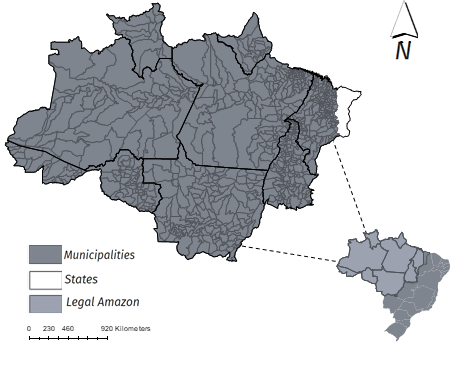
\includegraphics[width=1\textwidth, inner]{Brazil_insect_map_grey.png}
\caption{The Legal Amazon and Municipalities in the 9 states of Brazil: Rond\^{o}nia, Acre, Amazonas, Roraima, Par\'{a}, Amap\'{a}, Tocantins, Maranh\~{a}o e Mato Grosso. Sources: Own construction based on data from \citep{inpe, IBGE1}}.
\label{fig:1}
\end{figure}

The data on deforestation at the municipality level comes from satellite based information from the Brazilian Institute for Space Research \citep{inpe} under the project PRODES and measures yearly deforestation in square kilometers.  The same data also gives us cloud and unobserved areas which represent the area that the satellite could not capture during a certain period. Variables for cloud and no observed areas are used in all regressions to control for measurement error related to the ability of the satellites to detect changes in the land cover across all municipalities. \footnote{According to \citet{kintisch_2007} and \citet{achard_stibig_eva_lindquist_bouvet_arino_mayaux_2010}, the PRODES estimates are considered reliable by the national and international academic science.}

Our dependent variable is the natural log of yearly deforestation within a municipality measured between July and August of any given year. We adjust all numerical variables to match the July-August year.

%beefpricecp
%soypricepp
%woodpricepp
%real gdp

To control for the expansion of commodity markets, we collect soy and wood prices at the municipality level from the Brazilian Statistical Office \citep{IBGE1}.\footnote{Wood prices come from the production of wood defined as firewood and logs of wood in cubic meters.} The beef price is reported at the state level by the Centre for Advanced Studies on Applied Economics \citep{CEPEA}. For municipalities with no data on the commodity markets, we include averaged local prices from neighbouring municipalities weighted by GDP at the municipality level, which differs from previous studies that impute zero prices for all municipalities without production of commodities in order to get the direct effect of commodity price on deforestation of commodities producing regions only \citep{hargrave_kis-katos_2012, LAKES}. We argue this approach by taking into consideration the fact that prices reflect the transport costs from each municipality to neighbouring municipalities and thus not considering averaged neighbouring municipalities price bias downward the results.
%The same procedure is applied to wood price and beef price data. We take this approach because we believe that municipalities with no commodity production still have an implicit price of commodities but this price is not higher enough to incentivise the producers.
All prices are deflated by IPCA which is the official Brazilian consumer price index. GDP is included at the municipality level to control for changes in overall economic activity \citep{IBGE1}. We gather data on federal paved roads since assist commodity activity, and there is an association between road investments and deforestation \citep{PFAFF3, CROPPER1, BAYNARD, pailler_2018}.

%mayor party
%mayor gender
%mayor educ
%mayor age
%env agency
%env law

Data on the institutional environmental framework come from the Survey of Basic Municipal Information \citep{IBGE1}. The data take the form of dummy variables that indicate whether a municipality has an environmental office and has introduced an environmental law. One important aspect that may influence whether a municipality has a well functioning environmental framework is the attitude and character of the local mayor.  Hence, we also collect data from the Survey of Basic Municipal Information on whether the political party of the mayor is pro-farmer in which may be expected to lead to greater deforestation, their education level, gender, age, and  the number of commissioned workers as a proxy for corruption since it is expected that the greater the amount of commissioned workers the higher the rate of deforestation. We also gather data from \citet{TSE} to detect mayor's re-election process. \footnote{More than 20 parties advocate the pro-farmer agenda specially in the Legal Amazon. PMDB (Partido do Movimento Democrático Brasileiro), PP (Partido Progressista), PSDB (Partido da Social Democracia Brasileira) parties respond to almost 44\% of the pro-farmer seats - bancada ruralista in Portuguese - in the deputy chambers. These political parties represent the center-right political spectrum in Brazil with the largest number of affiliates \citep{FPA}.} \footnote{According to the Survey of Basic Municipal Information commissioners workers are employees, who are not effective in the City Hall, and whose only job is the commissioned position they carry out. Usually the position is given by the mayor or city councils in exchange for political favours and benefits which proved to lead to corrupting acts \citep{BUGARIN}.} \footnote{Recently, \citet{pailler_2018} found that deforestation  rates  increased  8–10\%  in  election  years  when  an  incumbent  mayor  ran  for  re-election.}

%PSD (Partido Social Democrático), PR (Partido da Republica), PSB (Partido Socialista Brasileiro), SD (Solidariedade), DEM (Democratas), PTB (Partido Trabalhista Brasileiro), PMB (Partido da Mulher Brasileira), PDT (Partido Democrático Trabalhista), PRB (Partido Republicano Brasileiro), PT (Partido dos Trabalhadores), PSC (Partido Social Cristão), PHS (Partido Humanista da Solidariedade), PV (Partido Verde), PROS (Partido Republicano da Ordem Social), PPS (Partido Popular Socialista), PMN (Partido da Mobilização Nacional), PEN (Partido Ecológico Nacional)

%settlements and housing projects
In terms of other economic and public policies, the number of settlements at municipality level and the settlement density are reported by the Brazilian Agency of Agrarian Reform \citep{incrawebsite2}. We include settlement density to capture rural development in sparse regions.\footnote{Settlement density refers to  number of settled families divided by the area of the settlement.} In addition, we control for the presence of housing projects within a municipality using data from the Survey of Basic Municipal Information \citep{IBGE1}.\footnote{Our housing project dummy is intended to capture a set of interrelated and coordinated actions on housing with the aim of achieving specific objectives such as building houses within the budget limits over a given period of time. "Plano Nacional de Habitação (PlanHab)" and "Minha Casa Minha Vida (MCMV)" in Portuguese are examples of this type of housing projects \citep{Krause2013, KLINTOWITZ2016}.} We also collect data on the extent to which a municipality benefits from subsidised rural credits from the Brazilian central bank \citep{BCB} and development banks \citep{BNB,BASA}. Within the official credit system in each municipality, our rural credit variable is also capturing the amount of credit provided a municipality to encourage agriculture and pasture activities under the economic development policy called National Program for Sustainable Family Agriculture (PRONAF in Portuguese).\footnote{The National Program for Strengthening Family Agriculture (PRONAF) aims to stimulate income generation and improve the family farm production through the financing of rural agricultural and non-agricultural activities and services developed in a rural establishment or in regional communities \citep{PRONAF}.}

%fines, conserv units, rural credits
Finally, we want to control for other environmental related policies that may impact on deforestation rates.  First, we take measure the size of conservation units and the the size of protected indigenous land at municipal level using data from the Brazilian Environmental Ministry \citep{MMMAwebsite}.  Our main environmental policy variable is the sum of these two areas.  We add the values instead of including them separately in our regression analysis because of the high correlation between the two series although we do consider them separately as part of our robustness checks. Second, we collect data on the level of fines imposed at the municipality level for environmental violations provided by the Brazilian Institute of Environment and Renewable Natural Resources \citep{IBAMAwebsite}, so called environmental police.  Fines reflect the amount of money that the agents within a municipality receive as penalization in a given year. In order to get the fines per municipality, we summed all the agents fines for each municipality in any given year. 

Table \ref{tab:summary} provides the summary statistics for our explanatory variables. Table \ref{tab:summary2004} and \ref{tab:summary2015} of the appendix present the summary statistics for the first and last year of our sample analysis and Table \ref{tab:sources} provides the source, level of aggregation and units of measurement for each of our variables.   Overall, note that nearly 45\% of municipalities have an environmental law in place and nearly 75\% have an environmental office. We also find that around 35\% of mayors are over 50 years of age and that nearly 90\% are male. Around 40\% have an education level that is tertiary or above and nearly 2,2\% of the employees in the city hall are commissioned and only 21\% of mayors tend to be re-elected. On average municipalities have 3 settlements within their limits and there are at least 2\% of families living in a settlement. We also verify that on average municipalities have approximately 20 thousands km$^{2}$ of their area protected. We can check that we have R\$3,2 million of fines issued on average per municipality. When examining economic policies we observe that for our sample period the average amount of rural credits per municipality corresponds to R\$20mi and 78\% municipalities have housing projects in place.  

\begin{table}[H]
\footnotesize
    \caption{Summary Statistics - Averages of the sample}
      \begin{tabularx}{\linewidth}{X H H H H}
     \hline
     \hline
      Variable  & Mean & St. Dev. & Min. & \centering\arraybackslash Max.\\
     \hline
    Deforestation   & 20.200 & 57.183 & 0.1 & 1407.8 \\
    Fines &  0.324&    1.298 &  0&    24.227 \\
    Protected Areas  & 2.188 & 5.354 & 0  & 44.877\\
    Rural Credits   &  0.235&    0.948&           0&  22.809\\
    Environmental Law  & 0.450 & 0.497 & 0 & 1 \\
    Environmental Office  & 0.754 & 0.430 & 0 & 1 \\
    Housing Projects   & 0.780 & 0.413 & 0 & 1 \\
    Settlements  & 3.688 & 5.965 & 0 & 76 \\
    Settlements Density  & 0.018 & 0.034 & 0 & 1.016 \\
    GDP  &   0.057 & 0.331 & 0.001 & 9.850 \\
    Beef Price   & 0.852 & 0.472 & 0.518 & 2.419 \\
    Soy Price   &  0.630 & 0.126 & 0.201 & 1.761 \\
    Wood Price   & 0.104 & 0.080 & 0.002 & 0.916 \\
    Roads & 0.019&    0.029&    0.001&    0.089\\
    Clouds &   10.323 & 47.735 & 0 & 1315.286 \\
    No obs &    0.151&    1.507&  0 & 49.786 \\
    Mayor Political Party (pro-farmer)   & 0.920 & 0.271 & 0 & 1 \\
    Mayor Gender (Male)   & 0.901 & 0.298 & 0 & 1 \\
    Mayor Age (\% above 50) &  0.356 & 0.479 & 0 & 1 \\
    Mayor Education &   0.407 & 0.491 & 0 & 1 \\
    Corruption &    0.022 & 0.397 & 0  &   25.167\\
    Re-election &    0.211 & 0.408 & 0  &   1\\
    \hline
    \hline
    \multicolumn{5}{l}{\footnotesize  Note: Statistics refer to N=6178 observations for 562 municipalities for 11 years (2004 - 2015).}
    \end{tabularx}
  \label{tab:summary}
\end{table}
%COLOCAR EXPLICACAO DE FINES

Before describing our empirical strategy we present the trends in deforestation and our key variables over time. Figure \ref{fig:2} shows that according to satellite monitoring, deforestation levels reached their highest levels in 2004 (27,423 square kilometres) \citep{MMMAwebsite}.  Since then there has been a clear decreasing trend. Figure \ref{fig:2} also shows the steady increase in the area of land designated as Protected Areas and the more rapid increase in fines per area of land deforested. We also show the cumulative number of municipalities with environmental law and environmental office which increased steadily with a distinct jump between 2007 and 2008. Similar trends are observed when we compare deforestation rates and changes in the market for commodities that are captured through the price of soy, wood and beef in the Legal Amazon and the institutional environmental framework captured through the existence of environmental law and environmental office in Figure \ref{fig:3}.\footnote{See \citet{hargrave_kis-katos_2012} and \citet{LAKES} for a detailed discussion of the role of commodity markets on deforestation.}

%The analysis of these concerns are the main contribution of this study.

\begin{figure}[H]
  \centering
  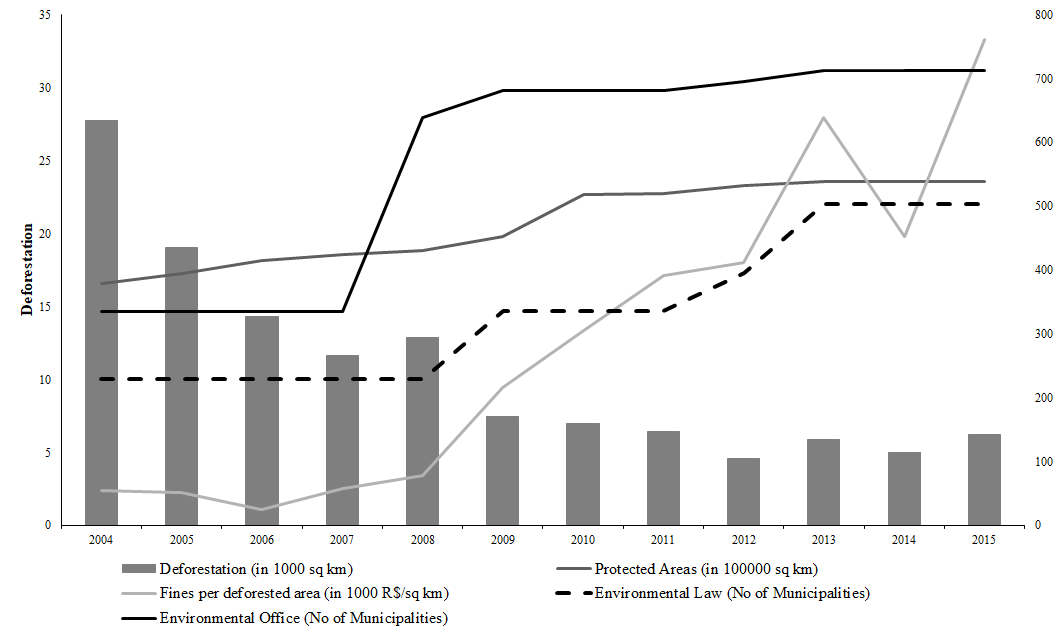
\includegraphics[width=1\textwidth, inner]{Figure1_policy.png}
\caption{Deforestation in the Legal Amazon, Environmental Policy and the Institutional Environmental Framework (2004-2015). Source: \citep{inpe, MMMAwebsite, IBAMAwebsite}}
\label{fig:2}
\end{figure}

\begin{figure}[H]
  \centering
  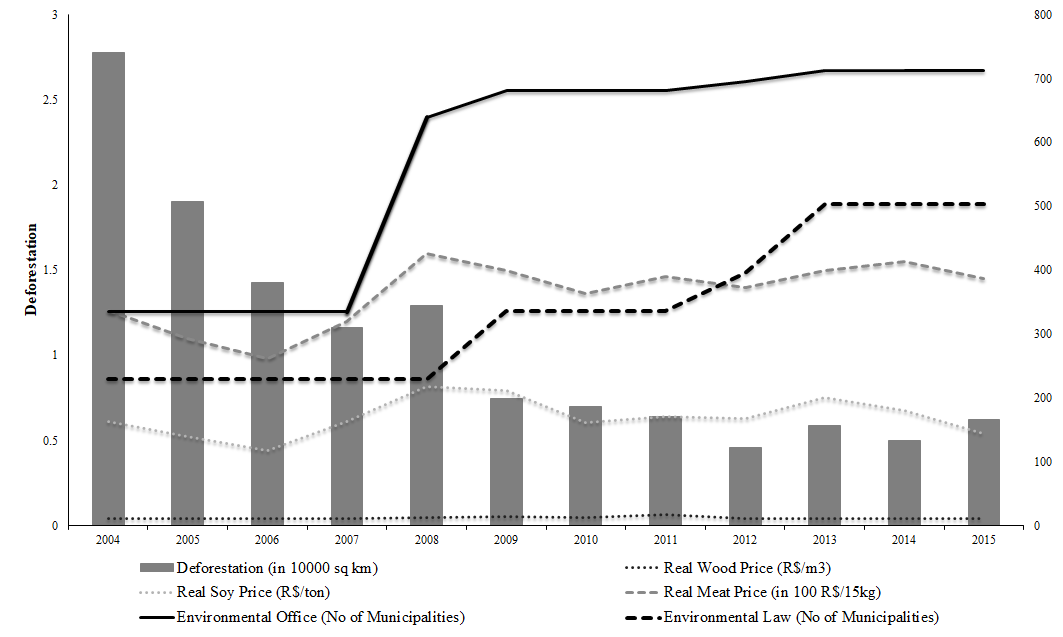
\includegraphics[width=1\textwidth, inner]{Figure1_price.png}
\caption{Deforestation in the Legal Amazon and commodities price the Institutional Environmental Framework (2004-2015). Source: \citep{inpe, IBGE1,CEPEA}}
\label{fig:3}
\end{figure}

%We calculate the intensity of the activity of the environmental police using the real value of fines issued within a municipality divided by deforestation in any given year (see \citet{hargrave_kis-katos_2012}).

\subsection{Empirical strategy}

In order to analyse the impact of different economic and environmental policies and commodity prices under different institutional settings our estimations are based on a panel of municipality level data between 2004 and 2015 which allows us to control for variability across municipalities.  Our baseline regression is given by:

\begin{equation}
    \text{ln}D_{i,t} = \mu_{i} + \text{X}_{i,t-1}\beta_{1}  + \text{X}_{i,t} \beta_{2} + \lambda_{t} + \varepsilon_{i,t} \label{eq:1} \\\\
\end{equation}


where the dependent variable, $lnD_{i,t}$, is the natural log of yearly deforestation in municipality \textit{i} in year \textit{t}. In addition, it includes a fixed parameter of time dummies that capture the effects of overall changes in the explanatory variables in deforestation, $\lambda_{t}$. The vector of controls, $X_{i,t-1}$, includes economic activity (GDP), agricultural prices at municipality level (Soy Price and Wood Price) and state level (Beef Price), access to markets (Roads), the number of settlements within each municipality (Settlements) and number of families per size of settlement (Settlement Density), the total amount of rural credits granted to recipients in a given municipality (Rural Credits) and an indicator variable for the existence of housing projects (Housing Projects) within a municipality, dummy variables to control for political factors (Mayor political party, Mayor education, Mayor gender, Mayor Age), the amount of commissioned workers standardised by population at municipality level (Corruption), and whether the mayor is re-elected or not (Re-election). Our policy variables include fines per municipality in any given year (Fines), the sum of the area of conservational units plus indigenous land per municipality level (Protected Areas). Finally, we include dummy variables for when a municipality has in place either an environmental law and environmental office (with a value of 1 from the year it was in place and zero otherwise.). Finally, we include cloud cover (Clouds) and not observed areas (No obs), $\text{X}_{i,t} \beta_{2}$.

As we are dealing with grouped data, the errors are inter-related and hence we include \citet{DRISCOLL} standard errors that are robust to autocorrelation, heteroskedasticity and cross-sectional dependence. The year and municipality level dummies are included to capture time and municipality invariant effects (e.g. climate, infrastructure or population).

In terms of our right hand side variables in $X_{i,t-1}$, one can conjecture a number of ex-ante expectations of their role in deforestation.  The commodity prices of beef, soy and wood are included to capture the influence of market conditions. For example, if the prices of beef and soy increase, there may be pressure for further deforestation to clear land for cultivation or grazing.  In the case of the price of wood, the effect is ambiguous as on the one hand, as prices rise it may lead to a greater incentive to harvest the forest.  On the other hand, higher prices may lead to a greater awareness of the value of forests and lead to greater efforts to protect what is now a more valuable resource. 
%Another hypothesis bases on the fact that much of Legal Amazon is wood-intensive fuel and increases in the demand for fuel, driven by income growth, induces forest growth as argued by \citet{FOSTER_2003}. 
It is worth to explain that much of deforestation is through illegal logging which we try to capture through market prices. In order to capture access to markets, we include the length of new federal roads and we believe it pressures to further deforestation the more roads and highways are constructed.

Turning to the environmental policies, the expectation is that each policy increases risk of being caught or the cost of transgressing an environmental law which should reduce expected profits associated with deforestation. Hence, we expect a negative sign on the coefficient from our environmental fines variable. The expected sign on our protected areas variable is ambiguous.  On the one hand, if an area is protected in more than name only with additional patrols for example, this should reduce the area in a municipality that can be easily deforested.  On the other hand, the decision to designate an area as protected may have been in response to previous deforestation  as noted by \citet{hargrave_kis-katos_2012} and may capture that deforestation problems are more severe in that particular area. The result of the introduction of a PA might simply be to shift the deforestation activities to areas just outside of the PA but still within a given municipality boundary \citep{GIRARDI}.\footnote{According to \citet{ICMBIO} and \citet{FUNAI} the signalling process of a PA is through signboards. These signboards are implanted in strategic places, that allow to guide the citizen on the access to that area or the transit in the same. Materialising their limits through fences, would have a high cost, which are beyond the resources available for the budget execution of demarcation / georeferencing. There are necessary protection procedures (for herds / planting areas or other protection needs) when requested by the community, but this happens in isolated and specific cases and it is not part of the delimitation of protected areas specifying their physical limits.}

In terms of other public policies we expect housing projects to have a negative impact on deforestation as the provision of affordable housing to inhabitants should reduce the incentive for agents to move to the frontier and clear forest for a place to live. The sign and significance of rural credit variable is uncertain. On the one hand, the availability of official subsidised credit may fuel deforestation by helping to fund clearing through investment in machinery, tools and fertilizers. On the other hand, if credit enables the development of a functioning market in forestry products it may improve forest management practices and reduce deforestation pressures. For our settlement variables, we expect that the number and density of settlements to result in an increase in the demand for deforestation although we expect this relationship to be non-linear hence we include squared terms of each variable.

Finally, our controls for environmental factors which are cloud cover and unobserved areas are expected to have positive and negative coefficients respectively. For unobserved areas, we expect that the greater the area not observed within a municipality, the more difficult it will be to detect the deforestation process. As for cloud cover, the hypothesis is that agents are aware of the policy monitoring program that employs satellite surveillance and may use cloudy days as a cover for their deforesting actions as the satellite may not detect their activity and hence it will reduce their chance of being caught and fined.  Hence, the more cloudy days recorded in a given year is expected to be a positive determinant of deforestation within that year.


%The within transformation removes the fixed municipality-specific effect $\mu_{i}$ and all variables are transformed as deviations from their municipality means. First, we take the average of equation \eqref{eq:1} over time and this gives


%\begin{equation}
%    \text{ln}\overline{D}_{i.} = \mu_{i} + \overline{\text{X}}_{i.}\beta  + \lambda_{t} + %\overline{{\varepsilon}_{i}}  \label{eq:2}
%\end{equation}
						

%Therefore, subtracts the equation \eqref{eq:2} from equation \eqref{eq:1} gives


%\begin{equation}
%	\text{ln}{D}_{i,t} - \text{ln}\overline{D}_{i.} = \beta({\text{X}_{i,t} - \overline{\text{X}}_{i.}}) + %(\varepsilon_{i,t} -  \overline{\varepsilon}_{i.})  \label{eq:3}
%\end{equation}

%Also, averaging across all municipalities in \eqref{eq:1} gives

%\begin{equation}
%    \text{ln}\overline{D}_{..} = \overline{\text{X}}_{..}\beta  + \overline{\varepsilon}_{..}  \label{eq:4}
%\end{equation}
	
%where we already assumed the restriction that the $\sum_{i=1}^{N} \mu_{i} $ = 0  and $\sum_{i=1}^{N} \lambda_{t} $ = 0. This is an arbitrary restriction on the dummy variable coefficients to avoid multicollinearity. In this case, $\widetilde{\beta}$ is obtained from regression \eqref{eq:4}, and the specific effect of each municipality ($\mu_{i}$) and the trend effect ($\lambda_{t}$) can be recovered from

%\begin{equation}
%\widetilde{\mu_{i}} = (\text{ln}\overline{D}_{i.} - \text{ln}\overline{D}_{..}) - %\widetilde{\beta}(\overline{X}_{i.} - \overline{X}_{..}) \label{eq:5}
%\end{equation}

%\begin{equation}
%\widetilde{\lambda_{t}} = (\text{ln}\overline{D}_{.t} - \text{ln}\overline{D}_{..}) - %\widetilde{\beta}(\overline{X}_{.t} - \overline{X}_{..}) \label{eq:6}
%\end{equation}



One of the main contributions of this study is to investigate the interaction between environmental institutions and environmental policies whilst taking into account the expansion in commodity markets captured through commodity prices of beef, wood and soy. Hence, we estimate \eqref{eq:1} given by:





\begin{equation}
\begin{gathered}
\text{ln}D_{i,t} = \mu_{i} + \text{X}_{i,t}\beta_{1} + \text{X}_{i,t-1}\beta_{2}  + \text{(IEF * Env. Policies)}_{i,t-1} \beta_{3} + \\ \text{(IEF * Prices)}_{i,t-1}  \beta_{4} + \lambda_{t} + \varepsilon_{i,t} \label{eq:2} 
\end{gathered}
\end{equation}



so we are able to estimate the extent to which the effectiveness of environmental policies depends on the institutional environmental framework that operates within a municipality. The expectation is that one would observe a reduction in those municipalities that have policies in place that are backed up by proper enforcement of the law through a well functioning institutional framework.  Likewise, in those municipalities the institutional framework is weak then environmental policies may not be introduced, pushed or enforced which would mean an insignificant or even positive effect on overall deforestation rates if loggers are attracted to or pushed from well regulated municipalities. Likewise, combining the institutional environmental framework within a municipality with growth in demand for commodities captured through commodities prices may lead to similar results. One possible driver of the implementation and enforcement of environmental policies are the characteristics and behaviour of the mayor who is in charge of a given municipality. Although we have no priors on age and gender we might expect education to have a negative influence of deforestation while we might expect a mayor that supports pro-farmer policies to have a positive influence on deforestation. The governance attitude of the politicians  within a municipality leading to a corrupted behaviour also has a positive impact on deforestation. Finally, it has been proved that mayors running for re-election tend to explore forests for economic reasons as a way of getting more votes.

One concern with regard to estimating equation \ref{eq:1} and equation \ref{eq:2} is the potential endogeneity of many of the explanatory variables, and hence their interpretation in terms of causality.  Since it would be difficult to find plausible instruments for many, if not for all, of our independent variables, we instead take a three pronged approach to alleviate any such concerns.  First, we control for municipality fixed effects, allowing us to purge all time invariant observables unobservables from the specifications.  Secondly, using an extensive set of other controls, as listed above, we hope to capture all likely determinants of deforestation.  Finally, we lag all control variables by one period, so that under assumption that, after controlling for fixed effects all confounding shocks are only contemporaneous in nature, we are left with solely exogenous variation in the elements of $X_{i,t-1}$.
%COLOCAR AQUI SOBRE IGNORAR ENDOGENEIDADE!!!

%********************************** % Fourth Section  *************************************

\section{Results}
\label{S:4}

\subsection{The effect of environmental policies and market expansion on deforestation}

Results from our estimation of equation \ref{eq:1} are presented in Table \ref{tab:results1}. Our baseline model includes 562 municipalities of the Legal Amazon. In columns (1) through (7) we experiment with including separately environmental policies, such as fines and protected areas, the prices of soy, wood and beef, and our institutional environmental framework variables given by our environmental law and environmental office dummies. Taking our institutional variables first (dummies for an environmental office and an environmental law) we find that neither is significant when included separately in Columns (3) or (4) or together in Column (8). This suggests that having an office and an environmental law in place is necessary but not sufficient to reduce deforestation.

Turning to our other controls, in Column (8) we include all the variables together, our preferred specification.  One immediate observation from Column(8) is that our fines variable is not a significant determinant of deforestation despite the rapid growth in fines levied during this period. One explanation is a lack of enforcement. The environmental police often have limited financial and manpower resources to issue fines but also insufficient legal means for collecting the fines once they have been issued no other way to collect the fine \citep{araujo_barreto_baima_gomes_2017}.  For the PA variable we find an increase in one unit of protected areas (10,000 km$^{2}$) is, ceteris paribus, associated with an increase of 2.7\% in deforestation the following year. To put this number into context we use the mean value of deforestation for our sample (20.2 km$^{2}$) and find out that this percentage would mean average increases in deforestation of 0.55 km$^{2}$.\footnote{It is important to stress that these calculations are only approximations to get an impression about the magnitude of the effect.} One explanation is that PAs are established in response to previous deforestation pressure which is then displaced to neighbouring areas just outside the PAs and is therefore capturing the presence of active groups of loggers in a municipality. In addition, this result might be related to the fact that there are potentially limited public monitoring and enforcement specially in sustainable use PAs in which certain economic activities are allowed \citep{RICO_2017}.\footnote{\citet{RICO_2017} also found a positive result to this relationship when analysing dynamics of forest loss and governance in PA's in the Peruvian Amazon.}

For our market demand variables we find that the estimated coefficient in Column (8) for the price of wood is significant and negative. All other variables remaining constant, an increase in wood price by one unit (1 BRL) leads to an average decrease in deforestation of 128\%. In terms of our sample, this percentage would mean average decreases in deforestation of approximately 26km$^{2}$. The coefficients on the price of beef and soy are not significant either together or individually.

In terms of our other economic policy variables, we find that the greater the number of settlements within a municipality the greater the degree of deforestation (a positive liner term) but at a decreasing rate (a negative squared term). Increasing the number of settlements will lead to, ceteris paribus, an increase in deforestation by nearly 6\%. The turning point is inside the sample range. We estimate the turning point to be 16 settlements within a municipality and from our sample we know that only five percent of our municipalities sample have passed the turning point which suggests that for the vast majority of municipalities additional settlements lead to increased deforestation.\footnote{Concei\c{c}\~{a}o do Araguaia - Par\'{a}, Itupiranga - Par\'{a}, Marab\'{a} - Par\'{a}, Novo Repartimento - Par\'{a} and Z\'{e} Doca - Maranh\~{a}o represent the municipalities with the highest number of settlements.} 

For our settlement density variable we find that increasing density settlements within a municipality leads to higher deforestation but that the effect is non-linear so that deforestation increases but at a decreasing rate. More densely populated settlements deforest more within a municipality as pressure on land and the need for expansion is greater. The high density turning point which is 0.62 includes only one settlement called Altamira in Para and is more developed economically leading to less pressure to deforest for economic purposes. Increasing the number of families per settlement within a municipality is associated with increasing deforestation at a decreasing rate of 280\%. Likewise, housing projects have a negative effect on deforestation as expected, since reduces the incentive for agents living in poor quality housing clear land to live. The estimated coefficient implies that the existence of housing projects within a municipality decreases logged deforestation by 15\%. To put this number into context, we use the mean value of deforestation for our sample (20.2 km$^{2}$) and detect that represents average decreases in deforestation of 3 km$^{2}$.

Turning to the political factors, we notice that only mayor age and corruption have a significant effect on deforestation. We find that an increase in age above the average (50 years) results in an average decrease in deforestation of 5.6$\%$. At the mean value of deforestation for our sample, we understand that this small fraction would represent an average decrease in deforested areas of 1.1km$^{2}$. The justification relies on the argument that younger politicians that want to stay in power for longer periods are more prone to undertake incentives that contradict the environmental agenda, while older politicians tend to be more experienced and cautious in dealing with environmental agendas. Corruption, mirrored in the number of commissioned workers per population, leads to higher deforestation within a municipality. In essence, an increase in number of commissioned workers per population by one unit  is associated with an increase of 2.4\% in deforestation. For our sample, this would represent an increase of 0.48 km$^{2}$ per each additional commissioned worker averaged by population. It is of interest to observe that corruption is positive and significant in columns (1) through (8), which endorses the necessity of this political control. Gender, being a pro-farmer politician, and having an education level of tertiary of above have no effect on deforestation rates.

\begin{table}[htp!]
\caption{Effects of Environmental Policies and Commodities Prices on Deforestation}
\scriptsize
       \begin{tabularx}{\columnwidth}{Z E E E E E E E E }
       \hline
     \hline
      Sample & \multicolumn{5}{l}{Dependent: $\Delta$ \textit{ln} Deforestation} \\ \cline{2-9}
      & (1) & (2) & (3) & (4) & (5) & (6) & (7) & (8) \\
        \hline
    Sett$_{-1}$ & 0.080***	&	0.070***	&	0.078***	&	0.079***	&	0.074***	&	0.079***	&	0.078***	&	0.064***\\
	                   & 	(5.36)	&	(4.59)	&	(5.61)	&	(5.50)	&	(4.87)	&	(5.50)	&	(5.08)	&	(3.98)	\\
    Sett$_{-1}$ sq & -0.002**	& -0.002**	& -0.002***	& -0.002***	&	-0.002**	&	-0.002**	&	-0.002**	&	-0.002**	\\
                        & 			(3.04)	&	(2.90)	&	(3.16)	&	(3.18)	&	(2.97)	&	(2.94)	&	(3.08)	&	(2.48)	\\
    Sett Dens$_{-1}$ & 4.056**	&	4.510***	&	4.159**	&	4.120**	&	3.866**	&	4.397***	&	4.116**	&	4.685***	\\
                        & 		(2.99)	&	(3.36)	&	(2.89)	&	(2.97)	&	(2.97)	&	(3.13)	&	(2.92)	&	(3.73)	\\
    Sett Dens$_{-1}$ sq & -3.639***	&	-3.212**	&	-3.620***	&	-3.581***	&	-3.283***	&	-3.841***	&	-3.581***	&	-3.353***	\\
                        & 	(3.51)	&	(2.88)	&	(3.41)	&	(3.50)	&	(3.60)	&	(3.70)	&	(3.47)	&	(3.34)	\\
    Rural Credits$_{-1}$ & 0.025	&	0.025*	&	0.024	&	0.024	&	0.024	&	0.024	&	0.028	&	0.028	\\
                        & 		(1.75)	&	(1.81)	&	(1.77)	&	(1.77)	&	(1.71)	&	(1.67)	&	(1.61)	&	(1.51)	\\
    Housing Projects$_{-1}$ & -0.147**	&	-0.150**	&	-0.147**	&	-0.147**	&	-0.150**	&	-0.147**	&	-0.149**	&	-0.153**	\\
                        & 		(2.92)	&	(2.83)	&	(2.91)	&	(2.92)	&	(2.91)	&	(2.93)	&	(2.80)	&	(2.71)	\\
    GDP$_{-1}$ & -0.237	&	-0.249	&	-0.234	&	-0.248	&	-0.232	&	-0.261	&	-0.232	&	-0.274	\\
                        & 	(1.50)	&	(1.56)	&	(1.46)	&	(1.53)	&	(1.50)	&	(1.60)	&	(1.52)	&	(1.66)	\\
    GDP$_{-1}$ sq & 0.027	&	0.028	&	0.027	&	0.027	&	0.025	&	0.031	&	0.026	&	0.031	\\
                        & 		(1.48)	&	(1.51)	&	(1.46)	&	(1.49)	&	(1.48)	&	(1.68)	&	(1.51)	&	(1.74)	\\
    Mayor Party$_{-1}$ & 0.041	&	0.039	&	0.039	&	0.042	&	0.037	&	0.039	&	0.042	&	0.036	\\
                        & 		(0.90)	&	(0.86)	&	(0.86)	&	(0.93)	&	(0.85)	&	(0.87)	&	(0.89)	&	(0.81)	\\
    Mayor Education$_{-1}$ &	0.010	&	0.016	&	0.011	&	0.011	&	0.012	&	0.019	&	0.011	&	0.024	\\
                        & 		(0.31)	&	(0.57)	&	(0.35)	&	(0.38)	&	(0.41)	&	(0.68)	&	(0.38)	&	(0.96)	\\
    Mayor Age$_{-1}$ & -0.065**	&	-0.062**	&	-0.063**	&	-0.064**	&	-0.060**	&	-0.062**	&	-0.060**	&	-0.056**	\\
                        & 		(2.46)	&	(2.38)	&	(2.40)	&	(2.46)	&	(2.41)	&	(2.29)	&	(2.61)	&	(2.39)	\\
    Mayor Gender$_{-1}$ &	0.025	&	0.025	&	0.023	&	0.021	&	0.020	&	0.030	&	0.022	&	0.030	\\
                        & 		(0.69)	&	(0.66)	&	(0.61)	&	(0.55)	&	(0.53)	&	(0.79)	&	(0.58)	&	(0.78)	\\
    Corruption$_{-1}$ & 0.026**	&	0.026**	&	0.026**	&	0.025**	&	0.026**	&	0.026**	&	0.025**	&	0.024**	\\
                        & 		(2.94)	&	(2.98)	&	(2.78)	&	(2.78)	&	(2.85)	&	(2.88)	&	(2.70)	&	(2.90)	\\
    Re-election$_{-1}$ &	0.004	&	0.002	&	0.003	&	0.003	&	-0.004	&	0.003	&	-0.000	&	-0.008	\\
    	                & (0.17)	&	(0.11)	&	(0.14)	&	(0.14)	&	(0.21)	&	(0.11)	&	(0.01)	&	(0.35)	\\
    Roads$_{-1}$ & -0.614	&	1.218	&	-0.954	&	-0.697	&	1.134	&	-0.646	&	-5.817	&	-2.007	\\
                        &  	(0.08)	&	(0.15)	&	(0.12)	&	(0.09)	&	(0.17)	&	(0.08)	&	(0.34)	&	(0.15)	\\              
    Clouds & 0.001	&	0.000	&	0.001	&	0.001	&	0.001	&	0.001	&	0.001	&	0.000	\\
                        & 	(0.61)	&	(0.47)	&	(0.60)	&	(0.59)	&	(0.63)	&	(0.59)	&	(0.61)	&	(0.47)	\\
    NoObs & 	-0.004	&	-0.002	&	-0.004	&	-0.003	&	-0.003	&	-0.003	&	-0.003	&	0.000	\\
                      	& (0.47)	&	(0.25)	&	(0.50)	&	(0.42)	&	(0.37)	&	(0.41)	&	(0.42)	&	(0.09)	\\
    Fines$_{-1}$ & 	-0.015	&		&		&		&		&		&		&	-0.018	\\
                        & 		(0.73)	&		&		&		&		&		&		&	(0.83)	\\
    PAs$_{-1}$ & 		&	0.027***	&		&		&		&		&		&	0.027***	\\
                        &  &	(4.10)	&		&		&		&		&		&	(3.89)	\\
    Env. Law$_{-1}$ & 		&		&	0.022	&		&		&		&		&	0.022	\\
                        & 			&		&	(0.95)	&		&		&		&		&	(1.00)	\\
    Env. Office$_{-1}$ &		&		&		&	-0.054	&		&		&		&	-0.058	\\
                        & 			&		&		&	(1.55)	&		&		&		&	(1.51)	\\
    Soy Price$_{-1}$  & 	&		&		&		&	0.630	&		&		&	0.549	\\
                        & 			&		&		&		&	(1.27)	&		&		&	(1.18)	\\
    Wood Price$_{-1}$  & 	&		&		&		&		&	-1.331*	&		&	-1.285*	\\
                        & 		&		&		&		&		&	(2.02)	&		&	(2.11)	\\
    Beef Price$_{-1}$  & 		&		&		&		&		&		&	1.664	&	1.180	\\
                        & 		&		&		&		&		&		&	(0.58)	&	(0.49)	\\
    \hline
    %Other Set of Controls &  Yes & Yes & Yes & Yes \\
    Year Fixed Effects &   Yes & Yes & Yes & Yes & Yes & Yes & Yes & Yes \\
    Municipality Fixed Effects &   Yes & Yes & Yes & Yes & Yes & Yes & Yes & Yes \\
    Number of Observations &   6,178 &   6,178 &   6,178 &   6,178 &   6,178 &   6,178 &   6,178 &   6,178\\
    \hline 
    \hline
    \multicolumn{9}{l}{*, **, *** denote significance at 10$\%$, 5$\%$ and 1$\%$ levels, respectively. Robust standard error values are }\\
    \multicolumn{9}{l}{indicated in parentheses under the coefficients.  PAs stand for Protected Areas.}\\
\end{tabularx}
\label{tab:results1}
\end{table}

\subsection{Environmental policies and market expansion conditioning on institutional environmental framework}
\label{SS:4.1}

In Table \ref{tab:results2} we consider the impact of our policy variables and commodities prices conditional on the institutional environmental framework with the same set of controls from Table \ref{tab:results1} and the year fixed effects (Columns 1-8). In Column 9 we show that agents from municipalities that receive fines when there is an environmental law in place does not reduce deforestation. One explanation is that in the Legal Amazon many local environmental laws are not enforced following environmental incidents even though the municipalities have the power to do so. Thus, it seems more likely that the offender will be punished at the state or federal level rather than at the municipality level, which contributes to the limited effectiveness of fines as a punitive instrument at the local level.

In contrast, we find that there is a significant drop in deforestation through a policy of fines if an environmental office exists. More specifically, the estimated average drop in deforestation associated with the fines policy when there is a municipality with an environmental office is around 1.8 km$^{2}$ ceteris paribus. This finding illustrates that the coordinated process of implementation of the national environmental system (SISNAMA) that decentralises forces to assist the protection of the environment can have a positive effect curbing deforestation. Environmental offices appear to act as a primary partner to the SISNAMA together with IBAMA, which operates at the national level as an administrative arm and environmental police of the Brazilian Ministry of Environment. This coalition appears to make the institutional framework work more effectively at the local level. 

We also find that municipalities with an environmental office and protected areas within their territory tend to increase deforestation by approximately 3\%. Using the mean value of deforestation for our sample (20.2 km$^{2}$) we detect that this percentage represents average increases in deforestation of 0.6 km$^{2}$. This unexpected result may be because environmental offices are often set up to work together with other offices, such as agriculture, tourism, education, and infrastructure offices. In this sense environmental management is often associated with other themes and the creation of joint offices can lead to conflict with the agendas of others. For example, given that expansion of agriculture is an important factor in deforestation, having a joint office of environment and agriculture could lead to a conflict of interest. Regarding protected areas, conditioned on environmental laws at the municipality level, we find no significant effect.  This suggests that protected areas are not entirely monitored at the local level since a substantial number of these units are regulated at the state and federal level. 

Turning to our commodity market variables, we find that the institutional environmental framework plays an important role when conditioned on commodity prices. Soy prices conditioned on the existence of environmental law correspond to averages decreases of deforestation of almost 73\%. Arguably much of this effect is likely to be the result of the moratorium implemented in 2006.\footnote{The moratorium establishes that companies purchasing the grain and its derivatives can not acquire from those who produced in deforested areas after 2008, within indigenous lands or that are on the slave labour list. The moratorium instrument prohibited soy producers from negotiating the sale of production originating from deforested areas in the legal Amazon for a period of two years.}  In this sense, the institutional environmental framework was used to help compliance with the soy moratorium. However, when looking to the overall effect we can observe that soy price influence deforestation positively. An increase in soy price by one unit (1 BRL) at mean values for the existence of environmental law is, ceteris paribus, associated with an average increase in deforestation of approximately 46\%. We find no significant effect for other commodities when conditioning on the existence of an environmental law. \footnote{Recently, \citet{CAVIGLIAHARRIS2018232} addressed the existence of a nonlinear relationship with the intensification of cattle production in part of the Legal Amazon. First as farms become more intensive the demand for newly cleared land increases, but then decreases with further intensification.}

In contrast, wood (negative) and beef (positive) prices are significant when conditioned on environmental office. This is consistent with our assumptions that environmental management offices are associated with other strategic themes and that a institutional framework on its own fails to protect the environment. From our sample, forestry prices have a negative impact on deforestation and beef market has a positive impact on deforestation. Taking the mean value of deforestation (20.2 km$^{2}$) we find out that forestry prices would produce average decreases in deforestation of 38 km$^{2}$ and for the beef market we would see average increases in deforestation of 1.4 km$^{2}$.

\begin{landscape}
\begin{table}[htpb!]
\caption{Effects of Environmental Policies on Deforestation: Baseline Model}
\scriptsize
\begin{tabularx}{0.82\linewidth}{l Z Z Z Z Z Z Z Z Z}
     \hline
     \hline
      Sample & \multicolumn{9}{l}{Dependent: $\Delta$ \textit{ln} Deforestation} \\ \cline{2-10}
      & (1) & (2) & (3) & (4) & (5) & (6) & (7) & (8) & (9) \\
        \hline
        
    %%%%%%%%%%%%%%%%%%%%%%%%%%%%%%%%%%%%%%%%%%%%%%%%%%%%%%%%%%%%%%%%%%%%%%%%
    %%%%%%%%%%%%%%%%%%%%%%%%%%%%%%%%%%%%%%%%%%%%%%%%%%%%%%%%%%%%%%%%%%%%%%%%
    %%%%%%%%%%%%%FALTA ATUALIZAR OS DADOS EM VERDE%%%%%%%%%%%%%%%%%%%%%%%%%%
    %%%%%%%%%%%%%%%%%%%%%%%%%%%%%%%%%%%%%%%%%%%%%%%%%%%%%%%%%%%%%%%%%%%%%%%%
    %%%%%%%%%%%%%%%%%%%%%%%%%%%%%%%%%%%%%%%%%%%%%%%%%%%%%%%%%%%%%%%%%%%%%%%%
    
    %Settlements$_{-1}$ & 0.064***	&	0.060***	&	0.063***	&	0.065***	&	0.064***	&	0.060*** &	0.061***&	0.063***	&	0.062***\\
    %                    & 	(3.71)	&	(3.66)	&	(4.12)	&	(4.17)	&	(3.99)	&	(3.48)	&	(3.64)	&	(3.86)	&	(3.79)\\
    %Settlements$_{-1}$ sq & -0.001*	&	-0.001*	&	-0.001**	&	-0.001*	&	-0.001**	&	-0.001*	&	-0.001*	&	-0.001*	&	-0.001**\\
    %                    & 		(2.05)	&	(2.10)	&	(2.21)	&	(2.17)	&	(2.21)	&	(2.00)	&	(2.04)	&	(2.04)	&	(2.01)\\
    %Settlements Dens$_{-1}$ & 4.568***	&	4.653***	&	4.583***	&	4.765***	&	4.511*** &	4.640*** &	4.640*** &	4.806***	&	4.772***\\
    %                    & 	(3.76)	&	(3.94)	&	(3.72)	&	(3.93)	&	(3.66)	&	(3.97)	&	(3.95)	&	(4.11)	&	(4.09)\\
    %Settlements Dens$_{-1}$ sq & -3.712***	&	-3.639***	&	-3.694***	&	-3.820*** &	-3.653*** &	-3.667*** &	-3.673*** &	-3.790***	&	-3.769***\\
    %                    & 	(3.96)	&	(4.16)	&	(3.84)	&	(4.11)	&	(3.86)	&	(4.24)	&	(4.18)	&	(4.32)	&	(4.30)\\
    %Rural Credits$_{-1}$ & 1.948	&	1.589	&	1.587	&	1.823	&	1.732	&	1.803	&	1.642	&	1.672	&	1.664\\
    %                    & 	(1.31)	&	(1.07)	&	(1.08)	&	(1.21)	&	(1.13)	&	(1.25)	&	(1.16)	&	(1.20)	&	(1.20)\\
    %Housing Projects$_{-1}$ & -0.142**	& -0.147** &	-0.138**	&	-0.133**	&	-0.143** & -0.146**	&	-0.141**	&	-0.131**	&	-0.131**\\
    %                    & 	(2.55)	&	(2.73)	&	(2.56)	&	(2.51)	&	(2.56)	&	(2.72)	&	(2.72)	&	(2.66)	&	(2.65)\\
    %GDP$_{-1}$ & -0.214	&	-0.231	&	-0.204	&	-0.225	&	-0.221	&	-0.230	&	-0.220	&	-0.229	&	-0.226\\
    %                   &  (1.43)	&	(1.53)	&	(1.23)	&	(1.57)	&	(1.46)	&	(1.51)	&	(1.29)	&	(1.38)	&	(1.39)\\
    %GDP$_{-1}$ sq & 0.026	&	0.027	&	0.026	&	0.028*	&	0.026	&	0.027	&	0.027	&	0.029	&	0.029\\
    %                    & 	(1.60)	&	(1.67)	&	(1.50)	&	(1.80)	&	(1.64)	&	(1.64)	&	(1.51)	&	(1.65)	&	(1.66)\\
    %Mayor Party$_{-1}$ & 0.042	&	0.040	&	0.048	&	0.041	&	0.045	&	0.038	&	0.043	&	0.042	&	0.042\\
    %                   & 	(0.95)	&	(0.92)	&	(1.09)	&	(0.94)	&	(1.03)	&	(0.88)	&	(0.97)	&	(0.95)	&	(0.95)\\
    %Mayor Education$_{-1}$ & 0.013	&	0.022	&	0.013	&	0.016	&	0.017	&	0.019	&	0.015	&	0.014	&	0.015\\
    %                    & 	(0.50)	&	(0.84)	&	(0.48)	&	(0.59)	&	(0.63)	&	(0.73)	&	(0.59)	&	(0.56)	&	(0.58)\\
    %Mayor Age$_{-1}$ & -0.060**	&	-0.057*	&	-0.058**	&	-0.059**	&	-0.060**	&	-0.056*	&	-0.053*	&	-0.053*	&	-0.052*\\
    %                   & 	(2.39)	&	(2.20)	&	(2.30)	&	(2.33)	&	(2.43)	&	(2.17)	&	(2.03)	&	(1.97)	&	(1.97)\\
    %Mayor Gender$_{-1}$ & 	0.026	&	0.027	&	0.029	&	0.029	&	0.031	&	0.024	&	0.023	&	0.024	&	0.024\\
    %                    & 	(0.65)	&	(0.68)	&	(0.71)	&	(0.72)	&	(0.78)	&	(0.60)	&	(0.59)	&	(0.60)	&	(0.61)\\
    %Corruption$_{-1}$ & 0.026***	&	0.026***	&	0.026***	&	0.025***	&	0.025**	&	0.026***	&	0.026*** & 0.026***	&	0.026***\\
    %                   & (3.26)	&	(3.22)	&	(3.76)	&	(3.19)	&	(3.10)	&	(3.35)	&	(4.02)	&	(4.07)	&	(4.06)\\
    %Roads$_{-1}$ & -0.106	&	0.971	&	2.265	&	2.292	&	-0.337	&	0.750	&	3.055	&	5.021	&	4.060\\
    %                   & 	(0.01)	&	(0.08)	&	(0.18)	&	(0.17)	&	(0.03)	&	(0.06)	&	(0.24)	&	(0.38)	&	(0.30)\\
    %Clouds$_{-1}$ & 0.013**	&	0.013**	&	0.014**	&	0.012**	&	0.013**	&	0.013**	&	0.013**	&	0.012**	&	0.012**\\
    %                    & 	(2.50)	&	(2.76)	&	(2.83)	&	(2.53)	&	(2.85)	&	(2.47)	&	(2.47)	&	(2.26)	&	(2.25)\\
    %Forest$_{-1}$ & 0.020*	&	0.022**	&	0.022**	&	0.019*	&	0.021**	&	0.020*	&	0.020*	&	0.018*	&	0.018*\\
    %                    & 	(2.19)	&	(2.48)	&	(2.53)	&	(2.19)	&	(2.55)	&	(2.18)	&	(2.18)	&	(1.96)	&	(1.95)\\
    Fines$_{-1}$ & 0.079	&	-0.019	&	-0.018	&	-0.017	&	-0.018	&	0.080*	&	0.083*	&	0.069	&	0.069	\\
                        & 	(1.73)	&	(0.89)	&	(0.84)	&	(0.80)	&	(0.84)	&	(1.82)	&	(1.90)	&	(1.64)	&	(1.62)	\\
    Protected Areas$_{-1}$ & 0.027***	&	-0.004	&	0.026***	&	0.026***	&	0.027***	&	-0.004	&	-0.005	&	-0.003	&	-0.003	\\
                        & 		(3.99)	&	(0.38)	&	(3.73)	&	(3.79)	&	(3.91)	&	(0.35)	&	(0.43)	&	(0.30)	&	(0.30)	\\
    Env. Law$_{-1}$ &	0.024	&	0.008	&	0.478***	&	0.079*	&	0.072*	&	0.010	&	0.470***	&	0.532***	&	0.538***	\\
                        & 	(1.04)	&	(0.36)	&	(3.38)	&	(2.12)	&	(2.19)	&	(0.39)	&	(3.27)	&	(3.18)	&	(3.22)	\\
    Env. Office$_{-1}$ & -0.041	&	-0.094*	&	0.122	&	0.131**	&	-0.101	&	-0.077	&	0.125	&	0.293	&	0.287	\\
                        & 	(1.03)	&	(2.06)	&	(0.63)	&	(2.38)	&	(1.27)	&	(1.61)	&	(0.63)	&	(1.45)	&	(1.45)	\\
    Soy Price$_{-1}$  & 0.551	&	0.558	&	1.068**	&	0.553	&	0.549	&	0.561	&	1.109***	&	1.114***	&	1.188**	\\
                        & 	(1.17)	&	(1.21)	&	(3.06)	&	(1.20)	&	(1.18)	&	(1.21)	&	(3.20)	&	(3.12)	&	(3.10)	\\
    Wood Price$_{-1}$  & -1.263*	&	-1.282*	&	-1.294*	&	0.855	&	-1.280*	&	-1.261*	&	-1.270*	&	0.686	&	0.639	\\
                        & 	(2.08)	&	(2.19)	&	(2.12)	&	(1.13)	&	(2.11)	&	(2.16)	&	(2.17)	&	(0.90)	&	(0.81)	\\
    Beef Price$_{-1}$  & 	1.089	&	1.109	&	1.232	&	0.791	&	1.200	&	1.014	&	1.060	&	0.723	&	0.685	\\
                        & 	(0.44)	&	(0.47)	&	(0.53)	&	(0.33)	&	(0.50)	&	(0.42)	&	(0.46)	&	(0.31)	&	(0.29)	\\
    Env. Law$_{-1}$* Fines$_{-1}$ & -0.009	&		&		&		&		&	-0.012	&	-0.014	&	-0.012	&	-0.012	\\
                        & 		(0.47)	&		&		&		&		&	(0.71)	&	(0.91)	&	(0.74)	&	(0.73)	\\
    Env. Office$_{-1}$* Fines$_{-1}$& -0.101**	&		&		&		&		&	-0.101***	&	-0.103***	&	-0.089**	&	-0.088**	\\
                        & (3.03)	&		&		&		&		&	(3.12)	&	(3.18)	&	(2.79)	&	(2.77)	\\
    Env. Law$_{-1}$* PAs$_{-1}$ &	&	0.007	&		&		&		&	0.008	&	0.008	&	0.007	&	0.007	\\
                        & 				&	(1.29)	&		&		&		&	(1.44)	&	(1.50)	&	(1.40)	&	(1.38)	\\
    Env. Office$_{-1}$* PAs$_{-1}$& 		&	0.029**	&		&		&		&	0.029**	&	0.029**	&	0.028**	&	0.028**	\\
                        & 		&	(2.95)	&		&		&		&	(2.94)	&	(2.93)	&	(2.82)	&	(2.83)	\\
    Env. Law$_{-1}$* Soy Price$_{-1}$  &  	&		&	-0.716***	&		&		&		&	-0.721***	&	-0.736***	&	-0.729***	\\
                        & 			&		&	(3.55)	&		&		&		&	(3.40)	&	(3.47)	&	(3.16)	\\
    Env. Office$_{-1}$* Soy Price$_{-1}$& 		&		&	-0.308	&		&		&		&	-0.346	&	-0.339	&	-0.447*	\\
                        &  			&					&	(1.09)	&		&		&		&	(1.21)	&	(1.25)	&	(1.90)	\\
    Env. Law$_{-1}$* Wood Price$_{-1}$&  	&		&		&	-0.483*	&		&		&		&	-0.442	&	-0.450	\\
                        &  				&		&		&	(2.19)	&		&		&		&	(1.65)	&	(1.69)	\\
    Env. Office$_{-1}$* Wood Price$_{-1}$ & 	&		&		&	-2.120***	&		&		&		&	-1.941***	&	-1.891***	\\
                        &  				&		&		&	(6.92)	&		&		&		&	(5.67)	&	(5.35)	\\
    Env. Law$_{-1}$* Beef Price$_{-1}$& 	&		&		&		&	-0.060**	&		&		&		&	-0.011	\\
                        &  				&		&		&		&	(2.54)	&		&		&		&	(0.50)	\\
    Env. Office$_{-1}$* Beef Price$_{-1}$ &		&		&		&		&	0.049	&		&		&		&	0.070**	\\
                        &  			&		&		&		&	(1.26)	&		&		&		&	(2.26)	\\
    \hline
    Set of Controls &   Yes & Yes & Yes & Yes & Yes & Yes & Yes & Yes & Yes \\
    Year Fixed Effects &   Yes & Yes & Yes & Yes & Yes & Yes & Yes & Yes & Yes \\
    Municipality Fixed Effects &   Yes & Yes & Yes & Yes & Yes & Yes & Yes & Yes & Yes \\
    Number of Observations &   6,178 &   6,178 &   6,178 &   6,178 &   6,178 &   6,178 &   6,178 &   6,178 &   6,178\\
    \hline
    \hline
    \multicolumn{10}{l}{ *, **, *** denote significance at 10$\%$, 5$\%$ and 1$\%$ levels, respectively. Robust standard error values are indicated in parentheses under the coefficients. PAs }\\
    \multicolumn{10}{l}{stand for Protected Areas.}\\
    \end{tabularx}%
  \label{tab:results2}%
\end{table}%
\end{landscape}

\subsection{Spatial Analysis}
\label{SS:4.2}

It is possible that deforestation has a spatial dependence i.e. deforestation process affects neighbouring municipalities and when there is a strong institutional environment there is a possibility to shift deforestation to municipalities with low enforcement. In order to check this assumption, we conduct a spatial analysis of spatial dependence following \citet{ANSELIN} and \citet{elhorst_2012}. The existence of spatial autocorrelation can occur if a given event in a given place has a significant impact on neighbouring regions. Spatial dependence relates to the idea of relative location and the interdependence between regions and the spillover effects of certain activities or factors and that interdependence may affect both the characteristics of the data and the nature of the events. Spatial econometric models with panel data capture the relationship between variables over time and arising for the existence for spatial autocorrelation. It should be added that it is assumed that the area studied remains constant over the period of years \citep{ALMEIDA}. 
For this analysis, we needed a strong balanced panel, so our sample reduced from 562 to 456 which is still represents 65\% of total Legal Amazon municipalities. We performed LM tests to establish the dependence factor (see Table \ref{tab:LMtests}). Up to this point, the test results pointed to the spatial lag model specification. In view of testing procedure we ran the two models, spatial auto-regressive model (SAR), spatial error model (SEM) (not shown here) and SAR is preferred to SEM in all specifications. 

To incorporate the autocorrelation of spatial lag type of dependent variable, our fixed effects model needs to be modified, generating the Spatial Autoregressive model with fixed effects:


\begin{equation}
\begin{gathered}
\text{ln}D_{i,t} = \mu_{i} + \rho W_{1}y_{t} +  \text{X}_{i,t}\beta_{1} + \text{X}_{i,t-1}\beta_{2}  + \text{(IEF * Env. Policies)}_{i,t-1} \beta_{3} + \\ \text{(IEF * Prices)}_{i,t-1}  \beta_{4} + \lambda_{t} + \varepsilon_{i,t} \label{eq:2} 
\end{gathered}
\end{equation}

where $W_{1}y_{t}$ is the spatial lag of the dependent variable. The spatial weight matrix W is defined according to various criteria and is maintained unchanged for all years of the panel. The calculation of the spatial weight matrices used the coordinates from the municipality's centroid. We calculated three different weight matrices. Our baseline weight matrix (W1) finds the 5 nearest neighbours and constructs a spatial weight matrix based on this number of neighbours, normalised to have row-sums of unity. Alternatively, we create a distance based spatial weight matrix (W2) with bands using latitude and longitude coordinates a the Great Circle distance formula. The bands used were 1km to 100km. Finally, we construct a distance based spatial weight matrix (W3) using latitude and longitude coordinates and the Great Circle distance formula (Lacombe's Method) \citep{elhorst_2012}. Using these techniques we gradually increase the number of neighbours.

Since it is not possible to compare the coefficient estimates in the non-spatial model, our baseline, with their counterparts in the spatial models SAR, we use the direct and indirect effects estimates as a result of impacts passing through neighbouring municipalities and back to the municipalities themselves. These feedback effects are partly due to the coefficient of the spatially lagged dependent variable. Within this perspective, we follow \cite{lesage_pace_2009} and present he direct, indirect and total effect of the coefficients separately.

Table \ref{tab:spatialW} report our results for the three different matrices. All results are consistent with the literature \citep{LAMBIN1, LAMBIN2}. We first consider the direct effect of our estimates. We can see that one of the institutional apparatus - environmental law - has no direct effect when conditioning on protected areas and, wood and beef commodities. Our spatial correlation is positive and significant and can be interpreted as the impact of changes in municipality on deforestation. The impact would be magnified by 1.2 and 1.6 through the spatial lag in the model. For our baseline weight matrix (W), we can see that the direct effect of Fines, from the SAR model, on deforestation was underestimated by a factor of 0.75. Since the direct effect of Fines is 0.517 and its coefficient estimate 0.596, its feedback effect
amounts to 0.07 or 15\% of the direct effect. In other words, these feedback effects turn out to be relatively reasonable. For environmental law and office using the second approach of weights we account that their effect amounts to 0.24 and 0.15 or 79\% and 14\% of the direct effect respectively. Looking to the indirect effect on the third model (W3), we can clearly see that the indirect effect of a change in the amount of fines issued appears to be 62\% of the direct effect. If the amount of fines issued increase in one municipality, the change in neighbouring municipalities to the change in the municipality itself is in the proportion of approximately 1 to 1.6 in case of increasing Fines. 

Overall, we can observe that the Institutional Environmental Framework (IEF) when established in a municipality tend to detain deforestation in neighbouring municipalities. As an example, in all of our specifications conditioning the existence of the IEF and the exercise of fines we have a negative effect on neighbouring municipalities. We can see the same effect for the market expansion conditioned on the IEF which corroborates with our main findings \ref{tab:results2}. 

\begin{table}[htpb!]
\caption{Spatial Analysis - Baseline Model}
\scriptsize
       \begin{tabularx}{0.8\linewidth}{E C C C}
     \hline
        \multicolumn{4}{l}{Dependent: $\Delta$ \textit{ln} Deforestation}\\ \cline{1-4}
    Sample & W1 & W2 & W3 \\
        \hline
    Fines$_{-1}$ &	0.596	(10.549) &	0.595 (10.532) &	0.599	(10.742)\\
    Protected Areas$_{-1}$ &	-0.025	(-1.891)&	-0.025 (-1.890) &	-0.030	(-2.281) \\
    Env. Law$_{-1}$ &	0.542	(2.369) &	0.543 (2.375) &	0.578	(2.560) \\
    Env. Office$_{-1}$&	1.193	(4.684) &	1.191 (4.677) &	1.221	(4.854)\\
    Soy Price$_{-1}$&	1.175	(3.080) & 1.174 (3.078)	 &	1.261	(3.348)\\
    Wood Price$_{-1}$&	4.429	(6.034) & 4.428 (6.032)& 	4.200	(5.794)	\\
    Beef Price$_{-1}$	&	1.963	(1.627) & 1.962 (1.626)& 1.752	(1.470)\\
    Env. Law$_{-1}$* Fines$_{-1}$	&	-0.174	(-5.164) & -0.174	(-5.152)&	-0.174	(-5.216)\\
    Env. Office$_{-1}$* Fines$_{-1}$&	-0.203	(-3.767) & -0.202	(-3.755)&	-0.213	(-4.015) 	\\
    Env. Law$_{-1}$* PAs$_{-1}$	&	-0.001	(-0.113) & -0.001	(-0.118)& 0.001	(0.163)\\
    Env.Office$_{-1}$*PAs$_{-1}$  &	0.014	(1.073) &	 0.014	(1.072)& 0.016	(1.264)\\
    Env. Law$_{-1}$* Soy Price$_{-1}$	&	-0.823	(-2.296) & -0.825	(-2.301)& 	-0.846	(-2.390) \\
    Env. Office$_{-1}$* Soy Price$_{-1}$&	-1.036	(-2.504) &		-1.035	(-2.500)& -1.094	(-2.676)\\
    Env. Law$_{-1}$* Wood Price$_{-1}$&	0.707	(1.317) &	0.708	(1.317)& 0.522	(0.984)\\
    Env. Office$_{-1}$* Wood Price$_{-1}$&	-2.442	(-3.171) & -2.440	(-3.168)& -2.350	(-3.089)  \\
    Env. Law$_{-1}$* Beef Price$_{-1}$&	-0.050	(-0.506) &	-0.050	(-0.507)&  -0.059	(-0.607) \\
    Env. Office$_{-1}$* Beef Price$_{-1}$&	-0.034	(-0.355) & -0.034	(-0.352)& -0.026	(-0.267) \\
    \sigma^{2} & 2.081 & 2.081 & 2.030  \\
    \rho & 0.168 (8.904) & 0.167 (8.847) & 0.389 (14.711)\\
    (Pseudo) R^{2} & 0.44 & 0.45 & 0.46 \\
    LogLik & -9541.60 & -9541.62 &  -9484.62   \\
    AIC & 19155 & 19155 & 19042  \\
    BIC & 19393 & 19393 &  19280 \\
    \hline
    \multicolumn{4}{c}{Direct Effects} \\ \cline{1-4} 
    Fines$_{-1}$ & 0.599 (10.501) & 0.598 (10.485) & 0.603 (10.840)\\
    Protected Areas$_{-1}$& -0.024 (-1.800) & -0.024 (-1.800) & -0.030 (-2.292)\\
    Env. Law$_{-1}$ & 0.550 (2.386) & 0.552 (2.393) & 0.597 (2.633)\\
    Env. Office$_{-1}$ & 1.201 (4.612) & 1.200 (4.606) & 1.238 (4.881)\\
    Soy Price$_{-1}$ & 1.197 (3.150) & 1.196 (3.148) & 1.287 (3.381)\\
    Wood Price$_{-1}$ & 4.454 (6.036) & 4.453 (6.035) & 4.225 (6.012)\\
    Beef Price$_{-1}$ & 1.964 (1.594) & 1.964 (1.593) & 1.724 (1.398)\\
    Env. Law$_{-1}$* Fines$_{-1}$ & -0.173 (-5.157) & -0.173 (-5.161) & -0.174 (-5.179)\\
    Env. Office$_{-1}$* Fines$_{-1}$ & -0.205 (-3.784) & -0.205 (-3.773) & -0.214 (-3.924)\\
    Env. Law$_{-1}$* PAs$_{-1}$	& -0.001 (-0.115) & -0.001 (-0.121) & 0.001 (0.121)\\
    Env.Office$_{-1}$*PAs$_{-1}$ & 0.013 (1.011) & 0.014 (1.010) & 0.016 (1.253)\\
    Env. Law$_{-1}$* Soy Price$_{-1}$& -0.843 (-2.360) & -0.846 (-2.366) & -0.870 (-2.454)\\
    Env. Office$_{-1}$* Soy Price$_{-1}$ & -1.052 (-2.491) & -1.051 (-2.488) & -1.114 (-2.668)\\
    Env. Law$_{-1}$* Wood Price$_{-1}$ & 0.696 (1.304) & 0.696 (1.305) & 0.515 (0.968)\\
    Env. Office$_{-1}$* Wood Price$_{-1}$ & -2.422 (-3.091) & -2.420 (-3.088) & -2.350 (-3.183)\\
    Env. Law$_{-1}$* Beef Price$_{-1}$ & -0.045 (-0.458) & -0.046 (-0.459) & -0.059 (-0.619)\\
    Env. Office$_{-1}$* Beef Price$_{-1}$ & -0.032 (-0.324) & -0.032 (-0.322) & -0.026 (-0.277) \\
    \hline
    \multicolumn{4}{c}{Indirect Effects} \\ \cline{1-4} 
    Fines$_{-1}$ & 0.119 (6.203) & 0.119 (6.180) & 0.375 (7.063)\\
    Protected Areas$_{-1}$ & -0.004 (-1.736) & -0.005  (-1.735) & -0.018 (-2.210)\\
    Env. Law$_{-1}$ &0.109 (2.282) & 0.109 (2.287) & 0.372 (2.520)\\
    Env. Office$_{-1}$ & 0.240 (3.866)& 0.238 (3.857) & 0.771 (4.234)\\
    Soy Price$_{-1}$ & 0.239 (2.862) & 0.237 (2.859) & 0.803 (3.121)\\
    Wood Price$_{-1}$ & 0.889 (4.675) & 0.884 (4.665) & 2.631 (4.955)\\
    Beef Price$_{-1}$& 0.393 (1.560) & 0.391 (1.559) & 1.070 (1.380)\\
    Env. Law$_{-1}$* Fines$_{-1}$& -0.034 (-4.281) & -0.034 (-4.268) & -0.108 (-4.584)\\
    Env. Office$_{-1}$* Fines$_{-1}$& -0.041 (-3.378) & -0.041 (-3.367) & -0.133 (-3.582)\\
    Env. Law$_{-1}$* PAs$_{-1}$	& -0.000 (-0.114)& 0.000 (-0.120) & 0.001 (0.119)\\
    Env.Office$_{-1}$*PAs$_{-1}$ & 0.002 (0.996) & 0.003 (0.994) & 0.010 (1.239)\\
    Env. Law$_{-1}$* Soy Price$_{-1}$ & -0.168 (-2.281) & -0.167 (-2.285) & -0.541 (-2.364)\\
    Env. Office$_{-1}$* Soy Price$_{-1}$ & -0.210 (-2.312) & -0.209 (-2.308) & -0.694 (-2.536)\\
    Env. Law$_{-1}$* Wood Price$_{-1}$ & 0.139 (1.273) & 0.138 (1.274) & 0.320 (0.962)\\
    Env. Office$_{-1}$* Wood Price$_{-1}$& -0.483 (-2.849) & -0.480 (-2.845) & -1.464 (-2.958)\\
    Env. Law$_{-1}$* Beef Price$_{-1}$ & -0.009 (-0.458) & -0.009 (-0.459) & -0.037 (-0.612)\\
    Env. Office$_{-1}$* Beef Price$_{-1}$& -0.006 (-0.321) & -0.06 (-0.318) & -0.016 (-0.274)\\
    \hline
    \multicolumn{4}{c}{Total Effects} \\ \cline{1-4} 
    Fines$_{-1}$ & 0.718 (10.253) & 0.717 (10.239) & 0.978 (9.886) \\
    Protected Areas$_{-1}$ & -0.029 (-1.798) & -0.029 (-1.798) & -0.048 (-2.277)\\
    Env. Law$_{-1}$  &  0.660 (2.385) & 0.662 (2.392) & 0.969 (2.615)\\
    Env. Office$_{-1}$&  1.441 (4.575) & 1.438 (4.568) & 2.009 (4.744)\\
    Soy Price$_{-1}$&  1.436 (3.135) & 1.433 (3.133) & 2.091 (3.326)\\
    Wood Price$_{-1}$&  5.344 (5.965) & 5.337 (5.964) & 6.856 (5.781)\\
    Beef Price$_{-1}$&  2.358 (1.594) & 2.355 (1.594) & 2.795 (1.396)\\
    Env. Law$_{-1}$* Fines$_{-1}$& -0.207 (-5.146) & -0.207 (-5.135) & -0.283 (-5.097) \\
    Env. Office$_{-1}$* Fines$_{-1}$	&  -0.246 (-3.771) & -0.246 (-3.760) & -0.347 (-3.863)\\
    Env. Law$_{-1}$* PAs$_{-1}$	& -0.001 (-0.115) & -0.001 (-0.121) & 0.002 (0.121) \\
    Env.Office$_{-1}$*PAs$_{-1}$ & 0.016 (1.011) & 0.016 (1.010) & 0.027 (1.252)\\
    Env. Law$_{-1}$* Soy Price$_{-1}$ & -1.011 (-2.363) & -1.013 (-2.369) & -1.411 (-2.441)\\
    Env. Office$_{-1}$* Soy Price$_{-1}$&  -1.262 (-2.480) & -1.260 (-2.477) & -1.808 (-2.644)\\
    Env. Law$_{-1}$* Wood Price$_{-1}$&  0.835 (1.303) & 0.835 (1.304) & 0.836 (0.968)\\
    Env. Office$_{-1}$* Wood Price$_{-1}$& -2.906 (-3.083) &  -2.900 (-3.080) & -3.814 (-3.136)\\
    Env. Law$_{-1}$* Beef Price$_{-1}$ & -0.054 (-0.458) & -0.055 (-0.460) & -0.097 (-0.618)\\
    Env. Office$_{-1}$* Beef Price$_{-1}$ & -0.038 (-0.324) & -0.038 (-0.322) & -0.042 (-0.276)\\
    \hline
	\bottomrule
    \multicolumn{4}{l}{t-values are indicated in parentheses next to the coefficients. PAs stands for Protected Areas.}\\
   \end{tabularx}%
  \label{tab:spatialW}%
\end{table}%

\subsection{Robustness checks}
\label{SS:4.3}

In order to deal with concerns of the delimitation of the Legal Amazon that arises in many studies (\citet{hargrave_kis-katos_2012} and \citet{NEPSTAD}), we re-estimate Column (9) of Table \ref{tab:results2} taking into account remaining forest cover. In studies including municipalities with low levels of forest, the possibility emerges that the path of low deforestation can occur because there is less forest to be cleared. We check whether the dynamics of deforestation presented in the results from Column (9) of table \ref{tab:results2} change using a set of different percentages of forest cover. Table \ref{tab:resultsRBC3.1} shows the results.  Column (1) shows that municipalities with at least 5$\%$ of remaining forest in any given year and columns (2) and (3) represent municipalities with at least 10$\%$ and 15$\%$ of remaining forest cover in any given year. The results show that our main findings hold. Having a protected area within municipality when there is an environmental office still increases deforestation. At Column (3), an increase in protected areas by one unit (10,000 km$^{2}$) at mean values for the existence of environmental office is linked to an approximated average increase in deforestation area of 2\%. This result suggest that the existence of an institutional environmental framework does change the results when we reduce the sample to those municipalities with a considerable amount of forest remaining. More precisely, fines conditional on there being an environmental office no longer have a negative effect on deforestation. This may indicate that municipalities with high levels of remaining forest tend to concentrate more in isolated areas with limited access to the environmental police. Commodity prices conditioned on institutional environmental framework are still significant. An increase in wood price, at mean values for the existence of environmental office, is associated with an average decrease in deforestation of 46 km$^{2}$. Beef market conditioned on environmental offices has no longer effect when we have municipalities with at least 15\% of forest cover in any given year. Yet, we see an negative impact on deforestation when conditioning beef prices to environmental law. However, the overall effect is positive. The increase on deforestation within municipality is on average 20 km$^{2}$. For soy, we observe that the overall impact of an increase of one unit (1 BRL) of soy price leads to, ceteris paribus, average increases of 8 km$^{2}$ in deforestation at mean values of the existence of environmental law with 15\% of forest remaining. We address these results to the fact that municipalities with high rates of forest remaining are usually placed far from the frontier region and create means to avoid the agriculture and pasture expansion through regulation, since the impact of soy price and beef price when conditioning on environmental law on deforestation is negative. 

    \begin{table}[htpb!]
\caption{Environmental policies and municipal institutional framework - Robustness Check for Forest Cover}
\footnotesize
       \begin{tabularx}{\columnwidth}{l XXX}
     \hline
     \hline
      Sample & \multicolumn{3}{l}{Dependent: $\Delta$ \textit{ln} Deforestation} \\ \cline{2-3} \cline{3-4}
      & (1) & (2) & (3)  \\
      \hline
    %%%%%%%%%%%%%%%%%%%%%%%%%%%%%%%%%%%%%%%%%%%%%%%%%%%%%%%%%%%%%%%%%%%%%%%%
    %%%%%%%%%%%%%%%%%%%%%%%%%%%%%%%%%%%%%%%%%%%%%%%%%%%%%%%%%%%%%%%%%%%%%%%%
    %%%%%%%%%%%%%FALTA ATUALIZAR OS DADOS EM VERDE%%%%%%%%%%%%%%%%%%%%%%%%%%
    %%%%%%%%%%%%%%%%%%%%%%%%%%%%%%%%%%%%%%%%%%%%%%%%%%%%%%%%%%%%%%%%%%%%%%%%
    %%%%%%%%%%%%%%%%%%%%%%%%%%%%%%%%%%%%%%%%%%%%%%%%%%%%%%%%%%%%%%%%%%%%%%%%
    %Settlements$_{-1}$ & 	0.062***	&	0.063***	&	0.060***	\\
    %                & 	(3.79)	&	(4.00)	&	(3.66)	\\
    %Settlements$_{-1}$ sq & -0.001*	&	-0.001*	&	-0.001	\\
    %                & 	(2.01)	&	(1.85)	&	(1.62)	\\
    %Settlements Dens$_{-1}$ & 	4.772***	&	3.889**	&	3.323**	\\
    %                & 	(4.09)	&	(2.99)	&	(2.48)	\\
    %Settlements Dens$_{-1}$ sq & -3.769***	&	-3.015**	&	-2.651**	\\
    %                & 		(4.30)	&	(3.05)	&	(2.66)	\\
    %Rural Credits$_{-1}$ &  1.664	&	5.155***	&	5.347***	\\
    %                & 	(1.20)	&	(4.21)	&	(7.35)	\\
    %Housing Projects$_{-1}$ & -0.131**	&	-0.144**	&	-0.116**	\\
    %                &	(2.65)	&	(2.94)	&	(2.28)	\\
    %GDP$_{-1}$ & -0.226	&	-0.193	&	-0.118	\\
    %                & 		(1.39)	&	(1.00)	&	(0.70)	\\
    %GDP$_{-1}$ sq & 0.029	&	0.025	&	0.018	\\
    %                & 		(1.66)	&	(1.33)	&	(1.13)	\\
    %Mayor Party$_{-1}$& 0.042	&	0.089**	&	0.069	\\
    %                & 		(0.95)	&	(2.25)	&	(1.79)	\\
    %Mayor Education$_{-1}$ & 0.015	&	0.011	&	-0.003	\\
    %                & 	(0.58)	&	(0.44)	&	(0.12)	\\
    %Mayor Age$_{-1}$ & -0.052*	&	-0.064*	&	-0.071**	\\
    %                & 		(1.97)	&	(2.20)	&	(3.01)	\\
    %Mayor Gender$_{-1}$ & 0.024	&	0.038	&	0.064*	\\
    %                & 	(0.61)	&	(1.39)	&	(1.93)	\\
    %Corruption$_{-1}$ & 0.026***	&	0.025***	&	0.023***	\\
    %               & 	(4.06)	&	(3.81)	&	(3.29)	\\
    %Roads$_{-1}$ & 4.060	&	-8.141	&	-24.159	\\
    %                & 	(0.30)	&	(0.46)	&	(1.14)	\\
    %Clouds$_{-1}$ & 0.012**	&	0.010*	&	0.011*	\\
    %                & 	(2.25)	&	(1.95)	&	(1.98)	\\
    %Forest$_{-1}$ & 0.018*	&	0.015	&	0.017	\\
    %                & 	(1.95)	&	(1.60)	&	(1.67)\\
    Fines$_{-1}$ & 	0.069	&	0.073	&	0.095		\\
                    & 	(1.62)	&	(1.59)	&	(1.29)		\\
    Protected Areas$_{-1}$ & -0.003	&	-0.002	&	-0.001	\\
                    & 		(0.30)	&	(0.16)	&	(0.10)		\\
    Env. Law$_{-1}$ & 0.538***	&	0.609***	&	0.662***	\\
                    & 		(3.22)	&	(3.30)	&	(3.54)		\\
    Env. Office$_{-1}$ & 	0.287	&	0.297	&	0.256	\\
                    & 	(1.45)	&	(1.72)	&	(1.21)	\\
    Soy Price$_{-1}$ & 	1.188**	&	1.342***	&	1.278**		\\
                    &  	(3.10)	&	(3.22)	&	(2.97)		\\
    Wood Price$_{-1}$ & 	0.639	&	0.880	&	0.485		\\
                    & 	(0.81)	&	(0.99)	&	(0.46)	\\
    Beef Price$_{-1}$ & 	0.685	&	1.408	&	1.464	\\
                    & 	(0.29)	&	(0.46)	&	(0.42)		\\
    Env. Law$_{-1}$* Fines$_{-1}$ &	-0.012	&	-0.021	&	-0.021	\\
                    & 		(0.73)	&	(1.27)	&	(1.49)		\\
    Env. Office$_{-1}$* Fines$_{-1}$ & 	-0.088**	&	-0.086*	&	-0.102	\\
                    & 		(2.77)	&	(2.13)	&	(1.55)		\\
    Env. Law$_{-1}$* PAs$_{-1}$ &	0.007	&	0.006	&	0.002		\\
                    & 		(1.38)	&	(1.35)	&	(0.37)		\\
    Env.Office$_{-1}$*PAs$_{-1}$&  0.028**	&	0.025**	&	0.023***		\\
                    & 		(2.83)	&	(3.05)	&	(3.11)	\\
    Env. Law$_{-1}$* Soy Price$_{-1}$ & -0.729***	&	-0.831***	&	-0.790***	\\
                    & 		(3.16)	&	(3.33)	&	(3.20)		\\
    Env. Office$_{-1}$* Soy Price$_{-1}$  & -0.447*	&	-0.389*	&	-0.315	\\
                    & 		(1.90)	&	(1.81)	&	(1.39)		\\
    Env. Law$_{-1}$* Wood Price$_{-1}$ & -0.450	&	-0.178	&	-0.227		\\
                    & 		(1.69)	&	(0.61)	&	(1.10)	\\
    Env. Office$_{-1}$* Wood Price$_{-1}$ & -1.891***	&	-2.286***	&	-2.288***	\\
                    & 		(5.35)	&	(5.41)	&	(5.31)	\\
    Env. Law$_{-1}$* Beef Price$_{-1}$ & -0.011	&	-0.041	&	-0.082***		\\
                    & 		(0.50)	&	(1.76)	&	(3.93)		\\
    Env. Office$_{-1}$* Beef Price$_{-1}$ &	0.070**	&	0.063*	&	0.070\\
                    & 		(2.26)	&	(2.10)	&	(1.78)		\\
    \hline
    Forest Cover &      5\% & 10\% & 15\%  \\
    Set of Controls &   Yes & Yes & Yes  \\
    Year Fixed Effects &   Yes & Yes & Yes  \\
    Municipality Fixed Effects &   Yes & Yes & Yes  \\
    Number of Observations &   6,178 &   5,241 &  4,476 \\
    \hline
    \hline
    \multicolumn{4}{l}{*, **, *** denote significance at 10$\%$, 5$\%$ and 1$\%$ levels, respectively. Robust standard error values are} \\
    \multicolumn{4}{l}{indicated in parentheses under the coefficients. PAs stand for Protected Areas.} \\
    \end{tabularx}
  \label{tab:resultsRBC3.1}%
\end{table}%


In many studies protected areas are captured via two distinct variables, namely conservation units and indigenous land. Since we are summing the areas of indigenous land and conservation units within a municipality, we need to check whether we are suppressing the true value of this policy. Based on Table \ref{tab:results2}, we re-estimate our results excluding protected areas from the analysis and including indigenous land and conservation units as separate variables. Column (9) from Table \ref{tab:resultsRBC3.2} shows that indigenous land is insignificant when conditioned on the institutional framework and conservation units continue to influence deforestation when a municipality has an environmental institutional environmental framework system, where with an increase in protected areas by one unit (10,000 km$^{2}$) at mean values for the existence of environmental offices leads to an increase in deforestation by 3\% or 0.6km$^{2}$ from our sample holding everything else constant. One explanation is that indigenous lands tend to be regulated and managed by the federal government and there is no interference or influence from the local governmental body, another explanation is regarding to the fact that the enforcement of indigenous land within a municipality has no effect on deforestation, as showed by \citet{BENYISHAY2017}, so the institutional environmental framework triggers no effect. In this setting, fines, conditioned on the being an environmental office, changing by one unit (\$10,000,000 BRL) contributes to an almost 1.5\% decrease in deforestation. Putting this percentage in numbers, we consider our deforestation sample (20,2 km$^{2}$) and find out that it represents to approximately 1.7 km$^{2}$. For commodities prices we observe the same pattern from our baseline model. 

Changing soy price and beef price by one unit (1BRL), holding everything else constant and at mean values of the environmental institutional framework, we see an increase in deforestation by 0.6\% and 62\% respectively. Likewise, an increase in price for forestry products (1BRL) leads to a decrease in deforestation by 82\% or 16 km$^{2}$ when considering our sample.

\begin{landscape}
\begin{table}[htpb!]
\caption{Environmental policies and municipal institutional framework - Robustness Check for Protected Areas}
\scriptsize
       \begin{tabularx}{0.82\linewidth}{l C C C C C C C C C}
     \hline
     \hline
      Sample & \multicolumn{9}{l}{Dependent: $\Delta$ \textit{ln} Deforestation} \\ \cline{2-10}
      & (1) & (2) & (3) & (4) & (5) & (6) & (7) & (8) & (9) \\
        \hline
        

    %%%%%%%%%%%%%%%%%%%%%%%%%%%%%%%%%%%%%%%%%%%%%%%%%%%%%%%%%%%%%%%%%%%%%%%%
    %%%%%%%%%%%%%%%%%%%%%%%%%%%%%%%%%%%%%%%%%%%%%%%%%%%%%%%%%%%%%%%%%%%%%%%%
    %%%%%%%%%%%%%FALTA ATUALIZAR OS DADOS EM VERDE%%%%%%%%%%%%%%%%%%%%%%%%%%
    %%%%%%%%%%%%%%%%%%%%%%%%%%%%%%%%%%%%%%%%%%%%%%%%%%%%%%%%%%%%%%%%%%%%%%%%
    %%%%%%%%%%%%%%%%%%%%%%%%%%%%%%%%%%%%%%%%%%%%%%%%%%%%%%%%%%%%%%%%%%%%%%%%
            


%    Settlements$_{-1}$ & 0.064***	&	0.059***	&	0.063***	&	0.065***	&	0.064***	&	0.059***	&	0.059***	&	0.061***	&	0.061***	\\
%                    & 		(3.70)	&	(3.53)	&	(4.08)	&	(4.14)	&	(3.96)	&	(3.36)	&	(3.52)	&	(3.73)	&	(3.67)	\\
%    Settlements$_{-1}$ sq & -0.001*	&	-0.001*	&	-0.001*	&	-0.001*	&	-0.001*	&	-0.001*	&	-0.001*	&	-0.001*	&	-0.001*	\\
%                    & 		(2.02)	&	(2.03)	&	(2.16)	&	(2.13)	&	(2.16)	&	(1.94)	&	(1.98)	&	(1.98)	&	(1.95)	\\
%    Settlements Dens$_{-1}$& 4.583***	&	4.736***	&	4.597***	&	4.781***	&	4.526***	&	4.729***	&	4.731***	&	4.904***	&	4.872***	\\
%                    & 		(3.73)	&	(4.12)	&	(3.69)	&	(3.91)	&	(3.64)	&	(4.15)	&	(4.15)	&	(4.33)	&	(4.32)	\\
%    Settlements Dens$_{-1}$ sq & -3.644***	&	-3.824***	&	-3.632***	&	-3.750***	&	-3.581***	&	-3.852***	&	-3.867***	&	-3.991***	&	-3.966***	\\
%                    & 		(4.13)	&	(4.77)	&	(4.01)	&	(4.21)	&	(4.01)	&	(4.87)	&	(4.81)	&	(4.91)	&	(4.88)	\\
%    Rural Credits$_{-1}$ & 1.962	&	1.597	&	1.595	&	1.832	&	1.741	&	1.793	&	1.631	&	1.661	&	1.654	\\
%                    & 		(1.32)	&	(1.08)	&	(1.09)	&	(1.22)	&	(1.14)	&	(1.24)	&	(1.16)	&	(1.20)	&	(1.20)	\\
%    Housing Projects$_{-1}$ & -0.142**	&	-0.147**	&	-0.138**	&	-0.133**	&	-0.143**	&	-0.146**	&	-0.141**	&	-0.131**	&	-0.131**	\\
%                    & 	(2.57)	&	(2.83)	&	(2.58)	&	(2.53)	&	(2.59)	&	(2.81)	&	(2.82)	&	(2.76)	&	(2.75)	\\
%    GDP$_{-1}$ & -0.212	&	-0.228	&	-0.202	&	-0.224	&	-0.219	&	-0.227	&	-0.217	&	-0.226	&	-0.223	\\
%                    & 	(1.45)	&	(1.53)	&	(1.25)	&	(1.59)	&	(1.48)	&	(1.52)	&	(1.30)	&	(1.38)	&	(1.40)	\\
%    GDP$_{-1}$ sq & 0.026	&	0.027	&	0.026	&	0.028*	&	0.026	&	0.027	&	0.027	&	0.029	&	0.029	\\
%                    & 	(1.63)	&	(1.68)	&	(1.52)	&	(1.83)	&	(1.66)	&	(1.65)	&	(1.53)	&	(1.66)	&	(1.67)	\\
%    Mayor Party$_{-1}$& 0.041	&	0.043	&	0.047	&	0.041	&	0.044	&	0.041	&	0.046	&	0.045	&	0.045	\\
%                    & 		(0.94)	&	(1.04)	&	(1.09)	&	(0.94)	&	(1.03)	&	(0.98)	&	(1.07)	&	(1.04)	&	(1.04)	\\
%    Mayor Education$_{-1}$ & 0.013	&	0.022	&	0.013	&	0.016	&	0.017	&	0.019	&	0.016	&	0.015	&	0.015	\\
%                    & 	(0.50)	&	(0.85)	&	(0.48)	&	(0.58)	&	(0.62)	&	(0.76)	&	(0.61)	&	(0.58)	&	(0.60)	\\
%    Mayor Age$_{-1}$ & -0.059**	&	-0.057*	&	-0.058**	&	-0.059**	&	-0.060**	&	-0.056*	&	-0.054*	&	-0.054*	&	-0.053*	\\
%                    & 		(2.40)	&	(2.20)	&	(2.31)	&	(2.33)	&	(2.44)	&	(2.17)	&	(2.04)	&	(1.97)	&	(1.97)	\\
%    Mayor Gender$_{-1}$& 0.025	&	0.027	&	0.028	&	0.028	&	0.031	&	0.024	&	0.023	&	0.023	&	0.024	\\
%                    & 	(0.61)	&	(0.63)	&	(0.67)	&	(0.68)	&	(0.74)	&	(0.56)	&	(0.55)	&	(0.55)	&	(0.57)	\\
%    Corrupcao$_{-1}$ & 0.025***	&	0.028**	&	0.025***	&	0.025***	&	0.025***	&	0.028**	&	0.029***	&	0.029***	&	0.029***	\\
%                    &		(3.29)	&	(2.91)	&	(3.85)	&	(3.25)	&	(3.12)	&	(2.98)	&	(3.42)	&	(3.44)	&	(3.42)	\\
%    Roads$_{-1}$ & -0.032	&	1.462	&	2.326	&	2.370	&	-0.271	&	1.220	&	3.460	&	5.398	&	4.446	\\
%                    & 		(0.00)	&	(0.12)	&	(0.18)	&	(0.18)	&	(0.02)	&	(0.10)	&	(0.28)	&	(0.41)	&	(0.33)	\\
%    Clouds$_{-1}$ & 0.013**	&	0.013**	&	0.014**	&	0.012**	&	0.013**	&	0.013**	&	0.013**	&	0.012*	&	0.012*	\\
%                    & 		(2.39)	&	(2.61)	&	(2.68)	&	(2.41)	&	(2.70)	&	(2.35)	&	(2.35)	&	(2.17)	&	(2.16)	\\
%    Forest$_{-1}$ & 0.020*	&	0.021**	&	0.022**	&	0.019*	&	0.022**	&	0.020*	&	0.020*	&	0.018*	&	0.018*	\\
%                   & 		(2.07)	&	(2.31)	&	(2.37)	&	(2.07)	&	(2.38)	&	(2.05)	&	(2.05)	&	(1.85)	&	(1.84)	\\
    Fines$_{-1}$ & 	0.080	&	-0.019	&	-0.019	&	-0.018	&	-0.019	&	0.078	&	0.081*	&	0.067	&	0.067	\\
                    & 	(1.75)	&	(0.89)	&	(0.86)	&	(0.83)	&	(0.86)	&	(1.77)	&	(1.83)	&	(1.59)	&	(1.57)	\\
    Conservation Units$_{-1}$ & 0.026***	&	-0.006	&	0.025***	&	0.025***	&	0.026***	&	-0.006	&	-0.007	&	-0.005	&	-0.005	\\
                    & 	(3.84)	&	(0.51)	&	(3.58)	&	(3.67)	&	(3.77)	&	(0.47)	&	(0.54)	&	(0.42)	&	(0.42)	\\
    Indigenous Land$_{-1}$& 0.181	&	0.268*	&	0.161	&	0.182	&	0.174	&	0.262*	&	0.248*	&	0.251*	&	0.254*	\\
                    & 		(1.75)	&	(2.07)	&	(1.55)	&	(1.77)	&	(1.57)	&	(1.98)	&	(1.85)	&	(2.03)	&	(2.02)	\\
    Env. Law$_{-1}$ & 	0.024	&	0.012	&	0.476***	&	0.078*	&	0.072**	&	0.014	&	0.475***	&	0.536***	&	0.542***	\\
                    & 		(1.01)	&	(0.52)	&	(3.35)	&	(2.08)	&	(2.26)	&	(0.54)	&	(3.20)	&	(3.12)	&	(3.17)	\\
    Env. Office$_{-1}$&  -0.039	&	-0.078	&	0.121	&	0.134**	&	-0.101	&	-0.062	&	0.129	&	0.297	&	0.291	\\
                    & 		(0.78)	&	(1.48)	&	(0.58)	&	(2.13)	&	(1.11)	&	(1.14)	&	(0.59)	&	(1.37)	&	(1.37)	\\
    Soy Price$_{-1}$& 	0.552	&	0.544	&	1.067**	&	0.555	&	0.551	&	0.548	&	1.086***	&	1.093***	&	1.166***	\\
                    & 	(1.18)	&	(1.19)	&	(3.07)	&	(1.21)	&	(1.18)	&	(1.19)	&	(3.22)	&	(3.14)	&	(3.13)	\\
    Wood Price$_{-1}$& 	-1.258*	&	-1.281*	&	-1.289*	&	0.872	&	-1.275*	&	-1.259*	&	-1.268*	&	0.682	&	0.637	\\
                    & 		(2.08)	&	(2.19)	&	(2.13)	&	(1.15)	&	(2.11)	&	(2.16)	&	(2.17)	&	(0.89)	&	(0.80)	\\
    Beef Price$_{-1}$& 	1.122	&	1.085	&	1.254	&	0.817	&	1.228	&	1.005	&	1.049	&	0.717	&	0.680	\\
                    & 		(0.46)	&	(0.46)	&	(0.54)	&	(0.34)	&	(0.52)	&	(0.42)	&	(0.45)	&	(0.31)	&	(0.29)	\\
    Env. Law$_{-1}$* Fines$_{-1}$ & 	-0.010	&		&		&		&		&	-0.013	&	-0.014	&	-0.012	&	-0.012	\\
                    & 		(0.53)	&		&		&		&		&	(0.71)	&	(0.90)	&	(0.74)	&	(0.73)	\\
    Env. Office$_{-1}$* Fines$_{-1}$ & 	-0.102**	&		&		&		&		&	-0.099***	&	-0.101***	&	-0.087**	&	-0.086**	\\
                    & 		(3.08)	&		&		&		&		&	(3.16)	&	(3.20)	&	(2.82)	&	(2.80)	\\
    Env. Law$_{-1}$* Conservation Units$_{-1}$ & 		&	0.007	&		&		&		&	0.008	&	0.008	&	0.008	&	0.007	\\
                    & 			&	(1.48)	&		&		&		&	(1.63)	&	(1.75)	&	(1.63)	&	(1.60)	\\
    Env. Office$_{-1}$* Conservation Units$_{-1}$&		&	0.031***	&		&		&		&	0.031***	&	0.031***	&	0.029**	&	0.030**	\\
                    & 				&	(3.29)	&		&		&		&	(3.22)	&	(3.19)	&	(3.07)	&	(3.08)	\\
    Env. Law$_{-1}$* Indigenous Land$_{-1}$ & 		&	-0.014	&		&		&		&	-0.013	&	-0.014	&	-0.015	&	-0.015	\\
                    &  		&	(0.56)	&		&		&		&	(0.48)	&	(0.54)	&	(0.59)	&	(0.60)	\\
    Env.Office$_{-1}$* Indigenous Land$_{-1}$  & 	&	-0.125	&		&		&		&	-0.109	&	-0.101	&	-0.091	&	-0.089	\\
                    &  			&	(1.57)	&		&		&		&	(1.49)	&	(1.33)	&	(1.19)	&	(1.17)	\\
    Env. Law$_{-1}$* Soy Price$_{-1}$& 		&		&	-0.714***	&		&		&		&	-0.722***	&	-0.737***	&	-0.728***	\\
                    &  			&		&	(3.51)	&		&		&		&	(3.33)	&	(3.41)	&	(3.12)	\\
    Env. Office$_{-1}$* Soy Price$_{-1}$ & 		&		&	-0.304	&		&		&		&	-0.330	&	-0.324	&	-0.432*	\\
                    & 				&		&	(1.07)	&		&		&		&	(1.12)	&	(1.17)	&	(1.80)	\\
    Env. Law$_{-1}$* Wood Price$_{-1}$ &		&		&		&	-0.477*	&		&		&		&	-0.433	&	-0.443	\\
                    & 				&		&		&	(2.18)	&		&		&		&	(1.61)	&	(1.65)	\\
    Env. Office$_{-1}$* Wood Price$_{-1}$&		&		&		&	-2.136***	&		&		&		&	-1.938***	&	-1.889***	\\
                    & 				&		&		&	(6.90)	&		&		&		&	(5.72)	&	(5.38)	\\
    Env. Law$_{-1}$* Beef Price$_{-1}$& 		&		&		&		&	-0.061**	&		&		&		&	-0.013	\\
                    &  			&		&		&		&	(2.71)	&		&		&		&	(0.61)	\\
    Env. Office$_{-1}$* Beef Price$_{-1}$& 		&		&		&		&	0.051	&		&		&		&	0.071**	\\
                    &  				&		&		&		&	(1.28)	&		&		&		&	(2.28)	\\
    \hline
    Set of Controls &   Yes & Yes & Yes & Yes & Yes & Yes & Yes & Yes & Yes \\
    Year Fixed Effects &   Yes & Yes & Yes & Yes & Yes & Yes & Yes & Yes & Yes \\
    Municipality Fixed Effects &   Yes & Yes & Yes & Yes & Yes & Yes & Yes & Yes & Yes \\
    Number of Observations &   6,178 &   6,178 &   6,178 &   6,178 &   6,178 &   6,178 &   6,178 &   6,178 &   6,178\\
    \hline
    \hline
    \multicolumn{10}{l}{*, **, *** denote significance at 10$\%$, 5$\%$ and 1$\%$ levels, respectively. Robust standard error values are indicated in parentheses  under the coefficients.}\\
   \end{tabularx}%
  \label{tab:resultsRBC3.2}%
\end{table}%
\end{landscape}

Finally, we explore the assumption that environmental offices operating with other offices and strategic themes negatively influence the actual environmental agenda proposition. Hence, we substitute environmental offices combined with other key themes to look only at environmental offices dealing with the environmental agenda within a municipality. Column (9) of Table \ref{tab:resultsRBC3.6}, shows that at the 10$\%$ significance level, policy variables conditioned on institutional environmental framework does not affect the path of deforestation. This suggests that environmental offices with a narrow environmental agendas do not facilitate the execution of environmental policies. 

%In fact, there is the possibility that having a weak institutional instrument assists environmental policies to curb deforestation. 

The results also show that combining environmental offices with other strategic agendas fuels deforestation. For commodities prices, we observe that, ceteris paribus, forestry products respond negatively to environmental offices with an environmental agenda, resulting in a decrease in deforestation by 19 km$^{2}$ at mean values for the existence of institutional environmental framework. For soy commodity, we see that when with only environmental offices the impact on deforestation is insignificant. We can also observe that beef market has no longer impact when we consider only environmental offices with environmental agenda only. These results endorse our assumption that environmental offices working with different kind of strategic agendas might fail to prevent deforestation.

\begin{landscape}
\begin{table}[htp!]
\caption{Environmental policies and municipal institutional framework - Robustness Check for Environmental Office}
\scriptsize
       \begin{tabularx}{0.82\linewidth}{l C C C C C C C C C}
     \hline
     \hline
      Sample & \multicolumn{9}{l}{Dependent: $\Delta$ \textit{ln} Deforestation} \\ \cline{2-10}
      & (1) & (2) & (3) & (4) & (5) & (6) & (7) & (8) & (9) \\
        \hline
        
    %%%%%%%%%%%%%%%%%%%%%%%%%%%%%%%%%%%%%%%%%%%%%%%%%%%%%%%%%%%%%%%%%%%%%%%%
    %%%%%%%%%%%%%%%%%%%%%%%%%%%%%%%%%%%%%%%%%%%%%%%%%%%%%%%%%%%%%%%%%%%%%%%%
    %%%%%%%%%%%%%FALTA ATUALIZAR OS DADOS EM VERDE%%%%%%%%%%%%%%%%%%%%%%%%%%
    %%%%%%%%%%%%%%%%%%%%%%%%%%%%%%%%%%%%%%%%%%%%%%%%%%%%%%%%%%%%%%%%%%%%%%%%
    %%%%%%%%%%%%%%%%%%%%%%%%%%%%%%%%%%%%%%%%%%%%%%%%%%%%%%%%%%%%%%%%%%%%%%%%        
        
        
        
        
%    Settlements$_{-1}$ & 0.063***	& 0.062***	&	0.064*** &	0.063*** &	0.064***	&	0.062***	&	0.062***	&	0.062***	&	0.062***	\\
%                    & 		(3.79)	&	(3.74)	&	(4.13)	&	(3.99)	&	(3.96)	&	(3.68)	&	(3.96)	&	(4.07)	&	(4.02)	\\
%    Settlements$_{-1}$ sq & -0.001*	&	-0.001*	&	-0.001*	&	-0.001*	&	-0.001**	&	-0.001*	&	-0.001*	&	-0.001*	&	-0.001*	\\
%                    & 		(2.09)	&	(2.08)	&	(2.18)	&	(2.10)	&	(2.26)	&	(2.06)	&	(2.10)	&	(2.07)	&	(2.08)	\\
%    Settlements Dens$_{-1}$ & 4.560***	&	4.633***	&	4.529***	&	4.630***	&	4.478***	&	4.638***	&	4.618***	&	4.697***	&	4.683***	\\
%                    & 	(3.71)	&	(3.80)	&	(3.60)	&	(3.81)	&	(3.59)	&	(3.80)	&	(3.71)	&	(3.82)	&	(3.81)	\\
%    Settlements Dens$_{-1}$ sq & -3.695***	&	-3.710***	&	-3.635***	&	-3.719***	&	-3.640***	&	-3.734***	&	-3.711***	&	-3.758***	&	-3.752***	\\
%                    & 		(3.83)	&	(3.86)	&	(3.68)	&	(3.92)	&	(3.78)	&	(3.87)	&	(3.73)	&	(3.81)	&	(3.80)	\\
%    Rural Credits$_{-1}$ &	1.722	&	1.755	&	1.626	&	1.740	&	1.754	&	1.736	&	1.574	&	1.461	&	1.462	\\
%                    & 		(1.14)	&	(1.14)	&	(1.11)	&	(1.12)	&	(1.13)	&	(1.16)	&	(1.09)	&	(1.01)	&	(1.01)	\\
%    Housing Projects$_{-1}$ & -0.143**	&	-0.147**	&	-0.141**	&	-0.142**	&	-0.143**	&	-0.147**	&	-0.144**	&	-0.143**	&	-0.143**	\\
%                    & 		(2.52)	&	(2.64)	&	(2.56)	&	(2.59)	&	(2.54)	&	(2.63)	&	(2.67)	&	(2.71)	&	(2.72)	\\
%    GDP$_{-1}$ & -0.208	&	-0.215	&	-0.189	&	-0.214	&	-0.221	&	-0.214	&	-0.198	&	-0.206	&	-0.211	\\
%                    & 		(1.38)	&	(1.43)	&	(1.14)	&	(1.53)	&	(1.41)	&	(1.40)	&	(1.14)	&	(1.24)	&	(1.26)	\\
%    GDP$_{-1}$ sq & 0.026	&	0.026	&	0.026	&	0.027	&	0.026	&	0.026	&	0.027	&	0.028	&	0.028	\\
%                    & 		(1.55)	&	(1.60)	&	(1.47)	&	(1.72)	&	(1.58)	&	(1.56)	&	(1.46)	&	(1.56)	&	(1.57)	\\
%    Mayor Party$_{-1}$& 0.041	&	0.040	&	0.042	&	0.041	&	0.041	&	0.040	&	0.040	&	0.039	&	0.038	\\
%                    & 	(0.95)	&	(0.92)	&	(0.98)	&	(0.91)	&	(0.96)	&	(0.91)	&	(0.93)	&	(0.89)	&	(0.88)	\\
%    Mayor Education$_{-1}$&	0.017	&	0.018	&	0.013	&	0.017	&	0.016	&	0.019	&	0.015	&	0.016	&	0.016	\\
%                    & 		(0.64)	&	(0.71)	&	(0.48)	&	(0.65)	&	(0.60)	&	(0.73)	&	(0.59)	&	(0.60)	&	(0.59)	\\
%    Mayor Age$_{-1}$ & -0.060**	&	-0.060**	&	-0.057**	&	-0.058**	&	-0.060**	&	-0.060**	&	-0.057**	&	-0.055*	&	-0.055*	\\
%                    & 	(2.43)	&	(2.35)	&	(2.25)	&	(2.30)	&	(2.40)	&	(2.37)	&	(2.21)	&	(2.12)	&	(2.13)	\\
%    Mayor Gender$_{-1}$ & 0.032	&	0.031	&	0.030	&	0.029	&	0.032	&	0.031	&	0.031	&	0.029	&	0.028	\\
%                    & 	(0.80)	&	(0.77)	&	(0.77)	&	(0.69)	&	(0.80)	&	(0.79)	&	(0.77)	&	(0.69)	&	(0.67)	\\
%    Corruption$_{-1}$ & 0.026***	&	0.026***	&	0.028***	&	0.027***	&	0.026***	&	0.026***	&	0.028***	&	0.028***	&	0.028***	\\
%                    & 		(3.24)	&	(3.33)	&	(3.93)	&	(3.36)	&	(3.17)	&	(3.37)	&	(4.14)	&	(4.19)	&	(4.09)	\\
%    Roads$_{-1}$ & 0.700	&	0.765	&	1.905	&	0.530	&	1.772	&	0.800	&	2.038	&	1.933	&	2.403	\\
%                    & 		(0.06)	&	(0.06)	&	(0.15)	&	(0.04)	&	(0.14)	&	(0.06)	&	(0.16)	&	(0.15)	&	(0.18)	\\
%    Clouds$_{-1}$ & 0.013**	&	0.013**	&	0.013**	&	0.013**	&	0.013**	&	0.013**	&	0.013**	&	0.012**	&	0.012**	\\
%                    & 		(2.81)	&	(2.93)	&	(2.76)	&	(2.63)	&	(2.87)	&	(2.87)	&	(2.77)	&	(2.55)	&	(2.55)	\\
%    Forest$_{-1}$ & 0.021**	&	0.022**	&	0.021**	&	0.020**	&	0.021**	&	0.021**	&	0.021**	&	0.020**	&	0.020**	\\
%                    & 		(2.52)	&	(2.65)	&	(2.46)	&	(2.30)	&	(2.57)	&	(2.60)	&	(2.49)	&	(2.24)	&	(2.24)	\\
    Fines$_{-1}$ & 	-0.235	&	-0.192	&	-0.191	&	-0.162	&	-0.180	&	-0.203	&	-0.222	&	-0.276	&	-0.272	\\
                    & 		(0.80)	&	(0.91)	&	(0.91)	&	(0.76)	&	(0.84)	&	(0.72)	&	(0.80)	&	(1.03)	&	(1.02)	\\
    Protected Areas$_{-1}$ & 0.027***	&	0.017*	&	0.026***	&	0.027***	&	0.027***	&	0.017*	&	0.016*	&	0.016*	&	0.016*	\\
                    & 		(3.79)	&	(1.84)	&	(3.77)	&	(3.68)	&	(3.81)	&	(1.85)	&	(1.73)	&	(1.74)	&	(1.75)	\\
    Env. Law$_{-1}$ & 0.021	&	-0.000	&	0.449***	&	0.077*	&	0.057*	&	0.002	&	0.438***	&	0.489***	&	0.492***	\\
                    & 		(0.88)	&	(0.02)	&	(3.46)	&	(2.06)	&	(1.81)	&	(0.08)	&	(3.61)	&	(3.50)	&	(3.55)	\\
    Env. Office$_{-1}$ & -0.003	&	-0.012	&	0.397	&	0.104***	&	0.082**	&	-0.016	&	0.376	&	0.453	&	0.473	\\
                    &	(0.15)	&	(0.62)	&	(1.35)	&	(5.31)	&	(2.53)	&	(0.87)	&	(1.28)	&	(1.57)	&	(1.75)	\\
    Soy Price$_{-1}$& 0.552	&	0.562	&	0.987**	&	0.553	&	0.550	&	0.564	&	1.007**	&	1.006**	&	0.998**	\\
                    & 		(1.19)	&	(1.21)	&	(2.54)	&	(1.20)	&	(1.18)	&	(1.21)	&	(2.57)	&	(2.53)	&	(2.49)	\\
    Wood Price$_{-1}$& 	-1.295*	&	-1.308*	&	-1.290*	&	-0.790	&	-1.287*	&	-1.307*	&	-1.300*	&	-0.819	&	-0.813	\\
                    & 		(2.09)	&	(2.14)	&	(2.05)	&	(1.12)	&	(2.09)	&	(2.14)	&	(2.10)	&	(1.19)	&	(1.19)	\\
    Beef Price$_{-1}$& 	1.107	&	1.050	&	1.252	&	1.087	&	1.186	&	1.051	&	1.202	&	1.188	&	1.204	\\
                    & 	(0.47)	&	(0.45)	&	(0.54)	&	(0.46)	&	(0.51)	&	(0.45)	&	(0.53)	&	(0.52)	&	(0.53)	\\
    Env. Law$_{-1}$* Fines$_{-1}$& 	-0.048	&		&		&		&		&	-0.102	&	-0.100	&	-0.060	&	-0.062	\\
                    & 		(0.27)	&		&		&		&		&	(0.70)	&	(0.71)	&	(0.43)	&	(0.44)	\\
    Env. Office$_{-1}$* Fines$_{-1}$& 	0.170	&		&		&		&		&	0.148	&	0.148	&	0.218	&	0.212	\\
                    & 		(1.36)	&		&		&		&		&	(1.15)	&	(1.09)	&	(1.65)	&	(1.68)	\\
    Env. Law$_{-1}$* PAs$_{-1}$ & 		&	0.010	&		&		&		&	0.010*	&	0.010*	&	0.009*	&	0.009	\\
                    &				&	(1.70)	&		&		&		&	(1.86)	&	(1.95)	&	(1.80)	&	(1.79)	\\
    Env.Office$_{-1}$*PAs$_{-1}$  & 	&	0.007	&		&		&		&	0.007	&	0.008	&	0.007	&	0.007	\\
                    &  				&	(1.33)	&		&		&		&	(1.22)	&	(1.39)	&	(1.31)	&	(1.26)	\\
    Env. Law$_{-1}$* Soy Price$_{-1}$& 		&		&	-0.670***	&		&		&		&	-0.677***	&	-0.678***	&	-0.689***	\\
                   & 			&		&	(3.63)	&		&		&		&	(3.79)	&	(3.89)	&	(3.63)	\\
    Env. Office$_{-1}$* Soy Price$_{-1}$&		&		&	-0.604	&		&		&		&	-0.604	&	-0.571	&	-0.516	\\
                    &  		&		&	(1.30)	&		&		&		&	(1.29)	&	(1.23)	&	(1.02)\\
    Env. Law$_{-1}$* Wood Price$_{-1}$ & 		&		&		&	-0.510**	&		&		&		&	-0.444	&	-0.440	\\
                    & 				&		&		&	(2.24)	&		&		&		&	(1.76)	&	(1.77)	\\
    Env. Office$_{-1}$* Wood Price$_{-1}$& 		&		&		&	-0.954***	&		&		&		&	-0.952***	&	-0.975***	\\
                    &  				&		&		&	(4.06)	&		&		&		&	(4.22)	&	(4.47)	\\
    Env. Law$_{-1}$* Beef Price$_{-1}$ & 	&		&		&		&	-0.047*	&		&		&		&	0.003	\\
                    &  				&		&		&		&	(2.05)	&		&		&		&	(0.17)	\\
    Env. Office$_{-1}$* Beef Price$_{-1}$ &		&		&		&		&	-0.098**	&		&		&		&	-0.065	\\
                    & 			&		&		&		&	(2.98)	&		&		&		&	(1.00)	\\
    \hline
    Set of Controls &   Yes & Yes & Yes & Yes & Yes & Yes & Yes & Yes & Yes \\
    Year Fixed Effects &   Yes & Yes & Yes & Yes & Yes & Yes & Yes & Yes & Yes \\
    Municipality Fixed Effects &   Yes & Yes & Yes & Yes & Yes & Yes & Yes & Yes & Yes \\
    Number of Observations &   6,178 &   6,178 &   6,178 &   6,178 &   6,178 &   6,178 &   6,178 &   6,178 &   6,178\\
    \hline
    \hline
    \multicolumn{10}{l}{*, **, *** denote significance at 10$\%$, 5$\%$ and 1$\%$ levels, respectively. Robust standard error values are indicated in parentheses under the coefficients. PAs stand}\\
    \multicolumn{10}{l}{for Protected Areas.}\\
   \end{tabularx}%
  \label{tab:resultsRBC3.6}%
\end{table}%
\end{landscape}

%********************************** % Fifth Section  *************************************

\section{Counter-factual Simulations}
\label{S:5}


Using the estimates from column 9 of table \ref{tab:results2} we conduct counter-factual simulations in the spirit of \citet{assuncao2015} to quantify the contribution of the existence of the institutional environmental framework in the Legal Amazon in terms of avoided deforestation associating with $CO_{2}$ emissions over our sample period. More specifically, the predicted impact on the natural logarithm of deforestation for each sample municipality is defined as:

\begin{equation}
\begin{gathered}
   \text{ln} \widehat{D}_{i,t} = \widehat{\mu}_{i} + \text{X}_{i,t}\widehat{\beta}_{1} + \text{X}_{i,t-1}\widehat{\beta}_{2} + \text{(IEF * Env. Policies)}_{i,t-1}\widehat{\beta}_{3} \\ 
   + \text{(IEF * Prices)}_{i,t-1}\widehat{\beta}_{4} + \widehat{\lambda}_{t} \label{eq:3} \\
\end{gathered}
\raisetag{2\normalbaselineskip}
\end{equation}

in which $\text{ln} \widehat{D}_{i,t}$ is the predicted logarithm of deforestation, calculated by using the estimated coefficients illustrated by the hatted parameters. Given the estimated parameters, we are capable to recalculate each  $\text{ln} \widehat{D}_{i,t}$ under the alternative condition Environmental Law = 0 and Environmental Office = 0. This calculation gives the log of annual deforestation in a scenario that the environmental institutional framework was not addressed. We follow the \citet{assuncao2015} methodology by accumulating $\text{ln} \widehat{D}_{i,t}$ across all 562 sample municipalities and all sample years to calculate total predicted deforestation under the hypothetical scenario.
Table \ref{tab:resultsCT} shows the total observed deforestation trend from 2004 to 2015. It also includes the counterfactual analysis for the hypothetical scenario. We can see that total observed deforestation from 2004 to 2015 was approximately 124,841 km$^{2}$. Under the hypothetical scenario of no institutional instrument implemented the amount would have corresponded to 341 thousand km$^{2}$ or 2.75 higher. The results thus indicate that the presence of institutional environmental framework avoided over 63$\%$ of forest clearing that would have occurred in the absence of such instrument.

\begin{table}[htpb!]
\caption{Counterfactual Simulations - Observed and predicted deforestation}
\footnotesize
       \begin{tabularx}{\linewidth}{X Y Y}
     \hline
     \hline
      Year & \multicolumn{2}{l}{Deforestation in sample municipalities} \\ \cline{2-3}
      & Observed & Predicted\\
    \hline

2004	&	27,423	& 85,708\\
2005	&	23,490	&75,555 \\
2006	&	10,489  &	23,156 \\
2007	&	11,332 	& 23,755\\
2008	&	13,192	&	28,229	\\
2009	&	6,547	&	16,335	\\
2010	&	6,324	&	25,859 \\
2011	&	5,627	&   15,571	\\
2012	&	4,495	&	9,583	\\
2013	&	5,435	&	12,262	\\
2014	&	5,157	&	13,789	\\
2015	&	6,182	&	11,365	\\
Total deforestation, 2004-2015 & 124,841 & 341,167\\
Avoided deforestation, 2004-2015 & - & 216,325 \\
Avoided deforestation, 2004-2015 (as $\%$ of predicted deforestation) & - & 63$\%$ \\
\hline
\hline
\multicolumn{3}{l}{ Sample includes 562 municipalities located in the Legal Amazon region. Regressions include year effects.} \\
\multicolumn{3}{l}{Analysis is based on a municipality level panel data set covering from 2004 to 2015. The counterfactual}\\
\multicolumn{3}{l}{simulation is based on model \ref{eq:2} and uses the specification presented  in column (9) of table \ref{tab:results2}.}
   \label{tab:resultsCT}%
\end{tabularx}%
    \end{table}%

In an attempt to undertake a cost-benefit analysis, we estimate that the preserved forest area is equivalent to 12 billion tonnes of stored $CO_{2}$ with a value of US\$\ 62b.\footnote{Following \citet{assuncao2015}, the estimations are based on conversion factors of 10,000 tC/$km^{2}$ which figures 36,700 tC$O_{2}$/$km^{2}$ and 5 USD/tC$O_{2}$/$km^{2}$ established by the Ministry of Environment \citep{MMMAwebsite}. \citet{fearnside_2016} considers this conversion factor a gentleman'ss agreement' rather a realistic measure. He adresses that the value was deliberately chosen to be conservative. We took this approach in order to make a comparative analysis according to the Ministry of Environment (MMA).} We take to this analysis the influence of institutional environmental framework to environmental policies and market expansion. Considering the Environmental Police's (IBAMA) budget and PRODES project Institute (INPE) through our sample period was around 8 billion USD (at 2010 price index), we account that any price in the carbon market set above 0.69 USD/tC$O_{2}$  would compensate the cost of environmental monitoring and law enforcement (similar findings were found in \citet{ASSUNCAO_2017}). Taking into consideration that the price used in current empirical studies is 5 USD/tC$O_{2}$, the monetary gains would have the potential to surpass the costs in 6.2 times (51 billion USD net monetary gains). In spite of being a significant amount, we emphasise that the hypothetical scenario accounts for no institutional framework in the Legal Amazon, which would be characterised as an open access land with no legal and institutional articulation. We understand that much of this avoided deforestation also consider indirect effects occurring to changes in environmental policies and market expansion. Nevertheless, this result invokes the importance of institutional environmental framework in the Legal Amazon.

%********************************** % Fifth Section  *************************************

\section{Conclusion}
\label{S:6}


In this study we have quantified the determinants of the path of deforestation in the Brazilian Legal Amazon introducing an institutional approach into the discussion. More specifically, we analysed whether environmental policies and market expansion conditioned on institutional environmental framework (IEF) were responsible for the decreasing in deforestation at municipal level in the Legal Amazon since 2004. In terms of data, we used a set of municipality level with yearly frequency for environmental policies and market expansion that methodology was not explored in previous literature. Spatial analysis were conducted in order to account for spatial dependence. The results show that the existence of an IEF conditioned on policies and prices curbs deforestation within municipality and has negative spillovers in neighbouring municipalities.  Counter-factual simulations indicate that the existence of institutional environmental framework avoided 63$\%$ of total forest clearing that would have occurred had the institutional framework not been instrumented and this preserved forest corresponds to 12 billion tonnes of stored $CO_{2}$ with the value of US\$\ 62b.

Our main findings show that environmental law as an instrument of institutional environmental framework can have an impact on the path of deforestation, but only through market expansion. In other words, we find evidence that environmental legislation affected soy production through the indirect effect of moratorium mechanism.  The existence of an environmental office has an effect on detain forest clearing acting with the application of fines. 
%Arguably the reason that an environmental agency is because the decentralised environmental system adopted by the national environmental ministry, where this mechanism facilitates the coordination of the national environmental policies. 
Environmental offices are also responsible inducing the office to adapt agendas conflictual with environmental actions since in the Legal Amazon environmental offices can promulgate several strategic themes. We observe this pattern with regard to the price forestry and beef commodities giving incentives to forest management for the private sector and thus declining the effect on deforestation and prioritising the beef market increase's role in deforestation. However, the Brazilian institutional and regulatory capacity of government has an urgency to ensure the strengthening of environmental actions and the improvement of policies to allow a more homogeneous approach among local authorities considering that the Legal Amazon is a heterogeneous region.

Our results suggest important policy implications regarding the institutional mechanisms that could be used to curb tropical deforestation in the Legal Amazon. In an unfavourable institutional environment, the protection of the environment is largely ignored. It is imperative that the Brazilian institutional and regulatory capacity of government is strengthened and improvements in policies to allow a more homogeneous approach among local authorities are made. We concluded that the Brazilian institutional environmental framework requires tightening and narrowing of environmental policies at local level.

%Retirar ou refazer!!!
%We conclude by addressing the reinforcement of the environmental institutional regulation in the Legal Amazon through a new design of institutional capacity and decentralisation and the investment in technical support to comply with the environmental aspects of local level.


%MELHORAR ESTE PARAGRAFO DE BAIXO!!!
%Our results show that local governments are important to improve the linkage and application of environmental regulation. We understand that decentralised governance, such as the national environmental system, is an achievable instrument however due to an economic and social heterogeneous region it hinders the implementation and cooperation of environmental institutional regulation at local level. Understanding the weakness and low institutional capacity would help to establish a national opportunity to comply with the environmental problems, in special deforestation.

\let\cleardoublepage\clearpage
\begin{appendices}
\renewcommand{\thechapter}{A.\arabic{chapter}}
%!TEX root = ../chapter1.tex
% ******************************* Thesis Appendix A ****************************
\chapter{}

\begin{table}[H]
\footnotesize
    \caption{Summary Statistics - Year 2004}
          \begin{tabularx}{\linewidth}{X H H H H}
     \hline
      Variable  & Mean & St. Dev. & Min. & \centering\arraybackslash Max.\\
     \hline
     \hline
    Deforestation   &  53.342 & 107.654 & 0.1 & 1082.5 \\
    Fines &    0.082 &    0.307 &           0&    4.290 \\
    Protected Areas  & 1.501 &    3.428 &      0&    36.930\\
    Rural Credits   &  0.264 &   0.830 &           0&   9.649\\
    Environmental Law  &  0.339&    0.473 &     0&           1 \\
    Environmental Office  & 0.479&     0.500 &      0&     1\\
    Housing Projects   &   0.728 &    0.444&   0&           1 \\
    Settlements  &  2.570 &    4.652 &           0&          65 \\
    Settlements Density  & 0.016&    0.048&        0&    1.016\\
    GDP  &    0.014&     0.082&    0.001&    1.659\\
    Beef Price   &  2.409&    0.035&    2.286&     2.419\\
    Soy Price   &   0.703&    0.138&    0.272&    1.034\\
    Wood Price   &   0.074&    0.049&    0.002&    0.401 \\
    Roads &      0.018 &    0.029 &           0.001&    0.081\\
    Clouds &      0.284&    1.459&           0&    18.557\\
    No obs &     0.260&      2.333&    0&    49.530\\
    Mayor Political Party (pro-farmer)   & 0.809&    0.393&   0&   1 \\
    Mayor Gender (Male)   & 0.923&    0.265 &  0& 1\\
    Mayor Age (\% above 50) &   0.357&    0.479&  0& 1\\
    Mayor Education &    0.347&    0.476& 0& 1\\
    Corruption &     0.007&    0.007&           0&    0.056\\
    Re-election &    0 & 0 & 0  &   0\\
    \hline
    \hline
    \multicolumn{5}{l}{\footnotesize  Note: Statistics refer to N=6178 observations for 562 municipalities.}
    \end{tabularx}
  \label{tab:summary2004}
\end{table}


\begin{table}[H]
\footnotesize
    \caption{Summary Statistics - Year 2015}
          \begin{tabularx}{\linewidth}{X H H H H}
     \hline
      Variable  & Mean & St. Dev. & Min. & \centering\arraybackslash Max.\\
     \hline
     \hline
    Deforestation   &  11.449 & 31.028  &0.1 &	308.6 \\
    Fines &     0.342&    1.642&           0&    24.227 \\
    Protected Areas  &  23.134&    57.679&     0&    448.777\\
    Rural Credits   &   0.919&    0.364&           0&   3.281\\
    Environmental Law  &   0.696&    0.460&  0& 1\\
    Environmental Office  &  0.942&    0.232& 0 & 1\\
    Housing Projects   &     0.822&    0.382& 0& 1\\
    Settlements  &   4.239&    6.460&           0&          76\\
    Settlements Density  &   0.018&     0.027& 0& 0.277\\
    GDP  &    0.110&    0.530&    0.002&    9.850\\
    Beef Price   &    0.877&    0.006&    0.866&     0.889\\
    Soy Price   &   0.722&    0.060&    0.540&    0.899\\
    Wood Price   &   0.105&    0.087&    0.005&    0.649 \\
    Roads &     0.206 &    0.028&           0.001&   0.083\\
    Clouds &     9.019&    35.686&           0&   488.1\\
    No obs &     0&     0&           0&     0\\
    Mayor Political Party (pro-farmer)   &  0.944&    0.229&  0&  1\\
    Mayor Gender (Male)   & 0.866&    0.340&  0& 1\\
    Mayor Age (\% above 50) &     0.368&    0.482&         0& 1\\
    Mayor Education &    0.505&    0.500&         0&1\\
    Corruption &       0.042&    0.539&           0&    12.534\\
     Re-election &    0.194 & 0.396 & 0  &   1\\
    \hline
    \hline
    \multicolumn{5}{l}{\footnotesize  Note: Statistics refer to N=6178 observations for 562 municipalities.}
    \end{tabularx}
  \label{tab:summary2015}
\end{table}

\begin{table}[H]
\scriptsize
    \caption{Data Description - Scope and Sources}
       \begin{tabularx}{\linewidth}{l ccc}
     \hline
     \hline
       Variable & \centering Level & Source & \centering\arraybackslash Scale\\
     \hline
    Deforestation & Municipality & INPE & ln(square km)\\
    Fines & Municipality & IBAMA & in \$10,000,000 BRL \\
    Conservation Units & Municipality & MMA/IBAMA & in 10,000 sq km \\
    Indigenous Land   & Municipality & FUNAI & in 10,000 sq km \\
    Rural Credits Grants & Municipality & BASA, BNB, BACEN & in \$10,000,000,000 BRL \\
    Environment Law & Municipality & IBGE & Indicator of environmental law\\
    Environmental Agency   & Municipality & IBGE & Indicator of environmental office \\
    Housing Projects   & Municipality & IBGE & Indicator of housing project \\
    Settlements  & Municipality & INCRA & Number of settlements \\
    Settlements Density & Municipality & INCRA & Ratio of families per settlement \\
    GDP   & Municipality & IBGE & in \$100,000,000 BRL\\
    Beef Price   & State & CEPEA & per 15kg, \$100 BRL\\
    Soy Price  & Municipality & IBGE & per 60kg, BRL \\
    Wood Price  & Municipality & IBGE & per cubic m, BRL\\
    Roads & State & DNIT & Number of `new` paved kms averaged by state size\\
    Mayor Political Party   & Municipality & IBGE & Dummy if "pro-farmer" party\\
    Mayor Education   & Municipality & IBGE & Dummy  if mayor has tertiary education  \\
    Mayor Age  & Municipality & IBGE & Dummy if age is higher than the average of 50\\
    Clouds  & Municipality & INPE & in 52 weeks\\
    No Obs & Municipality & INPE & Area not observed per year\\
    Corruption   & Municipality & IBGE & Number of Commissioned Workers per City Hall averaged by population \\
    Re-election & Municipality & TSE & Dummy if mayor is running for re-election in election years\\
    \hline
    \hline
    \multicolumn{4}{l}{\footnotesize Note: All prices and economic values are expressed in constant 2010 Brazil Reais (BRL).} \\
    \multicolumn{4}{l}{\footnotesize Exchange Rate 1.00 BRL to 0.602 US Dollar.} \\
    \end{tabularx}%
 \label{tab:sources}%
\end{table}%


    \begin{table}[htp!]
\caption{LM Tests}
\footnotesize
       \begin{tabularx}{\columnwidth}{X H H}
     \hline
     \hline
     & \multicolumn{2}{c}{W1} \\
      \cline{2-3}
    \multicolumn{3}{l}{\textbf{Elhorst}} \\
    LM test no spatial lag, probability         &   0.0000 &  1.000  \\
    robust LM test no spatial lag, probability   & 314.0441 &  0.000 \\
    LM test no spatial error, probability        &  288.3646 & 0.000 \\
    robust LM test no spatial error, probability &  602.4087 & 0.000 \\
    \multicolumn{3}{l}{\textbf{Lacombe}} \\
    LM lag test for omitted spatial lag in panel data  &     111.2545  &       0.000 \\
    LM error test for spatial errors in panel data &  103.5038 & 0.000 \\
    Robust LM lag test for omitted spatial lag in panel data & 10.1198 & 0.001 \\
    Robust LM error test for spatial errors in panel data & 2.3692 & 0.123 \\
    \hline
     & \multicolumn{2}{c}{W2} \\
      \cline{2-3}
     \multicolumn{3}{l}{\textbf{Elhorst}} \\
    LM test no spatial lag, probability         &  0.0000 &   1.000   \\
    robust LM test no spatial lag, probability   & 314.3242 &  0.000 \\
    LM test no spatial error, probability        &  288.6314 & 0.000 \\
    robust LM test no spatial error, probability &  602.9555 & 0.000 \\
    \multicolumn{3}{l}{\textbf{Lacombe}} \\
    LM lag test for omitted spatial lag in panel data  &    111.2895  &       0.000 \\
    LM error test for spatial errors in panel data &  104.1005 & 0.000 \\
    Robust LM lag test for omitted spatial lag in panel data & 9.7553 & 0.001 \\
    Robust LM error test for spatial errors in panel data & 2.5663 & 0.109 \\
    \hline
     & \multicolumn{2}{c}{W3} \\
      \cline{2-3}
     \multicolumn{3}{l}{\textbf{Elhorst}} \\
    LM test no spatial lag, probability         &   0.0000 &  1.000  \\
    robust LM test no spatial lag, probability   & 921.5621 &  0.000 \\
    LM test no spatial error, probability        &  1370.3817 & 0.000 \\
    robust LM test no spatial error, probability & 2291.9439 & 0.000 \\
    \multicolumn{3}{l}{\textbf{Lacombe}} \\
    LM lag test for omitted spatial lag in panel data  &    326.6028  &       0.000 \\
    LM error test for spatial errors in panel data &  334.1047 & 0.000 \\
    Robust LM lag test for omitted spatial lag in panel data &  21.3014 & 0.000 \\
    Robust LM error test for spatial errors in panel data & 28.8033 & 0.000 \\
      \hline
 \hline
    \multicolumn{3}{l}{Note that the results satisfy the condition tha LM spatial Lag + Robust LM spatial error}\\
    \multicolumn{3}{l}{= LM spatial error + robust LM spatial lag \citep{ANSELIN}.}
    \end{tabularx}%
  \label{tab:LMtests}%
\end{table}%




\end{appendices}
%!TEX root = ../thesis.tex
%*******************************************************************************
%****************************** Second Chapter *********************************
%*******************************************************************************

\chapter{Trends in Deforestation and Environmental Policy in Maranhão, Brazil}

\ifpdf
    \graphicspath{{Chapter2/}{Chapter2/}}
\else
    \graphicspath{{Chapter2/}{Chapter2/}}
\fi


\begin{abstract}
This study investigates deforestation trends in the Brazilian \textit{Cerrado} region in Maranhão, Brazil, which provides a unique natural experiment in that there were spatially hetereogenous environmental policies to combat deforestation in place. The analysis applies the non-linear estimation approach of Generalized Additive Models (GAMs) on satellite data derived measures of deforestation, where validation is conducted using features of neural networks. The GAMs confirmed that deforestation is related to climatic factors in that increased during high levels of precipitation and low levels of solar incidence.  More importantly, the results revealed that there are substantially differences in trends between seasons across regions according to their policy distinction. This was further substantiated by showing that deforestation happened during both seasons for settlements which were not target of the environmental policy, but only during the rainy season for the protected areas, likely due to the lower rate of remotely sensed detection during cloud cover.\\
\noindent{\bf Keywords:} Deforestation trends, Generalized Additive Models, Remote Sensing Analysis.

\end{abstract}


\section{Introduction}


%trends are likely to influence health care delivery services in the future for many reasons

%Understanding the dynamics of land-use and land-cover (LUCC)\footnote{A long the lines of the Land-Use and Land-Cover Change (LUCC) project of the International Geosphere-Biosphere Program (IGBP) and International Human Dimensions Program (IHDP) on Global Environmental Change \citep{GEIST}. In the past, land-use and land-cover change was a hybrid category. Land use denoted the human employment of the land and was studied largely by social scientists and land cover denoted the physical and biotic character of the land surface and was largely studied by natural scientists \citep{MEYER}} has increasingly been recognized as one of the key research imperatives in global environmental change research. The growing recognition of the contribution of forests to climate change has created new momentum in the fight against tropical deforestation and forest degradation \citep{CAROLE2013}.

Tropical deforestation is relatively a modern event that only gained momentum in the second half of the $20^{th}$ century. As a matter of fact, the considerable deforestation observed globally during 1990-2010 was almost entirely confined to the tropical regions \citep{CULAS12}.  In this regard, the Brazilian Cerrado is perhaps the biome which has arguably been most affected by human occupation over the last three decades, mainly due to the increasing pressures for opening up of new areas for the production of meat, grains and ethanol, mostly at the sacrifice of forested areas \citep{mma_2018, bayma_sano_2015}. Importantly, the Brazilian Cerrado has also been subject to spatially and temporally heterogeneous environmental policies discouraging such deforestation.  Understanding what role such interventionist policies may have played in observed trends in deforestation could potentially provide a platform with which to assess future possible scenarios of deforestation in the Cerrado biome and the Amazon forest in general \citep{boyd_2013}. In this paper we use remote sensing data and non-linear models to model the trends of deforestation and its underlying drivers in the \textit{Cerrado} region in the Brazilian state of Maranhão using the non-linear modelling approach of Generalized Additive Models (GAMs). 

Arguably, the state of Maranhão provides a particularly interesting context within which to study trends in deforestation and the possible role of environmental policy.  More specifically, Maranhão is divided by an artificial line that separates it in two parts: the Legal Amazon Maranhão and the Cerrado Maranhão. This division, occurring approximately 44$^{\circ}$ west of the meridian, was established in 1953 due to the necessity to plan economic development in the region. This scenario provides a unique natural experiment of deforestation in the Legal Amazon Maranhão (LM) and Cerrado Maranhão (MA) since the former has been subject to fundamentally different environmental policies compared to the latter.\footnote{The Legal Amazon is an area that corresponds to 59$\%$ of the Brazilian territory and encompasses all eight states (Acre, Amapá, Amazonas, Mato Grosso, Pará, Rondônia, Roraima and Tocantins) and part of the State of Maranhão (west of the meridian Of 44ºW), totalling more than 5 million km$^{2}$ \citep{IPEA2}.} More specifically, the tropical forest in the Legal Amazon Maranhão is under a surveillance environmental policy, called DETER, which detects deforestation or fire incidence  in the region using satellite data and informs the occurrences to the environmental police (IBAMA in Portuguese) so that they can fine or arrest the responsible persons \citep{IBAMAwebsite}. In contrast, DETER is not applicable for the other biomes in the Maranhão state.\footnote{The DETER is a rapid survey of alerts of changes in forest cover in the Legal Amazon made by National Institute os Spatial Research (INPE in Portugues) since May 2004, with data from Terra's MODIS sensor, with a spatial resolution of 250 m. DETER was developed as an alert system to support the environmental police to curb illegal deforestation. With this system, it is possible to detect only changes in the forest cover with an area larger than 25 ha. Due to cloud cover not all changes are identified by DETER. The lower resolution of the sensors used by DETER is compensated by the daily observation capacity, which makes the system an ideal tool to quickly inform the inspection bodies about new changes DETER operates daily and delivers deforestation alert maps to environmental policy in a five days after the date of the MODIS image \citep{inpe-deter_2018}.} We use this spatial division to determine how deforestation trends may have been different being the Legal Amazon Maranhão and Cerrado Maranhão.

Our use of non-linear modelling for the task at hand derives from the recognition by recent previous research that most ecological and climatic data represent complex relationships and thus that non-linear models, such as GAMs, may be particularly suited to capture confounding effects in trends; see \citep{alkemad_1998,BELL_2015,JOYE_2015,LUSK_2016,SADAT_2016,HALPERIN_2016, SANTOS_2017,TAPIA_2017, LIU_2018,MORENO_2018}. However, a review of the literature shows that such models have only been used sparsely to study deforestation. For example, \citet{COHEN_2008} modelled how deforestation affected incidence rates of a disease in Cuba. Also, \citet{GREEN_2013} used a binomial GAM model to account for forest and habitat losses in protected areas on the Eastern Arc Mountains of Tanzania. More recently, \citet{BEBBER_2017} studied the impact of protected areas on global carbon emissions in America, Africa and Asia. For Brazil, \citet{MENDES_2012} observed the relationship between deforestation, corruption, and economic growth in the region of Legal Amazon, in Brazil. Here we apply a GAM with a negative binomial distribution and logarithmic link function. To capture deforestation we construct monthly time series from remote sensing sources (MODIS), given that high temporal resolution satellite products are particularly suitable to obtain detailed knowledge about the seasonal cycles of vegetation in biomes with strong seasonal contrast, such as the Cerrado biome and Ecotone forest \citep{bayma_sano_2015}. Our climatic covariates are derived from data from meteorological stations. 

%For handling spatial datasets, ArcMap 10.4.1, ArcPy 10.4.1, and the extensions Geostatistical Analyst, Spatial Analyst and Spatial Statistics from ArcToolbox \citep{esri_2016,arcpy_2016}, and MATLAB R2017a with Statistics and Machine Learning and Image Processing Toolbox \citep{matlab_2017} was extensively used. For statistical analysis and modelling, R \citep{R_2018} and several packages specially 'MASS'\citep{MASS_2002}, 'mgcv' \citep{Wood_2003, Wood_2004, Wood_2011, Wood_2017} and 'gratia' \citep{Gavin_2018} were considered.

%In the results, the GAMs confirmed that deforestation is related to year and climatic variables, but also revealed that there is substantially difference of trends between seasons and sub regions (Legal Maranhão and Cerrado Maranhão). These results show that it does seem that deforestation in the Amazon region (LM) was transferred during the dry season to the Cerrado region (MA). It is not possible to check if this shift also happened during the raining season because both regions presented positive increment for deforestation. There appears to be no spillover effect from the environmental enforcement executed in the LM region to the MA region. One plausible proof is that deforestation remained during both seasons with distinct cycles. 

%With these results, three possible outcomes emerges: i) since the region is a transitional zone, the two areas don't differ in biota aspects. In a sense, anthropic actions were responsible for apparent changes in the deforestation trends and, these changes ii) happened during high levels of precipitation and low levels of solar incidence which in turn shows that, in general, cloud cover might be a benefit for clear-cutting practices, keeping in mind that iii) the artificial line divides the two regions but many of the political boundaries of municipalities remain in both sides of the region (MA and LM), which could interfere in the deforestation path between the seasons.

The results from our GAMs revealed that for the Legal Maranho region most of the deforestation happened during the rainy season, while in the unprotected Cerrado Maranhão deforestation occurred in the dry season as well.  The fact that precipitation and solar incidence also played an important role in deforestation in the rainy season in the Legal Maranho region suggests that cloud cover may have acted as an impediment to infringement detection via satellites, as is done in the DETER program. We further substantiated this claim by showing that for settlements that were not the target of environmental policy deforestation mainly took place during both seasons as well.     


%Several studies focused on deforestation trends in Brazil Amazon and Cerrado taking into consideration climatic and socioeconomic factors \citep{shukla_1990, skole_1993, morton_defries_2006, costa_pires_2009, nepstad_2008, nepstad2_2014}\footnote{For a detailed bibliometric analysis of deforestation trends, see \citet{Benavent_2018}.} However, most ecological and climatic datasets present a 

%Amazon Maranhão and Cerrado Maranhão show a decreasing trend which imposes the main questions of this study. Is the decreasing deforestation trend in Amazon Maranhão during 2000 to 2017 displaced to the Cerrado Maranhão? And, is there a spillover effect from the environmental policy in the decreasing trend in deforestation on the Cerrado Maranhão? 


%Monthly data

%New technique applied to deforestation

\section{Study Context}  %mudar o titutlo
\subsection{Study Location} %mudar o titutlo

%Paragrafo introdutorio com dados demograficos, sociais economicos. Explicar a diferente estrutura da regiao /MA

Maranhão, or \textit{'flowing river'} in the indigenous language \citep{girardi_2015}, is one of the ten largest States of Brazil with more than 330 thousand square kilometers and located in the northeast part of Brazil. However, while it is considered one of the richest regions in biodiversity in the country \citep{BATISTELLA_2014}, it has historically ranked among the states with the worst social and economic indicators \citep{CELENTANO_2017}.  The State's political boundaries encompass natural hydrological barriers, where within these borders 64.1\% of the area of the territory is in the Cerrado/Savana biome, 34.8\% in the Amazon biome, and only 1.1\% in the \textit{Caatinga} biome \citep{STELLA_2011}. The Cerrado represents the largest ecosystem in Maranhão, and is located from the Northeast to the southern region of the State, covering about 60\% of its surface, occurring in approximately 55 of the total 217 municipalities. Of these, 23 are almost exclusively covered by this type of vegetation \citep{BATISTELLA_2013}. 

In terms of vegetation, in the centre of Maranhão there is a contact area between the Amazonian and Cerrado biomes of around 21.228$km^2$, where it is possible to observe a mosaic of savanna vegetation physiognomies concomitant with the ombrophilous forest formations (open and dense forest). This area is known as an Ecological Tension Zone (ETZ) of Maranhão and is home to a transitional vegetation which usually occurs with intermediate characteristics of the two formations, with species common and distinct to both, providing great biodiversity \citep{rossatto_2013}. In Cerrado Maranhão it is also possible to distinguish between ecotonic areas and the presence of secondary vegetation in the central region of the state. Ecotone is defined as the transition area between two or more distinct habitats or ecosystems, which may have characteristics of both or their own. Secondary Vegetation includes the various stages of natural succession in areas where there was human intervention for land use, whether for mining, agricultural or livestock purposes, or discharging the primary vegetation \citep{SANTOS-FILHO_2013}. 

There is a strong debate over the definition of the ecotone forest and secondary vegetation in the state of Maranhão. Considering the Cerrado/savanna territory, almost 10\% represents the transition and secondary forest. \citet{REIS_2010} state that the Cocais Forest (\textit{"Mata dos Cocais"} in Portugues) is considered a characteristic landscape of the State, although it develops in the transition between several biomes. The authors pointed out that the Cocais Forest associates with the open fields, towards the North, with the Cerrado vegetation to the South and East, and gradually joins the forest towards the west. 

%In terms of population, Maranhão is the 10th more populated state with a resident population of ${\sim}$ 6mi in 2015, which represents 3.4\% of the inhabitants living in Brazil. In addition, Maranhão has the highest percentage of people residing in rural areas comparing to other states however the economic activities are centred in Services (70\%), Industry (19\%) and Agriculture (11\%) \citep{imesc_2015}.




%falar da regiao tropical do maranhao

%The Amazon tropical forest is the largest biome in Brazil, occupying almost half of the national territory. Dominated by hot and humid climate and well distributed rains during the year, this biome has the characteristic vegetation of tall trees and forests periodically and permanently flooded. In Maranhão, the rainforest is formed by dense forest (Ombrophylous Forest), open forest (Ombrophylous Forest) and seasonal forest (Semidecidual Forest) corresponding to more than 60 thousand square kilometers \citep{BATISTELLA_2013}. 

%The characteristic of the dense forest is associated to tropical climatic factors of high temperatures (averages of 25$^{\circ}$C) and high precipitation, well distributed during the year which determines a practically no dry period. In Maranhão, this region occurs in 6.45 \% of the state, located mainly in the most western portion of the state. The open forest presents different floristic forms that alter the ecological aspects of the dense forest, giving hence the name adopted, besides climatic gradients with more than 60 dry days per year, configuring a dry season. This forest region encompasses 0.18\% of Maranhão and also situates at the Maranhão's western portion. The ecological concept of the seasonal forest type is established as a function of the occurrence of seasonal climate, which determines semideciduous forest foliage. In the tropical zone, it is associated with the region marked by severe winter droughts and intense summer rains. In Maranhão, this type of forest covers 12.30 \% of the state, mainly towards the centre portion of the state \citep{BATISTELLA_2013, SPINELLI_2016}. 


%falar da caatinga 

%Although having a small percentage in the State (1.1\%), the \textit{Caatinga} biome is considered the most bio-diverse semiarid region in the world, characterised by shrubs with twisted branches and deep roots and cacti. In Maranhão, the \textit{Caatinga} domain presents a strong climatic irregularity, and its meteorological values are the most extreme in the state: the strongest sunshine, the lowest cloudiness, the highest thermal averages between 25$^{\circ}$ and 30$^{\circ}$ C, the highest evaporation rates and, especially, the lowest pluviometric indices, around 500 to 700 mm annually, with great spatial and temporal variability \citep{LOIOLA_2012}.

%falar do cerrado 

%The Cerrado Biome in several regions of Brazil is bordered by other plant formations, being characterised by being the second largest Brazilian biome in territorial extension, being surpassed only by the Amazon \citep{BATISTELLA_2013}. 


%[PARAGRAFO PARA FAZER LIGACAO COM O SUBSECTION]



%\subsubsection{Ecotone Forest and Secondary Vegetation in Maranhão}

%Authors discuss the difficulty of delimiting forest areas in transitional and / or ecological tension regions, mainly Cerrado - Amazon Forest due to the innumerable indentations and interpenetration of savanna formations in the territory of the Legal Amazon. Areas with these characteristics can be found in the states of Amazonas, Mato Grosso, Pará, Tocantins and, specially, in Maranhão.



%Differently, \citet{azevedo_2002} assigns the Cocais Forest as a secondary type of vegetation present in the two types of forests in Maranhão: the humid one, and the deciduous (periodic exchange of foliage). The author explains his assumption based on historic reports demonstrating that the ecosystem used to be different in that region. Officially, the Cocais forest is considered an open forest transition with palm trees \citep{ibge_1992}. \citet{RIBEIRO_2008} have also designated Cocais Forest as one of the features that occur in the Cerrado environment. 

More recently, \citet{GARCIA201716} studied part of the Maranhão region and defined forest as a combination of riparian forest, transitional forest, and Cerrado woodland - the latter defined as having higher tree density and Cerrado, representing physiognomies with a wood layer but lower tree density. Their results showed intense conversion and fragmentation of native vegetation and, consequently, the impoverishment of the quality of native cover, reassuring the possibility of conducting studies considering ecotone forest,such as \textit{Mata dos Cocais}, as a transition forest instead of secondary vegetation.


As noted in the introduction, in addition to the natural barriers, Maranhão is also divided into two parts: the Legal Amazon Maranhão and the Cerrado Maranhão, with 209 municipalities located in the latter and 138 municipalities in the former. This division occurs approximately 44$^{\circ}$ west of the meridian and was established in 1953 in order to plan the economic development of the region comprised of the tropical forest areas of Maranhão state.  We depict this delineation in Figure \ref{fig:delimitacao2}

\begin{figure}[H]
  \centering
  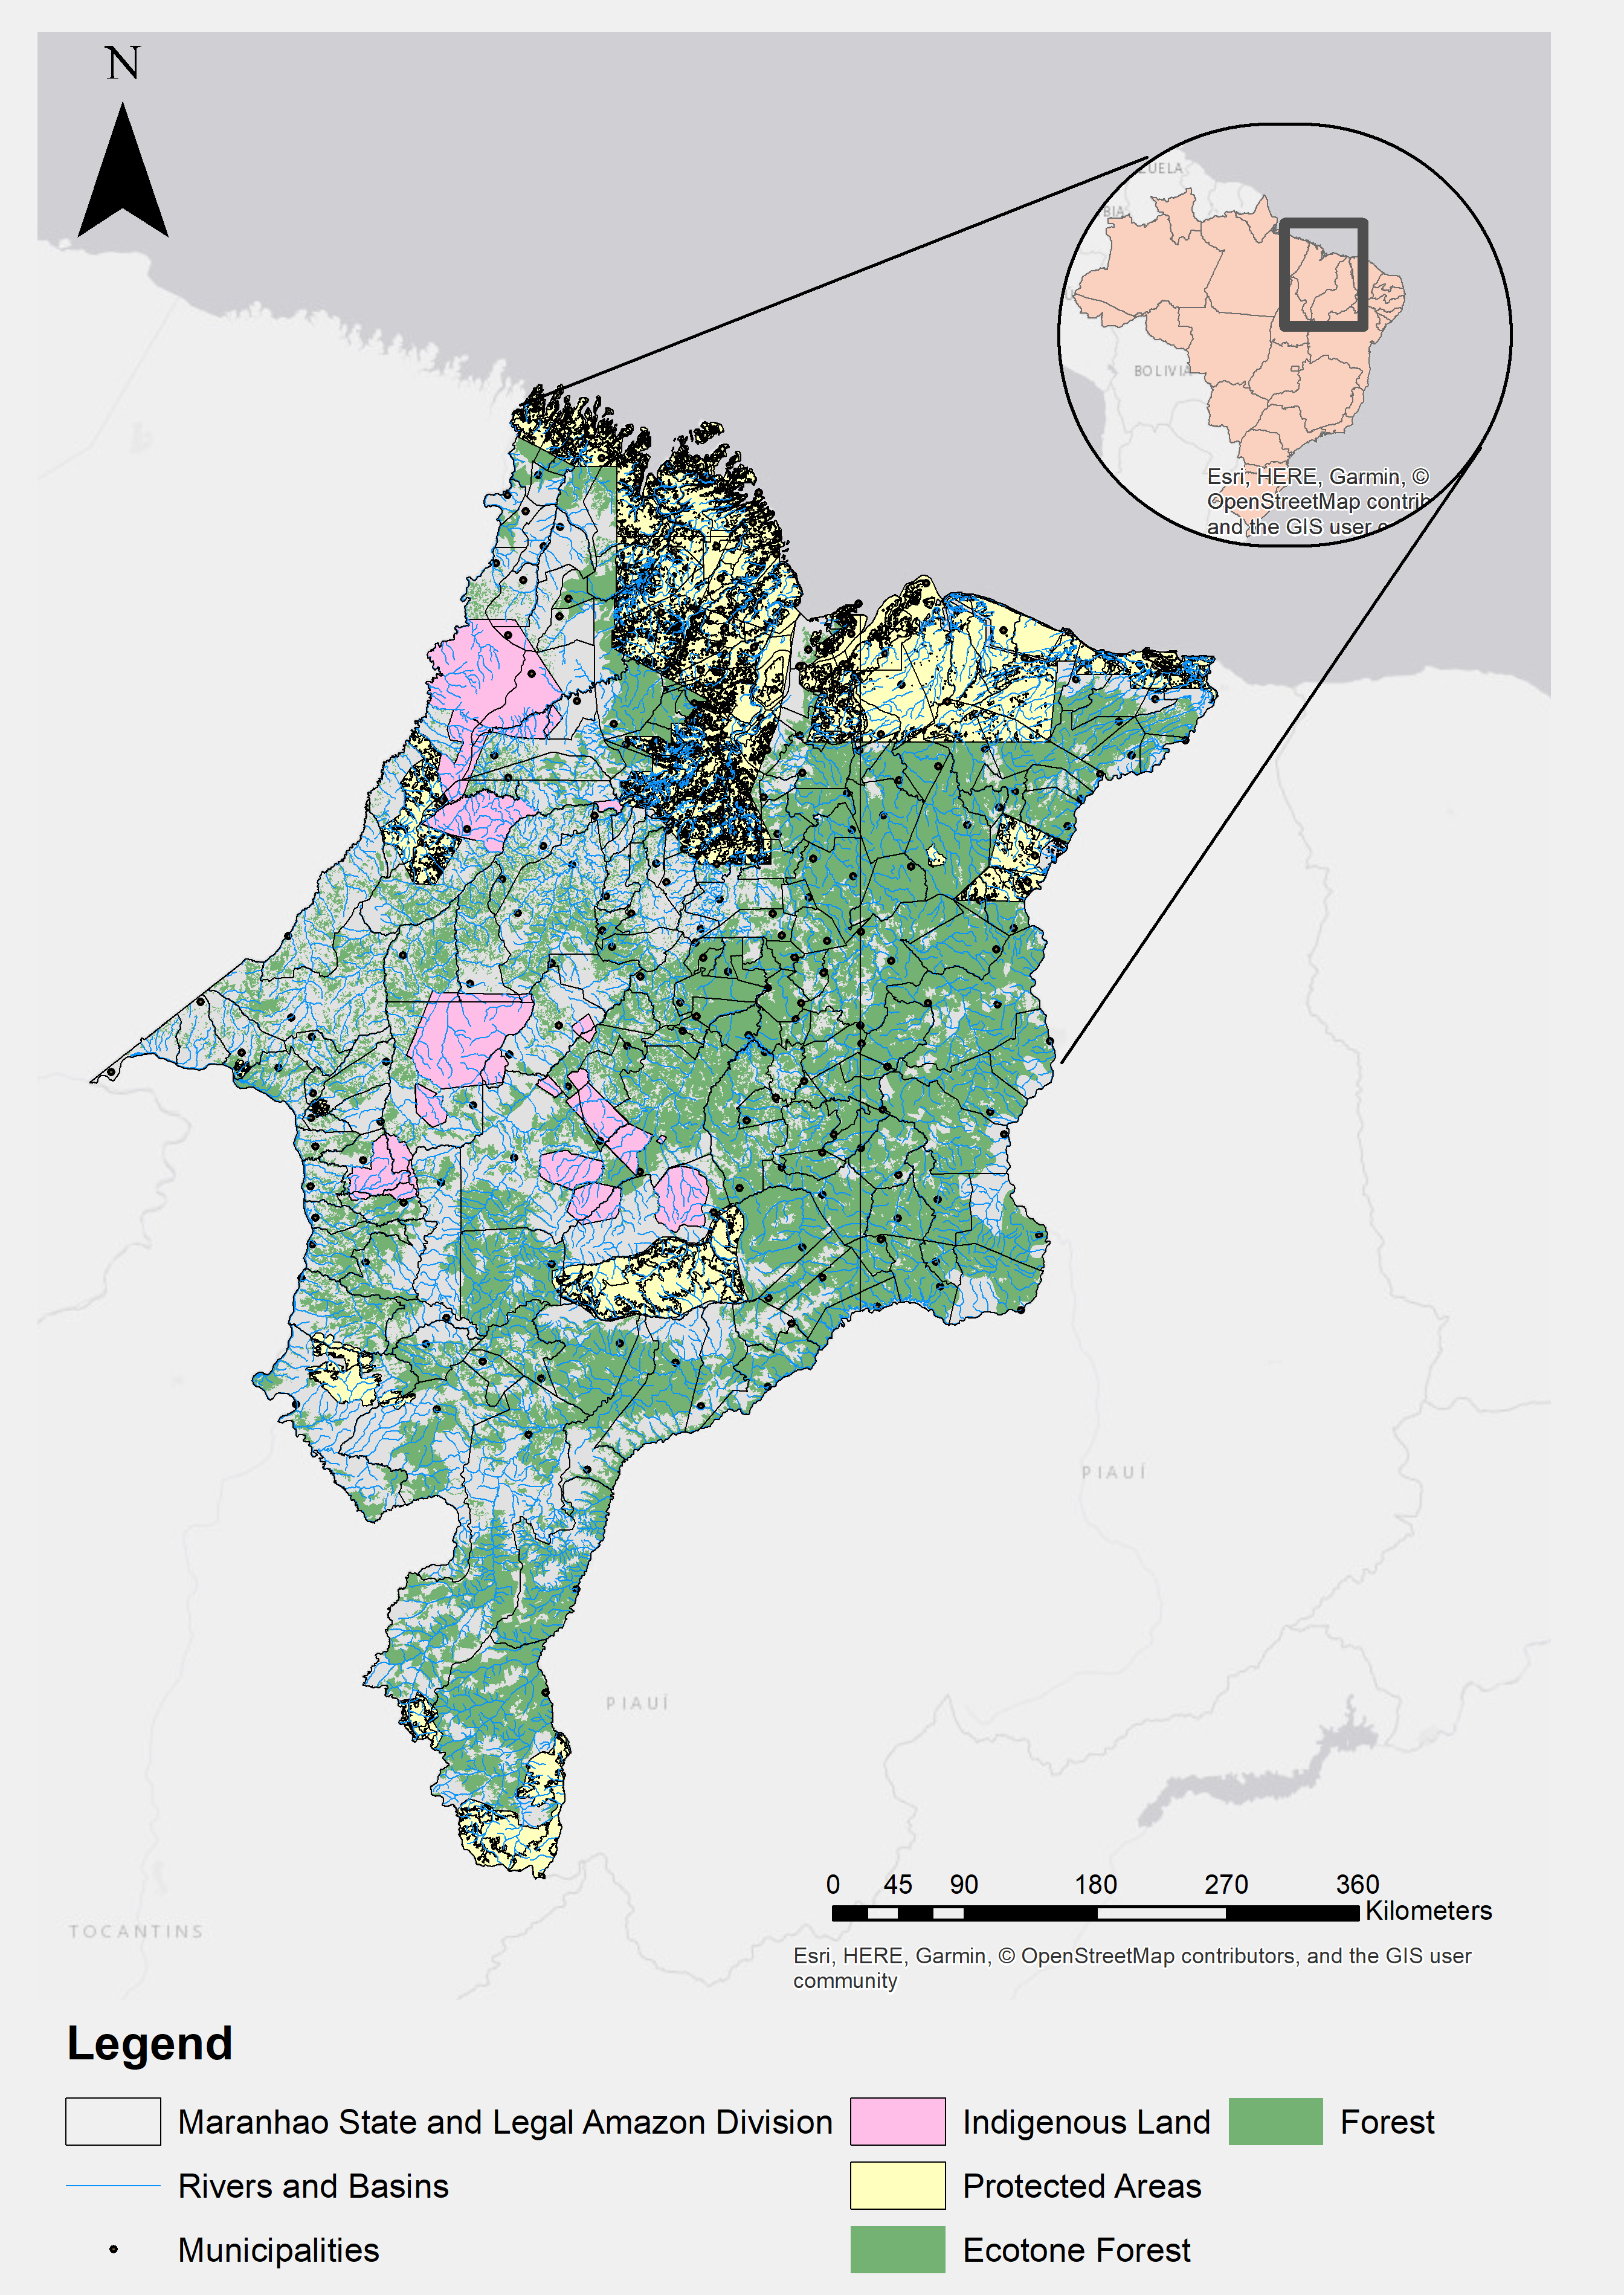
\includegraphics[width=1\textwidth, inner]{MaranhaoChapter2_Fig1.png}
\caption[Maranhão  state and the Legal Amazon delimitation]{Maranhão  State and the Legal Amazon delimitation. The map includes municipalities centre, rivers and basins, protected areas and indigenous land. Source: \citep{MMMAwebsite,nugeo_2018,embrapa_2018}.}
\label{fig:delimitacao2}
\end{figure}

%COLOCAR QUE EXISTE UM EMBATE PARA O TIPO DE VEGETACAO SECUNDARIA NO MARANHAO - SE EH ALGO ANTROPICO OU NATURAL POR PARTE DA REGIAO. VER O ARTIGO DE SOARES-FILHO 2013.


%Com base nos relatos de antigos viajantes de que regiões constituintes da Zona dos Cocais, como é atualmente denominado o ecótono presente em parte do território dos estados do Piauí e do Maranhão, continham várias populações de palmeiras, mas, especialmente em território maranhense, prevalecia uma floresta com características da pré-Amazônia e considerando os diferentes trabalhos e ensaios com várias espécies de palmeiras e suas respectivas propriedades no processo de recrutamento e sucessão ecológica, pode-se supor que a maciça concentração de grandes populações encontradas na região atualmente, seja reflexo de um intensivo processo de degradação das florestas originais com diferentes finalidades, partindo-se desde a exploração de territórios para pasto e agricultura, quanto ao extrativismo de plantas típicas das florestas presentes na região. O resultado desta degradação deixa evidente que, dentre estas espécies de palmeiras, o babaçu é uma das plantas mais expressivas e eficientes da comunidade pioneira.

\subsection{Deforestation in Maranhão}

%Studies of deforestation seem to vary from place to place. In Brazil, and specially Maranhão, deforestation happens depending on the status of development and welfare of the citizens in determining the extent of the forest loss. The requirement for income and economic growth results in growing demand for agricultural and forest derived products, like soy, timber and beef. The main causes of deforestation are assumed to be acting aggregated and the government finds these are the easiest and the most accessible ways of responding to their increasing economic pressures \citep{GEIST,CULAS11,CELENTANO_2017}.

%EXPLICAR A RAZAO PELA QUAL TEM DESMATAMENTO NO MARANHAO
Large-scale deforestation in the Maranhão Amazon forest began in the 1960s, when the military government promoted the occupation of this territory through the construction of highways and provided incentives for large farming projects on public lands and logging centres. In the 1980s, with the implantation of the iron mining project in the in the neighbouring state of Pará (Carajas Project), a railroad linking the mine to the port in Maranhão was built. Moreover, many pig iron facilities were installed in the Maranhão Amazon region, demanding large quantities of charcoal, which increased the pressure on forest resources \citep{CELENTANO_2017}.

%Colocar graficos 
%COMO EH ESSE DESMATAMENTO COMPARADO COM A AMAZONIA LEGAL E COM O RESTANTE DO CERRADO

While many existing studies have focused on the Amazon tropical forests \citep{PFAFF,PFAFF2,HAMMIG,GEIST, GEIST2, LAMBIN2,PFAFF3,ZAMBRANO,KUIK,COE,SOLER,NEPSTAD,ARIMA,PATZ,RICHARDS,RICHARDS2,CELENTANO_2017} due to the fact the ample environmental information was available through specific environmental policies, such as DETER, studying the Cerrado biome and, consequently, transition forests remains precarious. The first obstacle in monitoring the Cerrado biome is due to the high heterogeneity of the forests (open and dense forest, for example) which are substantially influenced by the climatic seasonality \citep{bayma_sano_2015}. The second challenge is related to the fact that there is no environmental policy in place to prevent rampant deforestation.  Nevertheless, in the context of the Amazon region, it is arguably crucial to understand the dynamic of Cerrado and its potential to influence adjacent forests of Amazonia since it provides a valuable endpoint from which climate and anthropogenic related aspects in the Amazon forest my be better understood (see Figure \ref{fig:defAmazonMA}).  

%In this sense, the Cerrado is the Brazilian biome most affected by human occupation in the last three decades, mainly due to the increasing pressure for the opening of new areas for the production of meat, grains and ethanol, which puts the survival of many species and the integrity of their habitat in risk \citep{mma_2018, bayma_sano_2015}. 


%Considered a transitioning state between semiarid and tropical environment, Maranhão's Cerrado figures the third position when comparing the amount of forest cleared in absolute values demonstrating that the end-point of Amazon forest is at risk (Figure \ref{fig:defAmazonMA}).  

\begin{figure}[H]
  \centering
  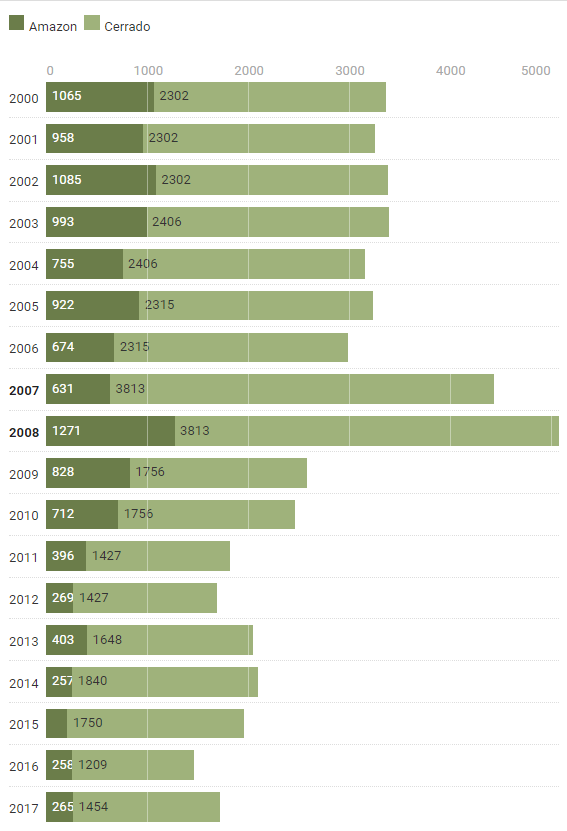
\includegraphics[width=1\textwidth, inner]{Chapter2/ChartMA_deforestation_chapter2.png}
\caption[Estimated Deforestation in Maranhão 2000-2017]{Estimated Deforestation in Maranhão 2000-2017 (sq Km). Source: \citep{MMMAwebsite}.}
\label{fig:defAmazonMA}
\end{figure}

%SERIA BOM COLOCAR O TREND DE DESMATAMENTO DE HANSEN PARA A PARTE QUE NAO TEM DADOS DO PRODES.

In the past many aspects have arguably contributed significantly to deforestation in the Cerrado Maranhão, such as the agricultural occupation of the Cerrado biome and the unconstrained use of mechanisation, propitiated by the predominantly flat relief of the region and the existence of good depth soil conditions and good water supply, making it possible to practice rainfed agriculture \citep{bayma_sano_2015}. In contrast, more recent forest losses  have been due to settlement projects, illegal logging, pasture, subsistence agriculture and commodities \citep{CELENTANO_2017, costa_2018}, and these drivers are deeply connected to the process of the state's development. More precisely, during the 40's, almost 85\% of the population was living in rural areas with low rate of population density (3,81). At that time, Maranhão had more than 200.000 km$^{2}$ uninhabitated, which included transition forest, Cerrado, and pre-Amazon forest. This "territorial gap" (/textit{fundos territoriais} in Portuguese) favoured the creation of several settlement projects along with the creation of federal roads and the Carajas railway project \citep{ferreira_2008}. Moreover, the increasing global demand for commodities affected the economic region significantly. For instance, fiscal incentives increased the production of soy, where the planted area increased from 42,6 km$^{2}$  in 1983/84 to 3,940 km$^{2}$ in 2004/05. The subsequent ecological tension zone coincides with the Brazilian agricultural frontiers, known as the deforestation arc, and is an area of intense exploitation. \footnote{The expansion of soybean cultivation in Brazil has shifted the
agricultural frontier to an area  known as MAPITOBA. This area includes the states of MAranhão,PIauí, TOcantins, and BAhia,, and has maintained its expansion across the Cerrado This led to deforestation and degradation, conservation conflicts and conflicts over land, increased burning, and displacement of traditional populations \citep{mustin__2017}}

%Despite the rich diversity in the three explained biomes, Maranhão is the state of the Legal Amazon that presents the lowest degree of occupation of the area with protected areas. The number of endangered, rare and endemic species in the most varied groups of animals and plants attest to the biological importance of the region, not only for the State of Maranhão, but for the country as a whole \citep{MARTINS_2011}. Only during the 2000s Maranhão invested an effort on environmental policies through the creation of conservational units, indigenous land titling and environmental policies in which helped to decelerate the deforestation path in the Amazon Maranhão.

%\subsubsection{The trend of deforestation in Maranhão}

As can be seen from the graph \ref{fig:defAmazonMA}, deforestation in the Amazon biome of Maranhão has decreased over the years. Great part of this reduction is likely due to protectionist policy enforcement in the region. In this regard, the national environmental policy established in 2004 involved the creation of the Action Plan for the Prevention and Control of Deforestation in the Legal Amazon (PPCDAm in Portuguese). In order to control land use and prevent further deforestation, the PPCDAm  also included the satellite-based monitoring programme called DETER, which alerts in real time the environmental police of illegal logging and deforestation. Importantly, until July 2018 there was no systematic satellite monitoring program for the other parts of Maranhão, such as the transitional forest of Cerrado and \textit{Caatinga}. But, in August of the same year, the National Institute of Spatial Research (INPE in Portuguese) together with several other institutions published an annual dataset covering 18 years of Cerrado biome deforestation and with this data it was possible to show the trends of deforestation in the Cerrado biome of Maranhão. As shown in Figure \ref{fig:defAmazonMA}, deforestation in great Cerrado, which includes the transitional forest, has been two times higher than in the Amazon region of Maranhão.

%Both areas, notwithstanding, show a decreasing trend according to official sources which imposes two questions questions to this study: 1- Is the decreasing deforestation trend in Amazon Maranhão during 2000 to 2017 displaced to the Cerrado Maranhão? Following the first question, 2- Is there a spillover effect from the environmental policy in the decreasing trend in deforestation on the Cerrado Maranhão? By applying an advanced technique and an alternative dataset and method, this study aims to be able to answer these questions.  

%Monthly data

%New technique applied to deforestation

\section{Material and Methods}
\subsection{Remote Sensing}  %mudar o titutlo

%Anthropic activities combined with natural events are significantly altering the Earth's land cover causing global climatic changes. When considering vegetation mapping for forest cover loss and forest regrowth path, traditional methods such as field surveys are time consuming, date lagged and generally too expensive. Over the past four decades, a feasible alternative considered by researchers and specialists is to apply remote sense technology and subsequent image analysis. 

The use of satellite time series along with statistical analysis can be helpful in understanding the characteristics of vegetation dynamics.  More precisely, since vegetation has a unique spectral feature (e.g., reflectance) it is possible to identify its unique characteristics from an optical remote sensor on a satellite. In such vegetation mapping, incorporating the spectral radiances in the red and near-infra-red regions into the spectral vegetation indices (VI) gives the possibility to estimate  forage  quantity  and quality  of  grass  prairie, for example \citep{xie_sha_yu_2008}. 
Earlier studies coarse spatial resolution data from the Advanced Very High Resolution Radiometer (AVHRR) was used to mainly monitor land cover changes at regional and global scales, however, since 2000, the availability of Moderate Resolution Imaging Spectroradiometer (MODIS) data with superior features relative to AVHRR has provided an improved basis for regional and global mapping \citep{huang_2014}.
%For instance, in 1999, a group of researchers around the world created the Global Land Cover 2000 (GLC2000) project extracting data from 1-km SPOT4-VEGETATION  imagery.\footnote{For the dataset, see http://www-gvm.jrc.it/glc2000/} After two years, US-NASA  released the  database  of  global  MODIS  land  cover  based  on  monthly composites from MODIS sensor for the period between January  and  December  2001 \citep{xie_sha_yu_2008}.\footnote{For the dataset, see http://duckwater.bu.edu/lc/mod12q1.htlm}

%In general, the  selection of  images  acquired  by  adequate sensors is largely determined by the mapping objective and accuracy, the cost of images, the climate conditions, such as a cloud-free image, and the technical issues that arise from interpretation and suitability.

%Images with low resolutions may be adopted only when the high level of vegetation classes are to be identified, while the images with relatively higher resolutions are used for fine-detailed classifications of vegetation. Also, from the mapping scale point of view, vegetation mapping at a small scale usually requires high-resolution images, while low-resolution images are used for a large-scale mapping. In the field of vegetation mapping, the most commonly applied sensors in decreasing spatial resolution order include NOAA–AVHRR, MODIS, Landsat (mainly TM and ETM+), SPOT, IKONOS  and QuickBird \citep{xie_sha_yu_2008}.\footnote{A detailed summary of satellites, sensors and databases relevant to vegetation can be found in \citet{horning_2010}.}




\subsubsection{MODIS}

%Falar do satelite MODIS e dos seus produtos

The MODIS sensor is flown on two spacecrafts. The Terra satellite is on an AM overpass, whereas the Aqua platform provides complementary observations in the afternoon. The instrument on-board NASA’s Terra satellite is a scanning radiometer system with 36 spectral bands, extending from the visible to the thermal infrared wave-lengths, and has a viewing swath width of 2330km by 10km. The Terra orbital configuration and MODIS viewing geometry produce full global coverage every one to two days, except for the equatorial zone where the repeat frequency is approximately 1.2 days \citep{zhan_2002, setiawan_2014}. The high temporal resolution of MODIS is a determining factor in phenological studies and spectral discrimination, and can be used to obtain detailed knowledge about the seasonal cycles of vegetation in biomes with strong seasonal contrast, such as the Cerrado biome and Ecotone forest. 

%The first seven bands are designed  primarily  for  remote  sensing  of  the  land  surface with  spatial  resolutions  of  250m  (Bands 1-2), 500m (Bands 3-7), and 1000m (Bands 8-36). Note that while the bands are commonly referred to as 250m and 500m, the actual resolution of the grids is 236 and 472m at the equator. 


%In addition, MODIS data is in a ready-to-use, atmospheric corrected, cloudless, and geo-referenced format.

Of the many data products derived from MODIS observations, we use two extensively used here: MCD12Q1 and MOD13Q1. The MODIS Land Cover Type Product (MCD12Q1) provides 13 science data sets (SDSs) that map global land cover at 500m spatial resolution at annual time steps for six different land cover legends from 2001-2016. In contrast, the MCD12Q1 product is created using supervised classification of MODIS reflectance data and includes 5 legacy classification schemes such as the University of Maryland classification (UMD), which recognises 17 classes, covering natural vegetation (11 classes), mosaic lands (2 classes), and non-vegetated lands (4 classes). A complete list of the classes and their definitions is given in Table \ref{UMD2} \citep{setiawan_2014, friedl_2018}.

%COLOCAR A TABLE 4 DO USER GUIDE MCD12Q1

The MODIS Vegetation Indices (VI) (MOD13Q1) product consists of time series comparisons of global vegetation conditions that can be used to monitor the Earth's terrestrial change detection. The two vegetation indices thatr we derive from these are the Normalized Difference Vegetation Index (NDVI) and the Enhanced Vegetation Index (EVI). The NDVI is a normalized transformation of the NIR (Near Infrared) to the red reflectance ratio standardized to range from -1 to 1.  \citet{ratana_huete_ferreira_2005} notes that this index is sufficiently stable to permit meaningful comparisons of seasonal, inter-annual, and long-term variations of vegetation structure, phenology, and biophysical parameters:

%Gridded vegetation index maps depicting spatial and temporal variations in vegetation activity are derived at 16-day and monthly intervals in support of accurate seasonal and inter-annual monitoring of the Earth’s terrestrial vegetation \citep{didan_munoz_2015}.

%COLOCAR AQUI A EQUACAO DO NDVI
\begin{center}
\begin{equation}
NDVI = \frac{\rho_{NIR} - \rho_{red}}{\rho_{NIR} + \rho_{red}} \label{eq:1.2} 
\end{equation}
\end{center}

where $\rho_{red}$ and $\rho_{NIR}$ are the surface bidirectional reflectance factors for MODIS bands 1 (620-670nm) and 2 (841-876nm). 

To optimise the vegetation signal and minimise atmospheric effect and soil background noise, the EVI index has been reported to be more responsive to canopy structural variations including canopy type. The EVI formula is written as:

%COLOCAR AQUI A EQUACAO DO EVI
\begin{center}
\begin{equation}
EVI = \frac{\rho_{NIR} - \rho_{red}}{\rho_{NIR} + C_{1\rho_{red}} - C_{2\rho_{blue}} + L} (G) \label{eq:2.2} 
\end{equation}
\end{center}

where $\rho_{red}$ and $\rho_{NIR}$ and $\rho_{blue}$ are the reflectance in MODIS bands 1,2 and 3 (459-479nm) and, C$_{1}$ and C$_{2}$ are the atmospheric resistance coefficients. L and G are the canopy background adjustment and the gain factor, respectively. The coefficients adopted for the MODIS EVI algorithm are, L=1, C$_{1}$ =6, C$_{2}$ =7.5 and G=2.5. The Enhanced Vegetation Index differs from NDVI by attempting to correct for atmospheric and background effects. In addition, EVI is superior in discriminating subtle differences in areas of high vegetation density than NDVI because the latter tends to saturate \citep{didan_munoz_2015, ratana_huete_ferreira_2005}.



%%%%%%%%%%%%%%%%%%%%%%%%%%%%%%%%%%%%%%%%%%%%%%%%%%%%%%%%%%%%%%%%%%%%%%%%
%%%%%%%%%%%%%%%%%%%%%%%%%%%%%%%%%%%%%%%%%%%%%%%%%%%%%%%%%%%%%%%%%%%%%%%%
%%%%%%%%%%%%%%%%%%%%%%%%%%%%%%%%%%%%%%%%%%%%%%%%%%%%%%%%%%%%%%%%%%%%%%%%
%Dar exemplos de pesquisas na area de desmatamento com MODIS VI products, explicar que sao bons indices para analisar o cerrado, dando embasamento. Ver RATANA (Ferreira e Huete, 2004). e BAYMAN VER NO CADERNO VERMELHO NOTAS BIBLIOGRAFICAS!!!! FALA DE DIVERSOS PAPERS COM USO DE MODIS!!!!
%%%%%%%%%%%%%%%%%%%%%%%%%%%%%%%%%%%%%%%%%%%%%%%%%%%%%%%%%%%%%%%%%%%%%%%%
%%%%%%%%%%%%%%%%%%%%%%%%%%%%%%%%%%%%%%%%%%%%%%%%%%%%%%%%%%%%%%%%%%%%%%%%
%%%%%%%%%%%%%%%%%%%%%%%%%%%%%%%%%%%%%%%%%%%%%%%%%%%%%%%%%%%%%%%%%%%%%%%%


\subsection{Study area characterization} \label{studycarac} %mudar o titutlo

%Caracterizacao da area de estudo

We compare deforestation trends within the vincinity of both sides of artificial border of the Legal Amazon.  To this end we experiment with three bandwidths of 25km, 50km and 100km in both east and west direction from the line giving a total of 6 sampled areas. The buffer zone is characterised by intense presence of Ecotone Forest and covers the east region (MA, hereafter) and west centre region (LM, hereafter) of the Maranhão state. As can be seen in Figure \ref{fig:buffer} the study area comprises more than one third of the State which represents our 100km buffer to east and west of the territory.

\begin{figure}[H]
  \centering
  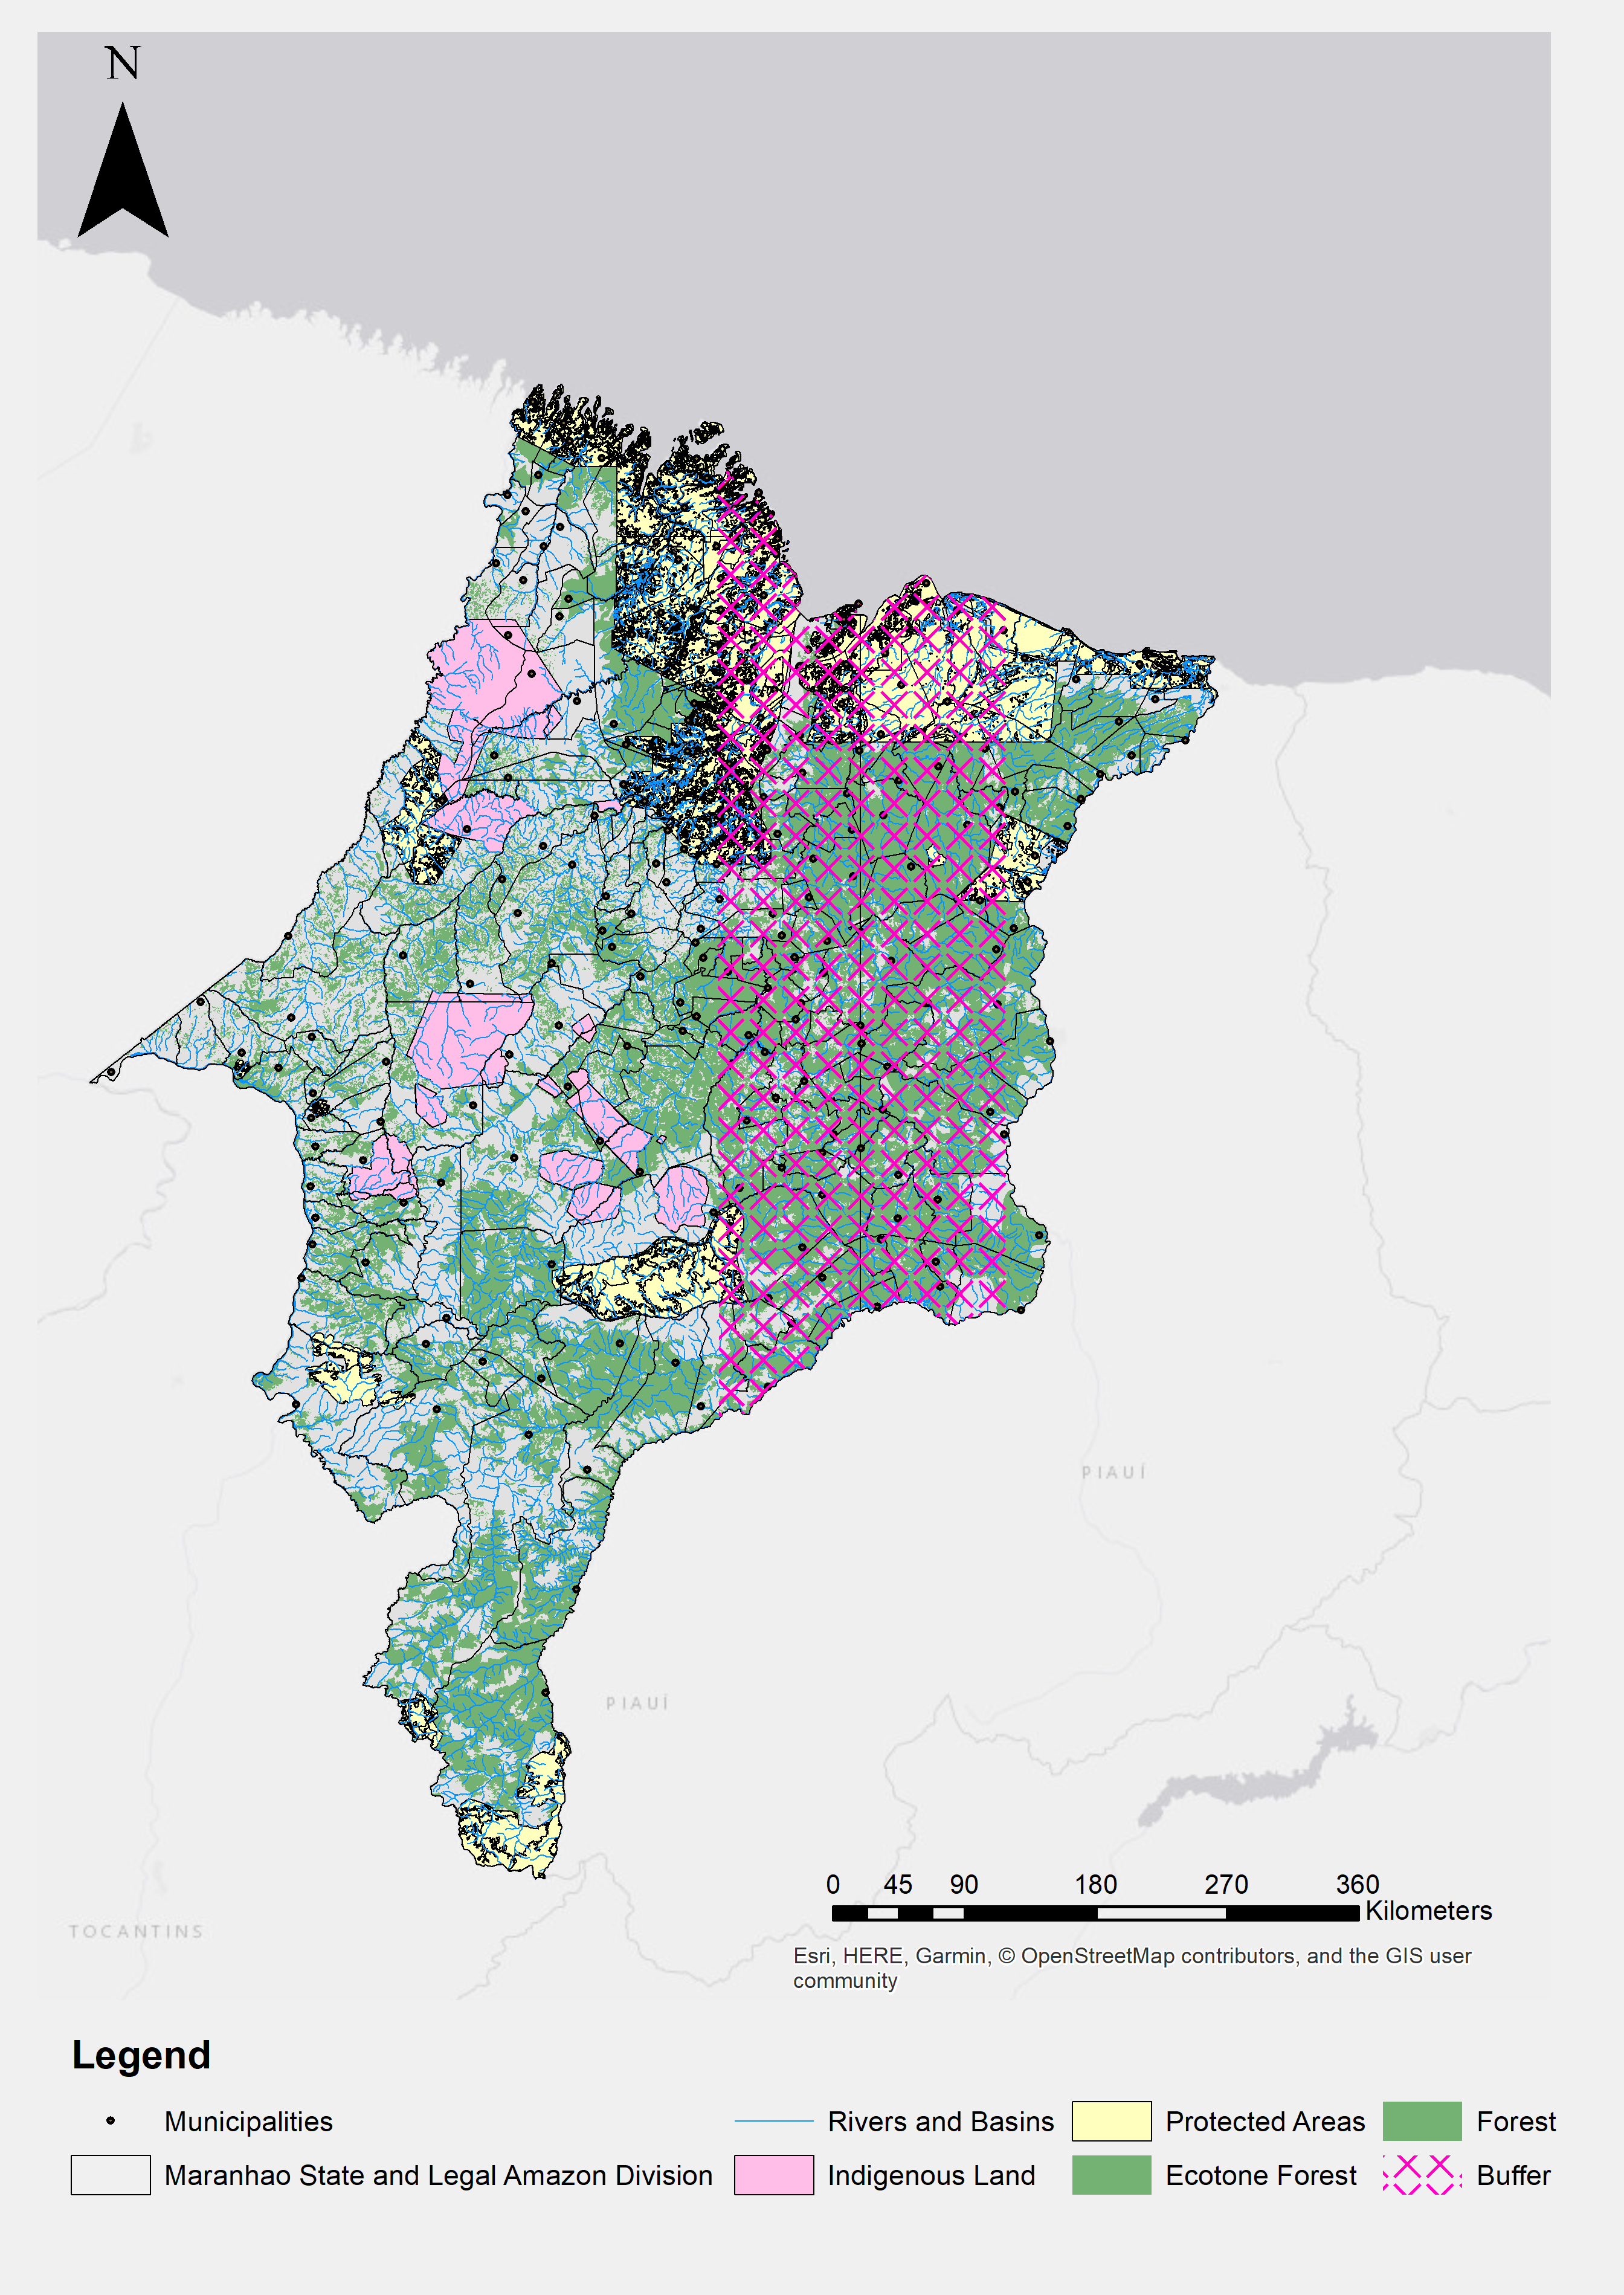
\includegraphics[width=1\textwidth, inner]{MaranhaoChapter2_Fig2.png}
\caption[Maranhão  state and 100km buffer departing from the Legal Amazon line to the east and west portion of the territory]{Maranhão  state and 100km buffer departing from the Legal Amazon line to the east and west portion of the territory. Source: \citep{MMMAwebsite,nugeo_2018,embrapa_2018}.}
\label{fig:buffer}
\end{figure}

%In climatic terms, the region presents large oscillation from north to south, predominating the tropical climate of the equatorial zone. In the LM region, the hot and humid tropical climate (As) predominates, typical of the Amazon region. The eastern region is marked by warm and tropical wet-dry or savanna climate (Aw). Temperatures are high, with annual averages higher than 25ºC, and towards the southeast of the studied region, it reaches 28ºC.

%CITAR GRAHBER_2015.

%outras variaveis ambientais: chuva, temp,

 %The dry period, which occurs from July to November, with a lower incidence of rain around the month of August, registers averages of the order of 17.1mm. The average annual precipitation varies from 1,500 mm in the western portion (LM), reaching 1,800 mm near the coast, while in the MA area precipitation is lower with 1,700 mm peaks in the plateaus. There are even smaller records in the MA region, which can reach 1,000 mm. 

%  relevo

%The relief of Maranhão is characterised by low planing surfaces in the midst of extensive fluvial plains, much of it is enclosed by Paleozoic and Mesozoic rocks of the Parnaíba Sedimentary Basin. 

The Study area is characterised by the occurrence of a rainfall regime with two well defined seasons. The rainy season, which is concentrated from December to June, reaching the highest peaks of rain in the month of March. The sample region presents itself as a large sloping platform in the south-north direction, with a low dip to the Atlantic Ocean.  The relief is classified into two large units: plains, which are subdivided into smaller units, and plateaus. Plains are considered to be surfaces with dimensions of less than 200 meters. The plateaus are areas with heights above 200 meters, restricted to the south-central areas of the studied region \citep{feitosa_2006, bolfe_2013}. Information on the geology of the ecotonic region were extracted from the official map published in 2011 by the Brazilian Institute of Geography and Statistics (IBGE) on the scale 1: 1,400,000.


%Geologia 
%The Oxisols are predominant in Maranhão. They are consist of stable, highly weathered, tropical mineral soils with highly oxidized subsurface horizons. In spite of the low natural fertility, these soils present physical conditions favourable to the agricultural crop, mainly the mechanized, because they are deep soils, well drained and they normally occur in flat relief or gently mountainous.

% MATERIAL SOBRE EXPOSICAO SOLAR DO MARANHAO

Solar radiation on the terrestrial surface has direct implications for local meteorology, especially in the studies on climate variability, interfering in satellite image analysis \citep{cohen_2002, dasilva_2004, pereira_2017}. The study region here is privileged in its energetic potential, since it is located completely in the region bounded by the Tropics of Cancer and Capricorn, and close to the Equator, a condition that favors high rates of solar irradiation. The State of Maranhão presents an average annual global irradiation value of approximately 5.0 kWh / m2 \citep{pereira_2017}. In the ecological tension zone, i.e. studied area, the municipalities of Caxias (5.4 kWh / m2) (MA), Chapadinha (5.3 kWh / m2) (MA), Bacabal (4.9 kWh / m2)(LM) and São Luís (4.9 kWh / m2) (LM) are distinct for having the highest solar irradiation rates. 

%COLOCAR MAPA IGUAL AO DE GRAHBER_2015 LOGO APOS OS FATORES CLIMATICOS

%Aspectos vegetacionais: quais classificacoes vegetacionais? 

%Also in this region, the transitioning vegetation is characterised by the contact of Savana / ombrophilous forest (SO), Savana / Seasonal Forest (SN), and Savana / Seasonal Savana besides the presence of secondary vegetation within the domain \citep{bolfe_2013}.

%outras variaveis ambientais: hidrologia e hidrovia


\subsection{Data preparation}  %mudar o titutlo

%Paragrafo com softwares usados, packages e livros guiados

Handling and preparing spatial data requires specific softwares. I used ArcMap 10.4.1, ArcPy 10.4.1, and the extensions Geostatistical Analyst, Spatial Analyst and Spatial Statistics from ArcToolbox \citep{esri_2016,arcpy_2016}, and MATLAB R2017a and its Statistics and Machine Learning and Image Processing Toolbox \citep{matlab_2017}. For statistical analysis and modelling I worked with R \citep{R_2018} and several packages specially 'MASS'\citep{MASS_2002}, 'mgcv' \citep{Wood_2003, Wood_2004, Wood_2011, Wood_2017} and 'gratia' \citep{Gavin_2018}.

\subsubsection{Vegetation Indices} %PRECISO COLOCAR MAPA COM A LOCALIZACAO DA REGIAO DE ESTUDO TIPO AQUELE TILE DO MUNDO!!!!!! 
Two remotely sensed datasets were used – Vegetation Indices 16-Day L3 Global 250m MODIS13Q1 and Land Cover Type Yearly L3 Global 500m MODIS12Q1. These products were retrieved from the online Application for Extracting and Exploring Analysis Ready Samples (AppEEARS) tool courtesy of the NASA EOSDIS Land Processes Distributed Active Archive Center (LP DAAC), USGS/Earth Resources Observation and Science (EROS) Center, Sioux Falls, South Dakota, \citep{didan_2015,didan_munoz_2015,sulla_2015,sulla2_2018}.

In the AppEEARS tool it is possible to define the region of interest by uploading a polygon file in shapefile format and the output file format is in Georeferenced Tagged Image File Format (GeoTIFF). When selecting GeoTIFF, one GeoTIFF will be created for each feature in the input polygon file for each layer by observation. After defining the area of interest, the tool uploads the input polygon and reproject the input file to the source projection for each data product using the Geospatial Data Abstraction Library (GDAL) (‘gdalwarp’ function and the PROJ.4 definition) for each data collection \citep{usgs_2018}. In this manner the MODIS images from MODQ131 and MCD12Q1 products were acquired in GeoTIFF format and the projection chosen was the geographic datum WGS84 – EPSG:4326. Two shapefile with the same coordinate system were used to extract the location LM and MA. LM (Legal Maranhão) refers to the area under the surveillance program to the west of the Legal Amazon line and, the MA (Cerrado Maranhão) refers to the area comprising the east portion of the buffer zone (see Figure \ref{fig:buffer}).

Next, a bounding box for each feature in the MODIS file was determined using the minimum and maximum latitude and longitude values, with a one pixel buffer applied to each corner. For each feature, the tool determines which spatial tiles intersect with the bounding box, and the tiles are then extracted from OPeNDAP \citep{ cornillon_2003} and mosaiced into a single image. The process is repeated and the MODIS images are ultimately configured into a time series image stack for each feature in the file. Reprojection is performed using nearest neighbour resampling technique and the latitude and longitude of the sample region are maintained in the conversion. Nearest neighbour resampling was selected to ensure that categorical data sets including quality data layers are able to be transformed \citep{usgs_2018}. 

A total of 776 images of the Vegetation Indices product MOD13Q1 were downloaded, from February 2000 to December 2016, and 16 images of the product Land Cover MCD12Q1 for the years 2001 to 2016. Also from the product bands MOD13Q1 the composite band day of the year was obtained, which provides the date (day of the year: 1 to 366) of acquisition of each pixel that composes the image; the band pixel reliability summary quality assurance - QA, which provides a summary of the quality of the pixels; and VI Quality detailed - QA band, which provides detailed pixel quality information. The product bands MCD12Q1 was downloaded the Land Cover type quality check – QC along with five different types of land cover data set.

\subsubsection{Climatic variables} %PRECISO COLOCAR UMA TABELA COM A LOCALIZACAO LAT LONG DA ESTACAO , O NUMERO DA ESTACAO, ALTITUDE E SITUACAO  
%Paragrafo com explicacao da aquisicao dos dados INPE colocando de onde peguei e citando as fontes de cada dado pego


The climatic data were obtained from the Meteorological Database for Teaching and Research of the National Meteorological Institute (BDMEP – INMET in Portuguese), which stores historical series of several conventional meteorological stations of the INMET station network. The access is through registration but is freely available for academic purposes \citep{bdmep_2018}. Each conventional weather station (see Table \ref{estacoesconvecionais} for the 9 stations in the sample area is composed of several isolated sensors that continuously record the meteorological parameters (e.g., temperature, precipitation, humidity, and solar radiation), which are annotated by an observer that sends the measurements to a collection center. In the historical series the maximum temperature is taken at 00 Universal Time Coordinated (UTC) of the day and the minimum temperature is collected at 12 UTC of the day. Precipitation is calculated by accumulating the last 24 hours collected at 12 UTC and solar radiation equals the number of hours the sun shines directly onto the surface as long as it is not blocked by clouds or any other obstacles. The relative humidity is obtained by the readings of the wet bulb temperature and dry bulb temperature at 12.00, 18.00, and 24.00 UTC \citep{vianello_2011}. We use the monthly average maximum temperature (MAMxT), monthly average compensated temperature (MACT), monthly average minimum temperature (MAMT), monthly average precipitation (MAP), monthly average relative humidity (MARH) and number of hours of sunlight in a month as total solar radiation (TS) from February 2000 to December 2016. 

\begin{table}[H]
\footnotesize
\caption{INMET Metereological Stations}
\begin{tabularx}{\linewidth}{H H H H H H}
\hline
\hline
Station Number (ID)  & Latitude & Longitude & Altitude & Name & \centering\arraybackslash Area\\
\hline
82571	&	-5.5	&	-45.23	&	153	&	BARRA DO CORDA 	& LM		\\
82970	&	-9.5	&	-46.2	&	285	&	ALTO PARNAIBA 	& LM		\\
82460	&	-4.21	&	-44.76	&	25	&	BACABAL 	& LM		\\
82765	&	-7.33	&	-47.46	&	193	&	CAROLINA 	&	LM	\\
82376	&	-3.26	&	-45.65	&	45	&	ZE DOCA  &	LM	\\
82476	&	-4.86	&	-43.35	&	104	&	CAXIAS 	&	MA	\\
82382	&	-3.73	&	-43.35	&	104	&	CHAPADINHA 	& MA	\\
82676	&	-6.03	&	-44.25	&	180	&	COLINAS  &	MA	\\
82280	&	-2.53	&	-44.21	&	51	&	SAO LUIS &	MA	\\
\hline
\hline
\multicolumn{6}{l}{\footnotesize  Note: Source: \cite{bdmep_2018,inmet_2018}.}
\end{tabularx}
\label{estacoesconvecionais}
\end{table}

\subsubsection{Cross Validation} 

Cross validation is a necessary approach when dealing with remote sensing data. MODIS Vegetative Cover Conversion (MOD44A) was acquired from the Global Land Cover Facility - University of Maryland \citep{glcf_2018} to conduct a validation process regarding the response variables (NDVI and EVI). The VCC product is used as an indicator of change and not as a means to measure change. It is available for vegetation burning and anthropogenic deforestation types of land cover conversion. In this sense, using this product as an indicator of accuracy is useful and reliable as states \citet{defries_2002}.

As part of the validation process, we used a finer resolution data set to check the accuracy of the algorithm applied to the MOD13Q product. \citet{Hansen_2013} provided results from time-series analysis of Landsat images in characterising the global forest extent and change from 2000 through 2017. The scenes utilised for the analysis contained forest losses during the period 2000–2016, defined as a stand-replacement disturbance, or a change from a forest to non-forest state. Encoded as either 0 (no loss) or else a value in the range 1–16, representing loss detected primarily for the years 2001–2016 \citep{gfc_2017}.\footnote{\begin{flushleft}Data Source: Hansen/UMD/Google/USGS/NASA. Data available on-line from: http://earthenginepartners.appspot.com/science-2013-global-forest. \end{flushleft}} Moreover, in 2018 Brazil's Spatial Research Institute (INPE), in accordance with the Brazil's Envinromental Ministry, published a data set covering the forest loss in the Cerrado Biome. This data consists of bi-annually images from 2000 to 2012 and yearly images from 2012 to 2016. Several sensors were used to create the composite data set, such as TM/Landsat5, ETM+/Landsat7, OLI/Landsat8, and LISS-III/IRS2. At a finer resolution, this product is a justified comparison between national and international land change products proving to be an acceptable validation procedure \citep{brito_2018}.


\subsection{Data Exploration and Interpretation}

After the selection of the variables there is a refinement process which configures the most important part of the research in order to achieve usable answers for statistical modelling. In this session, we will describes the steps taken to conduct the statistical analysis and the statistical method applied to the study.

\subsubsection{Response Variable}  %mudar o titutlo

% Paragrafo explicando como se deu a aquisicao dos pixels e tecnicas utilizadas interpretando por meio de figuras (colocar 2). 

In order to perform the analysis, NDVI and EVI images were imported onto MATLAB and scaled to the valid range of -0.2 to 1. Two images per month for each year were uploaded - excluding October and November during leap years because they had only one image within the month. The VI Quality detailed - QA band for each scene was converted to unsigned16bit according to the VI User Guide \citep{didan_munoz_2015} and it was used to create a Goodness mask to exclude pixels with clouds and not produced due to other reason than clouds. 

Before filtering the NDVI and EVI scenes with the VI mask, it was necessary to condition NDVI and EVI values to a specific threshold so to avoid values not related to forest. The criterion was taken following \citet{geerken_2009} and \citet{bayma_sano_2015} parameters to characterise forest in a transitional biome. Next, the VI indices are filtered and only values retained that have good quality according to the Goodness mask under the elimination of cloud coverage. 

With the Land Cover product MCD12Q1 it was required to resize and interpolate each image to the corresponding sizes of NDVI and EVI images. The interpolation method utilised followed a deterministic method called Nearest Neighbourhood (NN) or Thiessen method. The nearest method was considered because there is no extrapolation of the data, which would not have been suitable for categorical data and because it showed to be the fastest computation method with modest memory requirements \citep{ SLUITER_2009, matlab_2017}. After the interpolation, a land cover mask was produced to select only pixels in the images presenting forest classification. Following \citet{sulla2_2018}, the University of Maryland classification which corresponded to Land Cover Type 2 in the MCD12Q1 product was selected. The mask included different types of forests with at least 40\% of tree cover and canopy higher than 2m (see table \ref{UMD2} detailing each class definition). Forests presenting less than 40\% of tree cover were excluded because this does not characterise a transitioning forest being predominantly assigned to Cerrado biome only \citep{bayma_sano_2015}.  

\begin{table}[H]
\footnotesize
\caption{University of Maryland (UMD) legend and class definitions}
\begin{tabularx}{\textwidth}{l c X}
\hline
\hline
Name & Class & \centering\arraybackslash Description\\
\hline
Water	&	0	&	At least 60\% of area is covered by permanent water bodies	\\
Evergreen Needleleaf forest	&	1	&	Needleleaf Forests 1 Dominated by evergreen conifer trees (canopy >2m). Tree cover >60\%.	\\
Evergreen Broadleaf forest	&	2	&	Dominated by evergreen broadleaf and palmate trees (canopy >2m). Tree cover >60\%.	\\
Deciduous Needleleaf forest	&	3	&	Dominated by deciduous needleleaf (larch) trees (canopy >2m). Tree cover >60\%.	\\
Deciduous Broadleaf forest	&	4	&	Dominated by deciduous broadleaf trees (canopy >2m). Tree cover >60\%.	\\
Mixed forest	&	5	&	Dominated by neither deciduous nor evergreen (40-60\% of each) tree type (canopy >2m). Tree cover >60\%.	\\
Closed shrublands	&	6	&	Dominated by woody perennials (1-2m height) >60\% cover.	\\
Open shrublands	&	7	&	 Dominated by woody perennials (1-2m height) 10-60\% cover.	\\
Woody savannas	&	8	&	Tree cover 30-60\% (canopy >2m).	\\
Savannas	&	9	&	Tree cover 10-30\% (canopy >2m).	\\
Grasslands	&	10	&	 Dominated by herbaceous annuals (<2m).	\\
Permanent Wetlands	&	11	&	Permanently inundated lands with 30-60\% water cover and >10\% vegetated cover.	\\
Croplands	&	12	&	At least 60\% of area is cultivated cropland.	\\
Urban and built-up	&	13	&	At least 30\% impervious surface area including building materials, asphalt, and vehicles.	\\
Cropland/Natural Vegetation Mosaics	&	14	&	Mosaics of small-scale cultivation 40-60\% with natural tree, shrub, or herbaceous vegetation	\\
Non-Vegetated Land	&	15	&	At least 60\% of area is non-vegetated barren (sand, rock, soil) or permanent snow and ice with less than 10\% vegetation.	\\
Unclassified	&	255	&	 Has not received a map label because of missing inputs	\\
\hline
\hline
\multicolumn{3}{l}{\footnotesize  Note: Source: \cite{sulla2_2018}.}
\end{tabularx}
\label{UMD2}
\end{table}

Finally, to obtain a certain variation within each month, values of NDVI and EVI of the first period, with 15 first days of the month, were compared to the second period, with 30 days of the month. The assumption considered is explained in Table \ref{assumption2}. In this sense, the final scene/image would present pixels assuming the highest quality and no cloud coverage. At the end of the process, pixels were selected within the bandwidths of 100km, 50km, and 25km - measured departing from the artificial Legal Amazon line to the west and east portion of the State. When the pixel had a variation greater than 0.1 within a month, it was considered a disturbance.

\begin{table}[H]
\footnotesize
\caption{Algorithm Assumption for NDVI and EVI values}
\begin{tabularx}{\linewidth}{X X X}
\hline
\hline
$NDVI_{1} > NDVI_{2}$	& ->  $NDVI_{1} - NDVI_{2}$	 & Numbers (1) and (2) refer to the order of the period of the month \\
$NDVI_{1} <= NDVI_{2}$	& ->  $NDVI_{1} = NDVI_{2}$	 & Numbers (1) and (2) refer to the order of the period of the month. The second equation assumes that values did not change within the month and then the value assigned is from the last observation	\\
\hline
$EVI_{1} > EVI_{2}$	& ->  $EVI_{1} - EVI_{2}$	 & Numbers (1) and (2) refer to the order of the period of the month \\
$EVI_{1} <= EVI_{2}$	& ->  $EVI_{1} = EVI_{2}$	 & Numbers (1) and (2) refer to the order of the period of the month. The second equation assumes that values did not change within the month and then the value assigned is from the last observation 	\\
\hline
\hline
\end{tabularx}
\label{assumption2}
\end{table}


The approach above was undertaken for all the images corresponding to NDVI and EVI values for each month of each year, giving 406 final image results. For the leap year, the process stopped at the land cover mask filtering process. To compose a panel for each monthly period over 17 years, we took the sum of pixels signalled as disturbed for each of 406 images. 

\subsubsection{Covariates Variables} \label{covariate variables}  %mudar o titutlo

The climatic variables needed a more complex processing system since the data from weather stations were sparse. First, all the data was in a tabular format, i.e. all variables in one table, and geographic locations in the form of latitude and longitude coordinates and z-coordinates, such as elevation values, was created for each weather station using ArcMap. After localising the x,y,z coordinates, a shapefile for each station was created. Then the shapefiles were selected and extracted by year, using ArcPy environment. 

Next, an interpolation method was used to deal with areas with no data available. The method chosen was ordinary (point) Kriging which has been argued as the best interpolation technique available for sparse data \citep{SLUITER_2009}. Ordinary kriging is part of the probabilistic methods in which the concept of randomness is incorporated into the analysis. This method is the basic form of Kriging, where the prediction relies on a linear combination of the measured values and the spatial correlation between the data, determining the weights. As the mean is unknown we assume that intrinsic stationary exists in the data. This assumption may fail for our data set since this type of data are usually not stationary. To overcome this issue we used different sizes and shapes of neighbourhood to adjust the kringing ordinary model \citep{SLUITER_2009}. 

After the interpolation, the images were converted to raster, resampled to the size of the response variable, and exported to MATLAB environment. Generally, for temperature, precipitation, and other climate data, the best way to interpret and study these phenomenons is using anomaly measurements which corresponds to the difference between measurement and mean. In this sense, the average value of the variable of each image for each month and each year was computed, giving a total of 408 images analysed for both regions (MA and LM), and for each climatic variable, a total of 2,448 images. Following this procedure, the number of pixels with values higher and lower than the average value of the variable was extracted to a table. At the end, the table contained above and below values compared to the mean for each variable translating into 12 variables. A summary of the response and explanatory variables of this study is presented at Table \ref{tab:summarychapter2}.


\begin{table}[H]
\footnotesize
    \caption{Summary Statistics - Response and Covariate Variables}
      \begin{tabularx}{\linewidth}{X H H H H}
     \hline
     \hline
      Variable  & Mean & St. Dev. & Min. & \centering\arraybackslash Max.\\
     \hline
NDVI 25Km	&	626	&	731	&	0	&	4803	\\
NDVI 50Km	&	1279	&	1415	&	0	&	9185	\\
NDVI 100Km	&	2087	&	2175	&	0	&	12660	\\
EVI 25Km	&	8277	&	11353	&	0	&	73734	\\
EVI 50Km	&	2554	&	3861	&	0	&	25250	\\
EVI 100Km	&	8277	&	11353	&	0	&	73734	\\
Below Min Temp 25km	&	83711	&	57037	&	0	&	218320	\\
Below Min Temp 50km	&	159092	&	112926	&	0	&	436290	\\
Below Min Temp 100km	&	250820	&	171007	&	0	&	633370	\\
Above Max Temp 25km	&	105094	&	69290	&	0	&	218320	\\
Above Max Temp 50km	&	201308	&	134299	&	0	&	436300	\\
Above Max Temp 100km	&	287792	&	190863	&	0	&	633370	\\
Below Sunlight 25km	&	79678	&	47638	&	0	&	169150	\\
Below Sunlight 50km	&	167845	&	98578	&	0	&	434760	\\
Below Sunlight 100km	&	261061	&	149782	&	0	&	633370	\\
Below Humidity 25km	&	98957	&	50230	&	0	&	213400	\\
Below Humidity 50km	&	192560	&	97230	&	0	&	324620	\\
Below Humidity 100km	&	289185	&	140379	&	0	&	633370	\\
Above Precipitation 25km	&	90697	&	37384	&	0	&	191170	\\
Above Precipitation 50km	&	186745	&	77623	&	0	&	411370	\\
Above Precipitation 100km	&	292985	&	118665	&	0	&	633370	\\
    \hline
    \hline
    \multicolumn{5}{l}{\footnotesize  Note: Statistics refer to N=204 observations for 17 years (2000 - 2016). The below and above nomenclature}\\
    \multicolumn{5}{l}{\footnotesize refers to the mean of each variable.}
    \end{tabularx}
  \label{tab:summarychapter2}
\end{table}







\subsubsection{Modelling deforestation trends}  %mudar o titutlo

%Descrever modelos passados de desmatamento

Many recent studies of land cover changes focus explicitly on taking account of the trends and changes in the rates of environmental transformation in terms of their driving forces. More precisely, these studies try to identify the major causes of land-cover change within different geographical and historical contexts \citep{GEIST}. To this end proximate and underlying causes of deforestation models are concerned by the fact that some causes are direct in the sense that their occurrence or variation generates more or less deforestation through simple channels, while other causes are indirect in that they impact on the sources of deforestation through more complex channels \citep{MOTEL}. In this regard, the physical environment strongly influences where agents deforest, where many studies provide evidence that forests in drier, flatter, higher-fertility areas, with adequate drainage and thus more suitable for agriculture are more likely to be cleared \citep{ANGELSEN4}. In contrast, poor soil quality is also reported to lead to relatively high deforestation, since scant soil endowment fuels accelerated clearing for other activities, such as pasture \citep{GEIST,COSTA}. 

Environmental factors and  biophysical drivers are also increasingly being recognised as not only playing a role but being fundamental in deforestation \citep{GEIST}. To cite, \citet{BARNI} showed that, independent of the rate and magnitude of deforested areas, the areas affected by forest fires were dependent on the forest type and climate factors. Zones with ecotone influence tended to be deforested more than zones without ecotone influence, i.e., the more dense a forest is the less deforested will be. In addition, the largest occurrence of forest fires was observed in the zones with ecotone influence in years with \textit{El Nino} events, such as Maranhão state. The analysis also indicated that the areas most affected by forest fires during the studied period were associated with strong climatic events and the occurrence of these fires was amplified in the zones with ecotone influence \citep{BARNI}. These facts strongly suggest that it is pertinent to control for climatic aspects in ecotone zones when studying trends in deforestation.\footnote{In this study, ecological tension zone, ecotone zones and transitional forest have the same meaning. } 



%According to \citet*{MOTEL}, there are at least four models to study the impact of deforestation and its trends. 

%The first model included variables related to governance and institutional improvements as flatters for reduce the level of deforestation. The Environmental Kuznets Curve (EKC) model generally view better governance as an efficient means to achieve lower deforestation rates or environmental degradation while pursuing economic development. 

%Considering studies that describe the \textit{ex-ante} and \textit{ex-post} deforestation occurrence, the second model takes into account reforestation activities, which corresponds to the phenomenon occurring in many developed countries. Rather than considering overall deforestation, \citet*{MOTEL} explained that a model of Compensated Successful Efforts (CSE) would be appropriate to developing countries in order to fulfil the requirements established by the Reduced Emissions from Deforestation and Degradation mechanism. 



%In this context, many studies \citep{FENGER,DONG,LAMBIN1,FARGIONE,BARONA,ALDRICH,RICHARDS,KEENEY} concentrates in understanding causes of deforestation and land use changes to curb deforestation. In these studies, most commonly, a combination of proximate and underlying causes have been identified as the main drivers of deforestation.

\textbf{Statistical Modelling} 

%The most common approach used to model deforestation would be a linear model with a single or multiple terms. However, things are rarely this simple, and the model might interact in a complex way. The four approaches presented earlier consider the linear model as the first premise of the analysis but they are challenging when dealing with non-linear relationship found between variables \citep{griffin_2012}. In environmental analysis the data are seldom modelled adequately by linear regression models. 


%Introduzir o conceito de GAM 

For most ecological and climatic data sets at least some of the assumptions underlying a linear regression model are unlikely to be valid \citep{zuur_2011}.   To address this issue we here employ a generalized additive model (GAM). A literature review shows that GAMs are not extensively applied to deforestation models. \citet{COHEN_2008} showed that social factors appear to play a critical role that may ultimately determine disease risk when evaluated with environmental and climatic factors. They modelled incidence rates of a disease in Cuba as the response variable and deforestation as one of the exploratory variables. \citet{MENDES_2012} observed the relationship of deforestation, corruption and economic growth in the region of Legal Amazon, in Brazil and found no statistical evidence for the existence of a Kuznets curve. \citet{GREEN_2013} used a binomial GAM model to account for forest and habitat losses in protected areas on the Eastern Arc Mountains of Tanzania. More recently, \citet{BEBBER_2017} studied the impact of protected areas on global carbon emissions in America, Africa and Asia. They used splines regressions in GAMs and suggested that tropical PAs overall reduced deforestation carbon emissions by 4.88 Pg, or around 29\%, between 2000 and 2012. 


A GAM is a generalized linear model with a linear predictor involving a sum of smooth functions of covariates. Mathematically, GAM is an additive modelling technique where the impact of the predicted variables is captured through smooth functions \citep{larsen_2015}. In general, the model has a structure defined as: 

%\begin{center}
\begin{equation}  \label{eq:3.2} 
g(\mu_{i}) = A_{i} \theta + f_{1}(x_{1i}) + f_{2}(x_{2i}) + f_{3}(x_{3i},x_{4i}) + \dots
\end{equation}
%\end{center}

where $\mu{i} \equiv \displaystyle \E(Y_{i})$ and $Y_{i} \sim EF(\mu_{i},\phi)$. $Y_{i}$ is a response variable, $EF(\mu_{i},\phi)$ denotes an exponential family distribution with mean $\mu{i}$ and scale parameter, $\phi$, $ A_{i}$ is a row of the model matrix for any strictly parametric model components, $\theta$ is the corresponding parameter vector, the $f_{j}$ are smooth functions of the covariates, $x_{k}$, and ${i}$ refers to the unit of analysis \citep{Wood_2017}. This model allows for flexible specification of the dependence of the response on the covariates because the smooth functions are nonparametric. The smooth function $f_{j}$ is represented by basis expansions for each smooth, each with an associated penalty function controlling  smoothness. According to \citet{Wood_2004, Wood_2017}, the estimation can be carried out by penalised regression methods, and the appropriate degree of smoothness for $f_{j}$ can be estimated from data using cross validation or marginal likelihood maximisation.

The smooth function $f$ is composed of the sum of basis functions b and their corresponding regression coefficients $\beta$, written in the form of:

%\begin{center}
\begin{equation}  \label{eq:4.2} 
f(x) = \sum\limits_{j=1}^k b_{j}(x) \beta_{j}, \\
\end{equation}
%\end{center}

where k is the basis dimension (\citet{Wood_2017}, p.162). 

%In this way, it is possible to estimate $f$ in such a way that becomes a linear model. The smooth functions are also called splines or penalised splines. Splines are real functions that are defined by multiple sub-functions, where the polynomial pieces connect are called knots. The family of splines includes cubic splines, which fits a third-order polynomial on parts of the data and ensures that at the knots, the connections are smooth \citep{zuur_saveliev_ieno_2014}. It is important to observe that at the ends of the data, there will be discontinuity in the value taken by the spline. When the variable of interest behaves cyclically, it is necessary a correction procedure to these splines. The cyclic cubic spline is a potential solution to the problem because its basis has an additional constraint, which forces to no discontinuity at the end points of the spline \citep{Gavin_2018}.


%The choice of degree of model smoothness is essentially arbitrary and finding the optimal number of knots for a regression is obtained by finding the parameters $\beta$ and the smoothers that minimise the criteria in equation \ref{eq:5} \citep{zuur_saveliev_ieno_2014}.

%\begin{center}
%\begin{equation}  \label{eq:5} 
%\| Y - X\beta \|^{2} + \lambda \int_{}^{} f '' (x)^{2}dx\\
%\end{equation}
%\end{center}

%The second part of equation \ref{eq:5} is a penalty and contains $\lambda$ and an integral over the second-order derivatives, telling how smooth a curve is. A high value of $f''$ means that the smoother f is highly non-linear whereas a straight line has a second derivative equal to 0. In this case, if $\lambda$ is very large, the penalty for having a non-smooth curve is also large and if $\lambda$ is small, then there is a low penalty for non-smoothness \citep{zuur_saveliev_ieno_2014}. 

%In other words, when $f$ is very wiggly the penalty will take high values and when $f$ is ‘smooth’ the penalty will be low. If $f$ is a straight line then the penalty is actually zero. So the penalty has a null space of functions that are un-penalised: the straight lines in this case. Choosing the value of $\lambda$ requires further techniques. If $\lambda$ is too high or too low  then the data will be over-smoothed or under-smoothed, in both cases this will mean that the estimate $f$ will not be close to the true function $f$. Ideally, it would be good to choose $\lambda$ so that $f$ is as close as possible to $f$ \citep{Wood_2017}. A possible solution might be to choosing  $\lambda$ to minimise $\mathit{V_{o}}$ known as the ordinary cross validation using $\hat{f}$ estimation to fit all the data

%\begin{center}
%\begin{equation}  \label{eq:6} 
%\mathit{V_{o}} = \frac{1}{n} \sum_{i=1}^{n}\frac{(y - \hat{f_{i}})^{2}}{(1 - A_{ii})^{2}}\\
%\end{equation}
%\end{center}

%where \textbf{A} is the corresponding influence matrix, which is just the influence matrix for the model fitted to all the data. In practice, the $A_{ii}$ is replaced by their mean, resulting in the generalized cross validation score (GCV) \citep{Wood_2017}

%\begin{center}
%\begin{equation}  \label{eq:7} 
%\mathit{V_{g}} = \frac{n \sum_{i=1}^{n}(y_{i} - \hat{f_{i}})^{2}}{{[n - tr (\textbf{A})]^{2}}}\\
%\end{equation}
%\end{center}

%Interpretability 

%Flexibility and Automation

%Regularization

It is possible to regularise the smoothness of the predictor functions to prevent overfitting using the generalized cross validation score. Technically, GAM is an additive modelling technique where the impact of the predictive variables is captured through smooth functions, but provides a regularised, automatic and interpretable solution. Considering an additive model, the interpretation of the marginal effects of a single variable does not depend on the values of the other variables in the model. Also, predictor functions are automatically derived during model estimation \citep{larsen_2015}. 


%Dar exemplos de contribuicao desta metodologia para o desmatamento e em especial desmatamento na floresta tropical, amazonia e cerrado (floresta de transicao).



\textbf{Autocorrelation} %mudar o titutlo

In principle, when the nature of the data is time series, the timing of one period may depend on the timing of the previous year. This means that one should check for the possibility of autocorrelation and if necessary take into account of such the auto-correlation in the data. In GAMs it is possible to include an ARMA error structure. More precisely, the ARMA model has two parameters defining its order with the number of auto-regressive parameters (p) and the number of moving average parameters (q). Model \ref{eq:3.2} now can be expressed as


%\begin{center}
\begin{equation}  \label{eq:8.2} 
g(\mu_{i}) = A_{i} \theta + f_{1}(x_{1i}) + f_{2}(x_{2i}) + f_{3}(x_{3i},x_{4i}) + \dots + \varepsilon_{i}
\end{equation}
%\end{center}

where $\varepsilon_{i} = {\phi}\varepsilon_{i-1} + {\phi}\varepsilon_{i-p} + \eta_{i} $ is modelled as a function of the residuals of the p previous time points and white noise, and $\varepsilon_{i} = {\theta}\eta_{i-1} + {\theta}\eta_{i-q} + \eta_{i}$ is modelled as a function of the disturbance term and a past value of this disturbance term \citep{zuur_saveliev_ieno_2014}.

\textbf{Quantifying deforestation} 

The generalized additive model (GAM) with an exponential family distribution has been the most widely applied method to measure and quantify the non-linear association between phenology and covariates, such as meteorological conditions, mainly because it allows for non-parametric adjustments of non-linear confounding effects of seasonality and trends; \citep{alkemad_1998,BELL_2015,JOYE_2015,LUSK_2016,SADAT_2016,HALPERIN_2016, SANTOS_2017,TAPIA_2017,LIU_2018,MORENO_2018}.  In an attempt to quantify forest disturbance as proxy for deforestation, we apply a GAM with a negative binomial distribution and a logarithmic link function. The negative binomial distribution suitable for this study since the variance of deforestation is much larger than the mean, which is frequent feature of ecological data \citep{zuur_2011}. More precisely, the means of NDVI and EVI are to 0.04\% and 0.01\% of their variance, respectively. Hence, the response variable is negative binomial distributed. The full description is as follows:

\begin{flushleft}
 \hspace{4em} $Y_{is}$ $\sim$ NB($\mu{_i}$,k) 
\vspace{-0.2em}
\begin{equation}
\hspace{-12em}E(Y_{i}) = \mu_{i}, and \hspace{1em} var(Y_{i}) = \mu_{i} +\frac{\mu^{2}_{i}}{k} \label{eq:9.2}    
\vspace{-1em}
\end{equation}
 \hspace{4em} log($\mu_{i}$) = $\alpha$ + $f_{j}$($X_{i1})$ $+ \dots +$ $f_{j}(X_{iq})$ \hspace{1em} or  \hspace{1em} $\mu{i}$ = $e^{\alpha +f_{j}(X_{i1})+\dots+f_{j}(X_{iq})}$  \\    
\end{flushleft}

$Y_{i}$ is the response variable at observation i. The notation $f_{j}$($X_{i1}$) stands for 'smoothing function of the covariate variable X', and \textit{NB} is a negative binomial distribution with mean $\mu_{i}$ and dispersion parameter k. In general, negative binomial distributions are used to model overdispersed count data or Poisson data.  

The geometric distribution is a negative binomial with overdispersion parameter, k, set to 1. In this sense, the variance increases as a quadratic function of the mean \citep{zuur_saveliev_ieno_2014}. Correcting the data for overdispersion with the geometric distribution, the model is stated as

\begin{flushleft}
 \hspace{4em} $Def_{\scriptscriptstyle (NDVI_{i}, EVI_{i})} = \alpha + f_{\scriptscriptstyle Year}(Year) + f_{\scriptscriptstyle Precip}(aPrecipitation) + f_{\scriptscriptstyle Max Temp}(aMax Temperature)$ 
\vspace{-0.2em}
\begin{equation}
  + f_{\scriptscriptstyle Min Temp}(bMin Temperature) +  f_{\scriptscriptstyle Sunlight}(bSunlight) + f_{\scriptscriptstyle Humidity}(bHumidity) \label{eq:10.2}    
\vspace{-1em}
\end{equation}
\end{flushleft}

%Colocar o modelo de desmatamento escolhido explicar cada variavel do modelo, novamente. 

where $Def_{\scriptscriptstyle (NDVI_{i}, EVI_{i})}$ is the response variable that can assume NDVI and EVI values for three different bandwidths (25km, 50km, 100km) in each month \textit{i}, and $i=1,\dots,204.$ The remaining variables are the intercept $\alpha$ andthe additive smoothing functions of the explanatory variables Year,  and the covariates Precipitation, Humidity, Max and Min temperature and sunlight. \textit{a} and \textit{b} refers to the sum of pixels above and below the mean, respectively.

%Explicar processo de escolha do modelo de desmatamento (forwarding selection, Zuur). 

The model selection followed the forwarding approach of \citealp[p.391]{zuur_saveliev_ieno_2014}. The model started with a GAM that used one variable, then fitted 13 different models and a different set of smoothers (penalised splines "ps", cubic splines "cr", and cyclic splines "cc") and compared their Akaike information criterion (AIC). The model with the lowest AIC was elected as the main model and, then it was fitted to 12 different models, each with the addition of the variable with the lowest AIC. The forward selection stopped at the moment the main model had the best AIC value comparing to the remaining models. After the model selection, an autocorrelation test was conducted but none of the models appeared to be autocorrelated. The model, including the splines takes the form of:

\begin{flushleft}
 \hspace{1em} $Def_{\scriptscriptstyle (NDVI_{i}, EVI_{i})} = \alpha + f_{\scriptscriptstyle Year}(Year, bs= cc) + f_{\scriptscriptstyle Precip}(aPrecipitation, bs= cr) +$ 
%\vspace{-0.2em}
\begin{equation}
 f_{\scriptscriptstyle Max Temp}(aMax Temperature, bs= cr) + f_{\scriptscriptstyle Min Temp}(bMin Temperature, bs= cc) +  \label{eq:11.2}    
%\vspace{-1em}
\end{equation}
 \hspace{1em} $f_{\scriptscriptstyle Sunlight}(bSunlight, bs=cc) + f_{\scriptscriptstyle Humidity}(bHumidity, bs= ps)$
\end{flushleft}


Due to the fact that his method is relatively recent, it is important to acknowledge that the algorithms available for choosing the optimal smoothing parameter are  not  yet  well  developed  and  can  generate  misleading  results if care is not taken. Furthermore,  use  of  such  criteria  can  often  lead  to  over-fitting  and  deliver  implausible  associations.  The choice  of  smoothing  parameters  for  smoothing  splines  in  GAM  should  therefore  always  be  accompanied  by  a  graphical  verification  of  functional  associations  with  the outcome  to  verify  clinical  plausibility \citep{moore_2011}.

\subsubsection{Model Validation}  %mudar o titutlo

Validating the results from the algorithm applied to the MOD13Q1 and MCD12Q1 images required features of the machine learning domain. In summary, machine learning algorithms can figure out how to perform important tasks by generalizing from examples. This is often feasible and cost-effective where manual programming is not \citep{Domingos_2012}.

There are different types of machine learning algorithms, where the most mature and widely used one is classification. According to \citet{Domingos_2012}, a classifier is a system that inputs a vector of discrete and/or continuous feature values and outputs a single discrete value, the class. For this study, the filter classifies pixels into deforested or not deforested and its input may be a Boolean vector $x = (x_{1},\dots, x_{j},\dots, x_{d})$ where $x_{j} = 1$ if the \textit{j}th pixel is deforested and $x_{j} = 0$ otherwise. A learner inputs a training set $(x_{i}, y_{i})$, where $x_{i} = (x_{i,1},\dots, x_{i,d})$ is an observed input and $y_{i}$ is the corresponding output, and output is a classifier. The test of the learner is whether this classifier produces the correct output $y_{t}$ for future examples $x_{t}$. A feasible classification validation is the confusion matrix. 

%Explicar aqui o metodo usado para fazer a confusion matrix.

The confusion matrix is a two by two table that contains four outcomes produced by a binary classifier. The classification scheme divides the data randomly into a training set, a test set and a validation set. The training method is the Scaled Conjugate Gradient (SCG), which is a supervised learning algorithm for feed-forward neural networks \citep{mor_1993}. In order to optimise the performance, an iterative random sampling approach is applied. The Cross-Entropy approach is based on sampling and updating an underlying distribution function over the set of feasible solutions \citep{HU_2009}. Finally, calculations for the confusion matrix are done based on minimum excluded (MEX) calculations \citep{matlab_2017}.

The four outcomes produced by the confusion matrix are true positive, true negative, false positive, and false negative. The true positives (TP) refer to the number of positives divided by all the positive outcomes and the same applies to true negatives (TN). False positives (FP) indicate the number of pixels assigned as positive but are, in fact, negative, divided by all the positive outcome. In turn, false negatives (FN) follow the same interpretation as false positives. 


%Explicar os metodos de validacao para as variaveis Response


To validate the response variable results, it was used the MODIS Vegetative Cover Conversion (VCC) for the available period (2000-2005). The product is further divided in Deforestation product (MOD44A${\_}$C) and Burn product (MOD44A$\_$B) and both were used to compute the validation test. 

The method for the deforestation product is derived from the original space partitioning method \citep{zhan_2002} and relies on a decision tree classification algorithm \citep{breiman_1984} to determine antecedent vegetation condition and compares this to current vegetation condition. Change due to burning product is derived using the difference Normalized Burn Ratio (dNBR) methodology from two scenes a year apart, as proposed by \citet{key_2004}.  Tests were computed per season (raining season and dry season) and per vegetation index (NDVI and EVI). The confusion matrix showed 100\% true positives and true negatives, which gives high stability to the algorithm created and applied to the NDVI and EVI indices. 

%ROBUSTNESS CHECK AND VALIDATION WITH HANSEN AND PRODES

Checking the results with other datasets was an alternative approach taken in this study. A confusion matrix was applied to the \citet{Hansen_2013} and Brazilian (INPE) data sets \citep{brito_2018}. The results showed no difference from the results presented in the VCC validation method. The confusion matrices are provided in the Appendix \ref{appendix2}. 

%Explicar os metodos de validacao para as variaveis Explicativas 
The covariates variables were validated using cross-validation processes during the interpolation procedure. Cross-validation uses all the data to estimate the trend and autocorrelation models. It removes each data location one at a time and predicts the associated data value. This is also known as leaving-one-out, and can be computed for all or a subset of the data locations \citep{esri_2016}.

In the kriging method, the cross-validation produced other results that helped evaluate the best interpolation method. More specifically, the Average Standard Errors (ASE) and Root Mean Square Standardized Error (RMSE) were computed. If ASE from the model are close to the RMSE then the model is correctly assessing the variability in prediction. If ASE are greater than RMSE then the model is overestimating the variability of the prediction and, finally, if the ASE are less than RMSE, the model is underestimating the variability in predictions. For the covariates analyses, ASE were on average 95\% of the value of the RMSE, proving to be a reasonable interpolation method with valid results.

In terms of statistics, model validation with additive modelling was visual rather than numeric after the model selection phase. The steps taken included plotting the residuals against fitted values to identify violation of homogeneity, and plotting the residuals against each variable in the model and check for patterns. Also, a histogram of the residuals was examined to verify normality. 

%Criar um diagrama parecido com o de Griffin, p. 34 para descrever MODEL VALIDATION


\section{Results}  %mudar o titutlo

\subsection{Deforestation trend in a ecotone zone of Maranhão} \label{resultssection1.2}

%Explicar response over year

Our baseline model includes 204 monthly observations of NDVI and EVI values changing over the years with five influencing covariates (Precipitation, Max Temperature, Min Temperature, Sunlight and Humidity). The baseline model was applied to three different distance spans (25km, 50km, 100km) considering the Legal Amazon line.\footnote{It is important to acknowledge that the numerical results of the model should not be interpreted in the same manner as the linear regression results. According to \citet{Wood_2011} in \citet{zuur_saveliev_ieno_2014}, p-values close to 0.05 can be around half of their correct value when the null hypothesis is true. This means that smoothers with p-values smaller than 0.001 can be trusted but p-values of 0.02 to 0.05 need to be viewed with caution.} 

In general, the deviance explains the models close to the artificial line better. At large distances (100 km), most of the covariates do not have a significant effect, and thus will be omitted from this part of analysis. Table \ref{results1} gives the summary of the results including deviance, AIC, p-value, degrees of freedom, and the estimated value of the function. The best way to understand and interpret GAMs is through visual representation. Considering that the results produced several models, we define the name of these models according to the location status, whether in Cerrado Maranhão (MA) or Legal Maranhão (LM), the bandwidth or distance from the Legal Amazon line, in which are 25km,50km and, 100km, and, finally, regarding each response variable that in our case is related to NDVI (n) and EVI (e) values. We add an indicative variable to indicate raining (r) and dry (d) seasonality. Plotting the smoothing functions, it is possible to check for the path of deforestation through the years and the climatic state during that period. The blue line refers to positive changes in deforestation or increments, and the red line indicates negative changes in deforestation or decreases \citep{Gavin_2018}. 

\begin{sidewaystable}
\begin{table}[H]
\footnotesize
\caption[Models Output of GAMs]{Models Output of GAMs}
\begin{tabularx}{0.88\linewidth}{lxxxxxx}
\hline
\hline
Model  & AIC &   Deviance Explained &  AIC &   Deviance Explained & AIC &   Deviance Explained\\
\hline
Baseline Model & & & Raining Season &  &  Dry Season &    &\\
\hline
ma25n & 4592.974 & 15\% & 3008.928 & 53.8\%  & 3029.610 & 52.3\% \\
lm25n & 4753.342 & 30.9\% & 3082.583 & 44\% & 3330.420 & 54.6\% \\
ma25e & 5382.682 & 20.1\% & 3486.908 & 52.1\% & 3533.256 & 50.9\%\\
lm25e & 5450.606 & 36.4\% & 3369.937 & 63.1\% & 3812.126 & 65.6\%\\
ma50n & 5035.296 & 17.3\% & 3402.803 & 60\% & 3390.411 & 42.2\%\\
lm50n & 5010.875 & 24.5\% & 3241.013 & 55.8\% & 3498.748 & 35.1\%\\
ma50e & 6123.032 & 20.5\% & 4154.889 & 62.6\% & 4051.907 & 47\%\\
lm50e & 5921.597 & 29.3\% & 3886.190 & 63.2\%& 4112.314 & 48.5\%\\
ma100n & 5312.836 & 16.6\% & 3723.872 & 62.2\%& 3562.066 & 45.2\%\\
lm100n & 5318.571 & 30.5\% & 3552.311 & 52.7\% & 3701.532 & 47.2\%\\
ma100e & 6097.770 & 23.6\% & 4176.352 & 59.4\% & 4051.806 & 45.3\% \\
lm100e & 5901.040 & 33.4\% & 3906.004 & 59.5\% & 4097.055 & 46.7\% \\
\hline
\hline
\multicolumn{7}{l}{Note: Models Output of GAMs with Akaike’s Information Criteria (AIC) and Deviance goodness-of-fit statistic for each statistical model}
\end{tabularx}
\label{results1}
\end{table}
\end{sidewaystable}



With respect to the model \textit{ma25n}, the explained deviance is 15\%, the variance was set to 1 in the geometric negative binomial distribution. The explanatory variable year is significant at 1\% level, and the smoothers significant at 1\% level are \textit{Min Temperature}, \textit{Max Temperature}, \textit{Humidity} and \textit{Sunlight}. The degrees of freedom for the smoothers are 2.4, 6.8, 4 and 7.9. In summary, for MA at 25km, deforestation had a positive effect after 2010 and, through the years, deforestation decreased during periods of low humidity (high thermal oscillation). It is also deduced from the model that deforestation decreased during periods of more hours of sunlight. There were more deforested pixels in periods where temperature declined. 

For the model \textit{lm25n}, the explained deviance is 30.9\%, the explanatory variable year is significant at 5\% level, the smoothers significant at 1\% level are \textit{Max Temperature}, \textit{Humidity} and \textit{Sunlight}. The degrees of freedom for these smoothers are 8.6, 6.1 and 1.4. The results are similar to the \textit{ma25n} model by showing that deforestation also decreased during periods of less humidity and extreme higher levels of precipitation. Examining deforestation as a function of the year showed that there was a positive effect, i.e., increments on forest loss, during the beginning of the 2000's.

%Explicar o de \textit{ma25e} e o ml25e


Models with EVI values were considered better in terms of cross validation. Model \textit{ma25e} shows that deforestation increased over time with a positive peak after 2010. Deforestation also increased when the covariates sunlight and minimum temperature decreased. For maximum temperature, the negative effect is greater than the positive effect but, in essence, deforestation decreased with higher temperatures. On the Legal Maranhão side, the results of the model \textit{lm25e} show that all variables are significant at the 1\% level. The model explains 36\% of the changes in EVI values, i.e., deforestation. From 2007 to 2012, deforestation increased in the region. The positive effect happened during periods of higher temperature and low humidity. 


%explicar o de \textit{ma50n} e \textit{lm50n}
%Expanding the buffer zone to 50km, the model \textit{ma50n} shows the same pattern as 25km analysis with the difference that deforestation increased with higher levels of precipitation. The model explains 17.3\% of NDVI values for that region. Deforestation through the years had only a negative effect between 2002 and 2004 and the most of deforestation occurred when levels of sunlight were low. For the \textit{lm50n} model, it is also observed the same pattern with the exception that, at 50km band, deforestation declined with higher levels of temperature although the pattern for deforestation continued to decrease at extreme higher levels of precipitation. 

%explicar o de \textit{ma50e} e \textit{lm50e}

%Checking for EVI values, the model \textit{ma50e} still showed forest loss increment for the period after 2010, giving the same result as \textit{ma25e}. In turn, deforestation happened during low temperature period and with less hours of sun. It shows that at 50km, increased deforestation happened when precipitation level was higher than the average and deforestation and humidity had a negative linear relationship. This result differs from the \textit{lm50e} model, in this model, humidity and deforestation have a non-linear relationship and the latter occurred when the former was at low levels. Forest loss also happened when temperatures increased and, looking in function of the years, deforestation decreased after 2004 and increased back again after 2010. 


%explicar o \textit{ma100n} e \textit{lm100n} 

%For the last set of models with the largest bandwidth the deviance explained between 16\% to 33\% of deforestation in those areas. Starting by the model \textit{ma100n}, many of the covariates have lost significance. The explanatory variable year has no longer an effect on deforestation and higher levels of temperature have a linear negative relationship with deforestation. At the end, deforestation decreased during lower levels of humidity or, higher thermal oscillation. Model \textit{lm100n} showed that deforestation increased at higher levels of precipitation but when the levels of precipitation reached values higher than 75\% of the sample, deforestation decreased significantly. At 100km buffer, deforestation decreased during periods with less glaring sunlight.

%explicar o \textit{ma100e} e ml100e
%With the model \textit{ma100e}, deforestation increased during 2008 to 2012 with a slightly decrease in 2010. Deforestation varied considerable with the decay of humidity levels, this can also be mirrored with the temperature covariates, both seem to show that deforestation increased within their extreme values. Again, deforestation decreased with the increasing amount of precipitation during the studied period. Finally, the 100km band analysis for the Legal Maranhão area shows that all the variables are significant at 1\% level and, apart from the same results found in model \textit{lm100n}, deforestation decreased in a short period of 2007 to 2009. Deforestation occurred when temperatures were oscillating. Forest loss took place whit low temperatures and high temperatures in the studied period.

\subsection{The effect of seasonality in the deforestation trend in a ecotone zone of Maranhão} \label{resultssection2.2}

Given the results in Section \ref{resultssection1.2}, it is clear that seasonality is a key factor for the deforestation trend in the transition forest of Maranhão. Low values for solar incidence, low levels of humidity, high levels of precipitation, and reduced values of temperature indicate possible differences in the trend for the winter and summer season. As explained in Section \ref{studycarac}, the ecotone forest presents two well defined seasons: the rain period (summer) and the dry period (winter). In an attempt to refine the analysis, we divided the sample according these two seasons. The wet season starts in December and continues until the end of June. From July the dry season starts remaining until the end of November. Thus there are 102 observations for each season. To allow further comparison, the model took the same approach given by equation \ref{eq:11.2}. 

\subsubsection{Raining Season}
%Explicar o de \textit{ma25n} e o \textit{ml25n}
Subsetting the data and applying GAM, model \textit{ma25nr} explains 53.8\% of the deforestation path in the Maranhão eastern side. From the plot, deforestation increased in year cycles, i.e., for 2000-2002, 2006 and 2008. Also, increased forest loss happened with less available sunlight and increased precipitation levels. The deforestation trend shows a decrease when temperatures reached extreme high and low values. The same pattern is observed for the humidity covariate. At 25km in the LM area, deforestation over time had only two positive effects, from 2000-2001 and from 2011-2012. Model \textit{lm25nr} with a 44\% of deviance explained shows that clear-cutting expanded in periods of high levels of precipitation, and less exposure to sunlight. 

%Explicar o de \textit{ma25e} e o ml25e
The model with EVI values as the response variable shows a different trend comparing to NDVI values. Model \textit{ma25er} indicates that deforestation increased in the MA region over the years. Accordingly, deforestation took place when precipitation levels were higher than the average and during lower hours of sunshine. For the \textit{lm25er} model, 63.1\% of the model explains the deforestation process. Cutting down the trees was more prominent during 2000 to 2005 and 2010 to 2015. The removal of trees increased with high levels of precipitation, and low levels of temperature and sunlight. 

%explicar o de \textit{ma50n} e \textit{lm50n}
Using the areas within 50km of the artificial line, model \textit{ma50nr} followed the same arrangement shown in model ma25nr, except for revealing that forest losses icnrease through time. There is also a clear cycle apparent from the Year plot. A similar cycle is also shown in model \textit{lm50nr} for the explanatory variable year. Decreasing deforestation is associated with high levels of precipitation in the MA region. 

%explicar o de \textit{ma50e} e \textit{lm50e}
Improving the model by deviance explained, model \textit{ma50er} also exhibits a cycle pattern for deforestation in the MA region, with no singularities compared to the NDVI model (\textit{ma50nr}). Model \textit{lm50er} shows that deforestation increased before and after 2005 and when maximum temperatures were even higher than the maximum average. The decreasing process happened when precipitation levels were much higher than the average as well. 

%explicar o \textit{ma100n} e \textit{lm100n}
For the models with the largest buffer area in the MA ecotone region, model \textit{ma100nr} still showed some deforestation cycle, with a peak right after 2005. At 100km, deforestation was positive when temperature dropped more than the minimum average and when sun exposure presented less number of direct sun hours. At the LM 100km-border, the model \textit{lm100nr} provides evidence of an increasing path of deforestation through time, with the highest peak during 2009. Forest losses took place when precipitation levels were higher than the average up to a certain limit. 

%explicar o \textit{ma100e} e \textit{lm100e}
Relative to the EVI values analysis, the model \textit{ma100er} presented similar results from the NDVI model. It is noticeable, however, that the EVI model shows an increasing path of deforestation during 2006 - 2010, unlike under the NDVI model (\textit{ma100nr}). The EVI model for the LM side also presented similarities to the NDVI model. Looking over the years, deforestation had a positive effect until 2005, then again in 2008 to 2010, and once more recent in the years 2014-2016. However, these cycles were not different from what was already seen in the NDVI model (\textit{lm100nr}).


\subsubsection{Dry Season}

%Explicar o de \textit{ma25n} e o \textit{lm25n}
The analysis of the dry season with the GAM model proposed in \ref{eq:11.2} shows that the deviance explained by the \textit{ma25nd} model was 52.3\%. All the terms were highly significant at the 0.1\% level. The deforestation trend had three positive peaks during 2005-2006, 2011-2013, and after 2015. Forest loss increments appeared in periods of high precipitation level accompanied by high temperatures. The model looking at a 25km bandwidth on the LM side has 54.6\% of deviance explained. However, only two variables are significant at 1\% level, namely \textit{Humidity} and \textit{Sunlight}. In the dry season, the Legal Maranhão decreased deforestation when humidity levels were low and increased deforestation when sunlight was below the average. Apparently, deforestation did not changed over time during the dry season. 

%Explicar o de \textit{ma25e} e o \textit{lm25e}
Turning to the second response variable, the model \textit{ma25ed} has all the terms highly significant at the 0.1\% level and the deforestation cycle through time is evident. The same pattern, presented in the model with the NDVI response variable, is seen in this model. Positive values of forest losses happened in periods of high precipitation accompanied by high temperatures with less hours of sun. Differently from model \textit{lm25nd}, model \textit{lm25ed} improved significantly with 65.6\% deviance explained. One can observe four positive peaks of deforestation during the studied period 2004, 2006, 2011 and 2015, even though the overall path shows a significant decrease in 2005, which essentially compensates for the positive peaks. 

%explicar o de \textit{ma50n} e \textit{lm50n}
For the 50km bandwidth on the MA side, the explanatory variable and the covariates are highly significant at 0.1\%. In general, an increment on deforestation from the model \textit{ma50nd} occurred during 2005 and 2006 and from 2013 until 2016. In general, the process occurred during high levels of precipitation and low temperatures. In the LM region (model \textit{lm50nd}), during the dry season negative changes in the deforestation  took place when humidity levels were low and temperatures were high. There appears to be no deforestation trend over the years.  

%explicar o de \textit{ma50e} e \textit{lm50e}
Model \textit{ma50ed} shows an interesting deforestation trend for the Maranhão region. Until 2005, deforestation was decreasing over time but, after 2005, the deforestation process increased especially after 2013. This process took place during periods of high precipitation rates and lower temperatures. Looking across the artificial line, for EVI values, the \textit{lm50ed} model showed only one period of changes during 2005 (decreasing) to 2007 (increasing). After that, there appears to be no trend of deforestation through the years. The process captured during that period followed low temperatures.  

%explicar o \textit{ma100n} e \textit{lm100n}
Reflecting the same pattern from previous models with smaller buffers, the model \textit{ma100nd} presents the explanatory variable and the covariates as highly significant at 0.1\%. Deviance explained 45.2\% of the model and a modest trend is seen with an increasing peak after 2013. With 47.2\% of deviance explained, model \textit{lm100nd} does not show a deforestation trend over the years, demonstrating accordance with the previous models (\textit{lm25nd} and \textit{lm50nd}). Less humidity in the period of forest change is observed for the \textit{lm100nd} model. 

%explicar o \textit{ma100e} e ml100e
The deforestation trend for model \textit{ma100ed} is very similar to model \textit{ma100nd}, showing no significant difference in the peaks. The variables are highly significant at the 0.1\% level and the trend is observed with high levels of precipitation and lower temperatures. Decreased deforestation was detected during periods of low humidity levels. In terms of the 100km buffer, the LM region did not experience a trend in deforestation over time. Deviance explained 46.7\% of the model and forest change happened during periods of low humidity and low solar radiation.

\subsection{Settlements}

Thus far we have found clear differences the trends, and the factors driving them, in deforestation across the two regions examined here, regardless of their spatial definition.  To further investigate this we also look specifically examine deforestation trends within settlements. Settlements areas are allocated and supervised by Brazil’s Special Secretary of Agrarian Development, and there is virtually no law enforcement these plots, resulting in low levels of environmental compliance \citep{PERES2}.\footnote{Due to the intense debate on the issue and the commitment of other Latin American countries with the implementation of agrarian reform in the decade of 60, the government included it as one of its priorities. An amendment that allowed the Union to promote the expropriation of social interest, upon payment of prior and fair compensation in special government bonds, was drafted and approved. Shortly thereafter, Law 4504 was enacted, which provides for the Land Statute (Estatuto da Terra, 1964). The Brazilian Federal Land Reform program was launched in 1964  to bring \textit{people without land to land without people}. This applied not only to the poor and landless \textit{peasants}, but also to the expanding Southern Brazilian agribusiness. At the same time, the Brazilian Institute of Agrarian Reform (IBRA in portuguese) and the National Institute of Agrarian Development (INDA in portuguese) were created, and replaced by the Institute for Rural Settlement and Agrarian Reform (INCRA). Brazil was provided with legal and institutional framework that would start a national land reform program \citep{ESPADA}.} The Brazilian Environmental Police (Instituto Brasileiro do Meio Ambiente e dos Recursos Naturais Renováveis—IBAMA) repeatedly fined the federal Agrarian Agency (Instituto Nacional de Colonização e Reforma Agrária—INCRA) for environmental violations in the settlements. Usually, the fines are sent to INCRA and not to the settler. When the agency receives the fines applied by the environmental policy, the justice system frequently takes the side of the agency or even annuls the fines because, from a legal point of view, the agency does not commit an environmental crime, but rather acknowledges the presence of preserved forest within settlements. In this sense the INCRA complies with the legislation because it leaves part of the forest of the whole settlement intact, but cannot oblige the granted slots to deforest. 

Deforestation in settlements is committed by the landowner or landholder. In most cases, there are loggers who lease lots and even press the small farmer to clear. They may also threaten and kill the leaderships that hinder the timber business. Moreover, there is pressure from the local commerce and from sawmills, who buy this wood. Therefore, it is not the agrarian reform policy that is the cause of deforestation. Under pressure by public opinion, INCRA established in 2012 the 'Green Settlement Program' to deal with the environmental debt of settlements. This policy, however, is still not implemented and there is no feasibility that could endorse the effectiveness of this policy \citet{PACHECO,PERES2}. Under these circumstances, and in an attempt to corroborate with the finding results, this study took from the observed region, settlements areas from both sides MA and LM (see figure \ref{fig:delimitacaosett2} since they are not directly affected by any surveillance monitoring policy in order to check whether the trends of deforestation differed from the trends presented within settlements.

The analysis of deforestation in settlements follows the same strategy as presented in Section \ref{resultssection1.2} and \ref{resultssection2.2}. The sample includes 204 monthly observations of Vegetation Indices values changing over the years including covariates, such as, \textit{Precipitation}, \textit{Max Temperature}, \textit{Min Temperature}, \textit{Sunlight} and \textit{Humidity}. The baseline model presented in equation \ref{eq:11.2} is applied to the entire studied area since the environmental surveillance policy is not applied to the settlers. Plotting the smoothing functions, it is possible to check for the path of deforestation through the years and the  climatic  state  during  the studied period. 

The MA model shows that lower levels of deforestation occurred when the settlements had lower presence of sunlight during the day. Also, deforestation decreased significantly before 2007 and no significant changes were observed after that period. Comparing the indices, the EVI model showed more variability than the NDVI model. Deforestation increased before 2004 and after 2010, and happened with significant changes in temperature, where forest losses took place with higher levels of temperature and preceded by lower levels of temperature. In general, these results resemble the findings for the Maranhão side. Deviance explained between 33$\%$ to 35$\%$ of the model.

Looking at the LM model, significant deforestation appeared when the settlements had lower presence of sunlight during the day, in contrast with MA model. It can be seen from the model that deforestation happened at a constant level having no significant changes throughout the studied years. No differences were found when comparing the two vegetation indices. The results here also do not provide evidence of significant differences when compared to the results found for the 100km threshold (see \ref{appendix2}). Deviance in this model explained between 23$\%$ to 26$\%$ of the model.

When sub-sampling the dataset into rainy season, one observes that the MA model presents a cyclical deforestation trend, in congruence with the main findings. For both indices the deforestation cycle within settlements had less variability and the number of pixels deforested did not increase as it did for the findings in \ref{resultssection2.2}. The deviance explained about 72$\%$ of the model. The settlements in the Legal Amazon side experience similar results to the rainy season sample from the main findings. Deforestation followed a scenario of higher precipitation levels, less hours with sun visibility, and low temperatures. Deviance explained 49$\%$ to 58$\%$ of the model. 

The dry season for the settlements within the Maranhão side reveals a similar path compared to the results found at \ref{resultssection2.2}. Inside settlements deforestation increased during high levels of precipitation and low levels of temperature. This model also states that deforestation did not change significantly before 2005, in contrast to the main findings for this period. Deviance explained 51$\%$ to 53$\%$ of the model. The deforestation path within settlements in the Legal Amazon side shows a completely different path when compared to the main finding results for this region. There is clearly a cycle path of deforestation within settlements. This result is apparent considering both vegetation indices, but is more prominent for NDVI. Deviance ranged from 36$\%$ to 41$\%$. The results obtained for this region supported the three outcomes highlighted in Section \ref{ref:discussion}. More precisely, the findings here suggest that much of the forest loss activity happened similarly between the two regions. The second outcome, that cloud cover might benefit deforestation because it inhibits the forest cover detection from satellites, is not observed for the settlements area. An explanation may be that in the main sample the artificial line was based on a political and policy barrier, but for settlements this barrier did not have a policy significance since the settlements are not constrained by it. 


\section{Discussion} \label{ref:discussion}

Previous studies considering GAM models for modelling deforestation are scarce. Looking at the pure ecological analyses, there are studies related to changes in phenology using GAM, for example \citet{TAPIA_2017}. The study here demonstrated that GAM-based models using satellite derived data could be useful in checking and understanding deforestation trends in an ecotonic region. 

%Dar explicacao dos resultados, dando a entender que houve um shift do desmatamento para o lado do MA durante o periodo seco a nivel de 25km a 50km. 

In the results, the GAMs confirmed that deforestation is related to year and covariates, but also revealed that there are substantially differences in trends between seasons. For the Legal Maranhão region, most of the deforestation happened during the rainy season. The results indicate that this event holds across the 25km and 50km buffers. In essence, the best description of deforestation for this region includes high levels of precipitation, reaching a threshold that corresponded to 6.3\% (25km), 4.4\% (50km) and, 3.9\% (100km) of the observations of the whole sample, low incidence of direct sunlight in hours, reaching a threshold that corresponded to 9.3\% (25km), 7.8\% (50km) and, 6.8\% (100km) of the observations of the whole sample. During the dry season, several models were not able capture a trend for deforestation, indicating that no significant changes were picked up by the models in this season. One exception was seen with model lm50ed. The model could capture the following year after the establishment of the environmental policy surveillance monitoring in that region.

The Maranhão side GAM models behaved very differently during the dry season compared to the Legal Maranhão area. It was confirmed that there was a trend for deforestation during this season. In fact, the results indicate that the Maranhão region has a well-defined deforestation trend for both seasons. Notably, the deforestation process increased during the dry season from 2005 onwards. The characterisation and environment that shaped deforestation for that region and was constant were low temperatures and low availability of sunlight with no thresholds. 

%colocar que EVI eh melhor que NDVI o que corrobora estudos de bayman 

%1- Is the decreasing deforestation trend in Amazon Maranhão during 2000 to 2017 displaced to the Cerrado Maranhão? %2- Is there a spillover effect from the environmental policy in the decreasing trend in deforestation on the Cerrado Maranhão? 

These results seem to suggest that deforestation in the Amazon region (LM) was displaced during the dry season to the Cerrado region (MA). It is not possible to conclude that this shift also happened during the rainy season because both regions were characterized by positive increments for deforestation. There appears to be no spillover effect from the environmental enforcement executed in the LM region to the MA region. One plausible piece of evidence is that deforestation remained during both seasons with distinct cycles. An interaction with precipitation and sunlight shows the different paths between seasons for both regions (see \ref{fig:visgam}, \ref{fig:visgamr} and \ref{fig:visgamd}). 

With these results, three possible outcomes emerges: i) since the region is a transitional zone, the two areas don't differ in biota aspects. In a sense, anthropic actions were responsible for apparent changes in the deforestation trends and, these changes ii) happened during high levels of precipitation and low levels of solar incidence which in turn shows that, in general, cloud cover might be a benefit for clear-cutting practices, keeping in mind that iii) the artificial line divides the two regions but many of the political boundaries of municipalities remain in both sides of the region (MA and LM), which could interfere in the deforestation path between the seasons.

%i) since the region is a transitional zone, the two areas don't differ in biota aspects. In a sense, anthropic actions were responsible for apparent changes in the deforestation trends;

The first outcome is not supported entirely by the results of the models. In fact, deforestation is a human activity and the oscillation process is caused by individuals' choices. The findings, show, however that much of this activity happened differently between the two regions. As it was mentioned earlier in section \ref{studycarac}, the LM region is under an environmental monitoring policy (DETER) that uses satellites images to detect deforestation in the tropical and transitional forest and punish those found at fault. In this sense, the results inform us that deforestation took place during the raining season, which suggest an explanation for the second outcome. 

%ii) happened during high levels of precipitation and low levels of solar incidence which in turn shows that, in general, cloud cover might be a benefit for clear-cutting practices,

The existence of clouds for satellite images is an impediment to detect vegetation changes. The presence of high levels of precipitation and low levels of direct sunlight might indicate also the existence of clouds as natural barriers. The second outcome states that cloud cover might benefit deforestation because it inhibits forest cover change detection as seen from satellites. Possibly human activity was displaced from dry seasons with clear sky to rainy season with cloudy days. In other words, human behavior changed due to the environmental monitoring policy. 

%iii) the artificial line divides the two regions but many of the political boundaries of municipalities remain in both sides of the region (MA and LM), which could interfere in the deforestation path between the seasons.

Finally, as an artificial line, no concrete boundaries exist in the studied area and many of the political boundaries of municipalities remain on both sides of the regions (MA and LM). In other words, municipalities and provinces are split by this artificial line, so that much of the deforestation process during the dry season was displaced from the Legal Maranhão (LM) to the Maranhão side (MA), since there was no political or economic deterrent to these anthropic actions. This can be inferred from the findings of the models that showed deforestation trends in the MA region increasing, especially after 2010. 


%Nonetheless, the results reported here could contribute to the identification of deforestation trends in transitional zones, as in the case of Maranhão, which is held responsible for large deforestation in the Amazon and Cerrado biome \citep{CELENTANO_2017,inpe_2018}. In general, the proven models served the purpose of the study, but it does not rule out exploring other tools in the future, which will complement these results, such as applying an analysis including cloud cover as an indicator of human changing behavior, in addition to the aforementioned analysis, a natural experiment with regions completely isolated from the artificial line would be ideal to examine the third outcome of the results. 


\section{Conclusions}

In this study, a new approach was taken to study deforestation trends in areas of ecological tension. Generalized Additive Modelling was implemented in the Maranhão state of in Brazil to detect the path of deforestation in the transitional forest of Amazon and Cerrado biomes. The technique applied because it allowed non linear relationship with several response variables. Images from satellite images combined to climatology weather station dataset formed the database used in this study. It was created an algorithm to capture Vegetation Indices changes over time in order to create a proxy for deforestation as a response variable. Climatologic variables were converted and resampled to adjust to the response variable and were used as covariates of the model. An artificial line, called the Legal Amazon line was used to divide the analysis in terms of two regions, Legal Maranhão (LM) and Maranhão (MA), according to their differing treatment in deforestation protection.  

Model validation and cross validation was were taken with the use of neural networks and artificial intelligence (AI). It was found that models with EVI values as the response variable were a better fit for the deforestation trends, confirming the assumptions made by \citet{ratana_huete_ferreira_2005,bayma_sano_2015,didan_munoz_2015} in that ecotone forests respond better to EVI than NDVI values. Graphical results of the GAMs not only revealed the trend or turning points of regression, but also showed the possible limits within which the optimum forest loss of each Vegetation Index value could occur. 

In the results, the GAMs confirmed that deforestation is related to year and covariates, but also revealed that there are substantially difference of trends between seasons and regions. For the Legal Maranhão region, most of the deforestation happened during the rainy season. In terms of the Maranhão side the GAM models behaved very differently during the dry season, compared to the Legal Maranhão area, in that there was a trend for deforestation during that season. In fact, the results indicate that the Maranhão region has a well-defined deforestation trend for both seasons. In particular, the deforestation process increased during the dry season from 2005 on wards. These findings were further validated by showing that deforestation happened during both seasons for settlements which were not target by the environmental policy.

In general, the models employed here arguably served the purpose of the study well, but this does not rule out exploring other tools in the future, such as applying an analysis including cloud cover as an indicator of human changing behavior. In addition to the aforementioned analysis, a natural experiment with regions completely isolated from the artificial line could be helpful to examine how and why much of the deforestation process during the dry season was displaced from the Legal Maranhão (LM) to the Maranhão side (MA), since there was no political or economic deterrent to these anthropic actions. 

There are of course a number of limitations to the analysis undertaken here. Following \citet{murase_2009} approach, possible errors in modeling could be taken into account. First of all, in terms of predicting the trend of deforestation based on a list of variables, the model implicitly assumes that the predicted range or potential space is fully occupied by forest, which in reality might not be true.  Additionally, the spatial distribution of the vegetation indices may exhibit dynamic behavior over time, so that a potential area may or may not be sparsely vegetated for a certain period (e.g., during sampling) due to progressive succession of forest. Or a temporary absence could be due to natural causes, such as, attack of pests or diseases or inter-species competition. Secondly, the regional environmental conditions follow changing trends of different duration, so it is possible that in certain cases an observed value may be declining due to regional changes rather local changes, but the prediction model does not detect this dynamic behavior. Additionally, the study was based on coarse image resolution which could neglect local changes in the sample area. The results could also feasibly suffer from overfiting since more data is needed to optimize the smoothing algorithms. Finally, our results may not  be generalizable  to  other areas, such as dense tropical forest and open fields.


\let\cleardoublepage\clearpage
\begin{appendices} 
\renewcommand{\thechapter}{A.\arabic{chapter}}\label{appendix2}
%!TEX root = ../chapter2.tex
% ******************************* Thesis Appendix A ****************************
\chapter{}

\begin{figure}[H]
 \centering
    \begin{minipage}{0.8\textwidth}
        \centering
        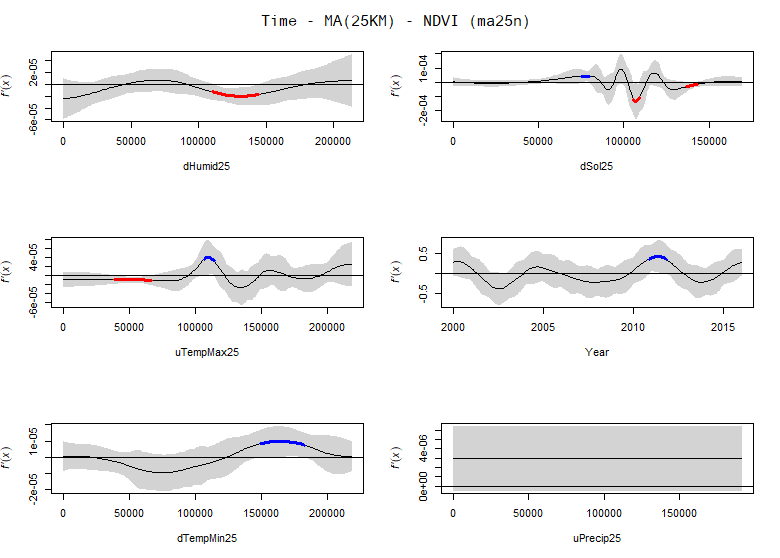
\includegraphics[width=1\textwidth]{ma25n.png} % first figure itself
        \caption{\textbf{Model ma25n}}
    \end{minipage}\hfill
    \begin{minipage}{0.8\textwidth}
        \centering
        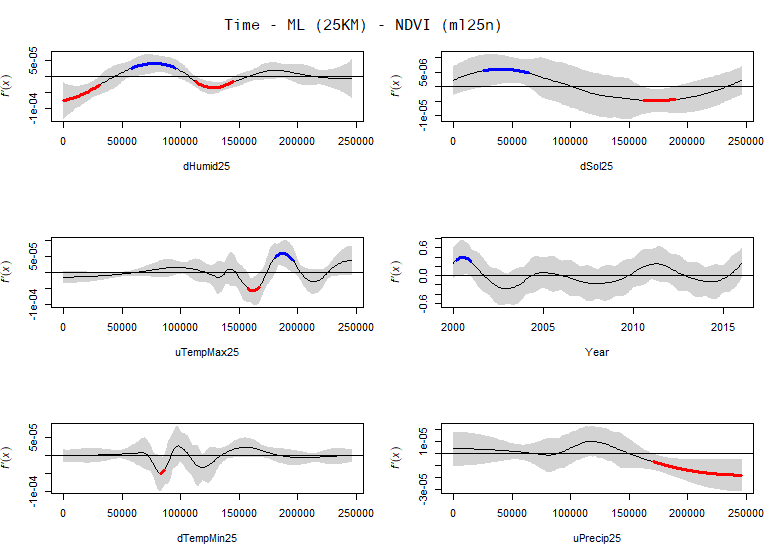
\includegraphics[width=1\textwidth]{ml25n.png} % second figure itself
        \caption{\textbf{Model ml25n}}
    \end{minipage}
\end{figure}

\begin{figure}[H]
 \centering
    \begin{minipage}{0.8\textwidth}
        \centering
        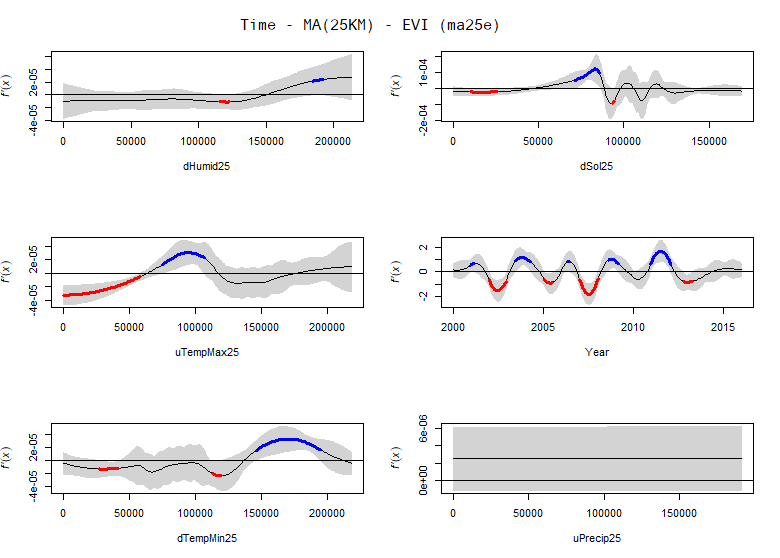
\includegraphics[width=1.2\textwidth]{ma25e.png} % first figure itself
        \caption{\textbf{Model ma25e}}
    \end{minipage}\hfill
    \begin{minipage}{0.8\textwidth}
        \centering
        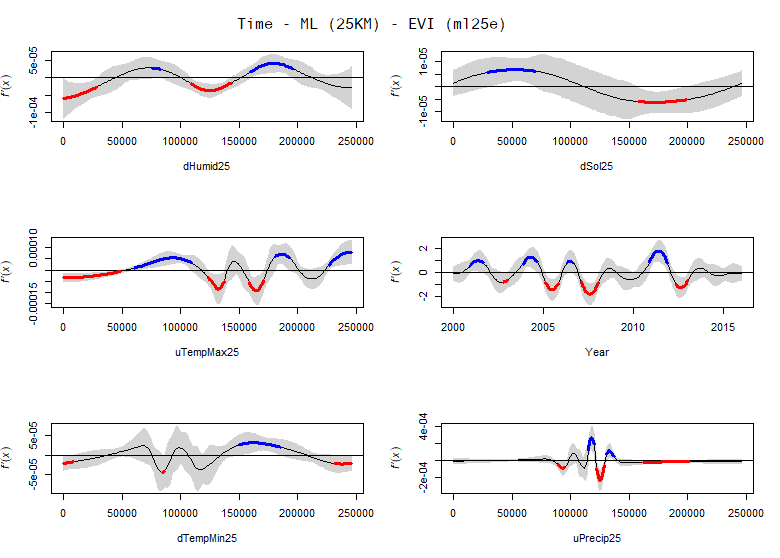
\includegraphics[width=1.2\textwidth]{ml25e.png} % second figure itself
        \caption{\textbf{Model ml25e}}
    \end{minipage}
\end{figure}

\begin{comment}
\begin{figure}[H]

    \begin{minipage}{0.8\textwidth}
        \centering
        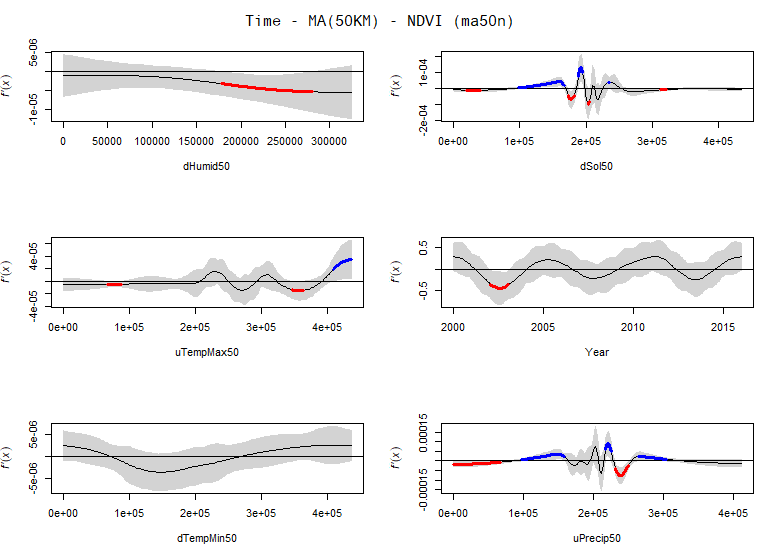
\includegraphics[width=1.2\textwidth]{ma50n.png} % first figure itself
        \caption{\textbf{Model ma50n}}
    \end{minipage}\hfill
    \begin{minipage}{0.8\textwidth}
        \centering
        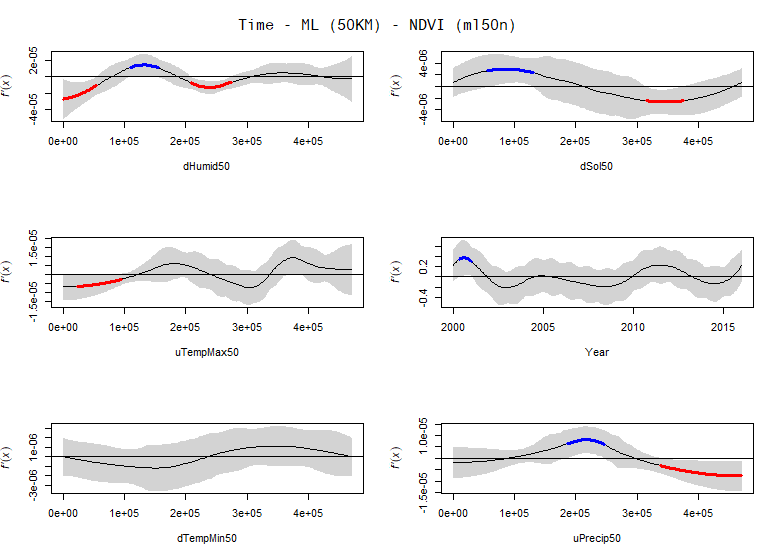
\includegraphics[width=1.2\textwidth]{ml50n.png} % second figure itself
        \caption{\textbf{Model ml50n}}
    \end{minipage}
\end{figure}

\begin{figure}[H]
 \centering
    \begin{minipage}{0.8\textwidth}
        \centering
        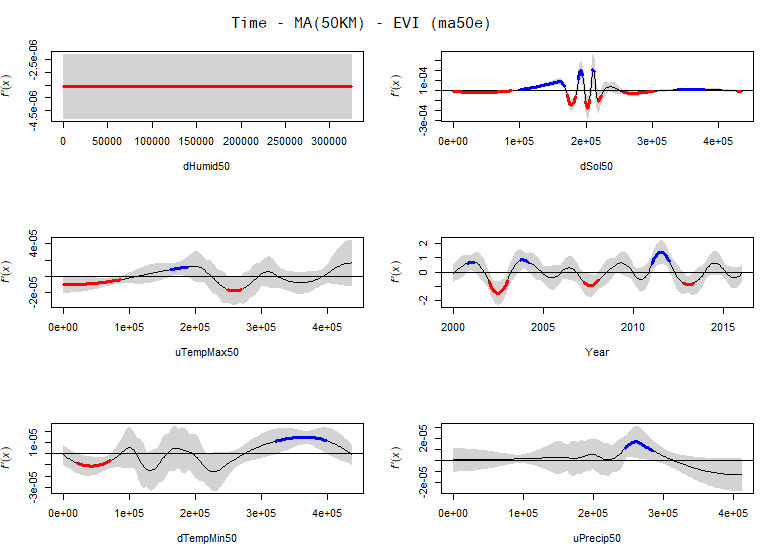
\includegraphics[width=1.2\textwidth]{ma50e.png} % first figure itself
        \caption{\textbf{Model ma50e}}
    \end{minipage}\hfill
    \begin{minipage}{0.8\textwidth}
        \centering
        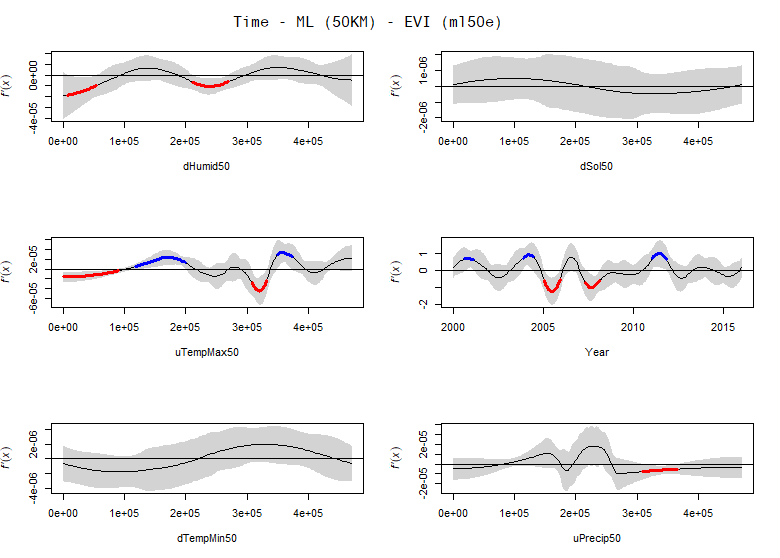
\includegraphics[width=1.2\textwidth]{ml50e.png} % second figure itself
        \caption{\textbf{Model ml50e}}
    \end{minipage}
\end{figure}

\begin{figure}[H]
    \begin{minipage}{0.8\textwidth}
        \centering
        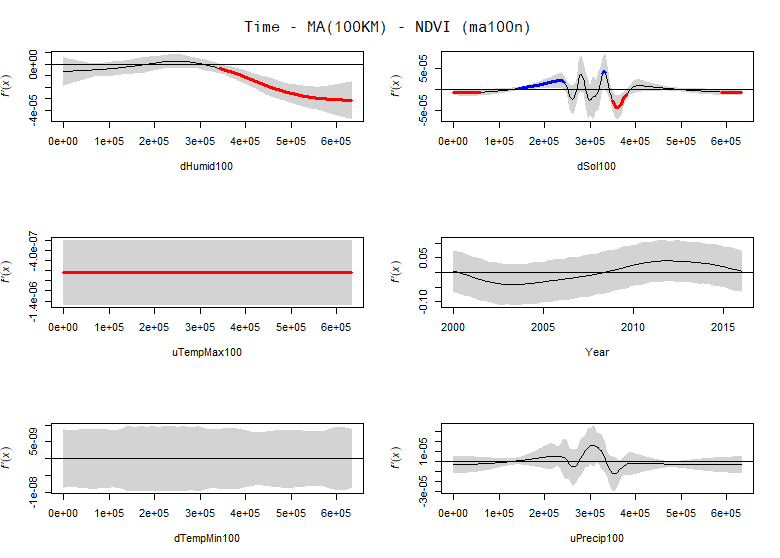
\includegraphics[width=1.2\textwidth]{ma100n.png} % first figure itself
        \caption{\textbf{Model ma100n}}
    \end{minipage}\hfill
    \begin{minipage}{0.8\textwidth}
        \centering
        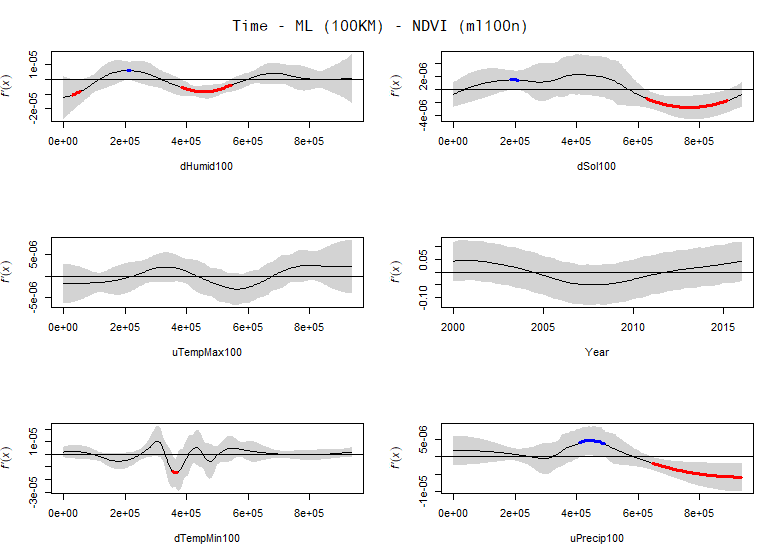
\includegraphics[width=1.2\textwidth]{ml100n.png} % second figure itself
        \caption{\textbf{Model ml100n}}
    \end{minipage}
\end{figure}

\begin{figure}[H]
 \centering
    \begin{minipage}{0.8\textwidth}
        \centering
        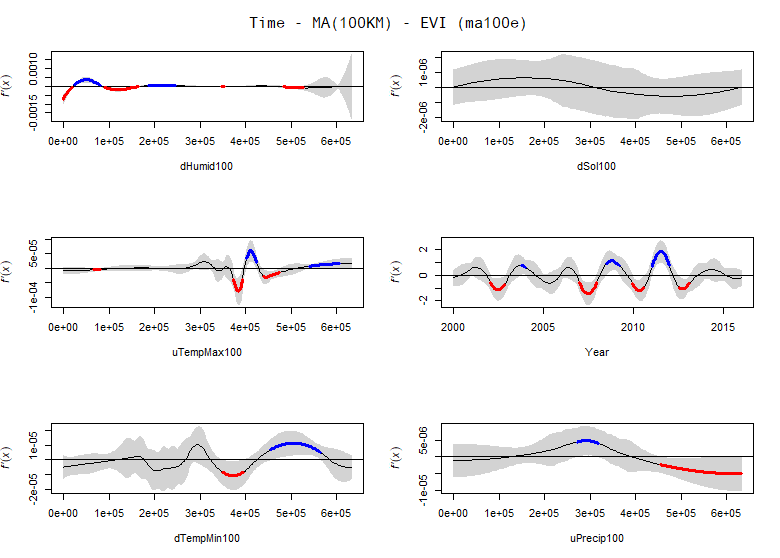
\includegraphics[width=1.2\textwidth]{ma100e.png} % first figure itself
        \caption{\textbf{Model ma100e}}
    \end{minipage}\hfill
    \begin{minipage}{0.8\textwidth}
        \centering
        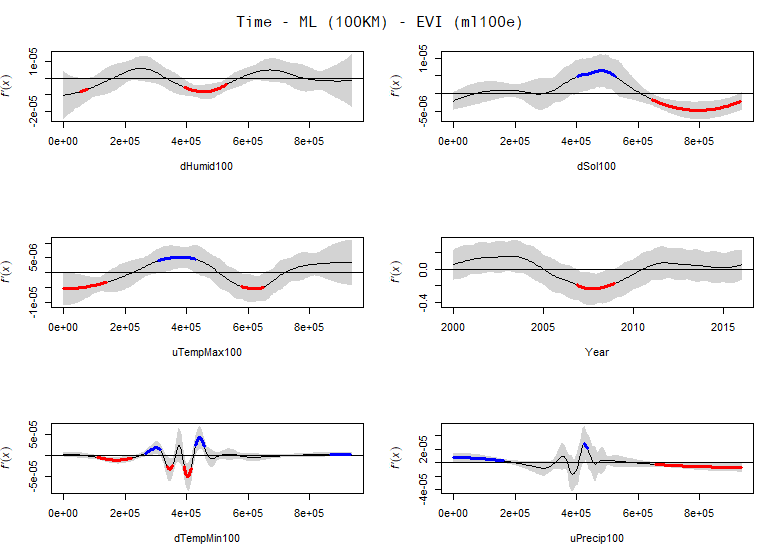
\includegraphics[width=1.2\textwidth]{ml100e.png} % second figure itself
        \caption{\textbf{Model ml100e}}
    \end{minipage}
\end{figure}
\end{comment}

\begin{figure}[H]
 \centering
    \begin{minipage}{0.8\textwidth}
        \centering
        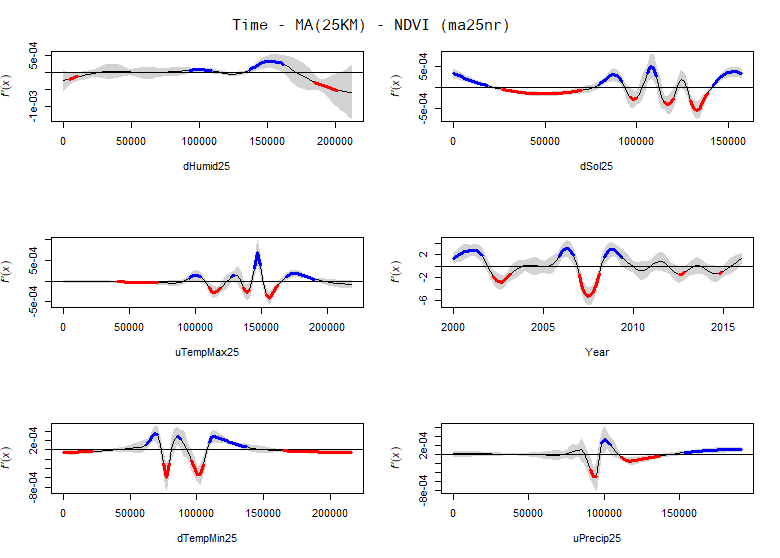
\includegraphics[width=1.2\textwidth]{ma25nr.png} % first figure itself
        \caption{\textbf{Model ma25nr}}
    \end{minipage}\hfill
    \begin{minipage}{0.8\textwidth}
        \centering
        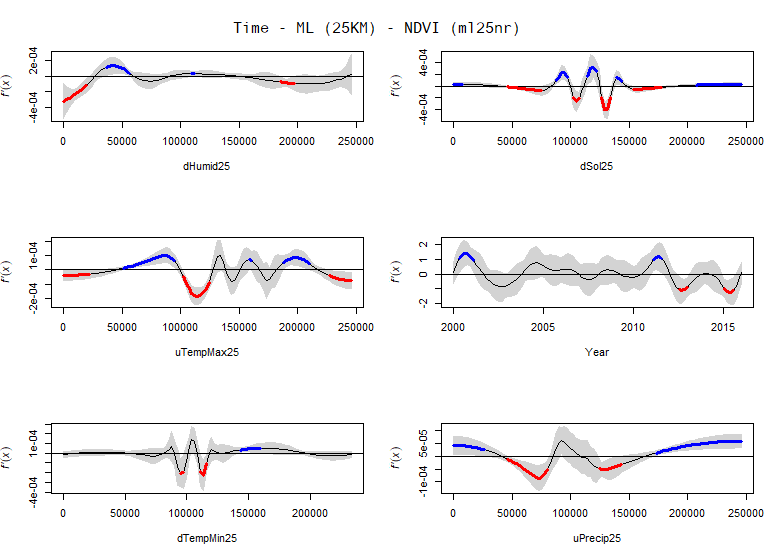
\includegraphics[width=1.2\textwidth]{ml25nr.png} % second figure itself
        \caption{\textbf{Model ml25nr}}
    \end{minipage}
\end{figure}

\begin{figure}[H]
 \centering
    \begin{minipage}{0.8\textwidth}
        \centering
        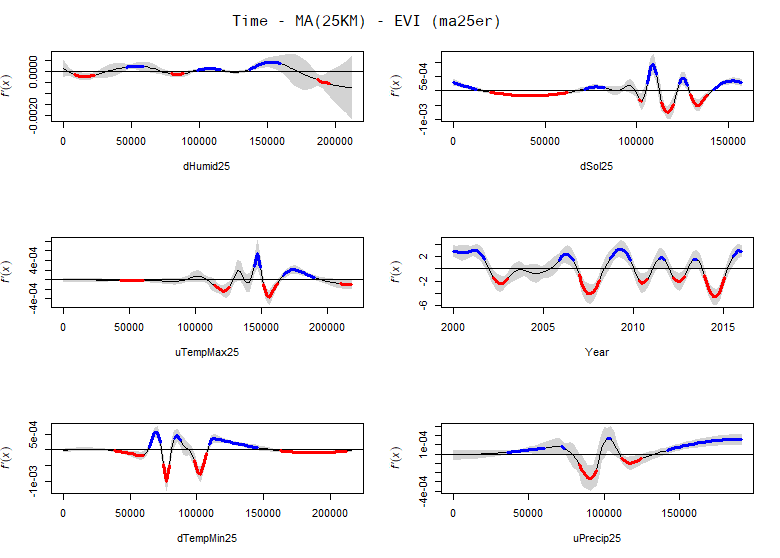
\includegraphics[width=1.2\textwidth]{ma25er.png} % first figure itself
        \caption{\textbf{Model ma25er}}
    \end{minipage}\hfill
    \begin{minipage}{0.8\textwidth}
        \centering
        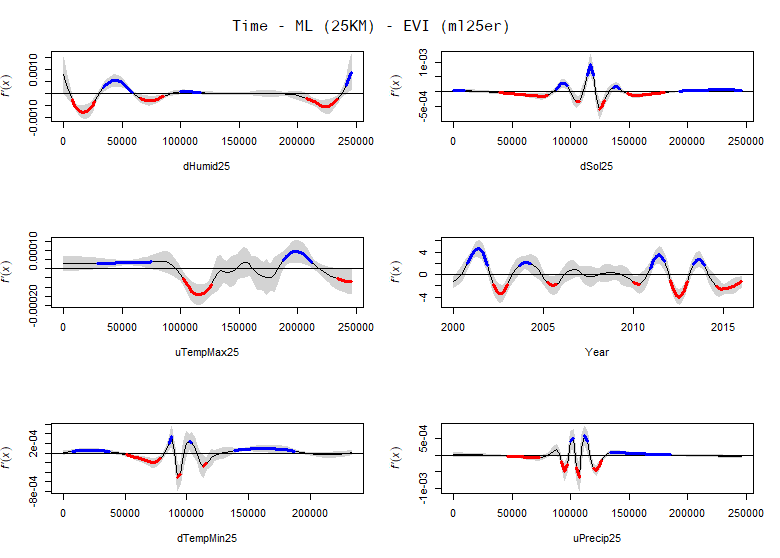
\includegraphics[width=1.2\textwidth]{ml25er.png} % second figure itself
        \caption{\textbf{Model ml25er}}
    \end{minipage}
\end{figure}

\begin{figure}[H]

    \begin{minipage}{0.8\textwidth}
        \centering
        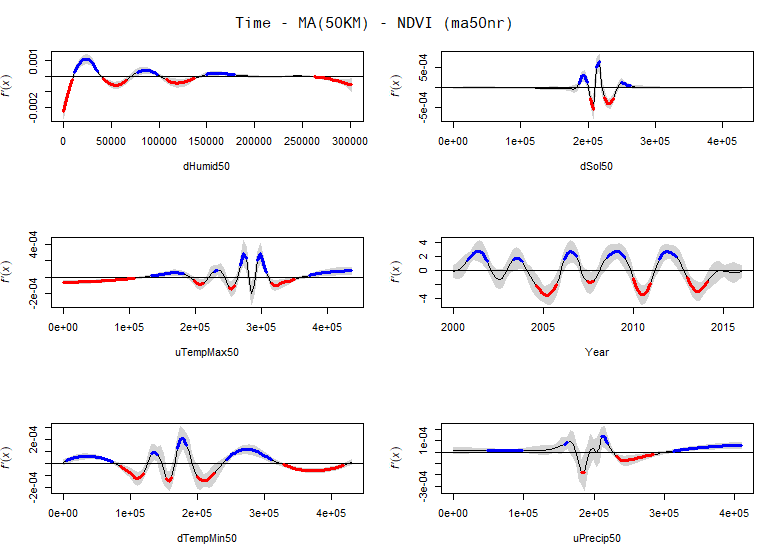
\includegraphics[width=1.2\textwidth]{ma50nr.png} % first figure itself
        \caption{\textbf{Model ma50nr}}
    \end{minipage}\hfill
    \begin{minipage}{0.8\textwidth}
        \centering
        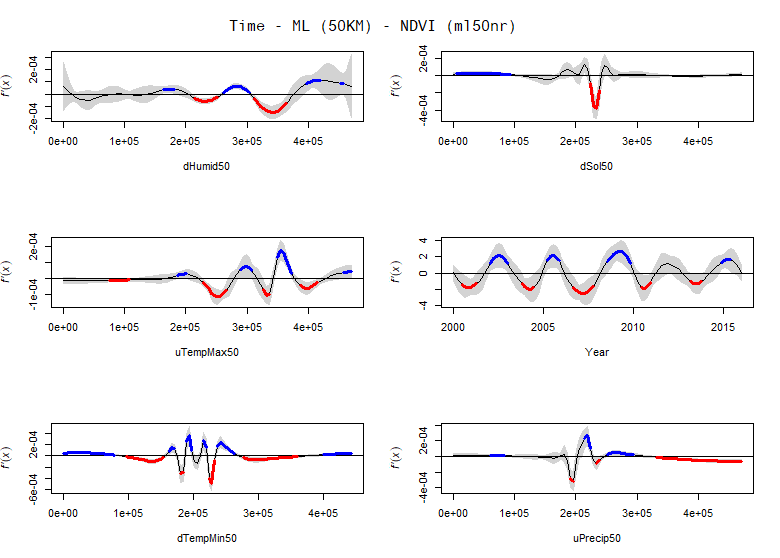
\includegraphics[width=1.2\textwidth]{ml50nr.png} % second figure itself
        \caption{\textbf{Model ml50nr}}
    \end{minipage}
\end{figure}

\begin{figure}[H]
 \centering
    \begin{minipage}{0.8\textwidth}
        \centering
        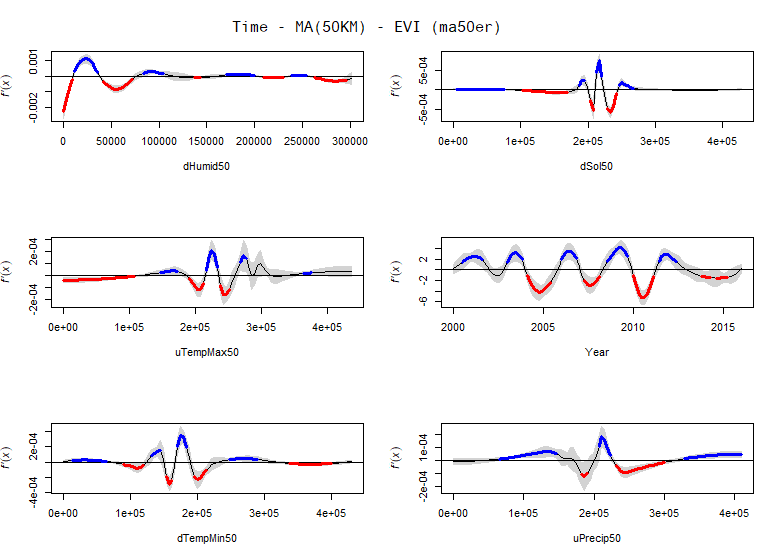
\includegraphics[width=1.2\textwidth]{ma50er.png} % first figure itself
        \caption{\textbf{Model ma50er}}
    \end{minipage}\hfill
    \begin{minipage}{0.8\textwidth}
        \centering
        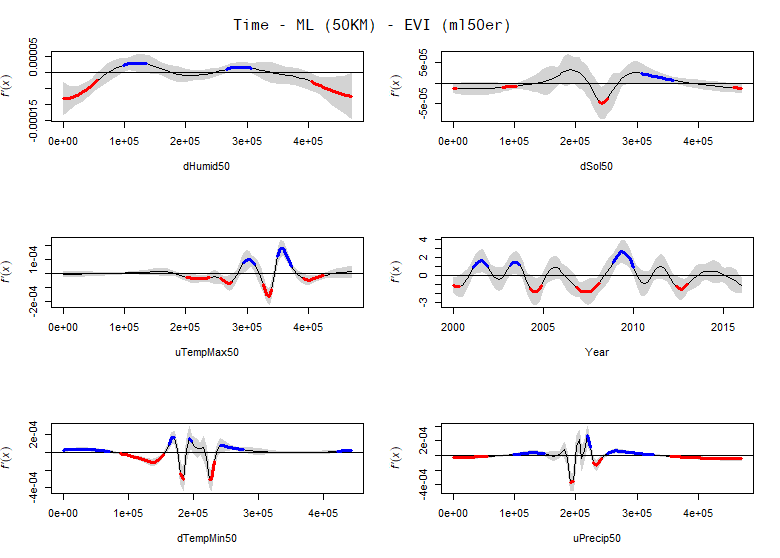
\includegraphics[width=1.2\textwidth]{ml50er.png} % second figure itself
        \caption{\textbf{Model ml50er}}
    \end{minipage}
\end{figure}

\begin{figure}[H]
    \begin{minipage}{0.8\textwidth}
        \centering
        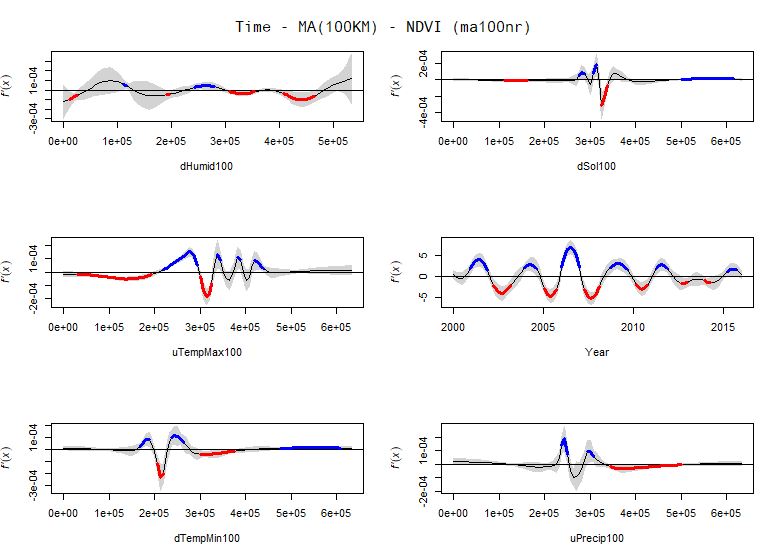
\includegraphics[width=1.2\textwidth]{ma100nr.png} % first figure itself
        \caption{\textbf{Model ma100nr}}
    \end{minipage}\hfill
    \begin{minipage}{0.8\textwidth}
        \centering
        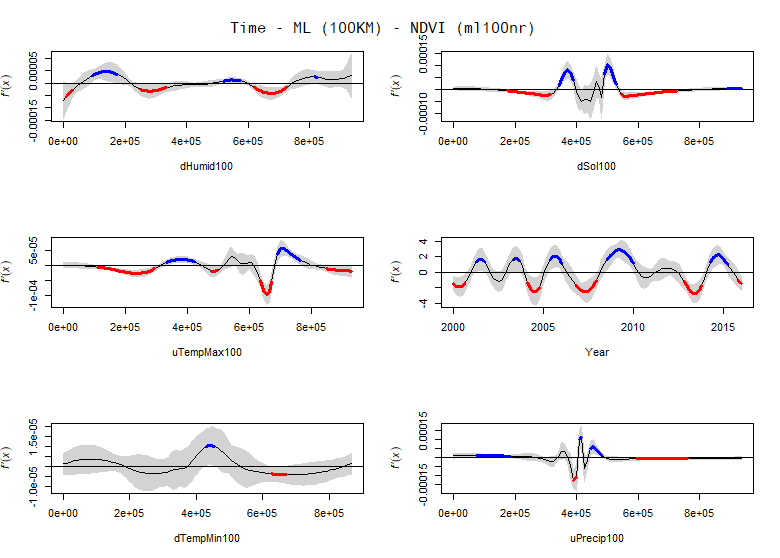
\includegraphics[width=1.2\textwidth]{ml100nr.png} % second figure itself
        \caption{\textbf{Model ml100nr}}
    \end{minipage}
\end{figure}

\begin{figure}[H]
 \centering
    \begin{minipage}{0.8\textwidth}
        \centering
        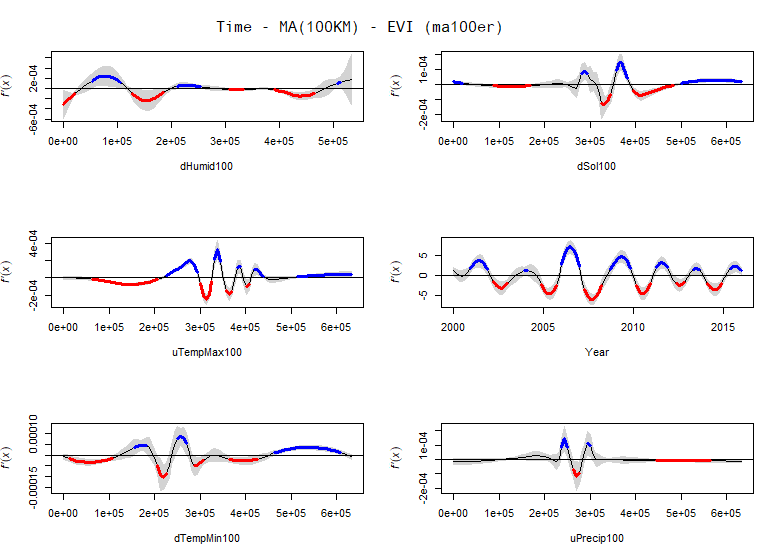
\includegraphics[width=1.2\textwidth]{ma100er.png} % first figure itself
        \caption{\textbf{Model ma100er}}
    \end{minipage}\hfill
    \begin{minipage}{0.8\textwidth}
        \centering
        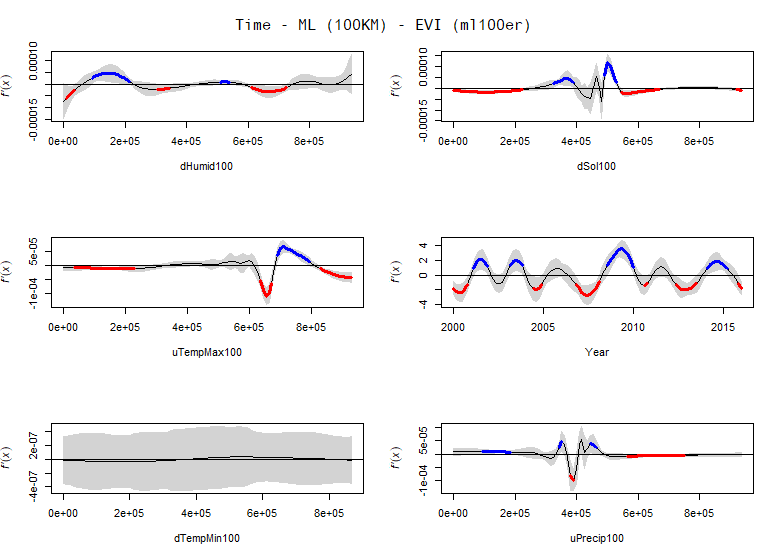
\includegraphics[width=1.2\textwidth]{ml100er.png} % second figure itself
        \caption{\textbf{Model ml100er}}
    \end{minipage}
\end{figure}

\begin{figure}[H]
 \centering
    \begin{minipage}{0.8\textwidth}
        \centering
        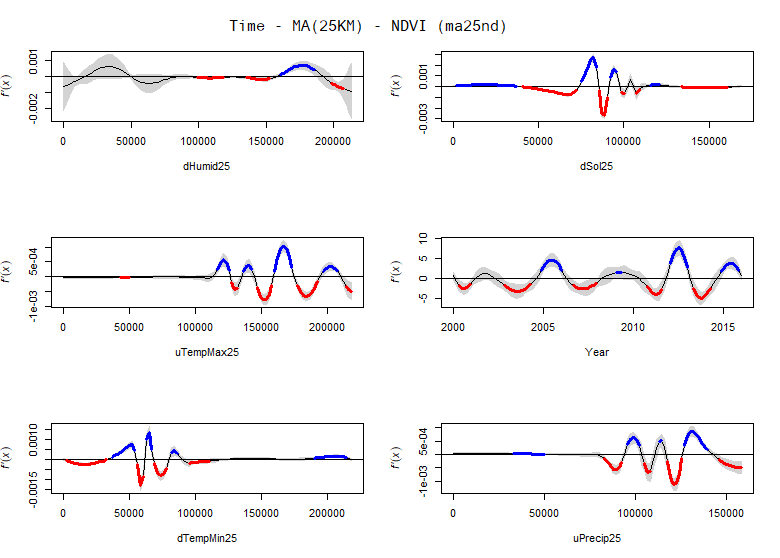
\includegraphics[width=1.2\textwidth]{ma25nd.png} % first figure itself
        \caption{\textbf{Model ma25nd}}
    \end{minipage}\hfill
    \begin{minipage}{0.8\textwidth}
        \centering
        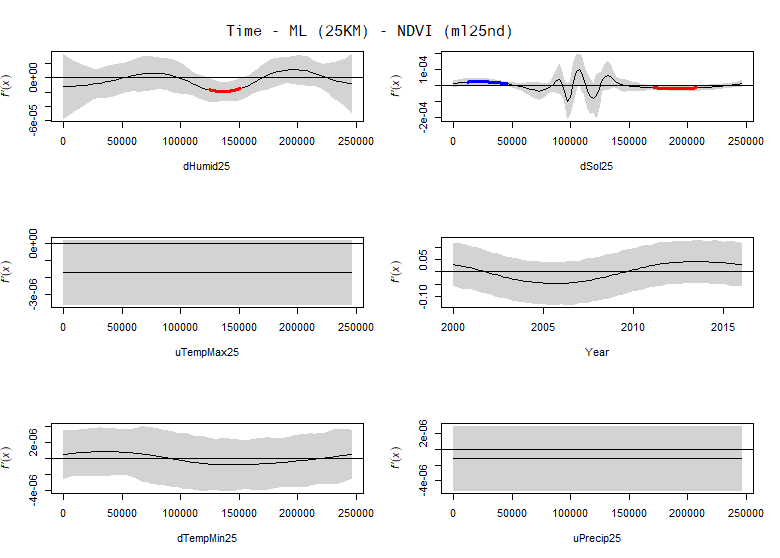
\includegraphics[width=1.2\textwidth]{ml25nd.png} % second figure itself
        \caption{\textbf{Model ml25nd}}
    \end{minipage}
\end{figure}

\begin{figure}[H]
 \centering
    \begin{minipage}{0.8\textwidth}
        \centering
        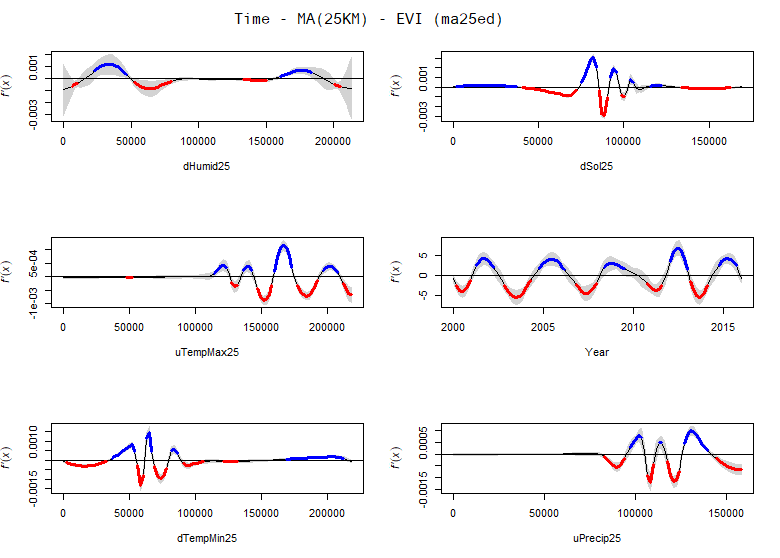
\includegraphics[width=1.2\textwidth]{ma25ed.png} % first figure itself
        \caption{\textbf{Model ma25ed}}
    \end{minipage}\hfill
    \begin{minipage}{0.8\textwidth}
        \centering
        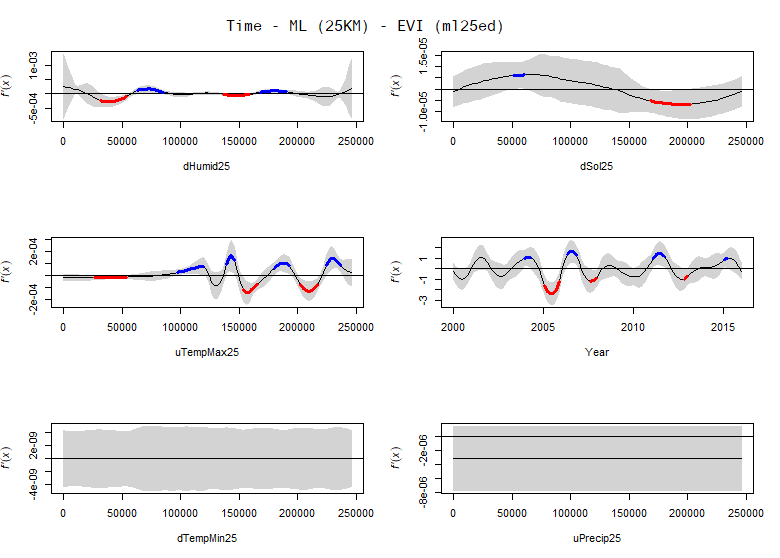
\includegraphics[width=1.2\textwidth]{ml25ed.png} % second figure itself
        \caption{\textbf{Model ml25ed}}
    \end{minipage}
\end{figure}

\begin{figure}[H]

    \begin{minipage}{0.8\textwidth}
        \centering
        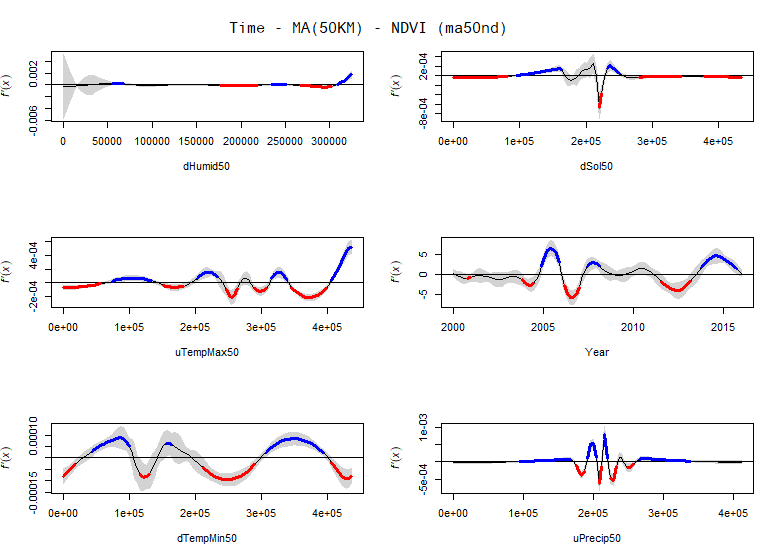
\includegraphics[width=1.2\textwidth]{ma50nd.png} % first figure itself
        \caption{\textbf{Model ma50nd}}
    \end{minipage}\hfill
    \begin{minipage}{0.8\textwidth}
        \centering
        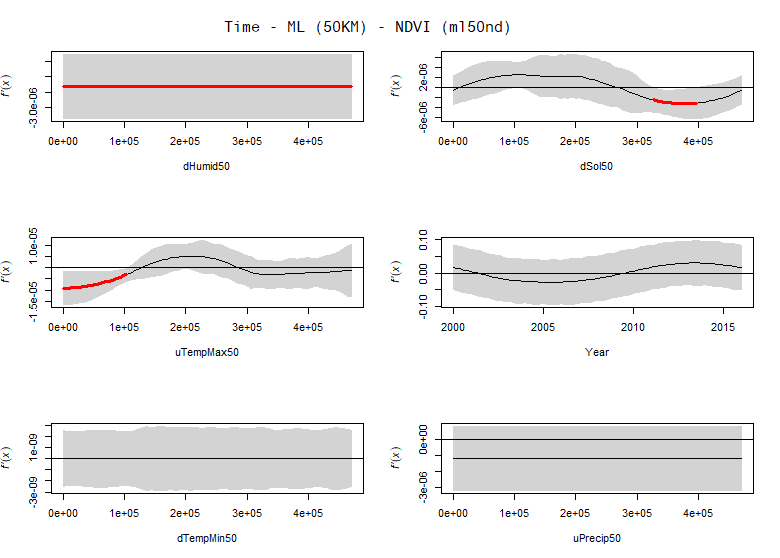
\includegraphics[width=1.2\textwidth]{ml50nd.png} % second figure itself
        \caption{\textbf{Model ml50nd}}
    \end{minipage}
\end{figure}

\begin{figure}[H]
 \centering
    \begin{minipage}{0.8\textwidth}
        \centering
        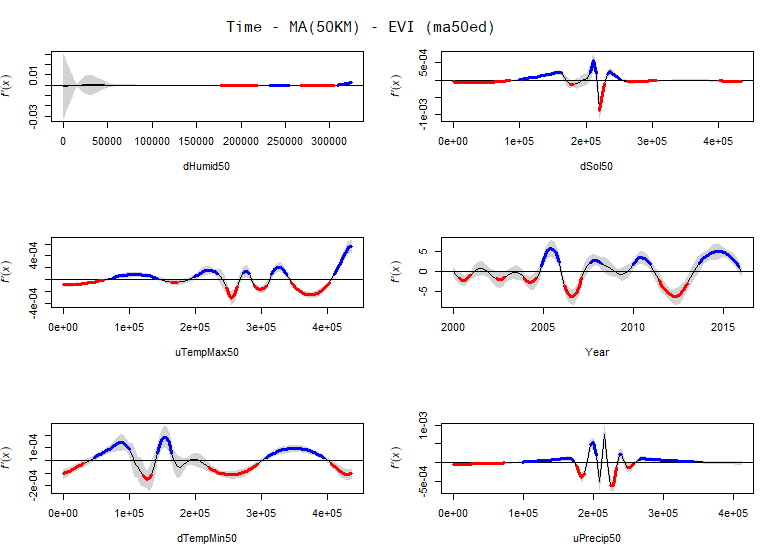
\includegraphics[width=1.2\textwidth]{ma50ed.png} % first figure itself
        \caption{\textbf{Model ma50ed}}
    \end{minipage}\hfill
    \begin{minipage}{0.8\textwidth}
        \centering
        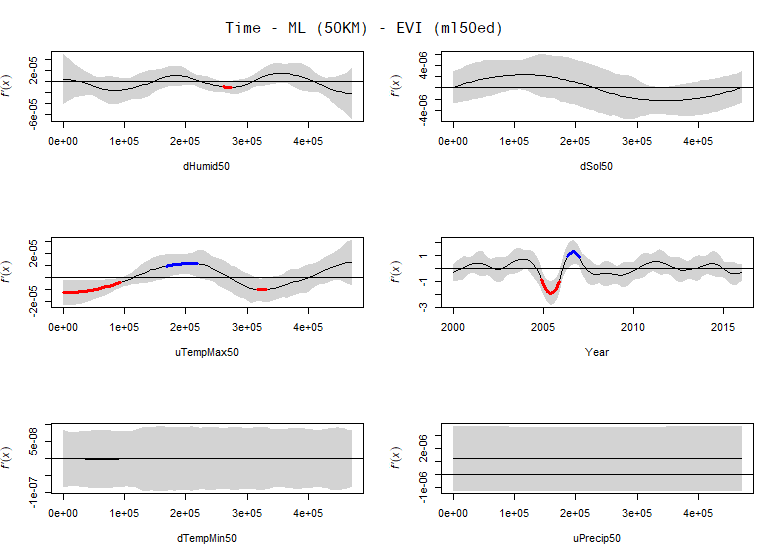
\includegraphics[width=1.2\textwidth]{ml50ed.png} % second figure itself
        \caption{\textbf{Model ml50ed}}
    \end{minipage}
\end{figure}

\begin{figure}[H]
    \begin{minipage}{0.8\textwidth}
        \centering
        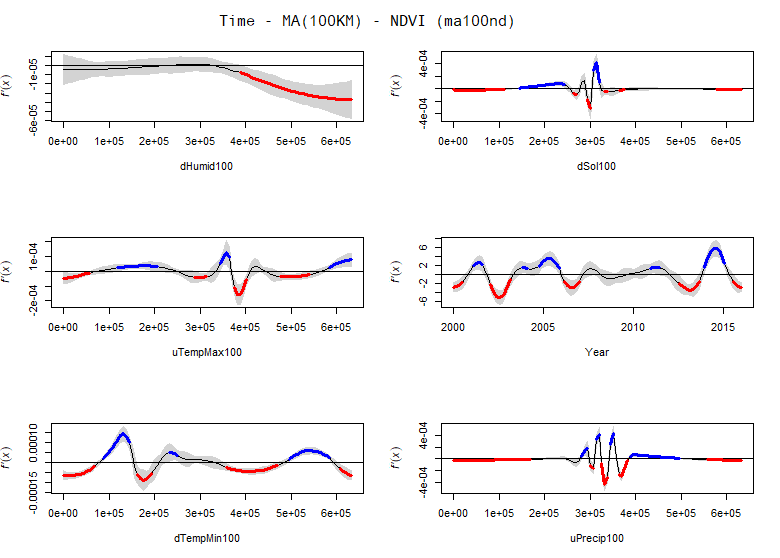
\includegraphics[width=1.2\textwidth]{ma100nd.png} % first figure itself
        \caption{\textbf{Model ma100nd}}
    \end{minipage}\hfill
    \begin{minipage}{0.8\textwidth}
        \centering
        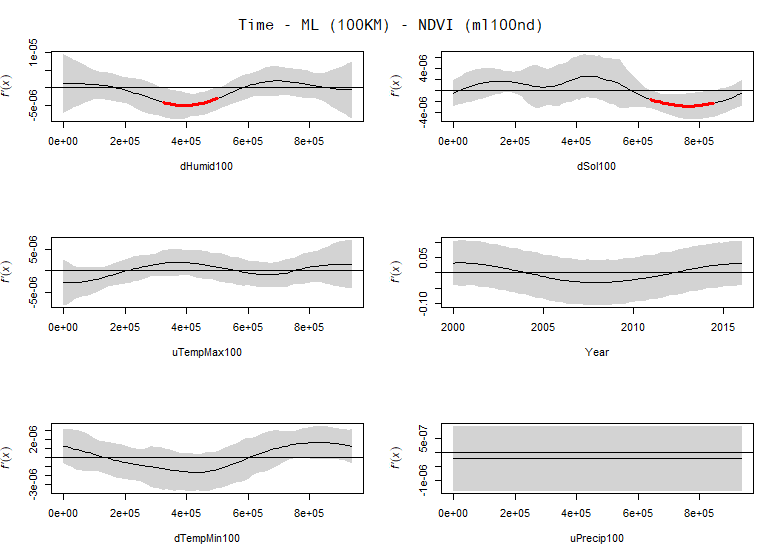
\includegraphics[width=1.2\textwidth]{ml100nd.png} % second figure itself
        \caption{\textbf{Model ml100nd}}
    \end{minipage}
\end{figure}

\begin{figure}[H]
 \centering
    \begin{minipage}{0.8\textwidth}
        \centering
        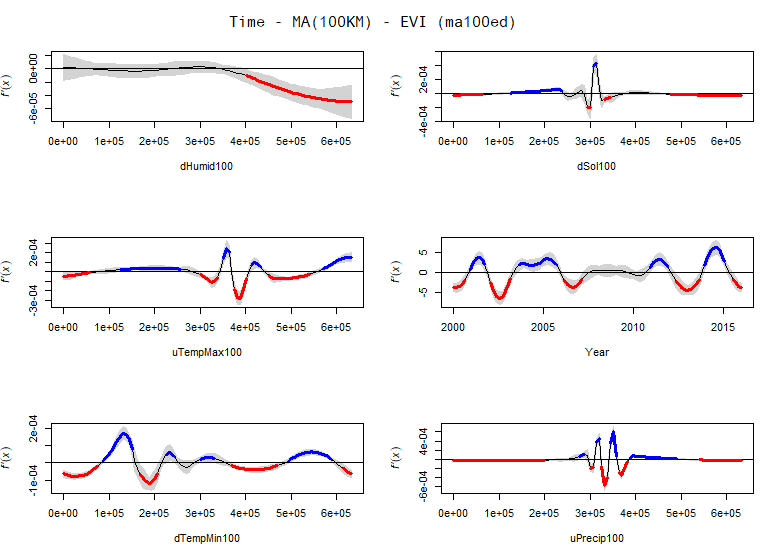
\includegraphics[width=1.2\textwidth]{ma100ed.png} % first figure itself
        \caption{\textbf{Model ma100ed}}
    \end{minipage}\hfill
    \begin{minipage}{0.8\textwidth}
        \centering
        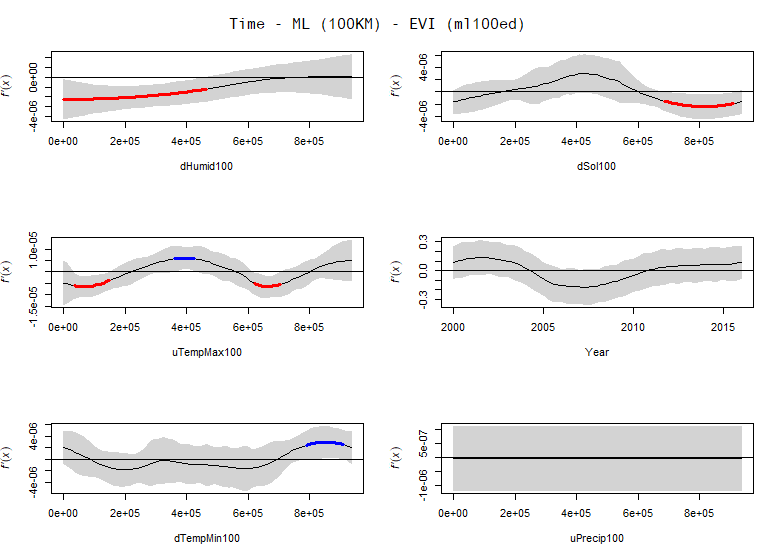
\includegraphics[width=1.2\textwidth]{ml100ed.png} % second figure itself
        \caption{\textbf{Model ml100ed}}
    \end{minipage}
\end{figure}


\begin{figure}[H]
  \centering
  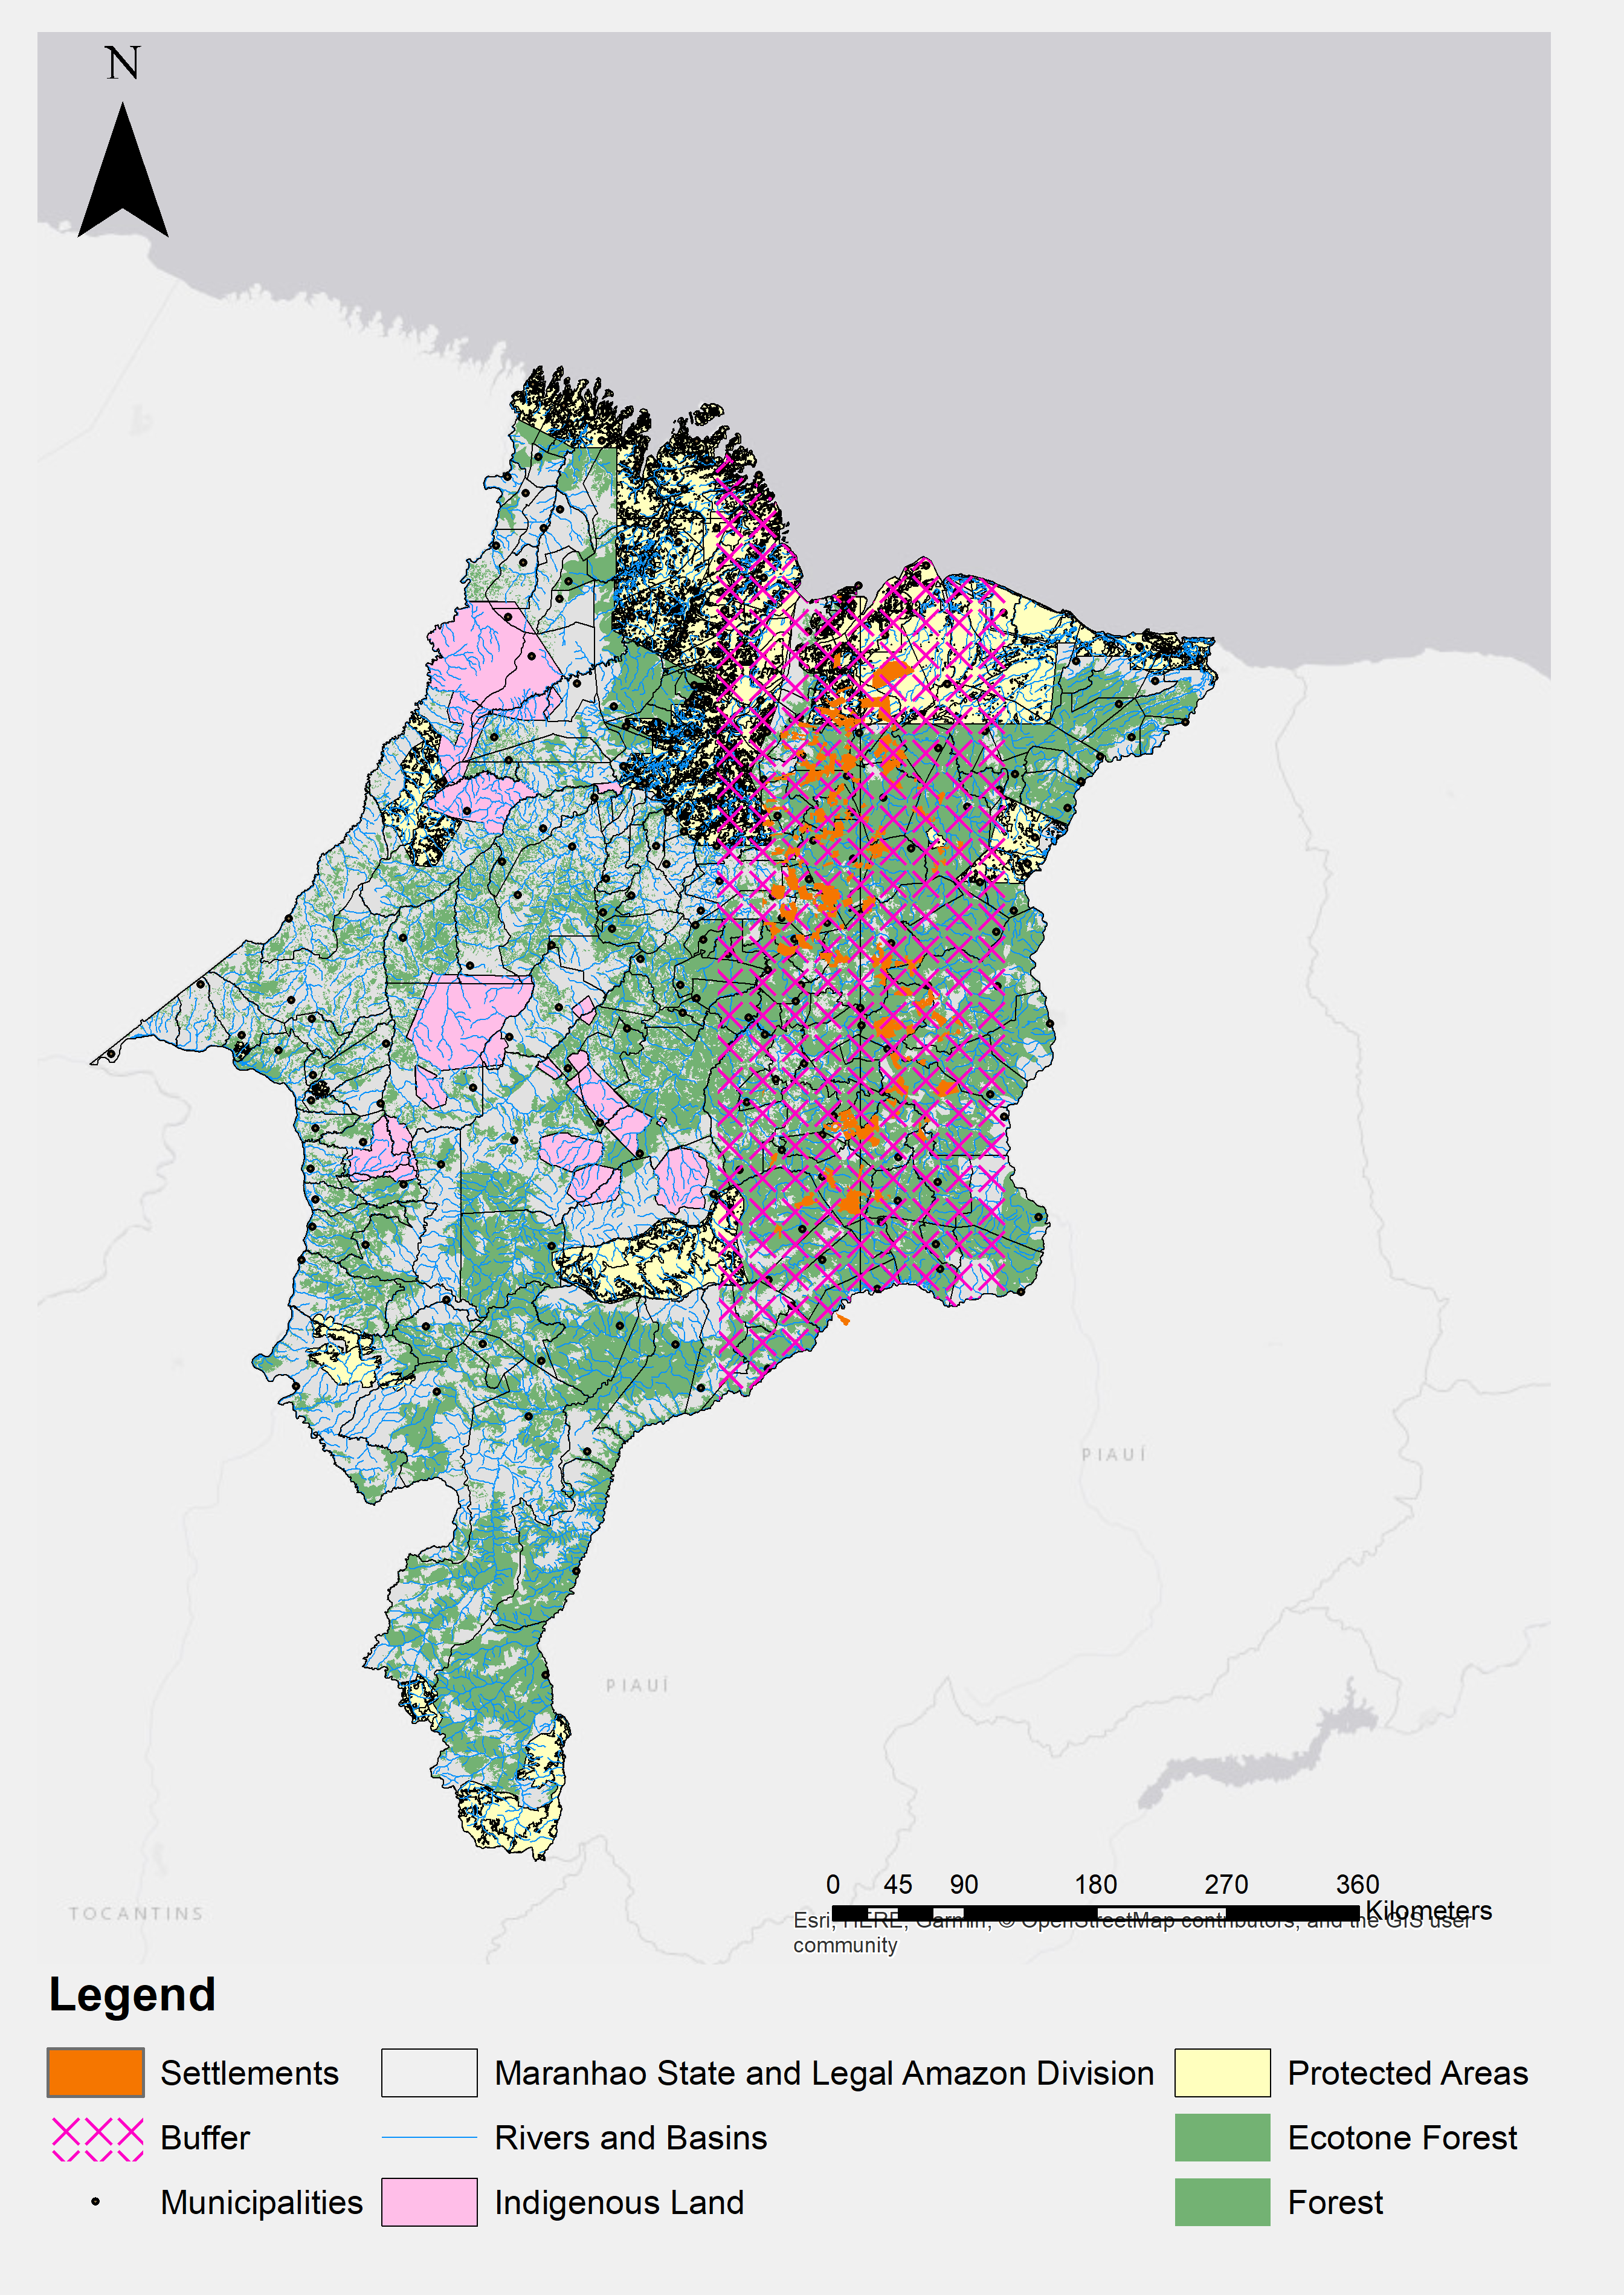
\includegraphics[width=1\textwidth, inner]{Chapter2/MaranhaoChapter2_Fig3.png}
\caption{Source: \citep{MMMAwebsite,nugeo_2018,embrapa_2018, INCRA}.}
\label{fig:delimitacaosett}
\end{figure}

\begin{landscape}
\begin{figure}[H]
  \centering
  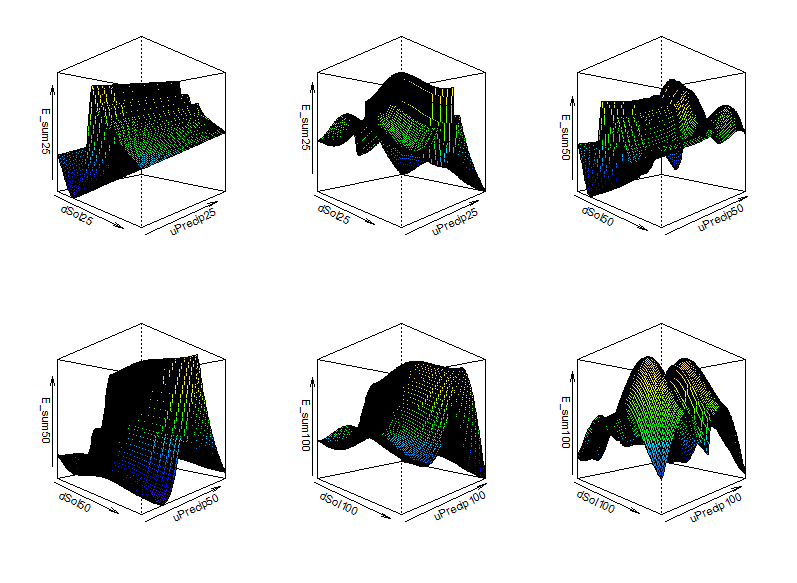
\includegraphics[width=1.5\textwidth, inner]{visgam.png}
\caption{\textbf{Interactions between selected variables for the baseline model.}}
\label{fig:visgam}
\end{figure}



\begin{figure}[H]
  \centering
  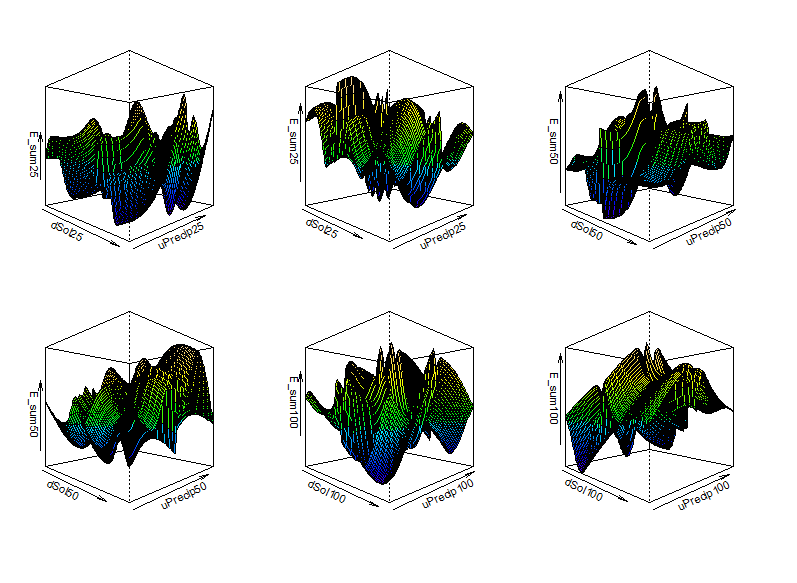
\includegraphics[width=1.5\textwidth, inner]{visgamr.png}
\caption{\textbf{Interactions between selected variables for the rain season model.}}
\label{fig:visgamr}
\end{figure}


\begin{figure}[H]
  \centering
  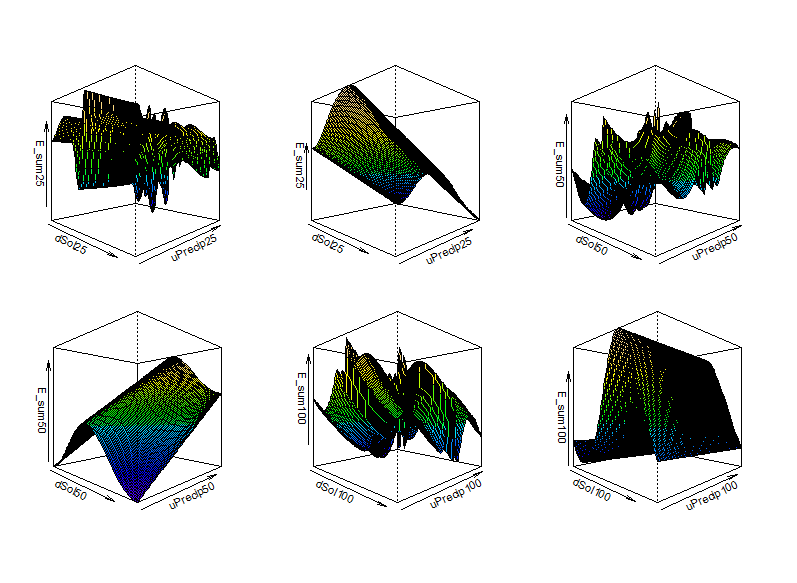
\includegraphics[width=1.5\textwidth, inner]{visgamd.png}
\caption{\textbf{Interactions between selected variables for the dry season model.}}
\label{fig:visgamd}
\end{figure}


\begin{figure}[H]
  \centering
  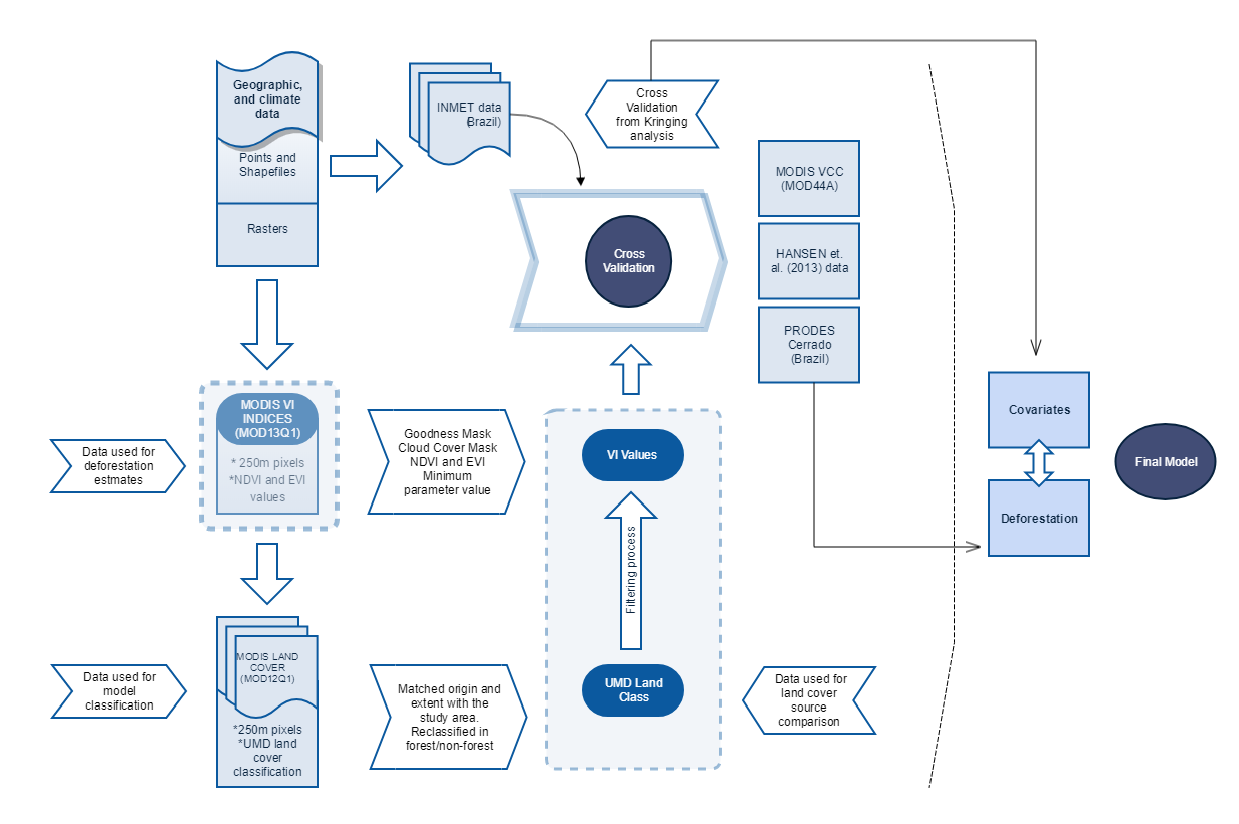
\includegraphics[width=1.5\textwidth, inner]{method.png}
\caption{\textbf{Flowchart of method applied to data}. Moving from left to right indicates increasing levels of data processing during the study.}
\label{fig:method}
\end{figure}
\end{landscape}

\end{appendices}

%!TEX root = ../thesis.tex
%*******************************************************************************
%****************************** Third Chapter **********************************
%*******************************************************************************
\chapter{Satellite Monitoring of Deforestation and the Role of Clouds in Maranhão}

% **************************** Define Graphics Path **************************
\ifpdf
    \graphicspath{{Chapter3/}}
\else
    \graphicspath{{Chapter3/}}
\fi

\begin{abstract}
Deforestation rates in Brazil have declined noticeably over the past decade and it is believed that  environmental policies used as instruments to encourage forest preservation have played a crucial role in this trend. In particular, the satellite monitoring program has enabled authorities to identify and react to deforestation in a much more timely manner than local field detection.  However, importantly, cloud coverage, by delaying detection until skies are clear, has potentially acted as an important impediment to the policy's success. To investigate this we use satellite data within a survival analysis.  Focusing on the ecological tension zone of Maranhão that is separated into two parts by an artificial line- one that was covered by environmental deforestation policy and the other that is not subject to this - we estimate how the probability of transition between intact forest to disturbed forest, given risk factors and conditional on the time elapsed until the occurrence of the transition, is affected by cloud coverage. The results suggest that the presence of clouds has increased deforestation in the region covered by the satellite detection program, and thus is likely an active barrier to legal compliance.  

\noindent{\bf Keywords: Remote Sensing, Survival Analysis, Environmental Policies, Deforestation} 

\end{abstract}

\section{Introduction}
\label{S:3.1}
%Describing policies that decreased the rate of deforestation in Brazil
The clear-cutting of forests plays a central role in many environmental threats of our time, including global climate change, habitat degradation, and species extinction. Reassuringly, deforestation rates in Brazil have declined over the past decade, and it is generally believed that an important reason for this reduction has been environmental policies used as instruments to encourage forest preservation \citep{NEPSTAD, RICHARDS, RICHARDS2, CELENTANO_2017}. The best example in this regard is the satellite monitoring program that has allowed the Brazilian environmental police to considerably speed up their response to punish clear-cutting agents by detecting local deforestation remotely and much quicker than through local inspection. More specifically, in 2004, the Brazilian government created the Action Plan for the Prevention and Control of Deforestation in the Legal Amazon (PPCDAm in Portuguese), where the purpose of this program was to plan development, control land use and ensure compliance with the environmental law and promote sustainable practices. In order to control land use and prevent further deforestation, the PPCDAm importantly included two satellite-based monitoring programme PRODES (Programa de Cálculo do Desflorestamento da
Amazônia in Portuguese) \citep{inpe} that recorded the annual rate of deforestation within the policy area using fine resolution, and the DETER (Sistema de Detecção de Desmatamento em Tempo Real in Portuguese) programme, which is a system to support the supervision and control of deforestation in the Amazon in a coarse resolution throughout the year within the environmental policy area. DETER reports deforestation alerts on areas, greater than 250m, in the process of deforestation by degradation forest management to fully deforested areas (shallow cut).\footnote{In order to control for degradation of the forest by selective logging and forest fires, the government uses the DETER program. In addition, two other systems were introduced in 2007: DEGRAD (Mapeamento da Degradaç\~{a}o Florestal na Amaz\^{o}nia Brasileira in Portuguese), for mapping forest degradation in the Legal Amazon, and DETEX (Mapeamento da Cobertura Florestal na Amaz\^{o}nia Brasileira in Portuguese), for detecting logging operations in the Legal Amazon region \citep{VALERIANO}. In order to control land use and prevent further deforestation, the PPCDAm  also includes the satellite-based monitoring programme PRODES (Projeto de Estimativa do Desflorestameno da Amaz\^{o}nia in Portuguese) \citep{inpe} that attempts to record incidents of deforestation throughout the year within the policy area. All the data gathered by the action plan are used to enforce the PPPCDAm plan, which includes the issuing of fines for agents who clear or damage the forest, embargoes of areas in the process of being cleared with the confiscation of equipment, and restrictions on access to subsidised credit \citep{AUBERTIN}.}



While DETER has certainly allowed much quicker detection of local deforestation, an important impediment to its success has been local climate.  More specifically, because the satellite used is incapable of detecting land cover changes when its view of land is obscured by clouds, detection will be delayed until skies are clear again.  As a matter of fact, \cite{ASSUNCAO_2017} show that cloud coverage is an important predictor of the extent of deforestation fines issued within municipalities in the Brazilian amazon.  This may not be surprising since, according to \citet{VALERIANO, ASSUNCAO_2017}, Brazil's institutional setup is such that law enforcement agents can more easily punish offenders for illegal forest clearings when catching them red-handed, since offenders can thereby be held directly accountable for the crime. That is, although in principle Brazilian past deforestation acts can be legally punished, this is difficult to implement ex post in the Amazon, where land and production property rights are unclear. Moreover, once deforestation has already occurred, the absence of well-defined property rights makes it very difficult or even impossible to identify who owns the cleared land, so that sanctions or punishment becomes pointless if no one can be held responsible for the crime. Not to mention that accessing these cleared areas requires substantial efforts since illegal roads are built under precarious way \citep{PFAFF3}. Additionally, there is considerable evidence of corruption among local government officials who monitor and fine loggers. Furthermore, some firms can exert political influence to obtain favourable terms and often bribe government officials during the concession process to overlook noncompliance. The reason for this ranges from underpaid inspectors, potentially high rents to resource stocks, and low penalties and lack of enforcement by centrally located governments in open access distant native forests \citep{amacher_2012}.

Despite the potentially crucial importance of cloud coverage in deterring the detection of deforestation through the DETER satellite program, there is no study that explicitly examines this.\footnote{\cite{ASSUNCAO_2017} do use cloud coverage as an instrumental variable to identify how deforestation fines have affected deforestation across municipalities in the Brazilian Amazon.  However, their implied estimate of the impact of fines on deforestation through cloud coverage can only be viewed as capturing the effect of clouds partially and very roughly.  Firstly, the cloud coverage will have affected other aspects of deforestation through other legal coercion such confiscation of assets or access to credit and commercialisation channels; see \citep{borner2015post}.  Moreover, since their analysis undertaken at the municipality level, where as satellite detection is at the 250m level, i.e., at the resolution of the satellite images.}  The current paper thus sets out to explicitly quantify the effect of cloud coverage on local levels of deforestation in the Brazilian Amazon. To this end we focus on the ecological tension zone of Maranhão because it is divided by an artificial line that separates it in two parts: the Legal Amazon Maranhão and the Cerrado Maranhão.\footnote{Importantly, in July 2018, the National Institute of Spatial Research (INPE in Portuguese) together with several other institutions published a dataset covering annual and biannual of Cerrado biome deforestation at state and national level. From the dataset, it is shown that deforestation in great Cerrado Maranhão, which includes the transitional forest, has been two times higher than in the Amazon region of Maranhão.} This division, occurring approximately 44$^{\circ}$ west of the meridian, allows the state to be divided in terms of environmental policies, providing us with a spatial division for which the effect of cloud coverage is likely to be very different.  More precisely, unlike forests in the Legal Amazon Maranhão,  Cerrado Maranhão was not under the satellite monitoring program and thus clouds should play no direct role in deforestation other than for climatic reasons. Importantly, the area on both sides of the border is homogeneous in several aspects such as biota, institutions, and, climate,  with the only difference being the surveillance environmental program that is observed in only one part of the region. This provides us with a unique context within which to examine the role of cloud coverage in deforestation, in that we can compare regions that biologically homogeneous but heterogeneous in terms of deforestation detection policy.  To identify local deforestation and cloud coverage within our two regions we use remote sensing sources (MODIS Vegetation Indices (MOD13Q1) product) to construct a time event dataset at the individual pixel level (250m). We then use survival estimation methods to quantify the role of cloud coverage in local deforestation across these two region.    

%Unfortunately, the decline in forest clearing rates observed between 2005 and 2012 now appears to have halted in that the average deforestation rate between 2013 and 2017 was 38\% higher than in 2012, i.e., the year with the lowest rate since the start of measurements. Arguably, this increase in deforestation after 2012 occurred because the risk of punishment and losses associated with the crime of deforestation proved to be low throughout the years. \footnote{Between 2008 and 2013, only 18\% of the total deforested area was seized - given that, in the same period, almost 95\% of the deforestation in the Amazon was illegal.} More specifically, loggers realized that the prosecution concerning infractions was slow and most of the fines were not enforced \citep{moutinho2017}.




% Any empirical evaluation of the Brazilian, or any other country's, forest law enforcement policies has to deal with the fact that enforcement operations are not randomly allocated in space. In the Brazilian case the environmental police inspections tends to concentrate where deforestation has historically been high, i.e. inspections may reduce deforestation, but deforestation also results in higher inspection rates. Many studies have tried to explicitly address this problem of selection bias. For example, \citet{hargrave_kis-katos_2012} address the endogeneity of policy implementation by two complementary instrumental variables strategies: using state level inspection intensity to instrument for municipal inspections, and instrumenting changes in environmental fining intensity with past levels of deforestation and environmental fines in a dynamic panel framework. \citet{Andam2008} evaluated the effectiveness of protected areas, which tend to be intentionally located in remote places with below average deforestation pressure. In contrast, \citet{amacher_2012} minimized the risk of unobservable bias by drawing on a comparatively large set of biophysical, socioeconomic, and spatial covariates that included variables known to influence the spatial allocation of environmental law enforcement operations by the environmental police (IBAMA). More recently, \citet{ASSUNCAO_2017} exploited the fact that the spatial allocation of the environmental police inspections was correlated with cloud cover and, the authors estimated the effect of inspections in an instrumental variable approach.


%Border issue 
%\citet{burgess_costa_olken_2018} showed the differences of deforestation rate at the Brazilian international border. According to their results, the differences were higher and significant until 2006 in the Brazilian portion, right after the implementation of the satellite environmental policy. After that period, the differences disappeared. Although the results lead to a significant positive impact from the policy, it is important to understand these differences \textit{within} Brazilian biomes borders since the rates are a constant risk to the environment and to the increasing concerns on climate change.

%Linking Chapter 2 %Cloud issue 
%A recent study (see Chapter 2) observed the trends of deforestation in two regions, under different environmental policies, of an ecological tension zone (ecotone forest) in Maranhão.\footnote{Ecotone is defined as the transition area between two or more distinct habitats or ecosystems, which may have characteristics of both or their own. Secondary Vegetation includes the various stages of natural succession in areas where there was human intervention for land use, whether for mining, agricultural or livestock purposes, or discharging the primary vegetation \citep{SANTOS-FILHO_2013}.} For the environmentally regulated region, deforestation process shifted from dry season to raining season. Besides that, the study indicated that part of deforestation displaced to the region not controlled by the environmental policy. Apparently, the policy faded in areas of biome transition that coincided with the delimitation of the surveillance policy. In addition, behaviour changes might have emphasised this problem. Event history analysis could confirm these findings by considering the heterogeneity within the region because not all sites within ecological tension zone have the same risk of deforestation. 

%\citet{Vina_2004} investigated the rates and patterns of land-cover change along a portion of the Colombia-Ecuador border during a 23-yr period using satellite data to document the rates. Satellite change detection analysis showed that the annual rates of deforestation were considerably higher for the Colombian side of the border. \citet{Chicas_2017}  studied the trans-boundary deforestation history and patterns in protected areas along the Belize-Guatemala border and indicated that failure to integrate buffer communities, coordinate among managing organisations and establish strong bi-national collaboration has resulted in continued ecological and environmental degradation. 

%Existing Related Literature of Survival Analysis and Deforestation in Borders - Not found. :(
%\citet{Egler_2013} conducted a study in an extensive rain forest-savanna ecotone, located in the south border of Amazon biome showed a significant reduction in production and commercialisation of extractive products in the region. In his work, land use, socioeconomic and conservation indicators, combined with statistical analysis, were used to understand forces associated with patterns of deforestation. The author revealed that the main conservation policy in Mato Grosso was the creation of protected areas. 

There are already a number of other studies that use satellite data to examine the factors driving deforestation.  For example, \citet{vance_2002} estimated a spatially explicit model of forest clearance process in the southern Mexico implementing a time event analysis to identify the effect of households on the probability of deforestation. The results showed a non-linear probability of forest clearance. \citet{greenberg_2005} assessed the impact of spatial, cultural and economic factors on deforestation using survival analysis on satellite data from eastern Ecuador. Their results showed that deforestation prediction was higher when there was proximity to roads. Until now, however, studies combining satellite data in areas of ecotone forest to detect time event (survival) analysis of the risk of deforestation process remains scarce in the Brazilian literature.\footnote{Monitoring the transitional biome is difficult due to the high heterogeneity of the forests (open and dense forest, for example) which are substantially influenced by the climatic seasonality \citep{bayma_sano_2015}. Also, there is no environmental policy in place to prevent rampant deforestation. However, in the context of the Amazon region which is under a specific environmental policy, it is arguably crucial to understand the dynamic of the transitional forest borders and its potential to influence adjacent Amazon forests since it provides a valuable endpoint from which climate and anthropogenic related aspects in the Amazon forest my be better understood.} 


According to our survival analysis results, forests inside the specific surveillance policy area had a lower probability of survival compared to the area not covered by the environmental policy. Forested pixels close to protected areas,  which include conservation units and indigenous land, had a higher chance of being cleared comparing to forested pixels far from these special zones. More importantly, the presence of clouds increased the time to local deforestation in the monitoring area, but not such effect was found for the non-monitored counterpart.  Thus clouds arguably were an active barrier to legal compliance to deforestation legislation.

\section{Material and Methods}
\label{S:2}

%Colocar o contexto do estudo, acho que puxando o link do capitulo 2?!

\subsection{Study Context} %mudar o titutlo

%Falar das caracteristicas da regiao estudada

%Falar das caracteristicas da regiao estudada

In the central part of Maranhão there is a contact area between the Amazonian and Cerrado biomes, where it is possible to observe a mosaic of savanna vegetation \textit{Cerrado} and open and dense forest formation, which configures as an Ecological Tension Zone (ETZ). Various authors discuss the difficulty of delimiting forest areas into transitional and / or ecological tension regions, mainly Cerrado-Amazon Forest, due to the innumerable indentations and interpenetrations of savanna formations in the territory of the Legal Amazon. Areas with these characteristics can be found in the states of Amazonas, Mato Grosso, Pará, Tocantins and, especially, in Maranhão. \citet{GARCIA201716} studied part of the Maranhão central region and defined forest as a combination of riparian forest, transitional forest, and Cerrado woodland which definition is adopted in this study.

%In Maranhão much of deforestation is linked to economic development. The economic growth in the region resulted in growing demand for agricultural and forest derived products, like soy, timber, and beef. The main causes of deforestation are assumed to be acting aggregated and the government finds these causes are the easiest and the most accessible ways of responding to their increasing economic pressures \citep{GEIST,CULAS11,CELENTANO_2017}. 


%Falar que nao ha uma estatistica oficial para municipios na parte do MA mas nao para o ML

 

%Colocar a partir daqui que no capitulo anterior se viu que os trends sao diferents quando olhando as duas regions por season. e que eh necessario saber se alem de ter dado o shift, a policy se mostrou efetiva quando compararada com regioes fora da LM.

%A previous study of deforestation trends (see Chapter 2) showed that there is evidence of human behaviour changes due to the environmental monitoring policy and that cloud cover may have acted as an impediment to the performance of that environmental program. In turn, this study proposes to investigate whether the environmental policy was effective in that region. We were interested in addressing (1) if the probability of deforestation was higher in the region not controlled by a specific environmental policy, (2) what factors may be influencing the risk of the two regions to be deforested? and, (3) whether changing behaviour undermined the effect of the policy. More specifically, we want to examine if the policy was sufficient and capable of increasing or maintained the probability of forest remaining since the rate of deforestation decreased in the last fifteen years (see fig \ref{fig:defAmazonMA}). To explore this assumption, we study the Ecological Tension Zone of Maranhão.

%Falar sobre a area que o estudo abrange, em termos dos municipios. Que munics sao esses?
\subsubsection{Site}
The studied area comprises a total of 29,307 km$^{2}$ and corresponds to 21 municipalities. All the municipalities are crossed by the artificial division that occurs approximately 44$^{\circ}$ west of the meridian and was established in 1953 in order to plan the economic development of the region comprised of the tropical forest areas of the Maranhão state called Legal Maranhão (LM). We depict this delineation in Figure \ref{fig:delimitacao}.  More specifically,  areas to both sides of the artificial line is homogeneous in several aspects, such as biota, institutional framework, and, climate with the only difference being the surveillance environmental program that is observed in only one part of the municipality. To ensure that we are comparing homogeneous areas we reduce our study region to a 0.2 degree buffer zone around the artificial line.   

\begin{figure}[H]
  \centering
  \includegraphics[width=1\textwidth, inner]{Chapter3/MaranhaoChapter3_Fig1.png}
\caption[Map of Maranhão Studied Area]{Map of Maranhão Studied Area. The vertical line in the Border refers to the artificial line that divides Legal Maranhão and Cerrado Maranhão. Source: \citep{MMMAwebsite,nugeo_2018}.}
\label{fig:delimitacao}
\end{figure}

%According to \citet{ferreira_2008, CELENTANO_2017, costa_2018}, recent forest losses in the studied region have been due to the creation of settlement projects, illegal logging, pasture, subsistence agriculture and commodities. During the 40's, Maranhão had more than 200,000 km$^{2}$ uninhabited land, which included transition forest, Cerrado, and pre-Amazon forest. The situation backed the creation of several settlement projects along with the creation of federal roads and the Carajas railway project.

%The site considered is of great uniqueness. The 21 municipalities are crossed by an imaginary line that divides these in two parts. The crossed area is homogeneous in several aspects such as biota, institutional framework, and, climate with the only difference being the surveillance environmental program that is observed in only one part of the municipality. To endorse our assumption, we calculate an effect size index for the two areas divided. Following \citet{COHEN1977}, we take differences of means expressed in terms of the pooled within areas standard deviation. The Index is interpreted in terms of the average percentile standing of one area relative to the other area. The test result shows an index of 0.2 which indicates that the mean of one area is at the 58th percentile of the buffer zone, i.e the dissimilarities for the two areas are close to zero.

\subsubsection{Environmental Policy: DETER monitoring system}

As noted previously, the PPCDAm policy has at its core two satellite-monitoring operating systems, the PRODES and DETER, which were designed to meet different objectives at different times. PRODES system measures annual clearing rates since 1988, for increments of over 6.25 hectares. Because it uses a fine resolution, it is more detailed and depends on the climatic conditions of the dry season for acquisition of cloud-free images. These images are obtained between May and September, and the deforestation rate is calculated once a year.

In contrast, DETER alerts are conducted for the purposes of support to inspection. The alerts are issued bi-weekly and sent to the environmental police (IBAMA) and to environmental agencies of the states of the Legal Amazon to plan their field actions and operations to combat illegal deforestation. For the general public, the alerts are combined into monthly reports for the period between May and October, when the cloud cover decreases and it becomes possible to observe the region relatively cloud free. During the period from November to April, when there is greater cloud cover, DETER's public reports are quarterly.

The real-time detection system identifies and maps deforested areas in forest formations in the Amazon. This system uses images from MODIS sensors, aboard NASA's TERRA satellite and WFI images aboard the Brazilian CBERS-2B satellite \citep{inpe-deter_2018}. These sensors cover the Amazon with high temporal frequency, of two and five days, respectively, but with limited spatial resolution of 250 meters and 260 meters (WFI). With this spatial resolution, the images allow the detection of deforestation the areas of which are greater than 250m (or 25 hectares). Since the satellite used in DETER is incapable of detecting land cover patterns in areas covered by clouds, no forest clearing activity is identified in these areas, and thus no alerts pinpointing the location of recent deforestation activity are issued for the region and time covered by clouds \citep{ASSUNCAO_2017}.

The high frequency of observation is one way to compensate for the limitation of the spatial resolution. Most importantly, the high frequency reduces the problems imposed by the frequent cloud cover in the Amazon region. In the Amazon forest, the cloud formation depends on the topography of the place. Usually at the north of Amazon forest there is more cloud persistence, and distance to water basin and the ocean matters, as normally cloud forms far from water reservoirs. \citet{Wang2004,Koren2004,Wang2009,Pinto2009,Heiblum2014} discovered that there is a relationship between cloud cover and land cover in Amazon forest. The evapotranspiration properties of the land cover vegetation are tightly linked to the dynamics of the boundary layer and the formation of clouds, which commonly cap the boundary layer. Deforested areas in the Amazon (either pasture or cropland) usually display higher sensible heat and lower latent heat fluxes in comparison with the forested areas, which in turn can enhance the growth of the boundary layer during the day and favour the formation of larger clouds, i.e. deforested areas enact the presence of clouds and it is difficult to disentangle whether cloud favours deforestation or deforestation favours the formation of clouds. 

In the present study this phenomenon does not seems to happen because there is no presence of dense forest our study area that could favour cloud formation over the surrounding forested areas or that could influence the clouds to other areas (deforested ones). The ecological tension zone allows the clouds to spread uniformly within the area which excludes the causal effect found by several studies. We hypothesise that cloud coverage limiting satellite visibility in the DETER monitoring system affects the enforcement of the environmental policy in the forest transition area of Maranhão.

\subsection{Image preparation}  %mudar o titutlo

%Aqui colocar, remote sensing, modis 
When considering vegetation mapping for forest cover loss and forest regrowth path, traditional methods such as field surveys are time consuming, date acquisition lagged, and generally too expensive. Over the past four decades, a feasible alternative considered by researchers and specialists is to apply remote sense technology and subsequent image analysis. More precisely, the use of satellite time series along with statistical analysis can be helpful in understanding the characteristics of vegetation dynamics. In this paper we use images derived from the MODIS sensors.\footnote{A detailed summary of satellites, sensors and databases relevant to vegetation can be found in \citet{horning_2010}.}

%For instance, in 1999, a group of researchers around the world created the Global Land Cover 2000 (GLC2000) project extracting data from 1-km SPOT4-VEGETATION  imagery.\footnote{For the dataset, see http://www-gvm.jrc.it/glc2000/} After two years, US-NASA  released the  database  of  global  MODIS  land  cover  based  on  monthly composites from MODIS sensor for the period between January  and  December  2001 \citep{xie_sha_yu_2008}.\footnote{For the dataset, see http://duckwater.bu.edu/lc/mod12q1.html}

%In general, the  selection of  images  acquired  by  adequate sensors is largely determined by the mapping objective and accuracy, the cost of images, the climate conditions, such as a cloud-free image, and the technical issues that arise from interpretation and suitability. 
Freely available and with high temporal resolution, the MODIS sensor has two instruments. The Terra satellite is on an AM overpass, whereas the Aqua platform provides complementary observations in the afternoon. The Terra orbital configuration and MODIS viewing geometry produce full global coverage every one to two days, except for the equatorial zone, where the repeat frequency is approximately 1.2 days \citep{zhan_2002, setiawan_2014}. The high temporal resolution of MODIS is a determining factor in phenological studies and spectral discrimination, and can be used to obtain detailed knowledge about the seasonal cycles of vegetation in biomes with strong seasonal contrast, such as the Cerrado biome and the Ecotone forest. An additional advantage of the MODIS data is that is in a ready-to-use format.

To derive our dataset we use two products created by MODIS sensor: MCD12Q1 and MOD13Q1. These products were retrieved from the online Application for Extracting and Exploring Analysis Ready Samples (AppEEARS) tool courtesy of the NASA EOSDIS Land Processes Distributed Active Archive Center (LP DAAC), USGS/Earth Resources Observation and Science (EROS) Center, Sioux Falls, South Dakota, \citep{didan_2015,didan_munoz_2015,sulla_2015,sulla2_2018}. The MODIS Land Cover Type Product (MCD12Q1) provides 13 science data sets (SDSs) that map global land cover at the 500m spatial resolution in annual time steps for six different land cover legends from 2001-2016 and includes 5 legacy classification schemes, such as the University of Maryland classification (UMD) (see Table \ref{UMD}), which recognises 17 classes, covering natural vegetation (11 classes), mosaic lands (2 classes), and non-vegetated lands (4 classes) \citep{setiawan_2014, friedl_2018}. 

\begin{table}[H]
\footnotesize
\caption{University of Maryland (UMD) legend and class definitions}
\begin{tabularx}{\linewidth}{X B X}
\hline
\hline
Name & Class & \centering\arraybackslash Description\\
\hline
Water	&	0	&	At least 60\% of area is covered by permanent water bodies	\\
Evergreen Needleleaf forest	&	1	&	Needleleaf Forests 1 Dominated by evergreen conifer trees (canopy >2m). Tree cover >60\%.	\\
Evergreen Broadleaf forest	&	2	&	Dominated by evergreen broadleaf and palmate trees (canopy >2m). Tree cover >60\%.	\\
Deciduous Needleleaf forest	&	3	&	Dominated by deciduous needleleaf (larch) trees (canopy >2m). Tree cover >60\%.	\\
Deciduous Broadleaf forest	&	4	&	Dominated by deciduous broadleaf trees (canopy >2m). Tree cover >60\%.	\\
Mixed forest	&	5	&	Dominated by neither deciduous nor evergreen (40-60\% of each) tree type (canopy >2m). Tree cover >60\%.	\\
Closed shrublands	&	6	&	Dominated by woody perennials (1-2m height) >60\% cover.	\\
Open shrublands	&	7	&	 Dominated by woody perennials (1-2m height) 10-60\% cover.	\\
Woody savannas	&	8	&	Tree cover 30-60\% (canopy >2m).	\\
Savannas	&	9	&	Tree cover 10-30\% (canopy >2m).	\\
Grasslands	&	10	&	 Dominated by herbaceous annuals (<2m).	\\
Permanent Wetlands	&	11	&	Permanently inundated lands with 30-60\% water cover and >10\% vegetated cover.	\\
Croplands	&	12	&	At least 60\% of area is cultivated cropland.	\\
Urban and built-up	&	13	&	At least 30\% impervious surface area including building materials, asphalt, and vehicles.	\\
Cropland/Natural Vegetation Mosaics	&	14	&	Mosaics of small-scale cultivation 40-60\% with natural tree, shrub, or herbaceous vegetation	\\
Non-Vegetated Land	&	15	&	At least 60\% of area is non-vegetated barren (sand, rock, soil) or permanent snow and ice with less than 10\% vegetation.	\\
Unclassified	&	255	&	 Has not received a map label because of missing inputs	\\
\hline
\hline
\multicolumn{3}{l}{\footnotesize  Note: Source: \cite{sulla2_2018}.}
\end{tabularx}
\label{UMD}
\end{table}


The MODIS Vegetation Indices (VI) (MOD13Q1) product consists of time series comparisons of global vegetation conditions that can be used to monitor the Earth's terrestrial change detection. The two vegetation indices that we derive from these are the Normalized Difference Vegetation Index (NDVI) and the Enhanced Vegetation Index (EVI). The NDVI is a normalized transformation of the NIR (Near Infrared) and red reflectance ratio standardized to range from -1 to 1. The EVI is an optimisation of the vegetational signal that minimises noise, and has been reported to be more responsive to canopy structural variations, including canopy type. The EVI formula is written as: 

\setlength{\belowdisplayskip}{0pt} \setlength{\belowdisplayshortskip}{0pt}
\setlength{\abovedisplayskip}{0pt} \setlength{\abovedisplayshortskip}{0pt}

%COLOCAR AQUI A EQUACAO DO EVI
\begin{center}
\begin{equation}
EVI = \frac{\rho_{NIR} - \rho_{red}}{\rho_{NIR} + C_{1\rho_{red}} - C_{2\rho_{blue}} + L} (G) \label{eq:2} 
\end{equation}
\end{center}

where $\rho_{red}$ and $\rho_{NIR}$ and $\rho_{blue}$ are the reflectance in MODIS bands 1,2 and 3 (459-479nm) and C$_{1}$ and C$_{2}$ are the atmospheric resistance coefficients. L and G are the canopy background adjustment and the gain factor, respectively. The coefficients adopted for the MODIS EVI algorithm are L=1, C$_{1}$ =6, C$_{2}$ =7.5, and G=2.5. The EVI differs from NDVI by attempting to correct for atmospheric and background effects. In addition, EVI is superior in discriminating subtle differences in areas of high vegetation density than NDVI because the latter tends to saturate \citep{didan_munoz_2015, ratana_huete_ferreira_2005}. The NDVI takes the form of:


%COLOCAR AQUI A EQUACAO DO NDVI
\begin{center}
\begin{equation}
NDVI = \frac{\rho_{NIR} - \rho_{red}}{\rho_{NIR} + \rho_{red}} \label{eq:1} 
\end{equation}
\end{center}

where $\rho_{red}$ and $\rho_{NIR}$ are the surface bidirectional reflectance factors for MODIS bands 1 (620-670nm) and 2 (841-876nm). 

To construct our forest survival dataset we collected the 16-days-250m image from the first period and compared it to the 16-days image from the second period of the same month. First, we used two masks in the analysis, namely the Goodness of Fit mask and Land Cover mask. The Goodness mask was used to filter pixels flagged with bad quality. For the Land Mask, we resampled the rasters to 250m and applied the mask to differentiate pixels from land, forest, built-in and water. Through comparison it was possible to detect if the pixel with NDVI and EVI values survived from period one to period two within the month. This approach was undertaken for all the images corresponding to NDVI and EVI values for each 2 periods of the month of each year, which corresponds to 776 image analyses. For the leap years process we stopped at the land cover mask filtering process and we used the first period of 16-days as the main period. To compose the dataset we created a Boolean list of every image acknowledging if the pixel survived during that period or not, then we aggregated the list to year periods and computed the corresponding year of deforestation. To determine if the pixel survived, we used the rules outlined in Table \ref{assumption}. At the end of the process pixels were selected within the area studied (see Figure \ref{fig:delimitacao}), and measured in distance from the artificial Legal Amazon line to the west and east portions of the municipalities. When the pixel had a variation greater than 0.1 within a month, it was labelled as a disturbance. Any disturbances below 0.1 are considered measurement error.  Disturbances greater than 0.1 that result in negative changes in vegetation indices are considered as at least some deforestation having taken place in that pixel.  We do not re-examine the pixel once it has been identified as having been deforested.  With the identification of the time point of deforestation of a pixel we calculate the time of survival as the time since the beginning of our sample period. As a demonstrative example, we show the remaining pixels in the Legal Maranhão (LM) and Cerrado Maranhão (see Figures \ref{fig:remainingLM} and \ref{fig:remainingMA}).  

\begin{table}[H]
\footnotesize
\caption{Algorithm Assumption for NDVI and EVI values}
\begin{tabularx}{\linewidth}{X X X}
\hline
\hline
$NDVI_{1} > NDVI_{2}$	& ->  $NDVI_{1} - NDVI_{2}$	 & Numbers (1) and (2) refer to the order of the period of the month \\
$NDVI_{1} <= NDVI_{2}$	& ->  $NDVI_{1} = NDVI_{2}$	 & Numbers (1) and (2) refer to the order of the period of the month. The second equation assumes that values did not change within the month and then the value assigned is from the last observation	\\
\hline
$EVI_{1} > EVI_{2}$	& ->  $EVI_{1} - EVI_{2}$	 & Numbers (1) and (2) refer to the order of the period of the month \\
$EVI_{1} <= EVI_{2}$	& ->  $EVI_{1} = EVI_{2}$	 & Numbers (1) and (2) refer to the order of the period of the month. The second equation assumes that values did not change within the month and then the value assigned is from the last observation 	\\
\hline
\hline
\end{tabularx}
\label{assumption}
\end{table}

To obtain the cloud cover dataset we first used the Goodness mask to create an image from the 16-days first and second periods containing only pixels flagged with clouds. After creating the image for a month, we summed all month images in order to have the number of months that a pixel with a cloud upon it. With these we performed a Kernel Regression of the share of deforested pixels on the number of periods with cloud cover to check the threshold period for cloud cover persistence. To this end we used the optimal bandwidth suggested by \citet{bowman_azzalini_1997} with 1000 replications with cross-validation. This suggested a threshold of about 9 months. With the identified threshold, we applied a third mask called Cloud Mask to all the images processed of each year before conducting the Boolean List. If within a year the pixel was equal to or exceeded the threshold, then it was flagged as a cloud persistence pixel; See algorithm implementation in \ref{fig:method} for details. While this decision rule will inevitable identify some pixels as clouded after their deforestation, excluding them does not change our results in any noticeable manner. \footnote{We ran regressions taking into consideration pixels presenting cloud cover before deforestation and the results don't change from what we are presenting in this chapter.}


%Colocar sobre as covariates ou risk factors

The risk factor (covariate) variables were acquired in shapefile format from different sources (see Table \ref{tab:sources}). To get the distance from each pixel to the covariates we transformed the files into raster format and performed an Euclidean distance calculation from each pixel to the variable source within the studied area. The source variables were roads, protected areas, indigenous land, markets, municipalities centre, and, mining/mineral resources existent before or from 2000. For rivers, latitude, longitude, and elevation we simply used the distance to them. Time dependent variables were partitioned into five year averages in order to make their computation feasible. More precisely we calculated 5-year measures of neighbouring forested pixels and average levels of rainfall and temperature for the years 2001, 2006, 2011 and, 2016. 

\subsection{Survival Models}  %mudar o titutlo

Survival analysis is a statistical method designed to study the amount of time an experimental unit survives. Originally, the event of interest was mortality and the analysis consisted of following the subjects until death. In recent years, the identification of risk and/or prognostic factors related to survival have been applied much more widely.  What distinguishes survival analysis from other areas in statistics is that survival data are usually censored \citep{lee_wang_2003,cao_2005}. The defining feature of censored data is that the event time of interest is not always fully observed on all subjects under study. We consider three survival approaches in this study: the Kaplan Meier (KM) model,  the Cox Proportional Hazard model (CPH), and the Extended Cox Proportional Hazard model (ECPH).

%Colocar a explicacao do KM

Let \textit{n} be the total number of pixels of NDVI and EVI values whose survival times, censored or not, are available. Relabel the n survival times in order of increasing magnitude. Then

\begin{center}
\begin{equation}
\hat{S}(t) = \prod_{t_{(r)} \leq t} \frac{n-r}{n-r + 1}\label{eq:3} 
\end{equation}
\end{center}

where \textit{r} runs through those positive integers for which $t_{(r)} \leq t$ and $t_{(r)}$ is not censored. The values of \textit{r} are consecutive integers 1, 2,\dots , n if there are no censored observations; if there are censored observations, they are not. The estimated median survival time is the 50th percentile, which is the value of $t$ at $\hat{S}(t)$ = 0.5. More precisely, it is a step function, and is the nonparametric maximum-likelihood estimator of the product limit estimates proposed by Kaplan and Meier \citep{lee_wang_2003}.


%Colocar a explicacao do Cox Proportional

Extending the analysis to the inclusion of risk factors and time dependent variables, the most common approach used is the Cox Proportional Hazard model which can handle censored and/or truncated observations \citep{Cox1972,cao_2005}. 

Again, let \textit{n} be the total number of pixels of NDVI and EVI values which consists of $t_{(j)}$, $\delta_{(j)}$, $z_{(j)}$, $\textit{j}$ = 1,2,\dots,\textit{n}, where $t_{(j)}$ is
the time under study for the \textit{j}th pixel, $\delta_{(j)}$ is the deforestation indicator ($\delta_{(j)}$ = 1 if the deforestation has occurred and $\delta_{(j)}$ = 0 if the pixel is right-censored), and $z_{(j)}$ is the vector of risk factor for the \textit{j}th pixel that may affect the distribution of \textit{X}, the time to deforest.

Let $h(t|z)$ be the hazard rate in the sub population with covariate value(s) z. The Cox proportional hazards regression model relates covariates to the hazard function as follows:

\begin{center}
\begin{equation}
h(t|z) = h_{0}(t)c(\beta^{'}z) \label{eq:4} 
\end{equation}
\end{center}

where $h_{0}(t)c(0)$ is the hazard function for the sub population with covariate value z = 0 and is called the baseline hazard function, $\beta$ = ($\beta_{1}$,$\beta_{2}$,\dots, $\beta_{p}$) is a parameter vector of regression coefficients, $\beta^{'}z = \sum^{p}_{i=1}\beta_{k}z_{k}$, and $c(.)$ is a fixed, known scalar function. This model is semi-parametric because the baseline hazard model is estimated non parametrically, while the risk factors are constrained by the parametric representation $c(\beta^{'}z)$. The parametric function usually assumes the exponential form 


\begin{center}
\begin{equation}
c(\beta^{'}z) = exp(\beta^{'}z) = exp(\sum^{p}_{k=1}=\beta_{k}z_{k}) = e^{\sum^{p}_{k=1}=\beta_{k}z_{k}}  \label{eq:5} 
\end{equation}
\end{center}

where 

\begin{center}
\begin{equation}
h(t|z) = h_{0}(t)c(\beta^{'}z) = h_{0}(t) exp(\sum^{p}_{k=1}=\beta_{k}z_{k}) \label{eq:6} 
\end{equation}
\end{center}

The Cox model is often called a proportional hazards model because, if we look at two pixels with covariate values $z_{1}$ and $z_{2}$, the ratio of their hazard functions at time \textit{t} does not depend on \textit{t} and the hazard rates are proportional \citep{cao_2005}.

\begin{center}
\begin{equation}
\frac{h(t|z_{1}) = h_{0}(t)exp(\beta^{'}z_{1})}{h(t|z_{2}) = h_{0}(t)exp(\beta^{'}z_{2})} = exp[(\beta^{'}(z_{1} - z_{2}))]  \label{eq:7} 
\end{equation}
\end{center}


%Colocar a explicacao do KM, Cox Proportional e com o Time dependent
An issue might arise from the possibility of unobserved heterogeneity (spatial and temporal dimensions) that would result from a misspecification of the survival model. To control for these two types, we include the 5-year averages of the share of neighbouring pixels with forest remaining, rainfall, and temperature. Extending the Cox Proportional Hazard model by adding a time dependent variable, the basic model is done by replacing z by z(t) ($T_{(j)}$, $\delta_{(j)}$, [$z_{(j)}(t), 0 \leq t \leq T_{j}$]), so that


\begin{center}
\begin{equation}
h(t|z_{s}, 0 \leq s \leq t) = h_{0}(t)exp[\sum^{p}_{k=1}\beta_{k}z_{k}(t)] \label{eq:8} 
\end{equation}
\end{center}

where $T_{j}$ is time on study for the \textit{j}th pixel, and $\delta_{(j)}$ the deforestation event for the \textit{j}th pixel ($\delta_{(j)}$ = 1 if deforestation has occurred and, $\delta_{(j)}$ = 0 if the pixel was not deforested during the period (right-censored)). In addition, $z_{(j)}(t)$ corresponds to the vector of risk factors for the  \textit{j}th pixel which includes measures of elevation, and distance to rivers, mining, roads, markets, municipality centres, protected areas and, cloud persistence. We interact some of the controls and risk factors with a region dummy (Legal Maranhão = 1 and Cerrado Maranhão = 0).

\subsubsection{Data Analysis}  %mudar o titutlo
An important assumption of our analysis is that the two buffer zones that we created around the artificial line to isolate and compare pixels, are homogeneous biologically. To find further support for this we first calculated an effect size index for the two areas divided. Following \citet{COHEN1977}, we take differences of means expressed in terms of the pooled within areas standard deviation. The Index is interpreted in terms of the average percentile standing of one area relative to the other area. The test result shows an index of 0.2 which indicates that the mean of one area is at the 58th percentile of the buffer zone, i.e the dissimilarities for the two areas are close to zero.  Since the chosen buffer zone may seem somewhat arbitrary, we also examined whether forests between the two regions differ right outside the buffer zone.  More precisely, we isolated the areas 0.2 degrees just outside buffer zone on each side of the two regions and similarly tested their difference.  The corresponding Cohen index was 0.59, which is at the 69th percentile,  and thus one can reject the null hypothesis that there is no difference between these two regions. As a matter of fact, the index value of 0.59 indicates a distinction of 33\% in the two distributions \citep{COHEN1977}.


The non parametric and semi parametric models presented in this study are estimated using MODIS satellite derived data as the dependent variable and several biophysical, economic and environmental spatial data for the covariates. Table \ref{tab:summary} provides the summary statistics for our response and risk factors variables and Table \ref{tab:sources} provides the variables' sources. Our sample contains approximately 530,000 observations (for the combined MA and LM region) with the time each pixel was deforested as well as eight influencing risk factors and several controls.

Overall, the average time a pixel in our sample becomes deforested is 2.6 years for NDVI values and 2.4 years for EVI values. Note that nearly 71\% of the pixels are covered by clouds and that the average distance to protected areas is about 58 km$^{2}$ for the studied area. Markets, municipalities and roads have an average distance of 55 , 13,  and 4 km$^{2}$, respectively. The region is extensively surrounded by rivers to which the average distance is less than 2 km$^{2}$. Particularly in the region of Maranhão there is a high concentration of mineral resources, where the average distance between the pixels and mines is equivalent to approximately 6 km$^{2}$. In addition, 40\% of the pixels belong to the LM region and almost 97\% of the analysed pixels were at some time deforested.

%colocar sobre validation dos resultados k-fold e concordance index
To conduct the analysis, we extensively used Python and R language and specific packages and modules, such as lifelines from \citet{cameron_2018} and survival from \citet{survival-book,survival-package}. In survival analysis with censorship it is not appropriate to use a loss function like mean-squared-error or mean-absolute-loss. Instead, we use the concordance-index, also known as the c-index. This measure evaluates the accuracy of the ordering of predicted time. It is in fact a generalization of the AUC (area under the curve), another common loss function, and is interpreted similarly \citep{cameron_2018}. More precisely, if the c-index has a value around 0.5, then it corresponds to the expected result from random predictions, whereas 1.0 is perfect concordance and 0.0 is perfect anti-concordance. Usually, survival models range from 0.5 to 0.7.

To validate the results, we perform k-fold validations. This entails splitting a training set from the data into k smaller sets (k=3, as default). A model is trained using $k-1$ of the folds as training data. The resulting model is validated on the remainder of the data, i.e., it is used as a test set to compute a performance measure such as accuracy. The performance measure reported by k-fold cross-validation is then the average of the values computed in the loop and should be close to 0 \citep{scikit-learn}. The c-index and k-fold validation results are computed in Table \ref{kfold}. As a further validation process we compute variable importance with p-values for high dimensional data. For this task we applied random forests classification. This testing approach is based on a modified version of the permutation variable importance, which is inspired by cross-validation procedures \citep{Janitza2016}. With an unbiased variable importance measure, the importance values of non-associated variables vary randomly around zero. Thus, all non-positive importance values are assumed to correspond to these non-associated variables and are used to construct a distribution of the importance under the null hypothesis of no association to the response. Since only the non-positive values of this distribution can be observed, the positive values are created by mirroring the negative distribution. We calculated less than 250 permutations and added 1 to the numerator and denominator to avoid zero p-values \citep{ranger_2018}. The results indicated that all variables are important to the model and, hierarchically, clouds, rivers, and roads are the most important measure in the model.

Statistical validation included several tests on non parametric and semi parametric fitters. For the KM estimator we conducted two different logrank tests. For the Cox proportional Hazard method we conducted Likelihood ratio, Wald, and score tests. All models showed good tests results rejecting the null hypothesis decisively. 

\section{Results}  %mudar o titutlo
\label{S:3}
We first examine the non parametric estimation of \citet{kaplanandmeier} of deforestation using NDVI and EVI values applied to the two regions (LM and MA) distinguished by the Legal Amazon line.  We secondly implement the semi parametric proportional hazard model proposed by \citet{Cox1972} and, as an extension, the extended proportional hazard model with time dependent variables. The results from the semi parametric analysis uses NDVI values because these responded better to our validation process\footnote{Results from EVI values do not differ from the results presented here. The suitability of the vegetational index is based on validation process.}.


\subsection{Non parametric Analysis} \label{resultssection1}
%MA + ML and %Log Rank test on Regions
As can be seen from Figure \ref{fig:km-total}, the chance of survival of the forests through the analysis of pixels was higher in the Cerrado Maranhão (MA) than in Legal Maranhão (LM). For the 529,680 pixel analysis, the rate of survival is lower for EVI values in all settings. In 2001 the rate of survival for EVI pixels in the whole region was about 59\% as compared to 61\% for NDVI pixels, but by  2010, the rate of survival decreased to 2\% and 3.2\%, respectively (see Table \ref{tab:KM_estimate}). The Log Rank test and Weighted Log Rank test confirms that the stratified samples differ in terms of distributions. 

\begin{figure}[H]
  \centering
  \includegraphics[width=1\textwidth]{KM_NDVI_complete.jpg}
\caption[Kaplan Meier Fitter for NDVI values in the complete Region ]{Kaplan Meier Fitter for NDVI values in the complete Region (LM+MA). Top left shows the KM fitter for the Region and, at the top right, the stratified KM fitter of the Region. Bottom left shows the KM fitter for the Region stratifying by cloud coverage. At the bottom right, it shows the KM fitter stratifying by Clouds and Region.}
\label{fig:km-total}
\end{figure}

\begin{table}[H]
\footnotesize
\caption{Kaplan Meier Estimation}
\begin{tabularx}{\linewidth}{l XXXXXX}
\hline
\hline
Time	&	Numbers at risk	&	Number of events	&	Survival 	&	Standard Errors  & lower 95\% CI & upper 95\% CI \\
\hline
Region  &&&&&& \\	
2001	&	512017	&	197454	&	0.61436	&	6.80E-04	&	0.61303	&	0.6157	\\
2005	&	71707	&	263281	&	0.10016	&	4.20E-04	&	0.09934	&	0.10098	\\
2011	&	20594	&	34998	&	0.0318	&	2.45E-04	&	0.03133	&	0.03229	\\
2015	&	3189	&	15180	&	0.00216	&	6.48E-05	&	0.00203	&	0.00229	\\
\hline
Region MA &&&&&& \\												\\
2001	&	302075	&	96251	&	0.68137	&	0.000848	&	0.6797	&	0.683	\\
2005	&	58271	&	162794	&	0.14245	&	0.000636	&	0.1412	&	0.1437	\\
2011	&	19179	&	27662	&	0.05087	&	0.0004	&	0.0501	&	0.0517	\\
2015	&	2946	&	14404	&	0.00319	&	0.000103	&	0.003	&	0.0034	\\
\hline
Region LM &&&&&& \\												\\
2001	&	209942	&	101203	&	0.517948	&	1.09E-03	&	0.515815	&	0.52009	\\
2005	&	13436	&	100487	&	0.039306	&	4.24E-04	&	0.038484	&	0.040146	\\
2011	&	1415	&	7336	&	0.004363	&	1.44E-04	&	0.00409	&	0.004654\\
2015	&	243	&	776	&	0.000667	&	5.63E-05	&	0.000565	&	0.000787\\
\hline
\hline
\end{tabularx}%
\label{tab:KM_estimate}%
\end{table}%

%MA
For the Cerrado Maranhão (MA), the Kaplan Meier fitter shows that from the 315,904  forested pixels in 2001, between 64\% to 68\%  had a chance of survival considering both vegetation indices. By 2010 this decreased to a range of 3\% to 5\%. At the end of our sample period, the chance of survival for pixels within Cerrado Maranhão was around 0.3\% (see upper left graph from Figure \ref{fig:km-evi} and Figure \ref{fig:km-ndvi}) and Table \ref{tab:KM_estimate}. The median time of survival for the model was two years. This means that the half life of the sample pixels was around two years (the 50th percentile).

%MA + clouds 

In calculating the survival curves by the presence of clouds one discovers that pixels with no clouds over the studied period had a higher rate of survival comparing to pixels with clouds. At the end of 2001, the rate of survival for pixels with no clouds was about 66.6\% to 71.2\% for both indices. In 2005, the rate lowered to around 15\% and, in 2015, the chance of survival of the forests was approximately 0.4\%. Looking at the survival curve of pixels covered by clouds, the chance of forest survival in 2001 was around 61\% to 65\%, then decreased to between 11\% and 13\% in 2005. The rate of survival for forests by 2015 was around 0.2\% for both vegetation indices (see upper right graph from Figure \ref{fig:km-evi} and Figure \ref{fig:km-ndvi} ). The median time of survival for the survival curves stratified by clouds did not change from the original set. 


%Log Rank test on MA clouds
We conducted a Log Rank test \citep{Peto_1972} to check whether the sub samples by cloud coverage were originated from the same distribution. The results showed that, in fact, these sub samples come from significantly different distributions. Since the majority of the pixels are deforested within two years, we also applied the generalized Wilcoxon test, also referred to as the Log Rank Weighted test because it gives more weight to earlier deforestation than later deforestation observations, while the Log Rank test gives equal weight to the whole deforestation process \citep{lee_wang_2003}. The results reinforce the earlier findings that the two survival curves are different from each other.

%ML + %ML + clouds
The Legal Maranhão (LM) experienced a similar pattern in that the median time of survival of the pixels was two years. From the 213,776 pixels analysed, approximately 51\% of the total had a chance of survival in 2001. This rate drops to about 4\% in 2005 and ten years later to 0.06\%. As apparent from the survival curve, the rate of survival was lower for the Legal Maranhão (LM). Stratifying by cloud coverage, the survival curves show that pixels without the presence of clouds had a higher rate of survival for both indices (see lower right graph from Figure \ref{fig:km-evi} and Figure \ref{fig:km-ndvi}). The rate of survival for pixels with no clouds was about 58.8\% to 59.2\% in 2001. then dropped to around 2.5\% in 2010, and was reduced to a zero rate of survival of pixels by 2015. The chance of survival for pixels covered by clouds was around 51\% in 2001 for both indices, i.e., almost 10\% lower when compared to non-clouded pixels. In 2010, the rate of survival was less than 0.5\% and in 2015 was equivalent to 0.065\%. 

%Log Rank test on ML clouds
We performed a Log Rank test \citep{Peto_1972} to check whether the two sub samples originated from the same distribution and the differences from these survival curves were due to other characteristics than the presence of clouds. The test result showed that the two sub samples are from different distributions. We was also applied the generalized Wilcoxon test \citep{lee_wang_2003} which rejected the null hypothesis that the two series came from the same distributional origin. 

\begin{figure}[H]
  \centering
  \includegraphics[width=1\textwidth]{KM_EVI.png}
\caption[Kaplan Meier Fitter for EVI values in LM and MA region separately.]{Kaplan Meier Fitter for EVI values in LM and MA region separately. Top left and right show the KM fitter for the Cerrado Maranhão  and, at the bottom, for the Legal Maranhão . The top and bottom left show the sides KM fitter. The top right and bottom show the sample stratified by cloud coverage. The coloured band represents 99\% confidence interval.}
\label{fig:km-evi}
\end{figure}

\begin{figure}[H]
  \centering
  \includegraphics[width=1\textwidth]{KM_NDVI.png}
\caption[Kaplan Meier Fitter for NDVI values in LM and MA region separately.]{Kaplan Meier Fitter for NDVI values in LM and MA region separately. Top left and right show the KM fitter for the Cerrado Maranhão  and, at the bottom, for the Legal Maranhão . The top and bottom left show the sides KM fitter. The top right and bottom show the sample stratified by cloud coverage. The coloured band represents 99\% confidence interval.}
\label{fig:km-ndvi}
\end{figure}


\subsection{Semi parametric Analysis} \label{resultssection2}

%MA + ML
Studying forest loss and, in consequence, deforestation reveals that many factors potentially affect the process. In this sense, we expand the analysis to include risk factors (covariates) to evaluate the effect of these variables on forest survival (see \ref{eq:6}). 

We first start off by pooling the data across the two regions of interest.  In this regard, the preferred model was the NDVI model considering the concordance index (0.755) and k-fold model validation (0.03). We also checked the proportional hazard assumption with plots of each estimated regression coefficient as a function of time through the smoothed scaled Schoenfeld residuals. The results showed that each risk factor curve presents a flat format suggesting that the proportional hazard assumption holds. To access the goodness of fit of this model, we plotted the graph of deviance residuals against the survival time. The results showed that the residuals were distributed about zero, indicating a good fit of the model. 

Table \ref{tab:CPH_NDVI_MA_ML} shows the estimated regression coefficients, their standard errors, the z values, and relative hazards. Accordingly, elevation has no effect on the relative hazard, while the presence of clouds per say increases the hazard by 1.5\%. The interaction term between clouds and the Legal Maranhão region is not significant, however, on its own being on the Legal Maranhão side increases a cell's hazard by 29.4\%.  Thus while clouds and being on the Legal Maranhão side encourages deforestation, clouds appear to not encourage deforestation to any greater extent regionally.  We also find that greater distance from protected areas and paved roads decreases hazard by 4.7\% and 23.8\%, respectively. On the other hand, greater distance from markets and municipalities centre increases hazard by 6.5\% and 19.1\%, respectively. This might reveal that urbanisation accounted for deforestation in these areas. On the other hand, distancing from markets increased the probability of a pixel being deforested. It comes to the knowledge that great part of the environmental and fiscalization police are located close to markets, specially those dealing with logger, grains and cereals products, so forests close to the municipalities had more visibility to be inspected and accessed and then preserved \citep{rural_2018}. 

\begin{table}[H]
\footnotesize
\caption{Cox Proportional Hazard Model - Region}
\begin{tabularx}{\linewidth}{X YYYYY}
\hline
\hline
Variables	&	Regression Coefficient	&	Relative Hazards	&	Standard Errors	&	z score & Pr (>|z|) \\
\hline
Clouds	&	0.015	&	1.015	&	0.004	&	3.634	&	3E-04	***	\\	
Pas	&	-0.049	&	0.953	&	0.010	&	-4.912	&	9E-07	***	\\	
Mining	&	0.340	&	1.405	&	0.022	&	15.633	&	<	2E-16	***	\\
Elevation	&	0.001	&	1.001	&	0.003	&	0.173	&	0.86		\\	
Markets	&	0.063	&	1.065	&	0.010	&	5.998	&	2E-09	***	\\	
Municipalities	&	0.175	&	1.191	&	0.026	&	6.842	&	8E-12	***	\\	
Rivers	&	0.252	&	1.286	&	0.114	&	2.199	&	0.03	*	\\	
Roads	&	-0.271	&	0.762	&	0.043	&	-6.250	&	4E-10	***	\\	
Lat	&	-0.074	&	0.929	&	0.004	&	-19.147	&	<	2E-16	***	\\
Lon	&	0.254	&	1.290	&	0.013	&	19.407	&	<	2E-16	***	\\
Region	&	0.258	&	1.294	&	0.080	&	3.220	&	1E-03	**	\\	
Cloud*Region	&	0.089	&	1.093	&	0.080	&	1.107	&	0.27 \\	
\hline
\hline
\multicolumn{6}{l}{Signs stand for '***' 0.001 '**' 0.01 '*' 0.05 '.' 0.1 and denote hazard ratios that are significantly}\\
\multicolumn{6}{l}{ different from 1 at 99\%, 95\% and 90\% confidence levels. The model contains controls for grouped year}\\
\multicolumn{6}{l}{periods. PAs stand for Protected Areas (Indigenous Lands and Conservational Units).}\\
\end{tabularx}%
\label{tab:CPH_NDVI_MA_ML}%
\end{table}%


%MA and %MA Diagnostics

We performed a likelihood ratio test to check if the model could be improved by splitting the sample into different regions as we did with the non parametric analysis. The results indicate that we can improve the model by dividing the sample area according to the region.  Analysing the Cerrado Maranhão (MA) sample separately, the NDVI model was preferred in many settings when accounting for concordance index (0.767) and k-fold model validation (0.30) (see Table \ref{kfold}. The diagnostics of the model corroborated with the assumption of proportional hazard during the studied period and the deviance residuals exhibit a good fit.  Table \ref{tab:CPH_NDVI_MA} shows the results of the specified model. Pixels covered by clouds have a decreased risk of the pixel being deforested by 2\% compared to those not covered by clouds. Pixels far from rivers increase the relative hazard by 55\%, while  greater distance from protected areas increases  the risk of deforestation by 4\%. Similarly, being further away from mines results in an increase of 32\% in the relative hazard. Being one degree further away from markets and municipalities increases the hazard by 6\% and 8\%, while a greater distance to roads decreases the relative risk of the pixels being deforested in that area by 48\%. 


\begin{table}[H]
\footnotesize
\caption{Cox Proportional Hazard Model - Cerrado Maranhão (MA)}
\begin{tabularx}{\linewidth}{X YYYYY}
\hline
\hline
Variables	&	Regression Coefficient	&	Relative Hazards	&	Standard Errors	&	z score & Pr (>|z|) \\
\hline
Clouds	&	-0.015	&	0.98	&	0.004	&	-3.65	&	3E-04	***	\\	
PAs	&	0.036	&	1.04	&	0.017	&	2.05	&	0.041	*	\\	
Mining	&	0.275	&	1.32	&	0.028	&	10.00	&	<	2E-16	***	\\
Elevation	&	0.020	&	1.02	&	0.005	&	4.18	&	3E-05	***	\\	
Markets	&	0.061	&	1.06	&	0.017	&	3.48	&	0.001	***	\\	
Municipalities	&	0.077	&	1.08	&	0.033	&	2.34	&	0.019	*	\\	
Rivers	&	0.436	&	1.55	&	0.150	&	2.90	&	0.004	**	\\	
Roads	&	-0.660	&	0.52	&	0.052	&	-12.61	&	<	2E-16	***	\\
Lat	&	-0.149	&	0.86	&	0.007	&	-21.59	&	<	2E-16	***	\\
Lon	&	0.258	&	1.29	&	0.017	&	15.21	&	<	2E-16	***	\\
\hline
\hline
\multicolumn{6}{l}{Signs stand for '***' 0.001 '**' 0.01 '*' 0.05 '.' 0.1 and denote hazard ratios that are significantly }\\
\multicolumn{6}{l}{different from 1 at 99\%, 95\% and 90\% confidence levels. The model contains controls for grouped year}\\
\multicolumn{6}{l}{periods. PAs stand for Protected Areas. Indigenous Lands and Conservational Units.}\\
\end{tabularx}%
\label{tab:CPH_NDVI_MA}%
\end{table}%


%Teve que stratificar a analise para 3 cortes no tempo de 2000 a 2002, 2002 a 2005, 2005 a 2016. teve que fazer isso pq o teste PH assumiu que os fatores de riscos!!!

%ML and %ML Diagnostics
Following the same selection procedure adopted for the previous model, in terms of the two vegetation indices models for Legal Maranhão (LM) the NDVI model was favoured considering the c-index and the k-fold validation. Table \ref{tab:CPH_NDVI_ML} shows the results of the proportional hazard model for the Maranhão region under environmental policy (LM). Clouds are not significant in this model and elevation has a constant effect on the relative hazard. Distancing one unit from protected areas, the risk of deforestation increases by almost 9\%. One possible reason could be that PAs, specially conservational units, are established in response to previous deforestation pressure which is then displaced to neighbouring areas just outside the PAs and is therefore capturing the presence of active groups of loggers in a closed area. The second possible explanation regards to the fact that there are potentially limited public monitoring and enforcement in this transitional forest area, specially in the not satellite monitored side.\footnote{These possibilities were observed in the Conservational Unit of \textit{Morros Garapenses} on the Cerrado Maranhão (MA) side. The unit was created in 2008 with the aim to protect the diversity of representative regional ecosystems that functioned as habitat for native and migratory species, as well as wildlife refuges from areas already devastated by human activities \citep{isa_2018}.}  

Greater distance from river basins decreases the hazard by approximately 34\%. Distancing from roads in the policy area increases hazard by 25\%. Roads as a driver of deforestation is also discussed in the literature \citep{CROPPER2, CROPPER1, PFAFF3, BAYNARD} which support this finding with regard to roads. The Legal Maranhão (LM) deviance residuals showed that the model presents a good fit with no pattern detected. The scaled Schoenfeld residuals also show a flat curve for all the risk factor variables. These results support the assumption of the proportional hazard model.

\begin{table}[H]
\footnotesize
\caption{Cox Proportional Hazard Model - Legal Maranhão (LM)}
\begin{tabularx}{\linewidth}{X YYYYY}
\hline
\hline
Variables	&	Regression Coefficient	&	Relative Hazards	&	Standard Errors	&	z score & Pr (>|z|) \\
\hline
Clouds	&	0.108	&	1.113	&	0.080	&	1.344	&	0.179			\\
PAs	&	0.081	&	1.084	&	0.016	&	5.137	&	3E-07	***		\\
Mining	&	-0.019	&	0.981	&	0.049	&	-0.387	&	0.699			\\
Elevation	&	-0.011	&	0.989	&	0.004	&	-2.498	&	0.012	*		\\
Markets	&	-0.023	&	0.977	&	0.015	&	-1.588	&	0.112			\\
Municipalities	&	-0.070	&	0.932	&	0.045	&	-1.562	&	0.118			\\
Rivers	&	-0.413	&	0.662	&	0.179	&	-2.307	&	0.021	*		\\
Roads	&	0.224	&	1.251	&	0.085	&	2.645	&	0.008	**		\\
Lat	&	-0.046	&	0.955	&	0.006	&	-8.218	&	2E-16	***		\\
Lon	&	0.282	&	1.325	&	0.025	&	11.396	&	<	2E-16	***	\\
\hline
\hline
\multicolumn{6}{l}{Signs stand for '***' 0.001 '**' 0.01 '*' 0.05 '.' 0.1 and denote hazard ratios that are significantly }\\
\multicolumn{6}{l}{different from 1 at 99\%, 95\% and 90\% confidence levels. The model contains controls for grouped year}\\
\multicolumn{6}{l}{periods. PAs stand for Protected Areas. Indigenous Lands and Conservational Units.}\\
\end{tabularx}%
\label{tab:CPH_NDVI_ML}%
\end{table}%

%\subsubsection{Extended Cox Proportional Hazard Model}

%CoxPH Time Dependent MA + ML
Up until now the proportional hazards models were assumed to have risk factors independent of time. However, in practice, deforestation is a process that might have spatially time dependent factors. In this sense, we extend the Cox proportional Hazard model for the Region and sampled areas. 

To incorporate the spatially and temporal dependence, we include the ratio of neighbouring forested pixels for each pixel in four different periods (2001, 2006, 2011, 2016). We also include average values of rainfall and temperature distributed within the specified years and interact them with policy region of Legal Maranhão. Table \ref{tab:CPH_NDVI_MA_ML_time} shows the results from this setting. Clouds increase the chance of deforestation by 1.8\%. A one unit distance from protected areas decreases the hazard by 4.4\%. Distancing one unit from mines, increase hazard by 20\% and elevated areas increased hazard by 3.5\%. A degree distance from roads decrease hazard by almost 18\%. Clouded pixels in the Legal Maranhão region do not have an effect on hazard. Observing the time dependent variables, having neighbouring pixels with deforestation increase the risk of being cleared by 31\%. Higher rainfall and temperature in the whole region decreases the hazard by 0.1\%. Finally, rainfall and temperature interacted with the Legal Maranhão dummy show that this region has a lower precipitation effect (0.1\%) and higher temperature impact (1.4\%) on the deforestation hazard. This suggests, as might be expected, that forested pixels in the Legal Maranhão had a higher chance of survival during dry season.  

\begin{table}[H]
\footnotesize
\caption{Cox Proportional Hazard Model Time Dependent - Region}
\begin{tabularx}{\linewidth}{X YYYYY}
\hline
\hline
Variables	&	Regression Coefficient	&	Relative Hazards	&	Standard Errors	&	z score & Pr (>|z|) \\
\hline
Clouds	&	0.018	&	1.018	&	0.01	&	3.20	&	0.001	**	\\	
Pas	&	-0.045	&	0.956	&	0.01	&	-3.07	&	0.002	**	\\	
Mining	&	0.187	&	1.205	&	0.03	&	6.40	&	2E-10	***	\\	
Elevation	&	0.034	&	1.035	&	0.00	&	8.42	&	<	2E-16	***	\\
Markets	&	0.024	&	1.025	&	0.02	&	1.56	&	0.118		\\	
Municipalities	&	-0.057	&	0.945	&	0.03	&	-1.66	&	0.097	.	\\	
Rivers &	-0.452 &	0.637 &	0.155 &	-2.915 &	0.003	** \\
Roads	&	-0.197	&	0.821	&	0.06	&	-3.36	&	0.001	***	\\	
Lat	&	0.000	&	1.000	&	0.01	&	-0.06	&	0.952		\\	
Lon	&	-0.034	&	0.966	&	0.02	&	-2.05	&	0.041	*	\\	
Region	&	0.293	&	1.341	&	0.10	&	3.06	&	0.002	**	\\	
Cloud*Region	&	0.018	&	1.018	&	0.01	&	1.52	&	0.130		\\	
Neighbours	&	0.274	&	1.315	&	0.03	&	10.44	&	<	2E-16	***	\\
Rainfall	&	-0.001	&	0.999	&	0.00	&	-6.47	&	1E-10	***	\\	
Rainfall*Region	&	0.001	&	1.001	&	0.00	&	6.61	&	4E-11	***	\\	
Temperature	&	-0.006	&	0.994	&	0.00	&	-2.28	&	2E-02	*	\\	
Temperature*Region	&	-0.014	&	0.986	&	0.00	&	-5.36	&	8E-08	***	\\	
\hline
\hline
\multicolumn{6}{l}{Signs stand for '***' 0.001 '**' 0.01 '*' 0.05 '.' 0.1 and denote hazard ratios that are significantly }\\
\multicolumn{6}{l}{different from 1 at 99\%, 95\% and 90\% confidence levels. The model contains controls for grouped and }\\
\multicolumn{6}{l}{time-dependent year periods. PAs stand for Protected Areas. Indigenous Lands and Conservational Units.}\\
\end{tabularx}%
\label{tab:CPH_NDVI_MA_ML_time}%
\end{table}%


%CoxPH Time Dependent MA 
We also checked whether we should split our sample into different regions. To this end we employed a likelihood ratio test comparing the base specification with that where all covariations are interacted with our region dummy.  The test statistic clearly indicated that the covariates had different impacts across regions and we thus estimated our survival model separately for each region, where the Cerrado Maranhão (MA) results are presented in Table \ref{tab:CPH_NDVI_MA_time} and the Legal Maranhão (LM) results are shown in Table \ref{tab:CPH_NDVI_ML_time}. The results from the area not monitored shows that the presence of clouds has no effect on the relative hazard. Forested pixels distant from protected areas decrease the risk of being deforested by 18\%. Greater distance from roads and rivers also decreases the hazard by 23\% and 33\%, respectively. Examining the time dependent controls, one can see that forested pixels surrounded by deforested pixels double the relative hazard. Rainfall decreases the risk of the pixel being deforested by 0.1\% and high temperature increases the chance of deforestation by 6.3\%. The interpretation relies possibly in the fact that clear cutting process became costly when intensive rain occurred. When temperature increased, the risk of deforestation also increased, differing from the previous findings.

\begin{table}[H]
\footnotesize
\caption{Cox Proportional Hazard Model Time Dependent - Cerrado Maranhão (MA)}
\begin{tabularx}{\linewidth}{X YYYYY}
\hline
\hline
Variables	&	Regression Coefficient	&	Relative Hazards	&	Standard Errors	&	z score & Pr (>|z|) \\
\hline
Clouds	&	0.003	&	1.003	&	0.006	&	0.534	&	0.593		\\	
PAs	&	-0.207	&	0.814	&	0.024	&	-8.446	&	<	2E-16	***	\\
Mining	&	0.055	&	1.057	&	0.041	&	1.352	&	0.176	\\		
Elevation	&	0.066	&	1.069	&	0.006	&	10.581	&	<	2E-16	***	\\
Markets	&	0.177	&	1.193	&	0.026	&	6.881	&	6E-12	***	\\	
Municipalities	&	-0.243	&	0.784	&	0.045	&	-5.373	&	8E-08	***	\\	
Rivers	&	-0.455	&	0.635	&	0.204	&	-2.232	&	0.026	*	\\	
Roads	&	-0.269	&	0.764	&	0.072	&	-3.713	&	2E-04	***	\\	
Lat	&	-0.282	&	0.755	&	0.011	&	-24.792	&	<	2E-16	***	\\
Lon	&	0.155	&	1.167	&	0.025	&	6.180	&	6E-10	***	\\	
Neighbours	&	0.742	&	2.099	&	0.040	&	18.379	&	<	2E-16	***	\\
Rainfall	&	-0.009	&	0.991	&	0.000	&	-26.481	&	<	2E-16	***	\\
Temperature	&	0.062	&	1.063	&	0.003	&	19.476	&	<	2E-16	***	\\
\hline
\hline
\multicolumn{6}{l}{Signs stand for '***' 0.001 '**' 0.01 '*' 0.05 '.' 0.1 and denote hazard ratios that are significantly }\\
\multicolumn{6}{l}{different from 1 at 99\%, 95\% and 90\% confidence levels. The model contains controls for grouped and}\\
\multicolumn{6}{l}{time-dependent year periods. PAs stand for Protected Areas. Indigenous Lands and Conservational Units.}\\
\end{tabularx}%
\label{tab:CPH_NDVI_MA_time}%
\end{table}%

%CoxPH Time Dependent ML
In the surveilled area (Table \ref{tab:CPH_NDVI_ML_time})  the pattern is different. More precisely, the presence of clouds increases the risk of a pixel being deforested by 3\%. One unit distance from markets and mining projects increases the hazard by 9.7\% and 1.6\%, accordingly, being located to neighbouring deforested pixels increases the hazard by 33\% and the increasing level of temperature decreases the relative risk of a pixel being deforested by 2.1\%.  Interestingly, roads is not significant in the monitored area when controlling for time and space. This aspect might relate to several actions implemented in the Legal Amazon to detain deforestation through roads surveillance which refrained deforestation process along major roads.\footnote{'Arc of Fire' special force was created in 2007 by the federal government to combat the increased pace of deforestation in the Amazon recorded from INPE results \citep{PF_arcodofogo,inpe-deter_2018}.} Moreover, increasing one unit of temperature decreases the relative hazard by 2.1\% which corroborates for the fact that pixels in the Legal Maranhão had a higher chance of survival during dry season.  

\begin{table}[H]
\footnotesize
\caption{Cox Proportional Hazard Model Time Dependent - Legal Maranhão (LM)}
\begin{tabularx}{\linewidth}{X YYYYY}
\hline
\hline
Variables	&	Regression Coefficient	&	Relative Hazards	&	Standard Errors	&	z score & Pr (>|z|) \\
\hline
Clouds	&	0.030	&	1.030	&	0.011	&	2.592	&	0.010	**		\\
Pas	&	-0.060	&	0.941	&	0.020	&	-3.055	&	0.002	**		\\
Mining	&	0.175	&	1.191	&	0.050	&	3.518	&	4E-04	***		\\
Elevation	&	0.016	&	1.016	&	0.006	&	2.724	&	0.006	**		\\
Markets	&	0.093	&	1.097	&	0.021	&	4.497	&	7E-06	***		\\
Municipalities	&	-0.102	&	0.903	&	0.054	&	-1.901	&	0.057	.		\\
Rivers	&	-0.090	&	0.914	&	0.241	&	-0.374	&	0.708			\\
Roads	&	0.026	&	1.026	&	0.103	&	0.252	&	0.801			\\
Lat	&	0.034	&	1.034	&	0.008	&	4.149	&	3E-05	***		\\
Lon	&	-0.145	&	0.865	&	0.027	&	-5.338	&	9E-08	***		\\
Neighbours	&	0.289	&	1.335	&	0.034	&	8.37	&	<	2E-16	***	\\
Rainfall	&	0.000	&	1.000	&	0.000	&	1.075	&	0.283			\\
Temperature	&	-0.021	&	0.979	&	0.001	&	-20.965	&	<	2E-16	***	\\
\hline
\hline
\multicolumn{6}{l}{Signs stand for '***' 0.001 '**' 0.01 '*' 0.05 '.' 0.1 and denote hazard ratios that are significantly }\\
\multicolumn{6}{l}{different from 1 at 99\%, 95\% and 90\% confidence levels. The model contains controls for grouped and}\\
\multicolumn{6}{l}{time-dependent year periods. PAs stand for Protected Areas. Indigenous Lands and Conservational Units.}\\
\end{tabularx}%
\label{tab:CPH_NDVI_ML_time}%
\end{table}%

\subsubsection{Settlements} \label{resultssection3.1}

We have examined the Region (MA and LM), considering their spatial definition. To further investigate whether the effectiveness of environmental policy was undermined by the presence of clouds we also look specifically at the survival time of forested pixels within settlements. The reason for doing so is that  these are known to be allocated and supervised by Brazil’s Special Secretary of Agrarian Development, and that there is virtually no law enforcement in these areas. More specifically, usually any deforestation fines are sent to the INCRA and not to the settler. Since the justice system claims that this agrarian agency does not commit an environmental crime because it leaves part of the forest of the whole settlement intact, it cannot be obliged to detain forest clearing. While, under pressure by public opinion, INCRA established in 2012 the 'Green Settlement Program' to deal with this problem of environmental debt of settlements, as of date this policy has still not implemented \citet{PACHECO,PERES2}. Under these circumstances one would thus not expect that clouds play a role in deterring deforestation, since in practise there is no penalty for doing so.  To verify this we identified, within our region of study, settlements areas from both sides MA and ML (see figure \ref{fig:delimitacaosett}) to check whether the time of survival of the pixels differed or was equal to the rest of the region and under cloud coverage.

The survival analysis in settlements follows the  Kaplan Meier fitter presented in  Section \ref{resultssection1} and the Cox proportional hazard model with time dependent variable as demonstrated in Section \ref{resultssection2}. 

\begin{figure}[H]
  \centering
  \includegraphics[width=1\textwidth, inner]{Chapter3/MaranhaoChapter3_Fig2.png}
\caption[Maranhão  state and settlements]{Maranhão  state and settlements within the studied municipalities. Source: \citep{MMMAwebsite,nugeo_2018}.}
\label{fig:delimitacaosett}
\end{figure}

The Kaplan Meier fitter shows that from the 37,532 pixels, in 2001, about 55\% of pixels had a chance of survival considering both vegetation indices. For 2010, the chance of survival decreased to the range of 5.8\% to 6.1\%. At the end of the studied period, the chance of survival for pixels within settlements were around 0.4\% and 0.6\% (see upper and bottom left graph from Figure \ref{fig:km-total-sett}). The median time of survival for the model was two years. This means that the half life of the sample pixels was around two years (the the 50th percentile). Sub-setting the survival curves by region, it's possible to identify that pixels within Legal Maranhão (LM) had a higher rate of survival comparing to pixels within Cerrado Maranhão (MA). The presence of clouds in this subset still shows that the chance of survival was higher in the Legal Maranhão (not shown). 

We performed a Log Rank test \citep{Peto_1972} to check whether the two sub samples were originated from the same distribution and the differences from these survival curves are produced from other characteristics than the region. The results suggested that these sub samples came from the same distribution which cannot reject the null hypothesis. However, given that the majority of the settlement pixels are deforested within two years, we also applied the generalized Wilcoxon test, which can be also referred to Log Rank Weighted test, because it gives more weight to early deforestation than later deforestation, while a Log Rank test gives equal weight to all deforestation process \citep{lee_wang_2003}. From the Log Rank Weighted test, at 5\% level, the two sub samples actually come from different distribution.


\begin{figure}[H]
  \centering
  \includegraphics[width=1\textwidth]{KM_NDVI_sett_total.jpg}
\caption[Kaplan Meier Fitter for NDVI values in Settlements]{Kaplan Meier Fitter for NDVI values in the Settlements areas of Cerrado Maranhão  (MA) and Legal Maranhão  (LM). Top left shows the KM fitter for the Region and, at the top right, the stratified KM fitter of the Region. Bottom left shows the KM fitter for the Region stratifying by cloud coverage. At the bottom right, it shows the KM fitter stratifying by Clouds and Region.}
\label{fig:km-total-sett}
\end{figure}

%Cox time fitter
The results from the proportional hazard model is shown in Table \ref{tab:CPH_NDVI_sett}. The presence of clouds decreases hazard by 5\%. Elevation has a constant relative hazard. Distancing from municipalities centre decreases hazard by almost 27\%. Forested pixels within settlements and under the monitored policy area has a decreasing risk of being deforested comparing to non monitored areas. However, the presence of clouds in settlements located in the Legal Maranhão side increases the hazard by 4.2\%.

%Cox time fitter
The results from the proportional hazard model are shown in Table \ref{tab:CPH_NDVI_sett}. The presence of clouds decreases the hazard by 5\%. Elevation has a constant relative hazard. Distancing from municipalities centre decreases hazard by almost 27\%. Forested pixels within settlements and under the monitored policy area hves a decreasing risk of being deforested comparing to non monitored areas. However, the presence of clouds in settlements located in the Legal Maranhão side increases the hazard by 4.2\%, as can be seen from the coefficient on the interaction term between our regional dummy and cloud variable.

\begin{table}[H]
\footnotesize
\caption{Cox Proportional Hazard Model - Settlements}
\begin{tabularx}{\linewidth}{X YYYYY}
\hline
\hline
Variables	&	Regression Coefficient	&	Relative Hazards	&	Standard Errors	&	z score & Pr (>|z|) \\
\hline
Clouds	&	-0.052	&	0.950	&	0.014	&	-3.778	&	2E-04	***		\\
Pas	&	-0.011	&	0.989	&	0.045	&	-0.241	&	0.809			\\
Mining	&	-0.419	&	0.658	&	0.085	&	-4.933	&	8E-07	***		\\
Elevation	&	0.000	&	1.000	&	0.000	&	3.309	&	0.001	***		\\
Markets	&	0.026	&	1.027	&	0.029	&	0.903	&	0.366			\\
Municipalities	&	-0.306	&	0.737	&	0.084	&	-3.654	&	3E-04	***		\\
Rivers	&	1.431	&	4.183	&	0.345	&	4.148	&	3E-05	***		\\
Roads	&	0.234	&	1.264	&	0.139	&	1.685	&	0.092	.		\\
Lat	&	-0.154	&	0.857	&	0.018	&	-8.76	&	<	2E-16	***	\\
Lon	&	0.332	&	1.393	&	0.048	&	6.944	&	4E-12	***		\\
Region	&	-0.079	&	0.924	&	0.022	&	-3.525	&	4E-04	***		\\
Clouds*Region	&	0.041	&	1.042	&	0.021	&	1.995	&	0.046	*		\\
\hline
\hline
\multicolumn{6}{l}{Signs stand for '***' 0.001 '**' 0.01 '*' 0.05 '.' 0.1 and denote hazard ratios that are significantly}\\
\multicolumn{6}{l}{ different from 1 at 99\%, 95\% and 90\% confidence levels. The model contains controls for grouped year}\\
\multicolumn{6}{l}{periods. PAs stand for Protected Areas. Indigenous Lands and Conservational Units.}\\
\end{tabularx}%
\label{tab:CPH_NDVI_sett}%
\end{table}%

A likelihood ratio test again suggested that it was better to divide the sample area according to the region. The results are presented in Tables \ref{tab:CPH_NDVI_sett_MA} and \ref{tab:CPH_NDVI_sett_ML}. For the non surveilled area, the presence of clouds decreased hazard by almost 4\%. Also increasing the distance to protected areas and mining centres by one degree decreases the hazard by 56\% and 50\%, respectively. For the Legal Maranhão side, the presence of clouds has no effect on the relative hazard. Differently from the neighbouring area, distancing from protected areas and mining centres increase hazard by 38\% and 76\%. Distancing from urban and market areas has a negative impact on the hazard. For markets the relative hazard decreases by 10\% and for municipalities centre the amount decreased is almost 56\%. 

\begin{table}[H]
\footnotesize
\caption{Cox Proportional Hazard Model - Settlements (MA)}
\begin{tabularx}{\linewidth}{X YYYYY}
\hline
Variables	&	Regression Coefficient	&	Relative Hazards	&	Standard Errors	&	z score & Pr (>|z|) \\
\hline
\hline
Clouds	&	-0.038	&	0.963	&	0.014	&	-2.665	&	0.008	**		\\
PAs	&	-0.626	&	0.535	&	0.081	&	-7.69	&	0.000	***		\\
Mining	&	-0.684	&	0.504	&	0.100	&	-6.855	&	0.000	***		\\
Elevation	&	0.000	&	1.000	&	0.000	&	-0.915	&	0.360			\\
Markets	&	0.535	&	1.708	&	0.057	&	9.469	&	<	2E-16	***	\\
Municipalities	&	-0.358	&	0.699	&	0.108	&	-3.328	&	0.001	***		\\
Rivers	&	0.997	&	2.711	&	0.448	&	2.228	&	0.026	*		\\
Roads	&	0.266	&	1.305	&	0.156	&	1.702	&	0.089	.		\\
Lat	&	0.043	&	1.044	&	0.030	&	1.452	&	0.147			\\
Lon	&	0.446	&	1.562	&	0.060	&	7.407	&	0.000	***		\\
\bottomrule
\multicolumn{6}{l}{Signs stand for '***' 0.001 '**' 0.01 '*' 0.05 '.' 0.1 and denote hazard ratios that are significantly}\\
\multicolumn{6}{l}{ different from 1 at 99\%, 95\% and 90\% confidence levels. The model contains controls for grouped year}\\
\multicolumn{6}{l}{periods. PAs stand for Protected Areas. Indigenous Lands and Conservational Units.}\\
\end{tabularx}%
\label{tab:CPH_NDVI_sett_MA}%
\end{table}%


\begin{table}[H]
\footnotesize
\caption{Cox Proportional Hazard Model - Settlements (LM)}
\begin{tabularx}{\linewidth}{X YYYYY}
\hline
Variables	&	Regression Coefficient	&	Relative Hazards	&	Standard Errors	&	z score & Pr (>|z|) \\
\hline
\hline
Clouds	&	0.006	&	1.006	&	0.017	&	0.340	&	0.734			\\
PAs	&	0.323	&	1.382	&	0.084	&	3.849	&	0.000	***		\\
Mining	&	0.567	&	1.762	&	0.222	&	2.558	&	0.011	*		\\
Elevation	&	0.001	&	1.001	&	0.000	&	3.616	&	0.000	***		\\
Markets	&	-0.097	&	0.907	&	0.049	&	-1.976	&	0.048	*		\\
Municipalities	&	-0.615	&	0.541	&	0.170	&	-3.614	&	0.000	***		\\
Rivers	&	1.377	&	3.963	&	0.581	&	2.372	&	0.018	*		\\
Roads	&	-0.543	&	0.581	&	0.345	&	-1.573	&	0.116			\\
Lat	&	-0.236	&	0.790	&	0.028	&	-8.442	&	<	2E-16	***	\\
Lon	&	0.471	&	1.602	&	0.110	&	4.300	&	2E-05	***		\\
\bottomrule
\multicolumn{6}{l}{Signs stand for '***' 0.001 '**' 0.01 '*' 0.05 '.' 0.1 and denote hazard ratios that are significantly}\\
\multicolumn{6}{l}{ different from 1 at 99\%, 95\% and 90\% confidence levels. The model contains controls for grouped year}\\
\multicolumn{6}{l}{periods. PAs stand for Protected Areas. Indigenous Lands and Conservational Units.}\\
\end{tabularx}%
\label{tab:CPH_NDVI_sett_ML}%
\end{table}%

The extended Cox model presented in equation \ref{eq:8} is also applied to the settlements. Accordingly, the presence of clouds has no effect in the presence of the relative hazard. In contrast, a one unit greater distance from protected areas and mines increase the relative hazard by 12\% and 22\% , as can be seen from Table \ref{tab:CPH_NDVI_sett_time}. Municipalities centre are not significant in the model. The relative hazard decreases 80\% if the pixels are far from markets. Rivers and roads have no impact on relative hazard. The incidence of clouds in settlement pixels within the Legal Maranhão also has no impact on the relative hazard. Increasing the level of rain decreases the hazard by 0.01\%. Even though an increasing the level of temperature increases the relative risk of a pixel being deforested, increasing the temperature in the Legal Maranhão decreases the hazard by almost 3\%. 

The analysis for the two regions separated suggests similar patterns. Clouds have no effect on the relative hazard. In contrast, neighbouring forested areas increase the hazard by 15\% in the Legal Maranhão, and twice the relative hazard in the Cerrado Maranhão. Increasing rainfall levels will decrease the hazard in both sides by approximately 2\%, while higher levels of temperature increase hazard in both regions ranging from 1 to 5\%. 

\begin{table}[H]
\footnotesize
\caption{Cox Proportional Hazard Model Time Dependent - Settlements}
\begin{tabularx}{\linewidth}{X YYYYY}
\hline
\hline
Variables	&	Regression Coefficient	&	Relative Hazards	&	Standard Errors	&	z score & Pr (>|z|) \\
\hline
Clouds	&	0.031	&	1.032	&	0.020	&	1.535	&	0.125		\\
PAs	&	0.116	&	1.123	&	0.066	&	1.766	&	0.077	.	\\
Mining	&	0.573	&	1.774	&	0.111	&	5.162	&	2E-07	***	\\
Elevation	&	0.000	&	1.000	&	0.000	&	2.376	&	0.018	*	\\
Markets	&	-0.218	&	0.804	&	0.042	&	-5.232	&	2E-07	***	\\
Municipalities	&	0.067	&	1.069	&	0.115	&	0.582	&	0.561		\\
Rivers	&	0.873 &	2.393 &	0.735 &	1.188 &	0.235	\\
Roads	&	-0.293	&	0.746	&	0.191	&	-1.53	&	0.126		\\
Lat &	-0.106	&	0.900	&	0.026	&	-4.074	&	5E-05	***	\\
Lon	&	0.016	&	1.016	&	0.057	&	0.288	&	0.773		\\
Region	&	0.573	&	1.773	&	0.111	&	5.162	&	2E-07	***	\\
Clouds*Region	&	-0.028	&	0.972	&	0.028	&	-0.99	&	0.322		\\
Neighbours	&	0.317	&	1.373	&	0.111	&	2.863	&	0.004	**	\\
Rainfall	&	-0.003	&	0.997	&	0.001	&	-5.331	&	1E-07	***	\\
Rainfall*Region	&	0.001	&	1.001	&	0.001	&	0.859	&	0.390		\\
Temperature	&	0.025	&	1.025	&	0.004	&	6.855	&	7E-12	***	\\
Temperature*Region	&	-0.021	&	0.979	&	0.004	&	-5.476	&	4E-08	***	\\
\hline
\hline
\multicolumn{6}{l}{Signs stand for '***' 0.001 '**' 0.01 '*' 0.05 '.' 0.1 and denote hazard ratios that are significantly }\\
\multicolumn{6}{l}{different from 1 at 99\%, 95\% and 90\% confidence levels. The model contains controls for grouped and }\\
\multicolumn{6}{l}{time-dependent year periods. PAs stand for Protected Areas. Indigenous Lands and Conservational Units.}\\
\end{tabularx}%
\label{tab:CPH_NDVI_sett_time}%
\end{table}%

Finally, with the settlements analysis, it is likely that the environmental policy could not detain deforestation during the last two decades in the ecotonic region of Maranhão. According to the results, the forests inside the surveillance area had a lower probability of survival comparing to the area not covered by the policy. The presence of clouds along with climatic variables was an active barrier to the legal compliance and, since the studied area has no systematic differences, we can agree on the lack of effectiveness due to cloud barrier. Since these barrier indicate different form of seasonality, the probability of a pixel being deforested in the rainy season is higher comparing to dry season which in turn evidence the behaviour change. We deduce that our results justify the undermining effect of the environmental policy caused by the changing behaviour and the presence of the artificial line.

\section{Conclusions}
\label{S:6}


In this study we quantified the effect of cloud coverage, which inhibits satellite detection of disturbances to local forest, on local levels of deforestation in the Brazilian Amazon. To this end we focused on the ecological tension zone of Maranhão because it is divided by an artificial line that separates it in two  parts, one for which there is satellite monitoring (the Legal Amazon Maranhão)  and one (Cerrado Maranhão) for which no such monitoring was in place.  Thus arguably the role of cloud coverage in local forest losses should be different across this synthetic border.  Identification of local deforestation was done through an algorithm to capture Vegetation Indices changes over time using satellite images.  Similarlly satellite images were used to detect corresponding local cloud coverage.  To estimate the impact of the latter on the former we employed a survival analysis on homogenously forested regions near the border. Our results showed that clouds indeed played an important role in encouraging deforestation on the side that is under the satellite monitoring program, while they were not determinants of forest loss in cells across the border. This was further supported by examining settlement areas on both sides of the border where there was also no satellite detection in place.  This strongly suggests that clouds inhibited the detection process of the satellite monitoring program in place.   

%In the results, we conclude that protected areas and roads are a great risk to the survival of forests. Protected areas reflect the action of past deforestation and then, the pressure on these special zones is transitioned to their borders. Roads indicate infrastructure expansion and is usually considered a proximate driver. Our findings explain that forests close to roads has a higher chance of being cleared. Mainly, forested pixels covered by clouds in the surveillance area has a higher chance of being deforested than in the not monitored area. Having forested pixels nearby increases the chance of being deforested which is assimilating the anthropic pressure on the environment. Finally, rainfall and temperature also affects the hazard. For the environmentally regulated region, intensive showers and lower temperatures increase the probability of a forested pixel being deforested. For the non regulated side, rainfall and lower temperature decreases the aforementioned probability.

We acknowledge a number of limitations to the resulted analysis. Firstly, the model implicitly assumes that in the first year of the study all pixels were fully occupied by forest, which in reality might not be true. It is also possible that the spatial distribution of the vegetation indices may exhibit dynamic behaviour over time, so that a potential area may or may not be sparsely vegetated for a certain period (e.g., during sampling) due to progressive succession of attacks of pests and diseases, which could not be distinguished from true permanent deforestation by the vegetation indices. Secondly, the study was based on  coarse image resolution which could neglect local changes (< 250m) in the sample area. Thirdly, our results may not be generalised to other areas, such as dense tropical forests and sparse open fields. In addition, we only considered for the analysis covariates existent before or from 2000, which thus excluded roads, protected areas, indigenous land, markets, municipalities centre, and, mining/mineral resources created or discovered after 2000. Finally, we acknowledge that the models were derived from NDVI values and that one could alternatively have used EVI values, which in some instances might be more suited for ecotone forests \citep{ratana_huete_ferreira_2005,bayma_sano_2015,didan_munoz_2015}.

\let\cleardoublepage\clearpage
\begin{appendices} \label{appendix}
\renewcommand{\thechapter}{A.\arabic{chapter}}
%!TEX root = ../chapter3.tex
% ******************************* Thesis Appendix A ****************************

\chapter{}

\begin{sidewaystable}
\begin{figure}[H]
  \centering
  \includegraphics[width=0.85\textwidth]{Chapter3/ML_pixels_death.png}
\caption[Remaining Pixels in Legal Maranhão side]{Remaining Pixels in Legal Maranhão side for three different year periods. Pixels are only counted once. Area was randomly chosen.}
\label{fig:remainingLM}
\end{figure}
\end{sidewaystable}

\begin{sidewaystable}
\begin{figure}[H]
  \centering
  \includegraphics[width=0.85\textwidth]{Chapter3/MA_pixels_death.png}
\caption[Remaining Pixels in Cerrado Maranhão side]{Remaining Pixels in Cerrado Maranhão side for three different year periods. Pixels are only counted once. Area was randomly chosen.}
\label{fig:remainingMA}
\end{figure}
\end{sidewaystable}

\begin{sidewaystable}
\begin{figure}[H]
  \centering
  \includegraphics[width=9\textwidth]{method.jpg}
\caption[Flowchart of method applied to data]{Flowchart of method applied to data. Moving from left to right indicates increasing levels of data processing during the study.}
\label{fig:method}
\end{figure}
\end{sidewaystable}

\begin{table}[H]
\footnotesize
\caption{Model Selection and Validation}
\begin{tabularx}{\linewidth}{X CCCC}
\hline
\hline
Models	& Concordance index & Std Deviation &	K-fold (k=3)	&	Std Deviation \\
\hline
NDVI MA	& 0.767 & 0.001 &	0.30	&	0.0004 \\
NDVI ML	& 0.691 & 0.001	& 0.69	&	0.0008 \\
NDVI Region & 0.755 & 0.001	&	0.03	&	0.0004 \\
EVI MA	& 0.735 & 0.001	& 0.39	&	0.0011 \\
EVI ML & 0.691 & 0.001	&	0.69	&	0.0008 \\
EVI Region & 0.732 & 0.001	&	0.08	&	0.0008 \\
NDVI Sett MA & 0.780 & 0.003 &	0.77	&	0.0040 \\
NDVI Sett ML & 0.798 & 0.003 &	0.79	&	0.0019 \\
NDVI Sett Region & 0.785 & 0.002 &	0.78	&	0.0013 \\
NDVI Buffer MA & 0.582 & 0.005	&	0.58	&	0.0066 \\
NDVI Buffer ML & 0.689 & 0.003	&	0.68	&	0.0052 \\
NDVI Buffer Region & 0.668 & 0.003	&	0.66	&	0.0003 \\
\hline
\hline
\multicolumn{5}{l}{\footnotesize Concordance Index is computed along with the statistical results. K-fold validation is computed using the} \\
\multicolumn{5}{l}{\footnotesize results from the statistical analysis as input for the calculation.}
\end{tabularx}
\label{kfold}
\end{table}

\begin{table}[H]
\footnotesize
\caption{Descriptive Statistics - Vegetation Indices (Region)}
\begin{tabularx}{\linewidth}{X CCCC}
\hline
\hline
Variables	&	Mean	&	Std Deviation	&	Min	&	Max	 \\
\hline
Period (N)	&	2.653	&	2.628	&	0.000	&	17.000	\\
Censored (N)	&	0.967	&	0.180	&	0.000	&	1.000	\\
Cloud (N)	&	0.711	&	0.453	&	0.000	&	1.000	\\
Period (E)	&	2.459	&	2.344	&	0.000	&	17.000	\\
Censored (E)	&	0.967	&	0.180	&	0.000	&	1.000	\\
Cloud (E)	&	0.711	&	0.453	&	0.000	&	1.000	\\
Lat	&	-2.683	&	0.223	&	-3.064	&	-2.347	\\
Lon	&	-41.892	&	1.171	&	-44.601	&	-39.584	\\
PAs	&	0.539	&	0.355	&	0.000	&	1.228	\\
Mining	&	0.053	&	0.085	&	0.000	&	0.461	\\
Elevation	&	137.934	&	100.009	&	-26	&	993 \\
Markets	&	0.502	&	0.235	&	0.000	&	1.095	\\
Municipalities &	0.128	&	0.058	&	0.000	&	0.341	\\
Rivers	&	0.017	&	0.015	&	0.000	&	0.211	\\
Roads	&	0.037	&	0.037	&	0.000	&	0.218	\\
Region	&	0.404	&	0.491	&	0.000	&	1.000	\\
Neighbours  & 0.992 & 0.161 & 0.000 & 1.000 \\
Rainfall & 130 & 35.695 & 0.000 & 214 \\
Temperature  & 31.7 & 6.241 & 29 & 34 \\
\hline
\hline
\multicolumn{5}{l}{\footnotesize Statistics refer to N=529,680 pixels observations. (N) refers to NDVI and (E) refers to EVI. All distancing }\\
\multicolumn{5}{l}{\footnotesize  values are in decimal degrees. The conversion assumes 0.1 degree to 11km$^{2}$.}
\end{tabularx}
\label{tab:summary}
\end{table}

\begin{table}[H]
\footnotesize
\caption{Descriptive Statistics - Vegetation Indices (MA and LM)}
\begin{tabularx}{\linewidth}{X CCCC}
\hline
\hline
Variables (MA)	&	Mean	&	Std Deviation	&	Min	&	Max	 \\
\hline
Period (N)	&	3.059	&	3.053	&	0.000	&	17.000	\\
Censoring (N)	&	0.956	&	0.205	&	0.000	&	1.000	\\
Clouds (N)	&	0.517	&	0.500	&	0.000	&	1.000	\\
Lat	&	-2.527	&	0.119	&	-2.974	&	-2.347	\\
Lon	&	-41.820	&	1.174	&	-43.980	&	-39.584	\\
Pas	&	0.512	&	0.388	&	0.000	&	1.228	\\
Mining	&	0.065	&	0.098	&	0.000	&	0.461	\\
Elevation	&	123.893	&	87.687	&	-26.000	&	993.000	\\
Markets	&	0.499	&	0.172	&	0.111	&	0.968	\\
Municipalities	&	0.130	&	0.060	&	0.000	&	0.341	\\
Rivers	&	0.017	&	0.016	&	0.000	&	0.211	\\
Roads	&	0.042	&	0.040	&	0.000	&	0.218	\\
Neighbours  & 0.995 &	0.049 &	0.000 &	1.000 \\
Rainfall & 138.9 & 24.877 & 0.000 & 203.000 \\
Temperature  & 32.845 & 1.448 & 29.000 & 34.000 \\
\hline
Variables (LM)	&	Mean	&	Std Deviation	&	Min	&	Max	 \\
\hline
Period (N)	&	2.091	&	1.643	&	0.000	&	17.000	\\
Censoring (N)	&	0.486	&	0.500	&	0.000	&	1.000	\\
Clouds (N)	&	0.941	&	0.235	&	0.000	&	1.000	\\
Lat	&	-2.896	&	0.139	&	-3.064	&	-2.347	\\
Lon	&	-41.987	&	1.134	&	-44.599	&	-39.603	\\
Pas	&	0.580	&	0.310	&	0.000	&	1.227	\\
Mining	&	0.037	&	0.065	&	0.000	&	0.461	\\
Elevation	&	1.542	&	1.094	&	-0.030	&	4.940	\\
Markets	&	0.509	&	0.291	&	0.000	&	1.095	\\
Municipalities	&	0.129	&	0.058	&	0.000	&	0.341	\\
Rivers	&	0.016	&	0.013	&	0.000	&	0.079	\\
Roads	&	0.032	&	0.031	&	0.000	&	0.211	\\
Neighbours	&	0.991	&	0.066	&	0.000	&	1.000	\\
Rainfall	&	116.867	&	44.567	&	0.000	&	214.000	\\
Temperature	&	30.011	&	9.522	&	29.000	&	34.000	\\
\hline
\hline
\multicolumn{5}{l}{\footnotesize Statistics refer to N=529,680 pixels observations. (N) refers to NDVI and (E) refers to EVI. All distancing }\\
\multicolumn{5}{l}{\footnotesize  values are in decimal degrees. The conversion assumes 0.1 degree to 11km$^{2}$.}
\end{tabularx}
\label{tab:summaryMALM}
\end{table}

\begin{sidewaystable}
\begin{table}[H]
\footnotesize
    \caption{Data Description - Sources}
       \begin{tabularx}{0.88\linewidth}{l CXCC}
     \hline
     \hline
       Variable & Source & Description  & Source Data Type & Source Resolution \\
     \hline
    Vegetation Indices & USGS/NASA & Vegetation Index (VI) value at a per pixel basis.  & Raster & 250m \\
    Land Cover & USGS/NASA  & Global land cover types at yearly intervals derived from six different classification schemes. & Raster & 500m\\
    Pas	& MMA & Euclidean distance to nearest protected area in decimal degrees & Polygon & - \\
    Mines & EMBRAPA & Euclidean distance to nearest mineral resource/mining in decimal degrees & Point & -\\
    Elevation & EMBRAPA & Digital elevated map of Maranhão & Raster & 30m\\
    Markets	& CONAB & Euclidean distance to nearest market in decimal degrees & Point & -\\
    Municipalities	& IBGE & Euclidean distance to nearest municipality centre in decimal degrees & Point & -\\
    Rivers	& IBGE & Euclidean distance to nearest river/basin in decimal degrees & Polyline & - \\
    Roads	& IBGE & Euclidean distance to nearest road in decimal degrees & Polyline & - \\
    Settlements & INCRA & Polygons of the settlement areas & Polygon & -\\
    Latitude and Longitude & IBGE & The latitude and longitude of each pixel in the study. This is used to account for spatial autocorrelation across large distances. & Raster & 250m \\
    \hline
    \hline
    \end{tabularx}%
 \label{tab:sources}%
\end{table}%
\end{sidewaystable}
\end{appendices}
 
%\include{Chapter4/chapter4}
%\include{Chapter5/chapter5}
%\include{Chapter6/chapter6}
%\include{Chapter7/chapter7}



% ********************************** Back Matter *******************************
% Backmatter should be commented out, if you are using appendices after References
%\backmatter

% ********************************** Bibliography ******************************
\begin{spacing}{0.9}

% To use the conventional natbib style referencing
% Bibliography style previews: http://nodonn.tipido.net/bibstyle.php
% Reference styles: http://sites.stat.psu.edu/~surajit/present/bib.htm

\bibliographystyle{apalike}
%\bibliographystyle{unsrt} % Use for unsorted references  
%\bibliographystyle{plainnat} % use this to have URLs listed in References
\cleardoublepage
\bibliography{References/references} % Path to your References.bib file


% If you would like to use BibLaTeX for your references, pass `custombib' as
% an option in the document class. The location of 'reference.bib' should be
% specified in the preamble.tex file in the custombib section.
% Comment out the lines related to natbib above and uncomment the following line.

%\printbibliography[heading=bibintoc, title={References}]


\end{spacing}

% ********************************** Appendices ********************************

%\begin{appendices} % Using appendices environment for more functunality

%\include{Appendix1/appendix1}
%\include{Appendix2/appendix2}

%\end{appendices}

% *************************************** Index ********************************
\printthesisindex % If index is present

\end{document}
